%----------------------------------------------------------------------------------------
%	MAIN BODY
%----------------------------------------------------------------------------------------

\setchapterstyle{kao} % Choose the default chapter heading style
\def\customcitkey{Urban2018}\def\absintkey{Cousot1977}


\pagelayout{margin} % Restore margins
\chapter*{A Template with a Wide Margin}
\addcontentsline{toc}{chapter}{A Template with a Wide Margin}

For this manuscript, we have selected the \textsc{Kaobook} class,\sidenote{\rurl{github.com/fmarotta/kaobook}} a template featuring a wide margin specifically designed for writing books and graduate-level theses, based on Ken Arroyo Ohori's doctoral thesis\sidenote{\rurl{3d.bk.tudelft.nl/ken/en/thesis}} and on the \textsc{Tufte}-\LaTeX{} class,\sidenote{\rurl{ctan.org/pkg/tufte-latex}} offering a layout that is both elegant and practical.

\marginnote{\formatmargincitation{\absintkey}}
\newcommand*{\ClipSep}{0.5cm}
\begin{marginfigure}
  \centering
  \hspace*{-\ClipSep}\begin{tikzpicture}
    \node [inner sep=0pt] at (0,0) {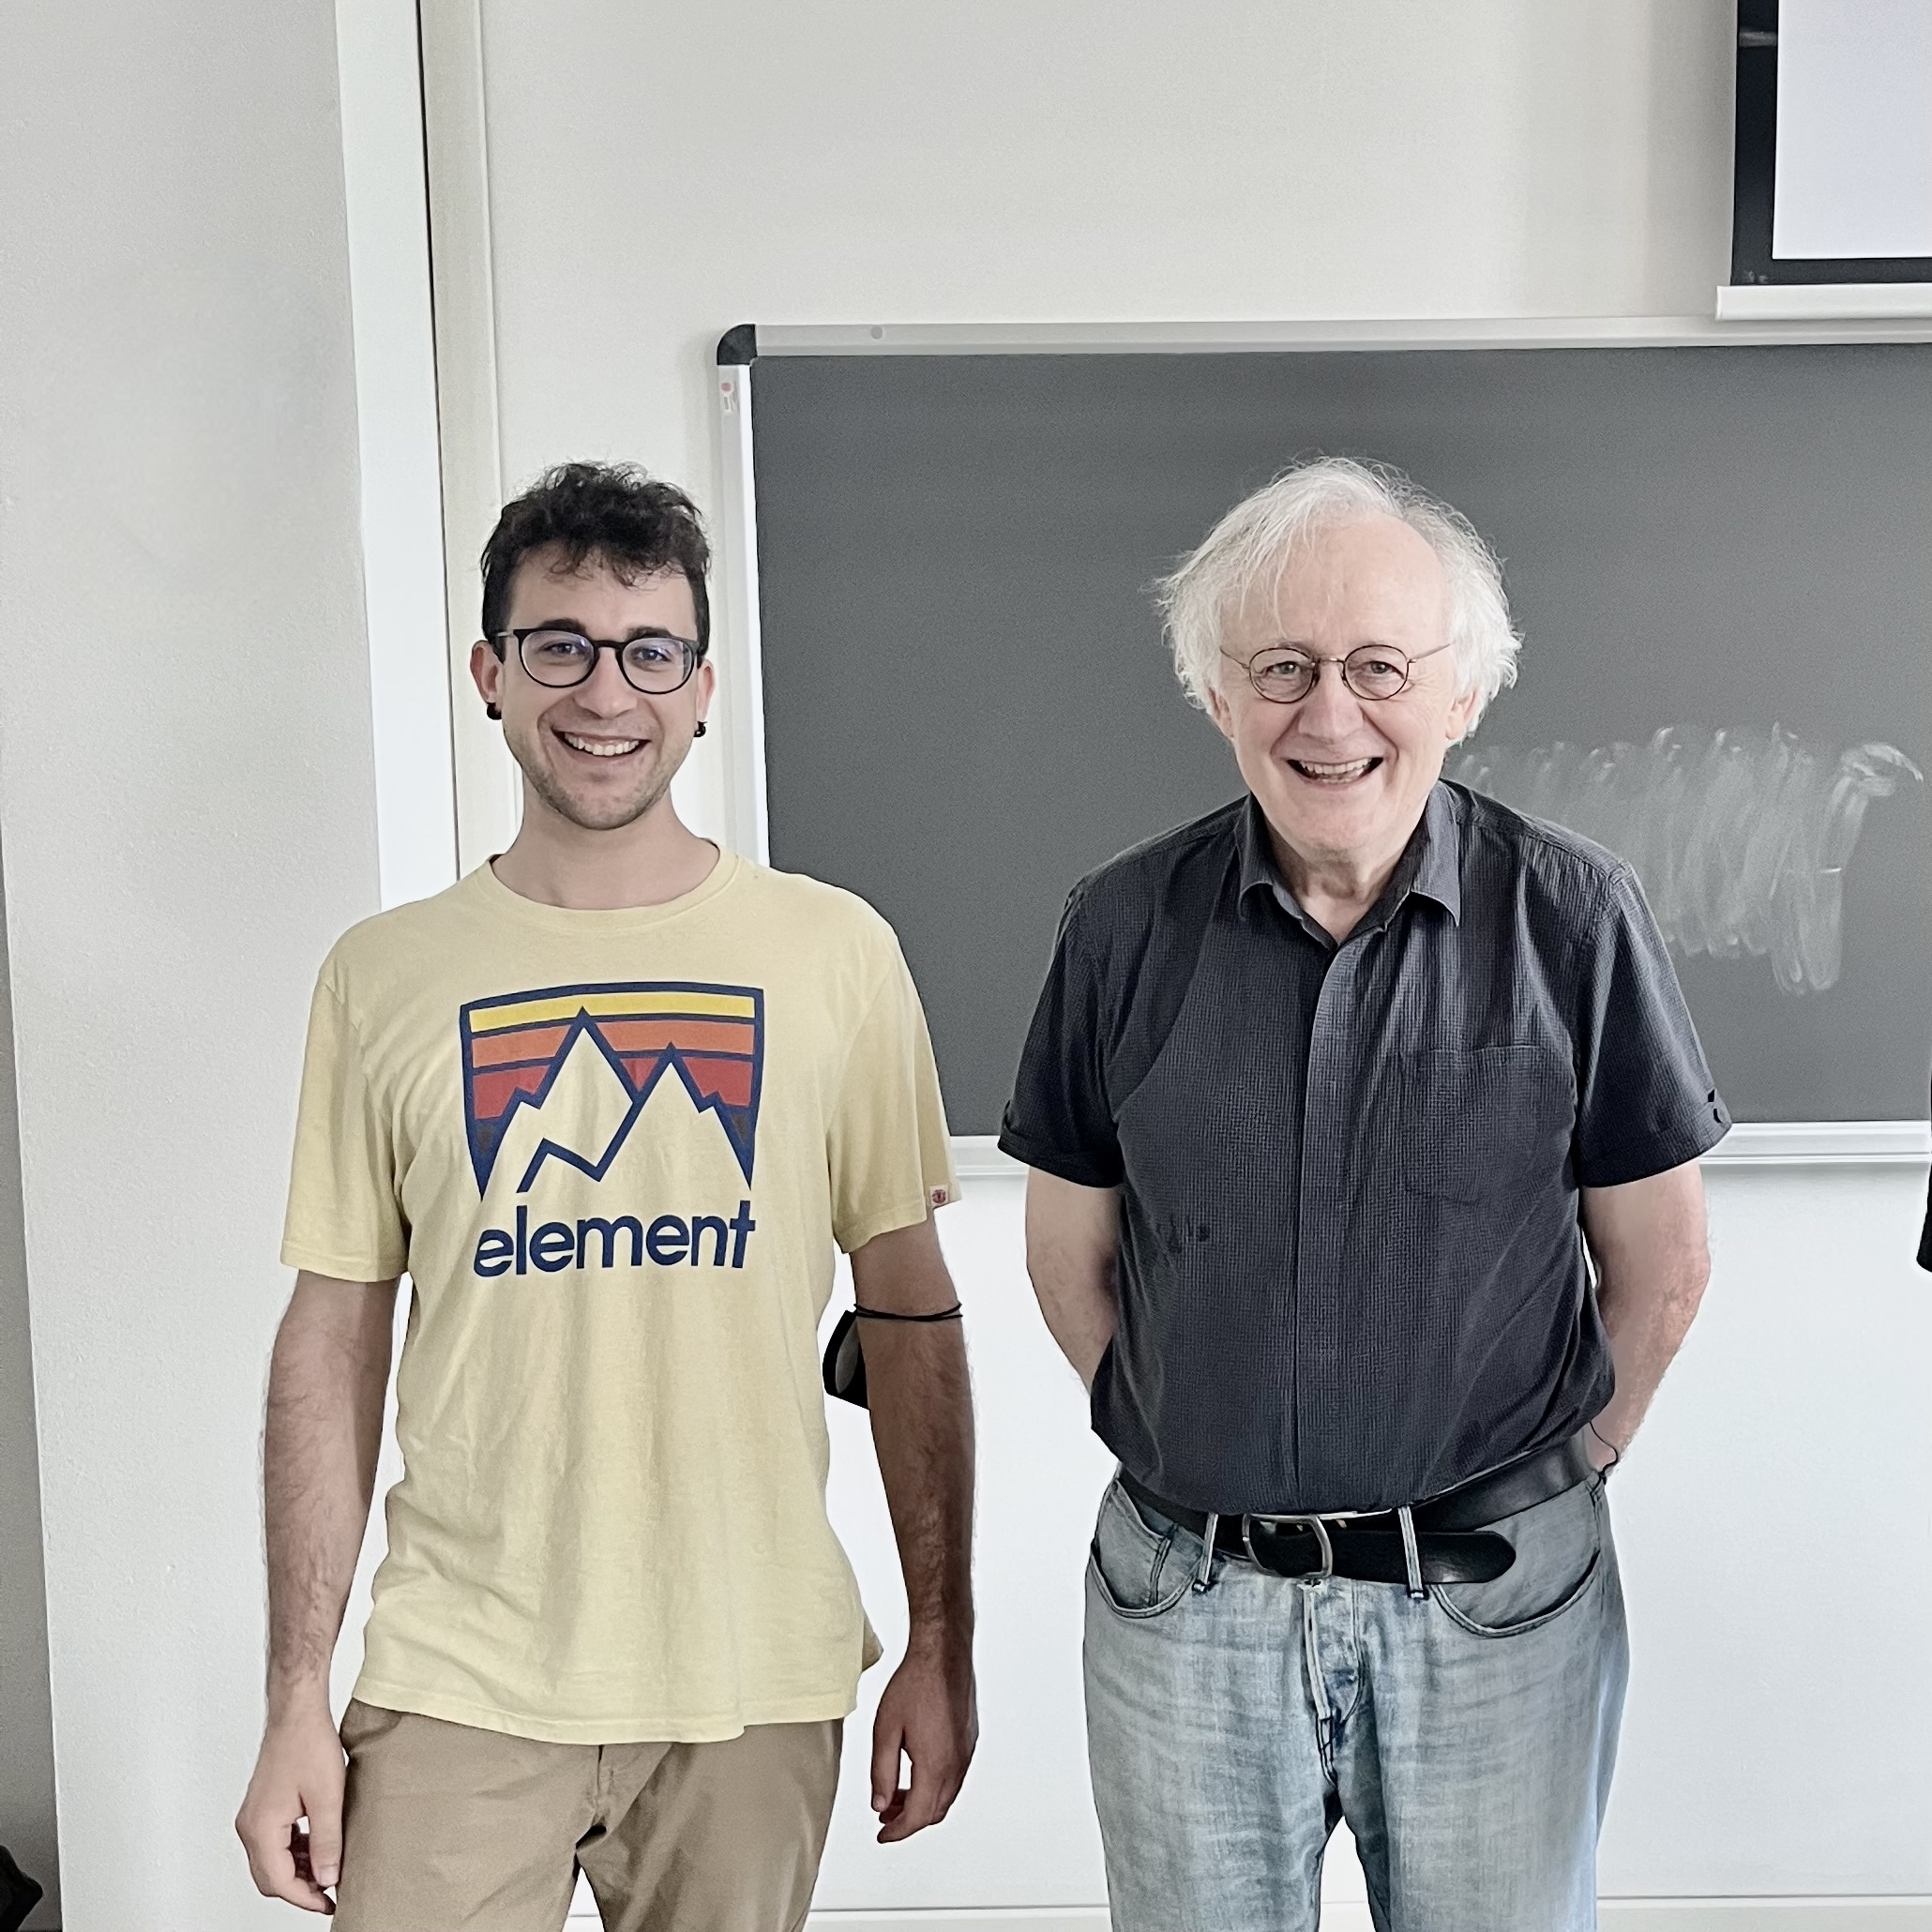
\includegraphics[width=\linewidth + \ClipSep]{figures/denis-patrick}};
    \draw [white, rounded corners=\ClipSep, line width=\ClipSep]
        (current bounding box.north west) --
        (current bounding box.north east) --
        (current bounding box.south east) --
        (current bounding box.south west) -- cycle
        ;
    \end{tikzpicture}
    \vspace*{-\ClipSep}
  % 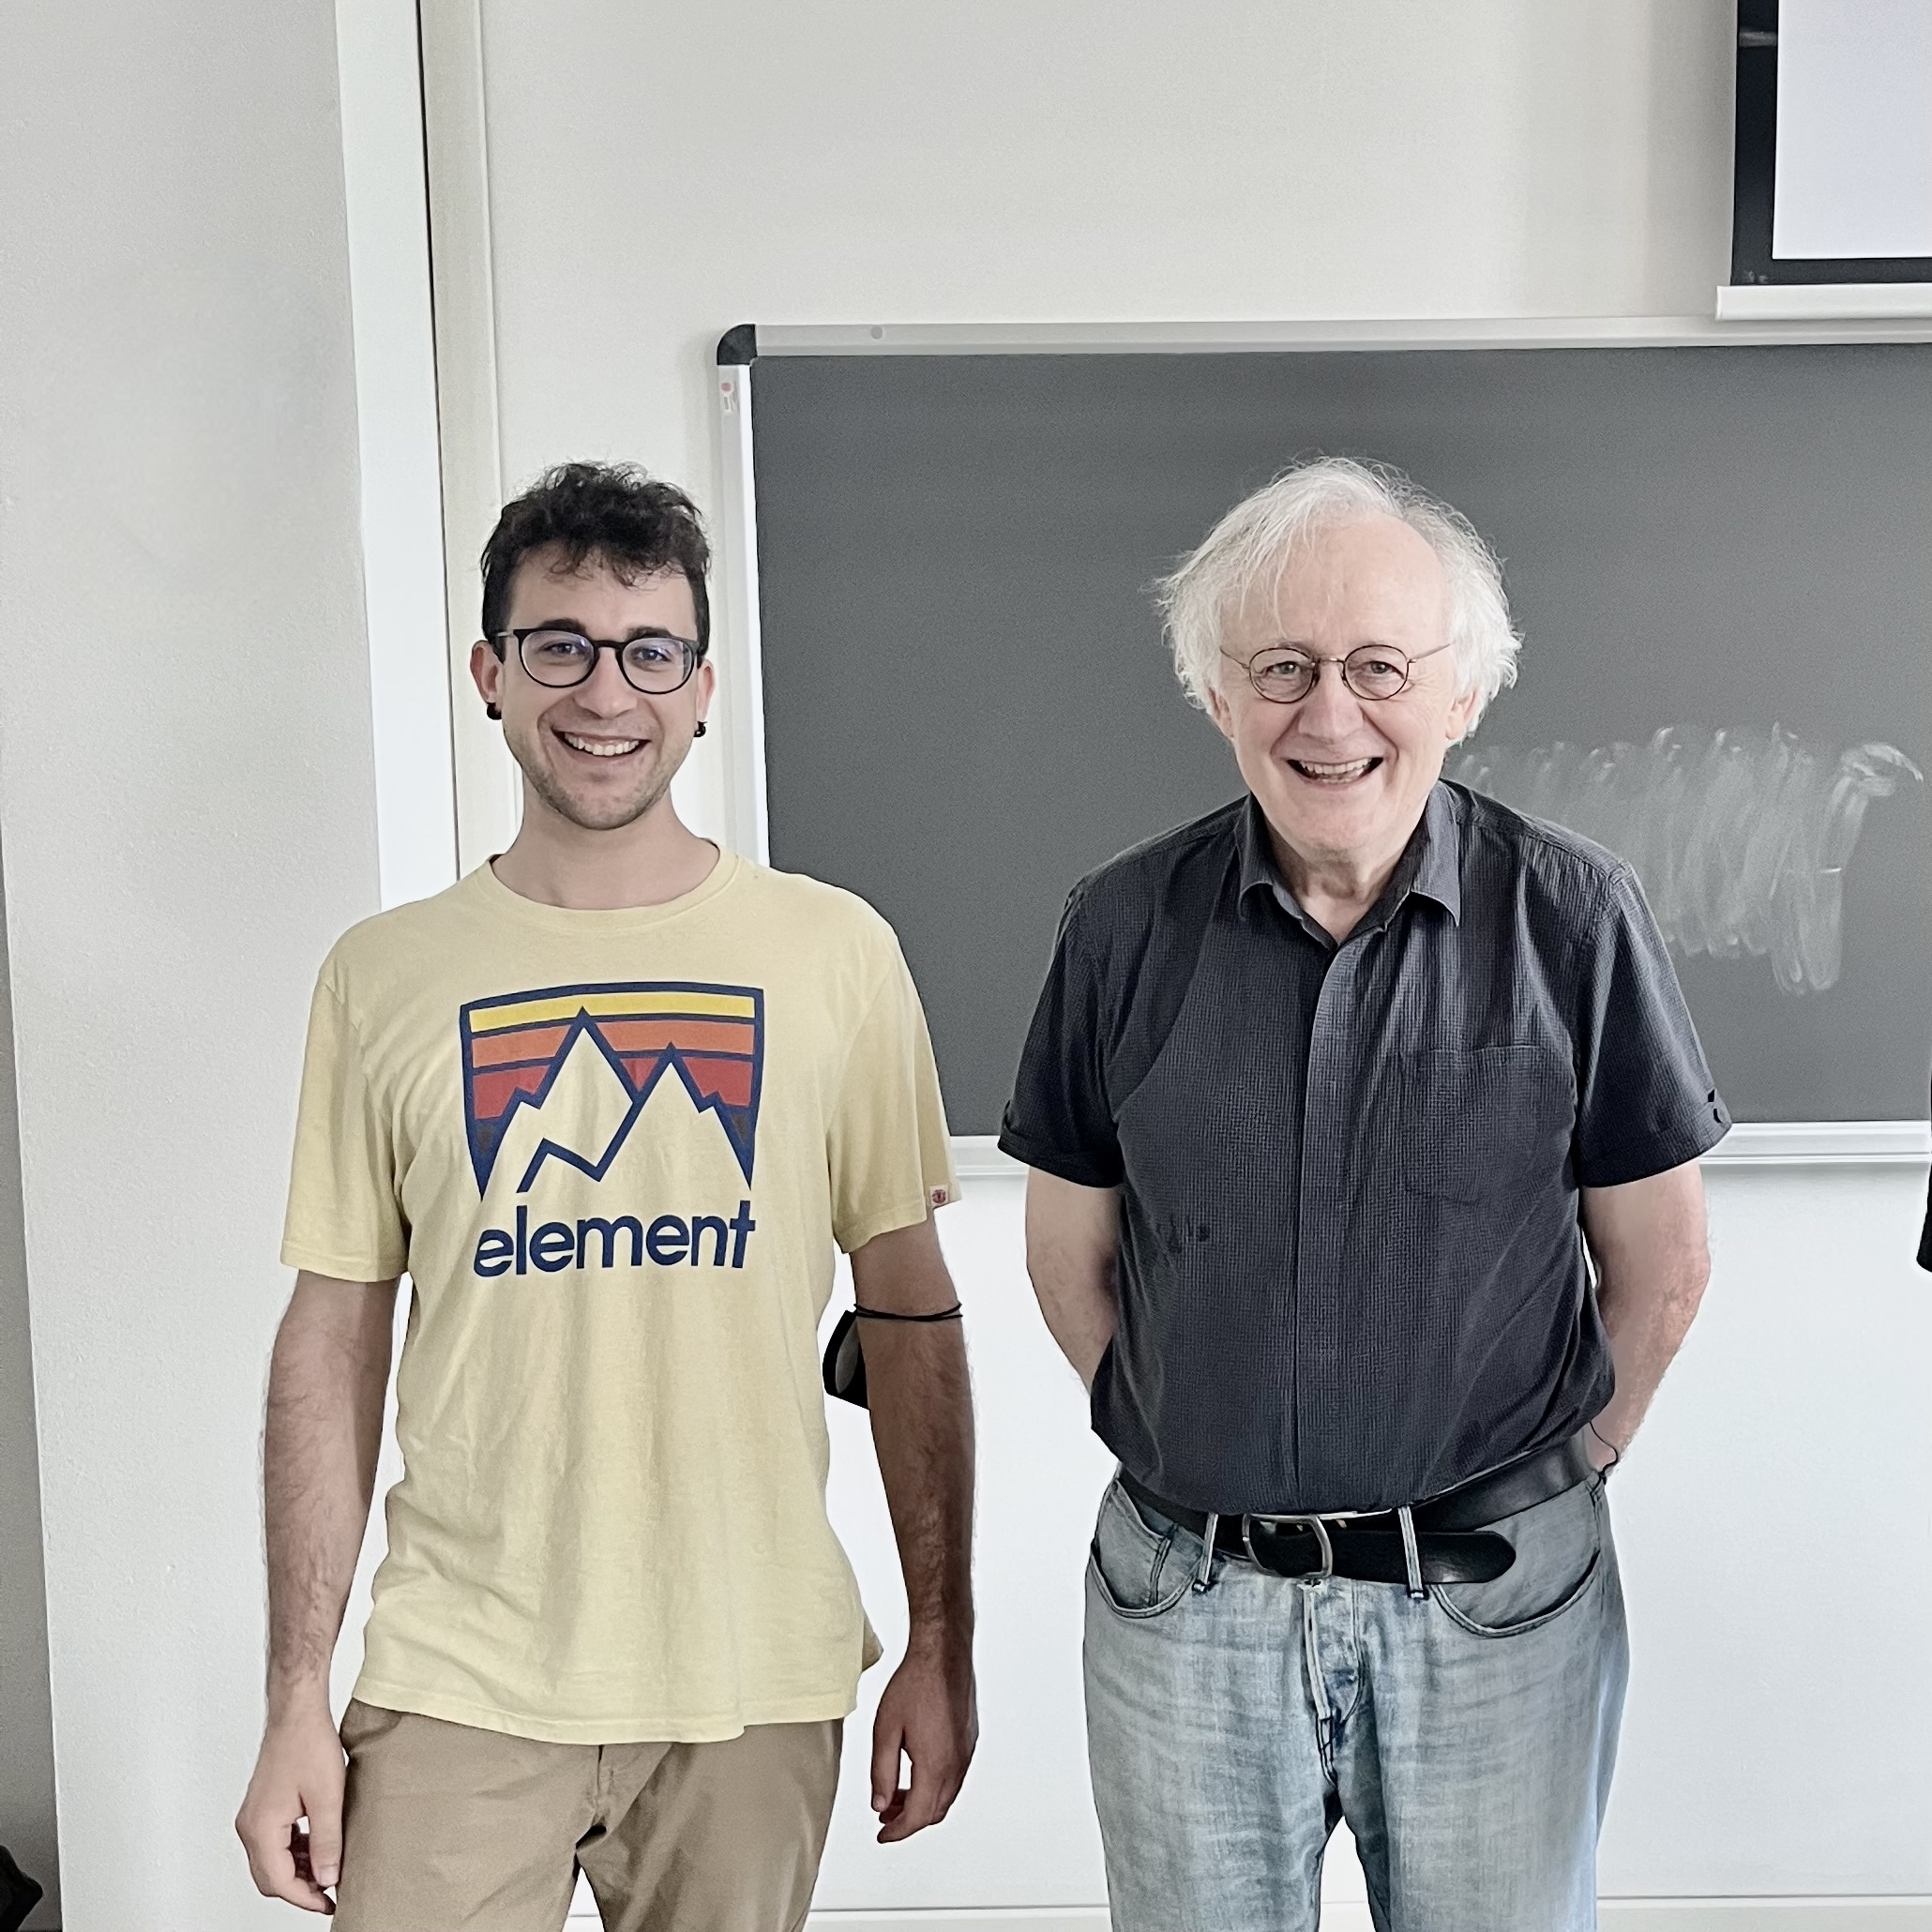
\includegraphics[width=\textwidth]{figures/denis-patrick}
  \caption{Me (left) with Patrick Cousot (right) co-founder of abstract interpretation \cite{\absintkey}.}
  \labfig{denis-patrick}
\end{marginfigure}

\emph{Why the narrow main text column?} It is all about the wide margin: an expansive playground for notes, code snippets, figures, tables, citations, and all those additional details that enhance the narrative, as \reffig{denis-patrick} shows.
This layout lets the main narrative to take the spotlight while all the extra bits are placed in the margin, where they can be easily accessed without disrupting the flow of the text. It is like having a personal assistant handing you the information right when you need it.

With over 200 references in this manuscript, the use of side references becomes a lifesaver.
The hassle of digging back and forth through the bibliography to remember which citation matches \sidecite{\customcitkey} is a thing you will not endure in this thesis.
Speaking of citations, as every computer scientist knows, ``42'' is the answer of Life, the Universe and Everything, according to Douglas Adams' \emph{The Hitchhiker's Guide to the Galaxy}.\sidenote{\rurl{en.wikipedia.org/wiki/Phrases_from_The_Hitchhiker\%27s_Guide_to_the_Galaxy\#The_Answer_to_the_Ultimate_Question_of_Life,_the_Universe,_and_Everything_is_42}}
Right on point, the 42nd citation (in citation order) is where this thesis began. Written by my supervisor Caterina Urban in 2018, \cite{\customcitkey} is the foundational work for the property of input data usage, unifying existing literature on information flow analyses within the formal framework of abstract interpretation\cite{\absintkey}. In essence, \cite{\customcitkey} inspired my academic journey and the last four years of my life.

Note how multiple citations of the same work are automatically merged in the margin, for example, \cite{\customcitkey} in the paragraph above or \cite{\absintkey} within \reffig{denis-patrick}.
Additionally, the template allows for short restatements of definitions and theorems, linked to their original appearances.
Readers will not flip through the pages up and down this manuscript--once a concept is introduced, it conveniently pops up in the margin whenever relevant again.
Recalling what was \refdef*{complete-lattice} has never been easier, just a look in the margin.
For the \textsc{pdf} version of this thesis, you can also click on the title of the margin definition to jump to its original appearance in the text.
This keeps the discussion clear and accessible, which is especially valuable in a complex and detailed work like a PhD thesis. In short:
\begin{center}\itshape
this wide-margin template makes navigating through these pages a bit easier, \\
and hopefully, a bit more enjoyable too.
\end{center}


\mainmatter % Denotes the start of the main document content, resets page numbering and uses arabic numbers

\chapter{Introduction}
\labch{introduction}

Recent advances and evolution in software development have made software more and more complex.
The reliability of software systems is based on their correctness.
Any failure or vulnerability in software poses a significant risk, potentially threatening human safety and causing financial losses.
Nowadays, with more complex systems, the likelihood of software containing bugs increases.
The effort and cost to fix bugs grow with late detection, \reftab{effort-to-fix} illustrates the relative costs of fixing bugs at different development stages.
Nowadays, software rules safety-critical systems such as nuclear power plants, car engines, airplane control systems, and medical devices.
For system where safety is critical, addressing bugs before deployment is mandatory.


Nowadays, machine learning software has an ever-increasing societal impact by assisting or even automating decision-making in fields such as social welfare, criminal justice, and even health care.
At the same time, a number of recent cases have shown that such software may reproduce, or even reinforce, bias directly or indirectly present in the training data \cite{BuolamwiniGebru2018,KayMatuszek2015,COMPAS,ObermeyerPowers2019}.
In April 2021, the European Commission proposed a first legal framework on machine learning software -- the Artificial Intelligence Act~\cite{ArtIntAct}
--- which imposes strict requirements to minimize the risk of discriminatory outcomes.

Moreover, recent advancements in artificial intelligence have led to the rise of large language models (LLMs) capable of generating software from natural language specifications. Agents like OpenAI's ChatGPT and Google's Gemini are gaining widespread use. Specifically designed for coding, GitHub Copilot assists programmers within IDEs and has over a million subscribers. Despite their benefits, AI-generated code can introduce as many bugs as human-written code, making it crucial to use techniques that detect software errors or certify intended behaviors.

\section{Software Quality}

Software quality is a measure of how well software meets its requirements.
The most common method to ensure software quality is \emph{testing}.
The correct behavior of software is tested empirically for finite number of inputs against a set of assertions that specify the functional requirements of the code.
However, testing has inherent limitations.
Testing can only verify a program against the functional requirements, which may be poorly defined and ambiguous, leading to inadequate testing.
Exhaustive testing of systems is impractical, and constraints on time and budget can further impact the process.
But mostly, testing is not sufficient to guarantee the absence of bugs in software\sidenote{``program testing can be quite effective for showing the presence of bugs, but is hopelessly inadequate for showing their absence.'' -- Edsger W. Dijkstra \cite{Dijkstra1976}}.
While in some cases it is acceptable to deploy software with bugs (and rely on patches to fix them, \reftab{effort-to-fix}), in the case of safety-critical systems, it is necessary to ensure that the software is free of bugs before deployment to avoid catastrophic consequences.

In contrast, \emph{formal methods} provide rigorous mathematical guarantees about the correctness of software.
Thanks to their mathematical foundation, an approach based on formal methods guarantees 100\% accuracy in the verification of software properties.
The idea of formally verifying software is not new, and it has been around since the late 1960s with program proofs and invariants from \sidetextcite{Floyd1967} and \sidetextcite{Hoare1969}.
Even before, formal methods may be traced back to the work of \sidetextcite{Church1936} and \sidetextcite{Turing1936} on the foundations of computation.
According to software engineering practices, formal methods can be introduced early in the development lifecycle, enabling the verification of software properties at the design stage.
%
\begin{center}\em
  Why should formal methods replace other well-known, widely accepted, and user-friendly techniques such as testing?
\end{center}
To answer this question, we provide examples where testing failed.


Ariane 5 rocket failure\sidenote{\url{https://esamultimedia.esa.int/docs/esa-x-1819eng.pdf}} in 1996 caused by an integer overflow bug resulting in a loss of \$370 million.
Airfrance Flight 447 crashed in June 2009, killing hundreds of passengers, due to a probe sensor that were not able to accurately measure the airplane speed, which in turns disengaged the autopilot. The probe fault was not detected during testing as the test engineers assumed that such an event was impossible to happen.
Similarly, the Therac-25 radiation therapy\sidecite{Leveson1993} machine where at least six patients received massive overdoses of radiation due to race conditions.
The Toyota unintended acceleration\sidenote{\url{https://www.embeddedrelated.com/showarticle/1574.php}} case where a stack overflow resulted in the death of 89 people and a lawsuit of \$1.2 billion.
The roundoff error in the Patriot missile system\sidenote{\url{https://www.ima.umn.edu/~arnold/disasters/patriot.html}} that caused the death of 28 people during the Gulf War.
All these cases could have been avoided with formal methods.

Unlike testing, formal methods enable exhaustive investigation and detection of bugs that testing may miss. The actual system requirements are translated into formal specifications, which are mathematically verified to ensure the system's behavior aligns with real-world scenarios.
However, Rice's undecidability theorem \sidecite{Rice1993} states that all non-trivial properties\sidenote{
  A property is non-trivial if it is not true for all programs or false for all programs.
} are undecidable, which means that there is no terminating algorithm that can decide whether a program satisfies a non-trivial property.
Therefore, as a consequence of Rice's theorem, formal methods either sacrifice \emph{completeness}, \emph{soundness}, or \emph{automation}.
Current formal methods can be classified into three categories\sidecite{Cousot2010}: \emph{theorem provers}, \emph{model checking}, and \emph{static analysis}.



\begin{marginfigure}
  \centering
  \begin{tikzpicture}[scale=0.8]
    % Draw the triangle
    \draw[thick] (0,0) -- (4,0) -- (2,4) -- cycle;

    % Place the vertices with blue squared borders
    \node[draw, fill=white, text width=2.4cm, align=center, draw=white] at (0,0) {\footnotesize \textsc{Automation}};
    \node[draw, fill=white, text width=2cm, align=center, draw=white] at (4,0) {\footnotesize \textsc{Soundness}};
    \node[draw, fill=white, text width=2.6cm, align=center, draw=white] at (2,4) {\footnotesize \textsc{Completeness}};

    % Place the edges' labels inside the edges
    \node[fill=white, text width=1.5cm, align=center] at (2,0) {\footnotesize Static Analysis};
    \node[fill=white, text width=1.5cm, align=center, rotate=60] at (1,2) {\footnotesize Model Checking};
    \node[fill=white, text width=1.8cm, align=center, rotate=-60] at (3,2) {\footnotesize Theorem Provers};
\end{tikzpicture}
  \caption{Trade-offs in formal methods.}
  \labfig{formal-methods-trade-offs}
\end{marginfigure}

Theorem provers produce proofs of correctness employing interactive tools, also called proof assistants, such as Coq, Isabelle, and HOL Light, or automatic ones like \dots
Ultimately, user interaction is required to guide the proof search.
Even in automatic theorem provers, where automation is key design, to verify any general property, user interaction is required at some point.
Theorem provers are complete and sound, but they are not fully automated.

Formal methods based on model checking explore completely and automatically the state space of a program's model to verify whether undesirable states are reachable.
\sidetextcite{Clarke2004} apply model checking to prove the correctness of ANSI-C programs.
However, model checking-based methods are limited by the state explosion problem: since the number of feasible execution paths grows exponentially with the size of the model, this category of formal methods trade soundness for completeness and automation.

Static analysis is a category of formal methods that analyze without user interaction the program source code to some level of abstraction.
This abstraction is sound but incomplete, meaning that the analysis may report \emph{false alarms}, \ie, warnings that a correct program may be incorrect. However, whenever the static analysis certifies the absence of a bug, the program is indeed bug-free.
The most common static analysis techniques are based on \emph{abstract interpretation}.

Abstract Interpretation \sidecite{Cousot1977} is a general theory for approximating the program semantics, developed by Patrick and Radhia Cousot in the late 1970s.
Their framework is based on the observation that to reason about program properties, not all the computational details are necessary.
Instead, the program's semantics can be approximated by a simpler, more abstract model that facilitate the automatic reasoning.

Over the past decade, abstract interpretation-based static analyses have been successfully applied to the development cycle of real-word software.
The \emph{Astrée} static analyzer \sidecite{Cousot2005} is routinely used to ensure the absence of runtime errors in embedded synchronous C programs for the Airbus A340 and A380.

We provide a formal introduction to abstract interpretation in \refch{abstract-interpretation},
and we recall the main results used in this thesis, which are later illustrated
on a small idealized programming language at the end of the same chapter.


\section{Input Data Usage}

In software systems, programming errors do not always result in crashes or runtime errors.
It may be the case that the faulty program produces a plausible yet erroneous outcome or unsafe behavior.
Such bugs are hard to spot since they provide no clear indication that something went wrong.
A potential source of such errors is the misuse of input data, \ie, when an input variable has an unexpected impact on the program computation compared to the developers' expectations.

A notable example is the Reinhart and Rogoff article ``Growth in a Time of Debt'' \sidecite{Reinhart2010}, which claimed that economic growth is negatively correlated with public debt.
This article was heavily cited to justify austerity measures around the world in the following years.
However, in 2013, \sidetextcite{Herndon2013} discovered that the authors had made a mistake in their Excel spreadsheet, which led to the erroneous conclusion.
Notably, one of the several programming and methodological errors discovered is the incorrect usage of the input value relative to Norway's economic growth in 1964, with an excessive weight in the computation of the average growth rate.

Particularly in the context of data science applications, where software involves long pipeline of layers that filter, merge, and manipulate data, the likelihood of programming errors that cause some input variables to be more, or less, in fluent than what was expected is high.
Hence, it is important to employ techniques that enhance the confidence in the usage of input variables for data-driven applications.

\refch{input-data-usage} introduces the input data usage property, which is a formal property that captures the \emph{qualitative} usage of input data in a program.

\section{Quantitative Properties}

Commonly, in the context of properties of programs, a program either satisfies a property or not.
Such qualitative restriction is not sufficient to capture the complexity of real-world requirements.
Consider for instance one of the most fundamental security issues: protecting the confidentiality of sensitive information.
In secure information flow analysis the question is whether a program could leak information about its secrets.
A classic approach, based on any of the formal methods explored above, would try to enforce \emph{noninterference}, certifying that a program reveals no information about its secrets.
Unfortunately, noninterference is too strict for many practical applications.
In the case of a digital election protocol, individual votes should be anonymous, but of course the final result needs to be revealed. A password checker should not reveal the password, but it should reveal whether the password is correct.
These cases represent deliberate violations of noninterference that are necessary for the program to fulfill its purpose.

To address this limitation, one approach is to consider quantitative properties.
The key idea is to accept that a program may violate a property, and compare such violation against a threshold.
Programs are classified as \emph{safe} or \emph{unsafe} based on the degree of violation, thus inducing a classification among programs based on how much safety they provide.


In the Reinhart and Rogoff case, the value of Norway's economic growth was indeed used in the average computation, but its impact was much higher than it should have been.
The error was not whether the value was used or not, but rather how much it was used.
In this case, a quantitative analysis would have revealed that the impact of Norway's economic growth was too high, and the authors could have corrected the wrong conclusion.

\refch{quantitative-input-data-usage} introduces the formal framework, based on abstract interpretation, to reason about quantitative properties of programs of input data usage.


\section{Contributions and Outline}

In this thesis, we study techniques based on formal reasoning to detect misuse of input data.
We propose semantics-based static analysis techniques to soundly quantify the impact of input variables on the program computation.
\refch{abstract-interpretation} provides the mathematical background used in the rest of the thesis and introduces the formal framework of abstract interpretation.
The rest of this section outlines the organization of the thesis.

\subsection{Input Data Usage}

In \refch{input-data-usage}, we focus on the definition of the input data usage property. Specifically, we introduce its definition as proposed by \sidetextcite{Urban2018}.
Then, we extend the property to capture abstractions of output values as done in the generalization of non-interference property \sidecite{Giacobazzi2018}.
We provide the hierarchy of semantics that precisely captures the input data usage property abstracting unnecessary details.
Finally, from \textcite{Urban2018} we report an abstract semantics that captures syntactic dependencies between variables, which is used to soundly approximate the input data usage property.

\subsection{Quantitative Input Data Usage}

In \refch{quantitative-input-data-usage}, we present a novel quantitative input usage framework to discriminate between input variables with different impact on the outcome of a program.
This framework can be used to identify variables that have a disproportionate impact.
Such knowledge could either certify intended behavior or reveal potential flaws, by matching the developers' intuition on the expected impact of their input with the actual result of the quantitative study.
We characterize the impact of an input variable with a notion of dependency between variables and the outcome of a program.
In general, determining how an input variable influences a program outcome depends on several factors, such as the structure of the program, the environment, the expertise of the developer, and the intuition of the researcher.
Consequently, there is no single impact definition that fits all requirements. For this reason, our framework is parametric in the impact definition of choice.

Building on this framework, we introduce a backward static analysis based on abstract interpretation parametric in the definition of impact, which automatically infers a sound over-approximation of the impact of input variables when analyzing programs. We design our static analysis to soundly approximates our property, by returning an upper bound on the impact quantity.
The inputs of our static analysis consist of a set of cumulative ranges representing program outputs, called output buckets.
Then, the analysis backward computes the input states leading to these buckets and applies a computable implementation of the impact on the result of the backward reachability analysis.
This approach allows end-users to choose the impact that best fits their needs, ensuring a more targeted and customizable analysis.

This chapter is based on work published at NASA Formal Methods Symposium
(NFM) 2024 \sidecite{Mazzucato2024nfm}.


\subsection{Quantitative Verification for Neural Networks}

In \refch{quantitative-fairness}, we extend the quantitative input data usage property to the domain of neural networks.
We propose two impact notions for neural networks. The first one addressing the ragged input space of neural networks, and the second one measuring the amount of fairness of input features.
First, we show how a na\"ive approach measures the impact of input features in neural networks, and then we refine the backward analysis to exploit parallel computations and achieve better performance.

Our approach employs a combination of forward and backward analyses.
The forward pass aims to reduce the combinatorial explosion the backward analysis faces when analyzing neural-network models.
The static analysis revolves around the concept of \emph{independent input partitions}, partitioning the input space into subregions that are easier to analyze for the backward analysis and do not interfere with each other, allowing parallel computations.
Moreover, the forward analysis can be configured in terms of scalability and precision to adapt to the user's needs. By the choice of abstract domain and budget of resources, the analysis trades off precision for execution time.
The resource budget can be auto-tuned to find the best analysis configuration according to a given search heuristic.

This chapter is based on work published at the 28th Static Analysis Symposium (SAS) 2021 \sidecite{Mazzucato2021}.

\subsection{Quantitative Static Timing Analysis}

In \refch{quantitative-static-timing-analysis}, we consider the amount of program iterations during the execution of a program as the program outcome.
Thus, we capture the impact of input variables on the \emph{global} number of iterations of a program.
Such variation is interesting as programming errors related to the misuse of input data affecting the number of iterations may degrade performance or introduce security vulnerabilities without even showing any functional error.
For instance, in the context of security, an unexpected impact of input variables on the program's runtime could reveal sensitive information \sidecite{Wong2005}, leading to potential security threats.
Even in cryptography, where programs are mathematically robust, vulnerabilities to timing attacks persist, depending on the implementation choices and design.
\sidetextcite{Kocher1996} demonstrated that widely used public key cryptographic algorithms, like RSA, are vulnerable to timing attacks, and may leak information about the secret key.
The value of such attacks lies in their simplicity;
attackers do not need to possess detailed knowledge of the program implementation or engage in computationally expensive operations.
Merely the information of which primitives are used in the program is enough.
For example, knowledge that the exponentiation operation, commonly found on cryptographic programs, is performed using the square-and-multiply algorithm can enable an attacker to exploit the program's runtime to infer the secret key \sidecite{Wong2005}.
Indeed, \sidetextcite{Dhem2000} mounted such attack against CASCADE smart cards, observing timing differences during the square operations of the square-and-multiply algorithm.
Furthermore, knowing the timing behavior of a program could certify intended behavior or reveal latent flaws by matching developers' expectations with the actual program behavior.
For performance optimization, identifying input variables that most significantly affect loop iterations can help developers focus on critical code segments \sidecite{Omar2017}.
As a consequence, achieving a comprehensive understanding of the impact of input variables on the program runtime is paramount.
In this study we focus on quantifying the impact of input variables on the number of loop iterations in a program, as an indicator of the program's runtime behavior.


In this chapter, we leverage an underlying global loop bound analysis to derive an over-approximation of the global loop bound and encode the quantification of each input variable's impact as a linear programming problem.
Our approach blends syntactic and semantic information:
to improve accuracy, the global loop bound analysis generates invariants as a set of linear constraints;
to improve scalability, we combine the global loop bound analysis with a syntactic dependency analysis \sidecite{Urban2018}, reducing the number of variables to analyze.

This chapter is based on work published at the 31st Static Analysis Symposium (SAS) 2024 \sidecite{Mazzucato2024sas}.

\subsection{Contributions}

The main contributions of this thesis are as follows:
\begin{itemize}
  \item In \refch{input-data-usage} we extend the original definition of the input data usage property to capture abstractions of output values.
  Such extension blends generalized non-interference with input data usage, providing a definition that works also for non-deterministic programs.
  \item In \refch{quantitative-input-data-usage}
\end{itemize}



\chapter{Abstract Interpretation}
\labch{abstract-interpretation}

\section{Order Theory}
\labsec{order-theory}

\subsection{Sets}
\labsec{sets}

\subsection{Relations}
\labsec{relations}

\subsection{Ordered Sets}
\labsec{ordered-sets}

\subsection{Lattices}
\labsec{lattices}

\subsection{Functions}
\labsec{functions}

\subsection{Fixpoints}
\labsec{fixpoints}

\section{Notations of Abstract Interpretation}
\labsec{notations-of-abstract-interpretation}

\subsection{Transition System}
\labsec{transition-system}

\begin{definition}[State]\labdef{state}
  \begin{align*}
    \state \IN \variables \to \values
  \end{align*}
\end{definition}

\subsection{Maximal Trace Semantics}
\labsec{maximal-trace-semantics}

\begin{definition}[Maximal Trace Semantics]\labdef{maximal-trace-semantics}
  \begin{align*}
    \tracesemanticsnoparam &\DefeQ \lfp \tracetransformer \\
    \tracetransformer(\defsetoftraces) &\DefeQ \finalstates \setjoin (\mergesequences{\transitionrelation}{\defsetoftraces})
  \end{align*}
\end{definition}

\subsection{Collecting Semantics}
\labsec{collecting-semantics}

\begin{definition}[Collecting Semantics]\labdef{collecting-semantics}
  \begin{align*}
    \collectingsemanticsnoparam &\DefeQ \{\spacearound{\tracesemanticsnoparam}\}
  \end{align*}

\end{definition}

\subsection{Verification Framework}
\labsec{verification-framework}

\begin{definition}[Validation]\labdef{validation}
  \begin{align*}
    \defprogram \satisfies \defproperty \IfF \collectingsemantics \subseteq \defproperty
  \end{align*}
\end{definition}

\subsection{Fixpoint Induction}
\labsec{fixpoint-induction}

\subsection{Hierarchy of Semantics}
\labsec{hierarchy-of-semantics}

\subsection{Galois Connection}
\labsec{galois-connection}

\subsection{Reachable State Semantics}
\labsec{reachable-state-semantics}

\subsection{Fixpoint Transfer}
\labsec{fixpoint-transfer}

\subsection{Fixpoint Approximation}
\labsec{fixpoint-approximation}

\subsection{Widening}
\labsec{widening}

\subsection{Narrowing}
\labsec{narrowing}


\section{A Small Imperative Language}
\labsec{a-small-imperative-language}

\subsection{Syntax}
\labsec{syntax}

\subsection{Maximal Trace Semantics}
\labsec{maximal-trace-semantics}

\subsection{Numerical Abstract Domain}
\labsec{numerical-abstract-domain}

\subsubsection*{Sign}

\subsubsection*{Boxes}

\subsubsection*{Conjunctions of Linear Constraints}

\subsection{Reduced Product}
\labsec{reduced-product}

\subsection{Forward Reachability State Semantics}
\labsec{forward-reachability-state-semantics}

\subsection{Backward Reachability State Semantics}
\labsec{backward-reachability-state-semantics}

\chapter{Input Data Usage}
\labch{input-data-usage}


In this chapter, we introduce the notion of input data usage as proposed by \textcite{Urban2018}.
In particular, we include output abstractions in the definition of an unused input variable obtaining a more general definition.
Then, we present a \emph{sound and complete} hierarchy of semantics that contain only, and exactly, the information needed to reason about the usage of input variables.
Later in the next chapters, we will define a quantitative measure of usage of input variables, extending the qualitative notion presented in this chapter.

\emph{Dans ce chapitre, nous introduisons la notion d'utilisation des données d'entrée comme proposé par \sidetextcite{Urban2018}. En particulier, nous incluons des abstractions de sortie dans la définition d'une variable d'entrée inutilisée, obtenant ainsi une définition plus générale. Ensuite, nous présentons une hiérarchie \emph{correcte et complète} de sémantiques qui contiennent uniquement et exactement les informations nécessaires pour raisonner sur l'utilisation des variables d'entrée. Plus tard, dans les chapitres suivants, nous définirons une mesure quantitative de l'utilisation des variables d'entrée, en étendant la notion qualitative présentée dans ce chapitre.}

\section{Input Data Usage}
\labsec{input-data-usage}

Originally introduced by \textcite{Urban2018}, the notion of input data usage is a predicate to determine whether the input variable $\definputvariable\in\inputvariables$ is used in the computation of the output. It consists in a predicate
\[
  \unusedwrapper \in \tracetype \to \B
\]
that holds whenever the input variable $\definputvariable\in\inputvariables$ is not used in the program under evaluation.

\begin{definition}[Unused]\labdef{unused-predicate}
  Given a program $\defprogram$, and an input variable of interest $\definputvariable\in\inputvariables$, the variable $\definputvariable$ is \emph{unused} if the following predicate holds:
  \begin{eqnarray*}
    \lefteqn{\unusedwrapper(\tracesemantics) \DefifF} \\
    & &\forall
      \defseq\in\tracesemantics, \defvalue\in\values
    .\spacer
      \retrieveinput{\defseq}(\definputvariable) \neq \defvalue \ImplieS \\
      & &\exists
        \defseq'\in\tracesemantics
      .\spacer
        \retrieveinput{\defseq'} \stateeq{\inputvariableswithouti} \retrieveinput{\defseq}
        \LanD
        \retrieveinput{\defseq'}(\definputvariable) = \defvalue
        \LanD
        \retrieveoutput{\defseq} = \retrieveoutput{\defseq'}
  \end{eqnarray*}
\end{definition}

Intuitively, an input variable $\definputvariable$ is unused if all feasible outcomes $\retrieveoutput{\defseq}$ are feasible from all possible initial values of $\definputvariable$.
That is, for all possible initial values $\defvalue$ that differ from the initial value of $\definputvariable$ in the trace $\defseq$, there exists another trace $\defseq'$ with initial value $\defvalue$ for $\definputvariable$ that leads to the same output $\retrieveoutput\defseq$.

\begin{example}\labexample{school-year}
\begin{marginlisting}[*-9]
  \caption{Program to check if a student passed the school year.}
  \labprog{school-year}
  \vspace{2\lineheight}
\begin{lstlisting}[language=Python,escapechar=|]
is_passed(eng, math, science,
    bonus):
  passing = True;
  if not eng:
    eng = False;|\labline{err1}|
  if not math:
    passing = bonus;
  if not math:|\labline{err2}|
    passing = bonus;
\end{lstlisting}
\end{marginlisting}
Let us consider the program of example presented in \textcite{Urban2018}, \cf{} \refprog{school-year} on the side.
Based on the boolean-valued input variables \texttt{eng}, \texttt{math}, \texttt{science}, and \texttt{bonus}.
The program should determine whether a student has passed the year or not, and store the result in the variable \texttt{passing}. Additionally, the student is allowed a bonus to help with math and science.
However, there are two mistakes in the program: it should be \texttt{passing = False} in the first conditional statement (\cf{} \refline{err1}), and the third condition should be \texttt{not science} instead of \texttt{not math} (\cf{} \refline{err2}).
These two mistakes cause the variables \texttt{eng} and \texttt{science} to be unused in \refprog{school-year}.
Let us consider the input variable \texttt{science}.
The simplified trace semantics, considering only the variables \texttt{science} and \texttt{passing}, is:
\begin{align*}
  \tracesemanticsnoparam\semanticsof{\texttt{is\_passed}_\texttt{science}}
  =
  \left\{
    \begin{array}{l}
      \tuple\true\anyvalue\rightarrow\tuple\true\true, \\
      \tuple\true\anyvalue\rightarrow\tuple\true\false, \\
      \tuple\false\anyvalue\rightarrow\tuple\false\true, \\
      \tuple\false\anyvalue\rightarrow\tuple\false\false
    \end{array}
  \right\}
\end{align*}
where each state $\tuple{\defvalue_1}{\defvalue_2}$ shows the boolean value $\defvalue_1$ of \texttt{science} and $\defvalue_2$ of \texttt{passing}. The symbol $\anyvalue$ denotes any boolean value. We omit the intermediate states for brevity, only showing input-output dependencies.
The input variable \texttt{science} is unused, since each result value for \texttt{passing} is feasible from all possible initial values of \texttt{science}.

Instead, if we consider the variable \texttt{math}, the simplified trace semantics considering only the variables \texttt{math} and \texttt{passing} is:
\begin{align*}
  \tracesemanticsnoparam\semanticsof{\texttt{is\_passed}_\texttt{math}}
  =
  \left\{
    \begin{array}{l}
    \tuple\true\anyvalue\rightarrow\tuple\true\true, \\
    \tuple\false\anyvalue\rightarrow\tuple\false\true, \\
    \tuple\false\anyvalue\rightarrow\tuple\false\false
  \end{array}
  \right\}
\end{align*}
The input variable \texttt{math} is used, since the result value for \texttt{passing} is not feasible from all possible initial values of \texttt{math}.
Indeed, only the initial state $\tuple\false\anyvalue$ yields the result value $\false$ for \texttt{passing} (in the final state $\tuple\false\false$).
\end{example}

\begin{example}
  \begin{marginlisting}
    \caption{Syntactic versus semantic usage of the input variable \texttt{x}.}
    \labprog{syntactic-vs-semantic-usage}
    \vspace{2\lineheight}
  \begin{lstlisting}[language=Python]
x_plus_rand(x):
  return x + rand();
\end{lstlisting}
  \end{marginlisting}
With this second example we highlight the difference between the syntactic and semantic meaning of using a variable. Indeed, a variable could be syntactically used in the program, \ie present in the code, but it could be semantically unused, \ie does not affect the computation of the program; and vice versa.
Consider \refprog{syntactic-vs-semantic-usage} on the side, where the input variable \texttt{x} is a non-negative integer.
The variable \texttt{x} is syntactically used in the program, as it is present in the return statement.
However, the variable \texttt{x} is semantically unused if we consider machine integers wrapped up to $\texttt{max\_int}\in\N$.
This difference can be clearly seen by studying the trace semantics of the program. In case of machine integers the trace semantics is:
\begin{align*}
  \tracesemanticsnoparam\semanticsof{\texttt{x\_plus\_rand}}
  =
  \setdef{
    \langle{x}\rangle\rightarrow\langle{x+r \mod \texttt{max\_int}}\rangle
  }{x, r \in \N}
\end{align*}
where $x\in\N$ denotes the value of the input variable \texttt{x} and $r\in\N$ a random integer from the \texttt{rand()} function.
In this case, any outcome value $x+r \mod \texttt{max\_int}$ is feasible from any initial value of \texttt{x}.
Even if $x$ is bigger than a given outcome $z$, the result is still feasible as we can take a positive $r = \texttt{max\_int} - x + z$ to make the wrapped sum $x + r \mod \texttt{max\_int} = z$.

On the other hand, if we consider unbounded positive integers, the trace semantics is:
\begin{align*}
  \tracesemanticsnoparam\semanticsof{\texttt{x\_plus\_rand}}
  =
  \setdef{
    \langle{x}\rangle\rightarrow\langle{x+r}\rangle
  }{x, r \in \N}
\end{align*}
In such instance, for any outcome value $x+r$, only initial values of \texttt{x} that are equal or smaller than $x+r$ may generate such outcome.
For instance, if the outcome is 42, an initial value of 41 is feasible as it exists a random value $r = 1$ that makes the sum $41 + 1 = 42$. Instead, an initial value of 43 is not feasible as there is no positive random value $r$ that makes the sum $43 + r = 42$.
% \pgfplotstableread[]{
% x y
% 0 81
% 1 15
% 2 5
% 3 97
% 4 39
% 5 36
% 6 34
% 7 24
% 8 102
% 9 22
% 10 96
% 11 105
% 12 81
% 13 24
% 14 89
% 15 69
% 16 20
% 17 20
% 18 29
% 19 46
% 20 49
% 21 85
% 22 99
% 23 26
% 24 95
% 25 50
% 26 117
% 27 110
% 28 117
% 29 98
% 30 83
% 31 59
% 32 89
% 33 108
% 34 69
% 35 35
% 36 133
% 37 57
% 38 127
% 39 93
% 40 83
% 41 76
% 42 61
% 43 70
% 44 141
% 45 88
% 46 59
% 47 58
% 48 96
% 49 61
% 50 95
% 51 95
% 52 129
% 53 86
% 54 59
% 55 148
% 56 114
% 57 125
% 58 73
% 59 107
% 60 70
% 61 131
% 62 99
% 63 143
% 64 143
% 65 111
% 66 139
% 67 91
% 68 158
% 69 77
% 70 75
% 71 155
% 72 101
% 73 171
% 74 111
% 75 85
% 76 105
% 77 89
% 78 126
% 79 114
% 80 138
% 81 162
% 82 128
% 83 103
% 84 131
% 85 130
% 86 112
% 87 172
% 88 122
% 89 178
% 90 177
% 91 173
% 92 101
% 93 170
% 94 175
% 95 116
% 96 164
% 97 190
% 98 129
% 99 119
% }\advdata
% \begin{figure}[H]
% \centering
% \caption{Scatterplot of Advertising versus Sales Data}
% \begin{tikzpicture}
% \begin{axis}[
% axis lines = left,
% xlabel = {Input Variable \texttt{x}},
% ylabel = {Program Outcome}
% ]
% \addplot[
% mark=*,only marks,
% point meta =explicit symbolic,
% nodes near coords,
% ]
% table[x=x,y=y]{\advdata};
% \end{axis}
% \end{tikzpicture}
% \end{figure}
\end{example}

\nrefdef{unused-predicate} is significant as it determines whether a given input variable is used or not, even in the presence of non-deterministic programs%
\sidenote[][*-8]{%
  In \refexample{school-year} the trace semantics where we consider subsets of input variables, \cf{} $\tracesemanticsnoparam\semanticsof{\texttt{is\_passed}_\texttt{science}}$ and $\tracesemanticsnoparam\semanticsof{\texttt{is\_passed}_\texttt{math}}$, are two non-deterministic sets of traces.
  %
  This can be easily seen by considering the two traces:
  \begin{eqnarray*}
    \lefteqn{\tuple\true\true\rightarrow\tuple\true\true} \\
       &\in \tracesemanticsnoparam\semanticsof{\texttt{is\_passed}_\texttt{science}} \\
    \lefteqn{\tuple\true\true\rightarrow\tuple\true\false} \\
       &\in \tracesemanticsnoparam\semanticsof{\texttt{is\_passed}_\texttt{science}}
  \end{eqnarray*}
  where both start from the same initial state $\tuple\true\true$ and have different outcomes.}.
Furthermore, the next example shows that the unused predicate is termination aware.
Indeed, termination is a possible outcome of a program, and thus a variable should be unused if it does not affect the termination as well as the outcome of the program.

\begin{example}\labexample{non-termination}
  \begin{marginlisting}
    \caption{Program that does not terminate for positive values of \texttt{x}.}
    \labprog{non-termination}
    \vspace{2\lineheight}
  \begin{lstlisting}
non_termination(x):
  while x > 0:
    x = x + 1;
\end{lstlisting}
  \end{marginlisting}
  Consider the \refprog{non-termination} defined on the side. The program does not terminate for positive values of \texttt{x}. Instead, it terminates without modifying \texttt{x} on the value of $0$ or negative. The trace semantics is the following:
  \begin{align*}
    \tracesemanticsnoparam\semanticsof{\texttt{non\_termination}}
    =
    \{
      \langle{<}\rangle\rightarrow\langle{<}\rangle,
      \langle{0}\rangle\rightarrow\langle{0}\rangle,
      \langle{>}\rangle\rightarrow\dots
    \}
  \end{align*}
  where the symbol $<$ denotes a negative value and $>$ a positive one. When the program is provided a positive value for \texttt{x}, it does not terminate and the respective traces are all of infinite length.

  In this example we conclude that the variable \texttt{x} is used since the non-termination is feasible only from positive values of \texttt{x}.
  In fact, by excluding non-termination as a possible outcome, the variable \texttt{x} would be, instead, unused.
\end{example}

\section{Abstract Input Data Usage}
\labsec{abstract-input-data-usage}

Inspired by the definition of abstract non-interference (ANI) \sidecite{Giacobazzi2018,Mastroeni2023}, we introduce a generalized version of the unused predicate.
That is, a weaker version of the unused predicate that abstracts the output states, allowing for a more general definition of the unused property.
Later, we will define the quantitative measure of input data usage, and use the abstraction of output states to determine numerical values from output states.

\marginnote{
\begin{definition}[Abstract Non-Interference]\labdef{ani-predicate}
  The abstract non-interference predicate $\aniwrapper$ holds if, for any two traces $\defseq$ and $\defseq'$:
  \begin{gather*}
      \aniselect(\retrieveinput{\defseq}) = \aniselect(\retrieveinput{\defseq'})
      \ImplieS
       \aniobserver(\retrieveoutput{\defseq}) = \aniobserver(\retrieveoutput{\defseq'})
  \end{gather*}
\end{definition}
We assume that the objective of the input abstraction $\aniselect$ is to monitor the interference of the input variable $\definputvariable$.}

In the following, we define the abstraction of output states, called output observer, as a map from states to an abstract domain.

\begin{definition}[Output Observer]\labdef{output-observer}
  Given a program $\defprogram$, an \emph{output observer} $\aniobserver\in \state \to \state$ is an upper closure operator that abstracts the value of output states.
\end{definition}


Similar to the abstraction of non-interference property into abstract non-interference, we employ the output observer to define an abstract version of the unused predicate, called $\unusediowrapper$, as follows:


\begin{definition}[Abstract Unused]\labdef{abstract-unused}
  Given a program $\defprogram$, and an input variable of interest $\definputvariable\in\inputvariables$, an output observer $\aniobserver\in \state \to \state$, the variable $\definputvariable$ is \emph{unused} if the following predicate holds:
  \begin{eqnarray*}
    \lefteqn{\unusediowrapper(\tracesemantics) \DefifF} \\
    & &\forall
      \defseq\in\tracesemantics, \defvalue\in\values
    .\spacer
      \retrieveinput{\defseq}(\definputvariable) \neq \defvalue \ImplieS \\
      & &\exists
        \defseq'\in\tracesemantics
      .\spacer
        \retrieveinput{\defseq'} \stateeq{\inputvariableswithouti} \retrieveinput{\defseq}
        \LanD
        \retrieveinput{\defseq'}(\definputvariable) = \defvalue
        \LanD
        \aniobserver(\retrieveoutput{\defseq}) = \aniobserver(\retrieveoutput{\defseq'})
  \end{eqnarray*}
\end{definition}

This latter abstract unused predicate allows for further abstractions of the output states, which permits a more general definition of the unused property.
For instance, the output observer could identify which variable is to consider as the outcome of the program and abstract away the other variables. Or another use case could be to abstract the output states into their parity, or even into their sign. In such case, a variable could be used with respect to \nrefdef{unused-predicate} but unused with respect to \nrefdef{abstract-unused}.

\nrefdef{abstract-unused} can also be seen as a potential abstract non-interference definition working with non-deterministic programs.
As a drawback, we lose the input abstraction: the tread-off allows non-determinism but does not permit input state abstractions in the sense of abstract non-interference.
The reason is that to take into account non-determinism, for any value of the input variable $\definputvariable$, we need to consider all possible traces that start from a different initial value.
Such low-level detail cannot be captured anymore by the input abstraction employed in the definition of abstract non-interference.
Moreover, \nrefdef{abstract-unused} generalizes non-exploitability \sidecite{Parolini2024} to non-deterministic programs.

The next result shows that the abstract unused predicate is equivalent to the original unused when the output observer is the identity function.
\begin{proposition}[Unused Equivalence]\labprop{unused-predicate-equivalence}
  Whenever $\aniobserver = \identity$, it holds that:
  \begin{gather*}
    \unusedwrapper(\tracesemantics) \IfF \unusediowrapper(\tracesemantics)
  \end{gather*}
\end{proposition}
\begin{proof}
  The proof is straightforward by the definition of the abstract unused predicate, \nrefdef{abstract-unused}, and the unused predicate, \nrefdef{unused-predicate}.
  Indeed, the output observer $\aniobserver = \identity$ does not abstract the output states, and thus the two predicates are equivalent.
\end{proof}

Next we show that abstract non-interference matches the abstract unused predicate when the program is deterministic, assuming the input abstraction is the identity function.

\begin{proposition}[Abstract Non-Interference Equivalence]\labprop{ani-predicate-equivalence}
  If $\defprogram$ deterministic and the input abstraction is defined as:
  \begin{align*}
    \aniselect(\defstate) \spacearound= \lambda \texttt{j}. \spacer
    \begin{cases}
      \defstate(\texttt{j}) & \text{if } \texttt{j} \neq \definputvariable \\
      \top & \text{otherwise}
    \end{cases}
  \end{align*}
  then, it holds that:
  \begin{align*}
    \aniwrapper(\tracesemantics) \IfF \unusediowrapper(\tracesemantics)
  \end{align*}
\end{proposition}
\begin{proof}
  Assuming that the program $\defprogram$ is deterministic implies that whenever two traces $\deftrace,\deftrace' \in \tracesemantics$ share the same input state, they also share the same output state, \ie $\retrieveinput\deftrace = \retrieveinput\deftrace' \implies \retrieveoutput\deftrace = \retrieveoutput\deftrace'$.
  Intuitively, whenever $\aniwrapper$ holds, the input variable $\definputvariable$ does not interfere with the output states (up to the abstraction $\aniobserver$).
  It is easy to note that, even without the assumption on the determinism of the program, if the variable $\definputvariable$ does not interfere, then it is unused in the sense of \nrefdef{abstract-unused}.

  On the other hand, to prove the other implication, we need to show that $\forall \deftrace,\deftrace' \in \tracesemantics.\spacer \retrieveinput\deftrace \stateeq{\inputvariableswithouti} \retrieveinput\deftrace' \implies \aniobserver(\retrieveoutput\deftrace) = \aniobserver(\retrieveoutput\deftrace')$.
  From the assumption that the program $\defprogram$ is deterministic, we have that $\retrieveinput\deftrace = \retrieveinput\deftrace'$ implies $\retrieveoutput\deftrace = \retrieveoutput\deftrace'$. Note that, $\retrieveoutput\deftrace = \retrieveoutput\deftrace'$ implies $\aniobserver(\retrieveoutput\deftrace) = \aniobserver(\retrieveoutput\deftrace')$ as $\aniobserver$ is an upper-closure operator.
  Thus, we only need to prove that the output states are equivalent whenever $\retrieveinput\deftrace(\definputvariable) \neq \retrieveinput\deftrace'(\definputvariable)$.
  From the definition of the abstract unused predicate, it holds that if $\retrieveinput\deftrace(\definputvariable) \neq \retrieveinput\deftrace'(\definputvariable)$ and $\retrieveinput\deftrace \stateeq{\inputvariableswithouti} \retrieveinput\deftrace'$, then $\aniobserver(\retrieveoutput\deftrace) = \aniobserver(\retrieveoutput\deftrace')$.
  Thus, the output states are equivalent and $\aniwrapper$ holds.
\end{proof}

\begin{example}
\marginnote{
  \begin{eqnarray*}
    \lefteqn{\tracesemanticsnoparam\semanticsof{\texttt{is\_passed}_\texttt{science}}
    = } \\
    & \left\{
      \begin{array}{l}
        \tuple\true\anyvalue\dots\tuple\true\true, \\
        \tuple\true\anyvalue\dots\tuple\true\false, \\
        \tuple\false\anyvalue\dots\tuple\false\true, \\
        \tuple\false\anyvalue\dots\tuple\false\false
      \end{array}
    \right\}
  \end{eqnarray*}
}
Let us consider the simplified trace semantics of the program \refprog{school-year}, considering only the variables \texttt{science} and \texttt{passing}.
As this set of traces is non-deterministic, the predicate $\aniwrapper$ would discover that the variable \texttt{science} interferes with the output states.
In fact, assuming:
\begin{align*}
  \eta_{\texttt{science}}(\defstate) \spacearound{&=} \lambda \texttt{j}. \spacer
  \begin{cases}
    \defstate(\texttt{j}) & \text{if } \texttt{j} \neq \texttt{science} \\
    \top & \text{otherwise}
  \end{cases}\\
  \aniobserver(\defstate) \spacearound{&=} \defstate
\end{align*}
the predicate of  abstract non-interference does not hold for the variable \texttt{science}.
This can be shown by the two traces
\begin{align*}
  \tuple\true\true&\dots\tuple\false\true
  \\
  \tuple\true\true&\dots\tuple\false\false
\end{align*}
where the output states are different, but the input states are the same.
Indeed, $\aniwrapper$ does not take into account that such variation in the outcome may be due to the non-determinism and classifies the variable \texttt{science} as an interfering variable.
\end{example}

We show that whenever a variable is not used, it is also abstractly unused.
In other words, the abstract unused predicate weakens the unused predicate.
\begin{lemma}[Unused Implies Abstract Unused]\lablemma{unused-implies-abstract-unused}
  If $\unusedwrapper(\tracesemantics)$ holds, then $\unusediowrapper(\tracesemantics)$ holds.
\end{lemma}
\begin{proof}
  \denis{todo}
\end{proof}

The next result instead shows that whenever a variable is unused, it means that for any abstract output and input value, it exists a trace with that input value that leads to the same output value.

\begin{proposition}\labprop{abstract-unused-property}
  If $\unusediowrapper(\tracesemantics)$ holds, then for any output state $\retrieveoutput{\defseq}\in\stateandbottom$ it holds that:
  \begin{gather*}
      \not\exists
        \defseq'\in\tracesemantics.\spacer
        \aniobserver(\retrieveoutput\defseq) = \aniobserver(\retrieveoutput{\defseq'}) \\
      \lor \\
      \foralldef{\defvalue\in\values}{\existsdef{\defseq'\in\tracesemantics}{
        \retrieveinput{\defseq'}(\definputvariable) = \defvalue
        \LanD
        \aniobserver(\retrieveoutput{\defseq}) = \aniobserver(\retrieveoutput{\defseq'})}}
  \end{gather*}
\end{proposition}
\begin{proof}
  \denis{todo}
\end{proof}


\section{Unused Property of Programs}
\labsec{unused-property-of-programs}

In this section, we state the \emph{unused property} as a property of programs.
Whenever a program does not use the input variable $\definputvariable$, the trace semantics of the program belongs to the unused property. The unused property is defined as follows:

\begin{definition}[Unused Property]\labdef{unused}
  Given a program $\defprogram$, and an input variable of interest $\definputvariable\in\inputvariables$, the \emph{unused property} $\unused\in\setofsetof\finiteinfinitesequences$ is:
  \begin{align*}
    \unused\DefeQ&
    \setdef{\tracesemantics\in\tracetype}{\unusediowrapper(\tracesemantics)}
  \end{align*}
\end{definition}

The input data usage property $\unused$ defined above is not subset-closed, we cannot use the standard abstract interpretation framework to soundly prove that a program does not use (some of) its input variables by checking whether an over-approximation of the semantics of the program is included in the unused property.
We solve this problem by lifting the trace semantics of the program to its collecting semantics.
Therefore, a program $\defprogram$ satisfies the unused property $\unused\in\setofsetof\finiteinfinitesequences$ if and only if its collecting semantics $\collectingsemantics$ belongs to $\unused$, formally:
\begin{align}\labeq{validation-unused}
  \defprogram \satisfies \unused \IfF \collectingsemantics \subseteq \unused
\end{align}
We develop our hierarchy of semantics to reason about the unused property starting from the collecting semantics.

\section{Dependency Semantics}
\labsec{dependency-semantics}

We abstract the collecting semantics $\collectingsemanticsnoparam\in\collectingtype$ into a set of dependencies between output states of finite traces and between initial and $\statebottom$ for infinite traces.
Formally, the pair of right-left adjoints $\tuple{\dependencyabstraction}{\dependencyconcretization}$ is defined as follows:
%
\begin{definition}[Right-Left Adjoints for the Dependency Semantics]\labdef{right-left-adjoints-for-the-dependency-semantics}
\begin{align*}
  \dependencyabstraction \IN& \collectingtype \to \dependencytype \\
  \dependencyabstraction(\defsetofsetoftraces) \DefeQ& \setdef{
    \setdef{\inputoutputtuple{\defseq}}{\defseq\in\defsetoftraces}
  }{
    \defsetoftraces\in\defsetofsetoftraces
  }\\
  \dependencyconcretization \IN& \dependencytype \to \collectingtype \\
  \dependencyconcretization(\defsetofsetofdependencies) \DefeQ& \setdef{
    \defsetoftraces\in\setof\finiteinfinitesequences
  }{
    \setdef{\inputoutputtuple\defseq}{\defseq\in\defsetoftraces} \in \defsetofsetofdependencies
  }
\end{align*}
\end{definition}
The function $\dependencyabstraction$ abstracts away all intermediate states of any trace, preserving the set-structure of $\defsetofsetoftraces$.
The concretization $\dependencyconcretization$ yields all the semantics that share the same output observations of, at least, one of the set of semantics in $\defsetofsetofdependencies$.


\begin{theorem}\labthm{collecting-dependency-galois-connection}
The two adjoints $\tuple{\dependencyabstraction}{\dependencyconcretization}$ form a \emph{Galois connection}:
\begin{align*}
  \galoisbetweensemantics{collecting}{dependency}
\end{align*}
\end{theorem}
\begin{proof}
  Given a set of semantics $\defsetofsetoftraces\in\setofsetof\finiteinfinitesequences$ and a set of sets of input-output observations $\defsetofsetofdependencies\in\setofsetof\pairofstates$ implied by the abstraction of $\defsetofsetoftraces$, $\dependencyabstraction(\defsetofsetoftraces)\subseteq \defsetofsetofdependencies$, we obtain that $\defsetofsetoftraces\subseteq\dependencyconcretization(\defsetofsetofdependencies)$ since the concretization $\dependencyconcretization$ builds all the possible semantics with the same set of input-output observations of at least one of the starting semantics.
  Moreover, it is easy to note that $\dependencyabstraction(\dependencyconcretization(\defsetofsetofdependencies)) = \defsetofsetofdependencies$ since the concretization maintains the same input-output observations and the abstraction removes only intermediate states.
\end{proof}

We now derive the \emph{dependency semantics} $\dependencysemantics$ as an abstraction of the collecting semantics.

\begin{definition}[Dependency Semantics]\labdef{dependency-semantics}
  The \emph{dependency semantics} $\dependencysemanticsnoparam\in\dependencytype$ is defined as:
  \begin{align*}
    \dependencysemanticsnoparam\DefeQ& \dependencyabstraction(\collectingsemanticsnoparam) \\
    % \spacearound{=}& \dependencyabstraction(\{\spacearound{\tracesemanticsnoparam}\}) \\
    % \spacearound{=}& \setdef{\setdef{\inputoutputtuple{\deftrace}}{\deftrace\in\defsetoftraces}}{\defsetoftraces\in\{\spacearound{\tracesemanticsnoparam}\}} \\
    \spacearound{=}& \{\spacearound{\setdef{\inputoutputtuple{\deftrace}}{\deftrace \in \tracesemanticsnoparam}}\}
  \end{align*}
\end{definition}

The next result shows that the dependency semantics $\dependencysemantics$ allows a sound and complete verification for proving that an input variable $\definputvariable$ is unused in the program $\defprogram$.

\begin{theorem}\labthm{dependency-validation}
  \begin{math}
    \collectingsemantics \subseteq \unused \IfF \dependencysemantics \subseteq \dependencyabstraction(\unused)
  \end{math}
\end{theorem}
\begin{proof}
  The implication $(\implies)$ follows from the monotonicity of $\dependencyabstraction$, as an implication from the fact that the two adjoints $\tuple\dependencyabstraction\dependencyconcretization$ form a Galois connection (\cf{} \refthm{collecting-dependency-galois-connection}), and \refdef{dependency-semantics} of $\dependencysemanticsnoparam$.
  Obtaining
  $
    \collectingsemanticsnoparam \subseteq \bounded \implies \dependencyabstraction(\collectingsemanticsnoparam) \subseteq \dependencyabstraction(\bounded)\implies \dependencysemanticsnoparam \subseteq \dependencyabstraction(\bounded)
  $.
%
  Regarding the other implication $(\Leftarrow)$, from \refdef{dependency-semantics} of $\dependencysemanticsnoparam$ and the property of \refthm{collecting-dependency-galois-connection}, we obtain $\dependencysemanticsnoparam \subseteq \dependencyabstraction(\bounded) \implies \dependencyabstraction(\collectingsemanticsnoparam) \subseteq \dependencyabstraction(\bounded)\implies \collectingsemanticsnoparam \subseteq \dependencyconcretization(\dependencyabstraction(\bounded))$, which can be written as $\tracesemanticsnoparam \in \dependencyconcretization(\dependencyabstraction(\bounded))$ by the definition of $\collectingsemanticsnoparam$.
  By \refdef{right-left-adjoints-for-the-dependency-semantics} of $\dependencyconcretization$ it follows that $\setdef{\inputoutputtuple{\deftrace}}{\deftrace\in\tracesemanticsnoparam}\in\dependencyabstraction(\bounded)$.
  Finally, by application of \refdef{right-left-adjoints-for-the-dependency-semantics} of $\dependencyabstraction$ we obtain $\tracesemanticsnoparam\in\bounded$.
  The conclusion $\collectingsemanticsnoparam \subseteq \bounded$ trivially follows from the definition of the subset inclusion $(\subseteq)$.
\end{proof}

\begin{example}
  \marginnote{
  \begin{eqnarray*}
    \lefteqn{\tracesemanticsnoparam\semanticsof{\texttt{is\_passed}_\texttt{science}}
    = } \\
    & \left\{
      \begin{array}{l}
        \tuple\true\anyvalue\dots\tuple\true\true, \\
        \tuple\true\anyvalue\dots\tuple\true\false, \\
        \tuple\false\anyvalue\dots\tuple\false\true, \\
        \tuple\false\anyvalue\dots\tuple\false\false
      \end{array}
    \right\}
  \end{eqnarray*}
}
  We show how the dependency semantics abstracts the trace semantics $\tracesemanticsnoparam\semanticsof{\texttt{is\_passed}_\texttt{science}}$ from the \refprog{school-year}.
  First, as required by \refeq{validation-unused}, the trace semantics should be abstracted first by the collecting semantics, obtaining $\{\tracesemanticsnoparam\semanticsof{\texttt{is\_passed}_\texttt{science}}\}$.
  The dependency semantics is then:
  \begin{align*}
     \dependencysemanticsnoparam\semanticsof{\texttt{is\_passed}_\texttt{science}}
    \spacearound{&=} \dependencyabstraction(\{\tracesemanticsnoparam\semanticsof{\texttt{is\_passed}_\texttt{science}}\}) \\
    \spacearound{&=} \left\{\left\{
      \begin{array}{l}
        \tuple{\tuple\true\anyvalue}{\tuple\true\true}, \\
        \tuple{\tuple\true\anyvalue}{\tuple\true\false}, \\
        \tuple{\tuple\false\anyvalue}{\tuple\false\true}, \\
        \tuple{\tuple\false\anyvalue}{\tuple\false\false}
      \end{array}
    \right\}\right\}
  \end{align*}
  The dependency semantics abstracts the trace semantics, preserving the input-output dependencies.
\end{example}

\section{Output Abstraction Semantics}
\labsec{output-abstraction-semantics}

We further abstract the dependency semantics $\dependencysemanticsnoparam$ into the output-abstraction semantics $\outputsemanticsnoparam$.
We exploit the output observer $\aniobserver$ to abstract the output states.
Formally, the pair of right-left adjoints $\tuple{\outputabstraction}{\outputconcretization}$ is defined as:
%
\begin{definition}[Right-Left Adjoints for the Output Abstraction Semantics]\labdef{right-left-adjoints-for-the-output-abstraction-semantics}
\begin{align*}
  \outputabstraction \IN& \dependencytype \to \outputtype \\
  \outputabstraction(\defsetofsetofdependencies) \DefeQ& \setdef{
    \setdef{
      \tuple{\retrieveinput{\defstate}}{\outputobs(\retrieveoutput{\defstate})}
    }{
      \inputoutputtuple{\defstate}\in\defsetofdependencies
    }
  }{
    \defsetofdependencies \in \defsetofsetofdependencies
  }\\
  \outputconcretization \IN& \outputtype \to \dependencytype \\
  \outputconcretization(\defsetofsetofdependencies) \DefeQ& \setdef{
    \setjoin \setdef{
      \defsetofdependencies' \subseteq
      \setdef{
        \tuple{\retrieveinput\defstate}{\retrieveoutput\defstate'}
      }{
        \retrieveoutput{\defstate} = \outputobs(\retrieveoutput{\defstate'})
      }
    }{
      \inputoutputtuple{\defstate} \in \defsetofdependencies
    }
  }{
    \defsetofdependencies\in\defsetofsetofdependencies
  }
\end{align*}
\end{definition}
The function $\outputabstraction$ abstracts the output states of the dependencies and $\outputconcretization$ concretizes the set of dependencies that share the same set of output observations.

\begin{theorem}\labthm{dependency-output-galois-connection}
  The two adjoints $\tuple{\outputabstraction}{\outputconcretization}$ form a \emph{Galois connection}:
\begin{align*}
  \galoisbetweensemantics{dependency}{output}
\end{align*}
\end{theorem}
\begin{proof}
  Given two sets of sets of input-output observations $\defsetofsetofdependencies, \defsetofsetofdependencies\in\dependencytype$ such that $\outputabstraction(\defsetofsetofdependencies)\subseteq\defsetofsetofdependencies'$, we obtain that $\defsetofsetofdependencies\subseteq\outputconcretization(\defsetofsetofdependencies')$ since the concretization $\outputconcretization$ builds all the possible sets of sets of dependencies enhanced with the any amount of output states that result in an output abstraction of $\defsetofsetofdependencies'$.
  On the other hand, we assume that $\defsetofsetofdependencies\subseteq\outputconcretization(\defsetofsetofdependencies')$.
  By the monotonicity of $\outputabstraction$, \cf{} consequence of \refthm{dependency-output-galois-connection}, we obtain that $\outputabstraction(\defsetofsetofdependencies)\subseteq\outputabstraction(\outputconcretization(\defsetofsetofdependencies'))$.
  We note that the concretization $\outputconcretization(\defsetofsetofdependencies')$ builds all the possible sets of dependencies that may have generated the same output observations of each set of dependencies in $\defsetofsetofdependencies'$. By applying the abstraction $\outputabstraction$, for each of the sets of dependencies concretized by $\outputconcretization$, the abstraction returns the original set in $\defsetofsetofdependencies'$. Thus, we have that $\outputabstraction(\outputconcretization(\defsetofsetofdependencies')) = \defsetofsetofdependencies'$, so we conclude with $\outputabstraction(\defsetofsetofdependencies)\subseteq\defsetofsetofdependencies'$.
\end{proof}

We now derive the \emph{output-abstraction semantics} $\outputsemantics$ as an abstraction of the dependency semantics.

\begin{definition}[Output Abstraction Semantics]\labdef{output-abstraction-semantics}
  The \emph{output-abstraction semantics} $\outputsemanticsnoparam\in\outputtype$ is defined as:
  \begin{align*}
    \outputsemanticsnoparam\DefeQ&\outputabstraction(\dependencysemanticsnoparam) \\
    % \spacearound{=}&\outputabstraction(\{\spacearound{\setdef{\inputoutputtuple{\deftrace}}{\deftrace \in \tracesemanticsnoparam}}\}) \\
    \spacearound{=}&
    \{\spacearound{
      \setdef{
        \tuple{\retrieveinput{\deftrace}}{\outputobs(\retrieveoutput{\deftrace})}
      }{
        \deftrace \in \tracesemanticsnoparam
      }
    }\}
  \end{align*}
\end{definition}

The next result shows that the output-abstraction semantics $\outputsemantics$ allows a sound and complete verification for proving that an input variable $\definputvariable$ is unused in the program $\defprogram$.

\begin{theorem}\labthm{output-validation}
  \begin{math}
    \collectingsemantics \subseteq \unused \IfF \outputsemantics \subseteq \outputabstraction(\dependencyabstraction(\unused))
  \end{math}
\end{theorem}
\begin{proof}
  Similarly to the proof of \refthm{dependency-validation}, the implication $(\implies)$ follows from the monotonicity of $\outputabstraction$ and \refdef{output-abstraction-semantics} of $\outputsemanticsnoparam$.
  The implication $(\Leftarrow)$ follows from the definition of the output-abstraction semantics $\outputsemanticsnoparam$ and the property of \refthm{dependency-output-galois-connection}.
\end{proof}

We show the unused property $\unused$ derived from the dependency and output-abstraction semantics.
It is interesting to note that removing intermediate states and abstracting output states allows to rewrite the unused property as was originally proposed by \sidetextcite{Urban2018}. That is, the output abstraction and intermediate states are handled at a semantics level rather than in the property definition.

\begin{remark} The abstraction $\outputabstraction\circ\dependencyabstraction$ of the unused property $\unused$ is defined as:
    \begin{gather*}
      \bigsetdef{\defsetofdependencies\in\setof\pairofstates}{
    \forall
      \inputoutputtuple\defstate\in\defsetofdependencies, \defvalue\in\values
    .\spacer
      \retrieveinput{\defstate}(\definputvariable) \neq \defvalue \ImplieS \\
      \exists
      \inputoutputtuple{\defstate'}\in\defsetofdependencies
      .\spacer
        \retrieveinput{\defstate'} \stateeq{\inputvariableswithouti} \retrieveinput{\defstate}
        \LanD
        \retrieveinput{\defstate'}(\definputvariable) = \defvalue \\
        \LanD
       \retrieveoutput{\defstate} =\retrieveoutput{\defstate'}
      }
  \end{gather*}
\end{remark}

Note that, the property defined in the remark above is not, per se, a property of programs as by extension it would be a set of program semantics.
Instead, it is a property of output-and-dependency semantics, which is a set of sets of input-output observations.

\section{Summary}
\labsec{input-data-usage-summary}

In this chapter, we introduced the notion of input data usage and define a generalized version based on the definition of abstract non-interference.
We presented the hierarchy of semantics that allows reasoning about the usage of input variables.
In the next chapter, we will define a quantitative counterpart of the input data usage, able to measure the impact of variations in the input data on the outcome of a program. We will exploit the output abstraction to obtain numerical values from the output states.


\pagelayout{wide} % No margins
\addpart{Quantitative Verification of Extensional Properties}
\labpart{extensional}
\pagelayout{margin} % Restore margins

\setchapterpreamble[u]{\margintoc}
%

\chapter{Quantitative Input Data Usage}
\labch{quantitative-input-data-usage}
\index{Quantitative Input Data Usage}


In this chapter, we present a quantitative notion of input data usage, extending the definition introduced in the previous chapter.
We define three different quantifiers for the impact of the input variables on the program outcome, and we formalize a static analysis for verifying the resulting quantitative impact property.
At the end, we present the abstract versions of these quantifiers and show how they can be used to verify the corresponding quantitative property.
This chapter is based on work published at NASA Formal Methods Symposium (NFM) 2024 \cite{Mazzucato2024b}.
Later in this thesis, we will apply our quantitative framework in the context of neural networks and timing side-channel attacks.

\frenchdiv

\emph{Dans ce chapitre, nous présentons une notion quantitative de l'utilisation des données d'entrée, en étendant la définition introduite dans le chapitre précédent. Nous définissons trois mesures quantitatives différentes pour l'impact des variables d'entrée sur le résultat du programme, et nous formalisons une analyse statique pour vérifier la propriété d'impact quantitatif résultante d'un programme. À la fin, nous présentons des versions abstraites des mesures quantitatives et montrons comment elles peuvent être utilisées pour vérifier la propriété quantitative correspondante. Ce chapitre est basé sur un travail publié au Symposium sur les Méthodes Formelles de la NASA (NFM) 2024 \sidecite{Mazzucato2024b}. Dans le reste de cette thèse, nous appliquerons ce cadre quantitatif dans le contexte des réseaux neuronaux et des attaques par canal auxiliaire temporel.}

% \onlysectioncommands{\x,\y,\z,\lc,\exampleinput,\highlight,\inputa,\inputax,\inputay,\outputa,\inputb,\inputbx,\inputby,\outputb,\inputc,\inputcx,\inputcy,\outputc,\inputd,\inputdx,\inputdy,\outputd,\inpute,\inputex,\inputey,\outpute,\inputf,\inputfx,\inputfy,\outputf,\tracea,\traceax,\traceay,\traceb,\tracebx,\traceby,\tracec,\tracecx,\tracecy,\traced,\tracedx,\tracedy,\tracee,\traceex,\traceey,\tracef,\tracefx,\tracefy,\labelrotationangle, \outputvaluea,\outputvalueb,\outputvaluec,\outputvalued,\outputvaluee,\outputvaluef}


% %

\section{Landing Alarm System}
\labsec{landing-alarm-system}
\newcommand*{\x}{\texttt{angle}}
\newcommand*{\y}{\texttt{speed}}
\newcommand*{\z}{\texttt{risk}}
\newcommand*{\lc}{\texttt{landing\_coeff}}


\begin{marginlisting}
  \caption{Program for the landing-risk alarm system.}
  \labprog{landing-alarm-system}
  \vspace{0.5cm}
\begin{lstlisting}[language=customPython,escapechar=\%]
landing_coeff = abs(angle) + speed %\labline{compute-risk}%
if landing_coeff < 2 then %\labline{low-risk-cond}%
  risk = 0 %\labline{low-risk}%
else if landing_coeff > 5 then %\labline{high-risk-cond}%
  risk = 3 %\labline{high-risk}%
else %\labline{medium-risk-branch}%
  risk = floor(landing_coeff) - 2 %\labline{medium-risk}%
\end{lstlisting}
\end{marginlisting}


The goal of \refprog{landing-alarm-system}, referred to as \landingprogram, is to inform the pilot about the level of risk associated with the landing approach.
It takes two input variables, denoted as \x{} and \y, for the aircraft-airstrip alignment angle and the aircraft speed, respectively.
A value of 1 represents a good alignment while -4 a non-aligned angle, whereas 1, 2, 3 denote low, medium, and high speed.
A safer approach is indicated by lower speed.
The program \landingprogram{} computes first the landing risk coefficient, denoted as \lc, at \refline{compute-risk}.
This coefficient is obtained by taking the absolute value of the landing angle (accounting for both negative and positive approach angles) and adding it to the speed.
Afterwards, \refline{low-risk-cond} and~\refline{high-risk-cond} restrict \lc{} to range between values 2 and 5.
Values below 2 signify low danger, while values above 5 indicate high danger.
Respectively, we assign to the output variable \z{} the value of 0 for low danger and the value of 3 for high danger.
The medium degree of dangerousness is computed at \refline{medium-risk} and ranges between 1 and 2, which assigns to the output variable \z{} the largest integer less than, or equal, to $\lc-2$.
The output variable $\z{}$ is the danger level with possible values $\{0, 1, 2, 3\}$.

\begin{marginfigure}
\centering
\begin{tikzpicture}
  % Grid
  \draw[help lines, color=gray!30, dashed] (0,0) grid (2.9,3.9);
  % x-axis
  \draw[->,ultra thick] (0,0)--(3,0) node[right]{\x};
  % y-axis
  \draw[->,ultra thick] (0,0)--(0,4) node[above]{\y};
  % x-axis ticks
  \draw (0+1,0.1) -- (0+1,-0.1) node[below] {-4};
  \draw (1+1,0.1) -- (1+1,-0.1) node[below] {1};
  % y-axis ticks
  \foreach \y in {1,2,3}
  \draw (0.1,\y) -- (-0.1,\y) node[left] {\y};
  % Nodes
  \fill[color=seabornRed]   (0+1,0+1) circle[radius=2pt];
  \node[above right] at (0+1,0+1) {$3$};
  \fill[color=seabornRed]   (0+1,1+1) circle[radius=2pt];
  \node[above right] at (0+1,1+1) {$3$};
  \fill[color=seabornRed]   (0+1,2+1) circle[radius=2pt];
  \node[above right] at (0+1,2+1) {$3$};
  \fill[color=seabornGreen] (1+1,0+1) circle[radius=2pt];
  \node[above right] at (1+1,0+1) {$0$};
  \fill[color=seabornYellow] (1+1,1+1) circle[radius=2pt];
  \node[above right] at (1+1,1+1) {$1$};
  \fill[color=seabornOrange]    (1+1,2+1) circle[radius=2pt];
  \node[above right] at (1+1,2+1) {$2$};
\end{tikzpicture}
\caption{Input space composition of \refprog{landing-alarm-system}.}
\labfig{input-space-composition}
\end{marginfigure}

\reffig{input-space-composition} shows the input space composition of this system, where the label near each input represents the degree of risk assigned to the corresponding input configuration.
It is easy to note that a nonaligned angle of approach corresponds to a considerably higher level of risk, whereas the risk with a correct angle depends mostly on the aircraft speed.
Our goal is to develop a static analysis capable of quantifying the contribution of each input variable to the computation of the output variable $\z{}$.


\newcommand{\exampleinput}[1][\defaultprogramexampleletter]{\textsc{Input}_{#1}}

Understanding the effects of input variables on program executions allows us to reveal potential bugs or certify intended behavior.
Therefore, we present a framework to quantify the impact of input variables on the outcome of a program.
Intuitively, the definition of impact of a variable depends on various factors such as program structure, environment, developer expertise, and researcher intuition.
Different notions of impact leverage different traits of the input-output relations in computation.
As a result, it is not possible to formalize a definition that fits all requirements.

In general, all possible definitions of impact establish some relationship between variations of the input and the output values.
In this section, we introduce two impact notions.
The first impact definition focuses on \textit{the size of} extreme reachable values resulting from variations in the input variable.
The second exploits \textit{the number of} reachable outcomes.
Both definitions give us different insights on the program \landingprogram.
In particular, the first quantity tells us which variation in the values of input variables results in larger differences between output values, while the second indicates which variation reaches a greater number of output values.

\newcommand*{\highlight}[1]{\textcolor{seabornBlue}{#1}}
\newcommand*{\inputa}{\tuple{-4}{1}}
\newcommand*{\inputax}{\tuple{\highlight{-4}}{1}}
\newcommand*{\inputay}{\tuple{-4}{\highlight{1}}}
\newcommand*{\outputa}{\langle \outputvaluea\rangle} \newcommand*{\outputvaluea}{3}
\newcommand*{\inputb}{\tuple{-4}{2}}
\newcommand*{\inputbx}{\tuple{\highlight{-4}}{2}}
\newcommand*{\inputby}{\tuple{-4}{\highlight{2}}}
\newcommand*{\outputb}{\langle \outputvalueb\rangle} \newcommand*{\outputvalueb}{3}
\newcommand*{\inputc}{\tuple{-4}{3}}
\newcommand*{\inputcx}{\tuple{\highlight{-4}}{3}}
\newcommand*{\inputcy}{\tuple{-4}{\highlight{3}}}
\newcommand*{\outputc}{\langle \outputvaluec\rangle} \newcommand*{\outputvaluec}{3}
\newcommand*{\inputd}{\tuple{ 1}{1}}
\newcommand*{\inputdx}{\tuple{\highlight{ 1}}{1}}
\newcommand*{\inputdy}{\tuple{ 1}{\highlight{1}}}
\newcommand*{\outputd}{\langle \outputvalued\rangle} \newcommand*{\outputvalued}{0}
\newcommand*{\inpute}{\tuple{ 1}{2}}
\newcommand*{\inputex}{\tuple{\highlight{ 1}}{2}}
\newcommand*{\inputey}{\tuple{ 1}{\highlight{2}}}
\newcommand*{\outpute}{\langle \outputvaluee\rangle} \newcommand*{\outputvaluee}{1}
\newcommand*{\inputf}{\tuple{ 1}{3}}
\newcommand*{\inputfx}{\tuple{\highlight{ 1}}{3}}
\newcommand*{\inputfy}{\tuple{ 1}{\highlight{3}}}
\newcommand*{\outputf}{\langle \outputvaluef\rangle} \newcommand*{\outputvaluef}{2}
\newcommand*{\tracea}{\inputa\to\outputa}
\newcommand*{\traceax}{\inputax\to\outputa}
\newcommand*{\traceay}{\inputay\to\outputa}
\newcommand*{\traceb}{\inputb\to\outputb}
\newcommand*{\tracebx}{\inputbx\to\outputb}
\newcommand*{\traceby}{\inputby\to\outputb}
\newcommand*{\tracec}{\inputc\to\outputc}
\newcommand*{\tracecx}{\inputcx\to\outputc}
\newcommand*{\tracecy}{\inputcy\to\outputc}
\newcommand*{\traced}{\inputd\to\outputd}
\newcommand*{\tracedx}{\inputdx\to\outputd}
\newcommand*{\tracedy}{\inputdy\to\outputd}
\newcommand*{\tracee}{\inpute\to\outpute}
\newcommand*{\traceex}{\inputex\to\outpute}
\newcommand*{\traceey}{\inputey\to\outpute}
\newcommand*{\tracef}{\inputf\to\outputf}
\newcommand*{\tracefx}{\inputfx\to\outputf}
\newcommand*{\tracefy}{\inputfy\to\outputf}

\paragraph{First Impact Definition {\normalfont(\texorpdfstring{$\outcomesname$}{Outcomes})}.}
\labsec{overview:outcomes}
%
The first impact definition that we consider is
 $\outcomes(\defprogram)$, %(derived from $\outcomesentropy$),
where $\definputvariable$ is the input variable of interest and $\defprogram$ the program under analysis. Intuitively\sidenote{the formal definition is given in \refsec{quantitative-input-data-usage}}, $\outcomes$ returns the maximum number of outputs that are reachable from value variations of the input variable $\definputvariable$.
For the program
$\landingprogram$, the result is shown in column $\outcomesname(\landingprogram)$~of \reftab{overview}:
we obtain $\outcomesname_\x(\landingprogram)=2$ and $\outcomesname_\y(\landingprogram)=3$.

\newcommand*{\labelrotationangle}{30}
\begin{table*}[t]
  \centering
  \caption{Impact of for $\outcomesname(\landingprogram)$  and $\rangename(\landingprogram)$ definitions for both $\x$ and $\y$ variables. Computational features are \highlight{highlighted in blue}.}
  \labtab{overview}
  \begin{tabular}{c|c|c|c|c|c}
  \rotatebox[origin=c]{\labelrotationangle}{\textsc{Variable}}~ & ~\rotatebox[origin=c]{\labelrotationangle}{$\exampleinput[\landingprogram]$}~ & ~\textsc{Relevant Traces}~ & ~\rotatebox[origin=c]{\labelrotationangle}{\textsc{Outputs}}~ & ~\rotatebox[origin=c]{\labelrotationangle}{$\outcomesname$}~ & ~\rotatebox[origin=c]{\labelrotationangle}{$\rangename$}~ \\
  \toprule
  \multirow{6}{*}{\x}
   & $\inputax$ & $\traceax, \tracedx$ & $\{\outputvaluea,\outputvalued\}$ & \multirow{6}{*}{$2$} & \multirow{6}{*}{$3$} \\
  \cline{2-4}
   & $\inputbx$ & $\tracebx, \traceex$ & $\{\outputvalueb,\outputvaluee\}$ & & \\
  \cline{2-4}
   & $\inputcx$ & $\tracecx, \tracefx$ & $\{\outputvaluec,\outputvaluef\}$ & & \\
   \cline{2-4}
   & $\inputdx$ & $\tracedx, \traceax$ & $\{\outputvalued,\outputvaluea\}$ & & \\
   \cline{2-4}
   & $\inputex$ & $\traceex, \tracebx$ & $\{\outputvaluee,\outputvalueb\}$ & & \\
   \cline{2-4}
   & $\inputfx$ & $\tracefx, \tracecx$ & $\{\outputvaluef,\outputvaluec\}$ & & \\
  \midrule
  \multirow{12}{*}{\y}
   & \multirow{2}{*}{$\inputay$} & $\traceay, \traceby,$ & \multirow{2}{*}{$\{\outputvaluea\}$} & \multirow{12}{*}{$3$} & \multirow{12}{*}{$2$} \\
   & & $\tracecy$ & & & \\
  \cline{2-4}
   & \multirow{2}{*}{$\inputby$} & $\traceay, \traceby,$ & \multirow{2}{*}{$\{\outputvaluea\}$} & & \\
   & & $\tracecy$ & & & \\
  \cline{2-4}
   & \multirow{2}{*}{$\inputcy$} & $\traceay, \traceby,$ & \multirow{2}{*}{$\{\outputvaluea\}$} & & \\
   & & $\tracecy$ & & & \\
   \cline{2-4}
   & \multirow{2}{*}{$\inputdy$} & $\tracedy, \traceey,$ & \multirow{2}{*}{$\{\outputvalued,\outputvaluee, \outputvaluef\}$} & & \\
   & & $\tracefy$ & & & \\
   \cline{2-4}
   & \multirow{2}{*}{$\inputey$} & $\tracedy, \traceey,$ & \multirow{2}{*}{$\{\outputvalued,\outputvaluee, \outputvaluef\}$} & & \\
   & & $\tracefy$ & & & \\
   \cline{2-4}
   & \multirow{2}{*}{$\inputfy$} & $\tracedy, \traceey,$ & \multirow{2}{*}{$\{\outputvalued,\outputvaluee, \outputvaluef\}$} & & \\
   & & $\tracefy$ & & \\
   \bottomrule
  \end{tabular}
\end{table*}
The conclusion is that $\y$ has a greater influence than $\x$ on the output of the program.

\paragraph{Second Impact Definition {\normalfont(\texorpdfstring{$\rangename$}{Range})}.}
\labsec{overview:range}
%
The second impact definition we propose is $\rangename_\definputvariable$, which yields the maximum difference between the maximum and the minimum outputs that are reachable from value variations of the input variable $\definputvariable$.
The result for program $\landingprogram$ is shown in column $\rangename(\landingprogram)$~of \reftab{overview}:
the range of reachable outputs from variations of $\x$ is, at most, the interval $[0, 3]$, with a length of 3. Instead, the range of reachable outputs from variations of $\y$ is, at most, the interval $[0, 2]$, with a length of 2. Therefore, we obtain $\rangename_\x(\landingprogram)=3$ and $\rangename_\y(\landingprogram)=2$.
In other words, varying the angle of approach might drastically alter the landing risk, whereas the speed has less influence.
%
This is in contrast to the conclusion of \outcomesname{} where $\y$ has a greater impact than $\x$.
Although it may seem counterintuitive at first, the difference between the two impact instances is due to the different program traits they explore.
$\rangename$ quantifies over the variance in the extreme values of the set of output values, while $\outcomesname$ quantifies over the variance in the number of unique output values.
Consequently, changes in $\x$ yield a bigger variation in the degree of risk compared to $\y$, while changes in $\y$ reach far more risk levels compared to $\x$.
%
Note that, the impact definitions presented above are not computationally practical as they rely on a complete enumeration of all possible input configurations.
% Note that, enumerating all possible input configurations is not computationally practical.
Specifically, when dealing with more complex input space compositions, this approach is highly inefficient or even infeasible (as in the case of continuous input spaces).
As a consequence, our approach is based on an abstraction of input-output relations, which allows us to automatically infer a sound upper bound on the program's impact.

\paragraph{Static Analysis.}
\labsec{overview:static-analysis}

To quantify the impact of a program, one can rely solely on the input-output observations of the program.
Thus, our approach is based on an abstraction of input-output relations, which allows us to automatically infer a sound upper bound on the program's impact.

The analysis starts with a set of output abstractions called \textit{output buckets}.
A bucket is an abstract element representing a set of output states.
While this abstraction may limit the ability to precisely reason about the impact of output values within the same bucket, it permits automatic reasoning across different buckets.
Afterwards, an abstract interpretation-based static analyzer propagates each output bucket backward through the program under consideration.
The analyzer returns an abstract element for each output bucket, representing an over-approximation of the set of input configurations that lead to the output values inside the starting bucket.
This result contains also spurious input configurations that may not lead to a value inside the output bucket.
Based on the chosen impact definition \impactwrappername{} (e.g., \rangename{} or \outcomesname), we perform computations and comparisons on the abstract elements returned by the analysis to obtain an upper bound $\defbound'$. This upper bound is sound by construction of the theoretical framework, meaning that if $\defbound$ is the real (concrete) impact quantity obtained by \impactwrappername, then $\defbound\le\defbound'$.

Assuming \rangename{} as our impact of interest, given the set of abstract elements returned from the backward analysis (one for each bucket), we first project away the input variable $\definputvariable$ under consideration.
This means that our abstract elements now represent input configurations without the variable $\definputvariable$.
To be precise, we obtain \textit{partial input configurations} taking into account all possible variations of the input $\definputvariable$.
After the projection, we check for intersections among the abstract elements.
Any intersection may indicate two input configurations that only differ in the value of the variable $\definputvariable$, leading to two different output buckets.

Continuing our landing alarm system example, we start with three output buckets: $b_0=\{-1, 0\}$, $b_1=\{1, 2\}$, and $b_2=\{3, 4\}$ for instance.
Note that, only $\{0, 1, 2, 3\}$ are reachable \z{} values, but we may not have the exact post-condition of a program.
Therefore, for each of these three buckets, we run the backward analysis.
The backward analysis is parametric in the choice of the abstract domain, for instance, the disjunctive polyhedra domain based on the convex polyhedra domain~\sidecite{Cousot1978}.
Without showing the details of the analysis, starting with the bucket $b_0$, only the first branch of the if statement can be processed, \refline{low-risk}.
Therefore, \lc{} should be smaller than 2 at the end of \refline{compute-risk}.
Consequently, the sum of the absolute values of \x{} and \y{} should be smaller than 2.
Thus, our analysis discovers that only the input configuration $\tuple{1}{1}$ leads to the first bucket.
Similarly, we discover that from the bucket $b_1$, we reach the input configurations $\tuple{1}{2}$ and $\tuple{1}{3}$.
Lastly, from the bucket $b_2$, we reach the input configurations $\tuple{-4}{1}$, $\tuple{-4}{2}$, and $\tuple{-4}{3}$.

Regarding the case in which we quantify the impact of \x{}, we remove \x{} from each of the abstract elements returned by the analysis.
For example, from the bucket $b_0$, we have the abstract input configuration $\langle 1\rangle$\sidenote{The analysis discovers that only the input configuration $\tuple{1}{1}$ leads to the first bucket $b_0$. Thus, by removing \x{} from the input configuration, we obtain the tuple of a single element $\langle 1\rangle$, we use this notation for the rest of the section.}
; from the bucket $b_1$, we have $\langle 2\rangle$ and $\langle 3\rangle$; and from the bucket $b_2$, we have $\langle 1\rangle$, $\langle 2\rangle$, and $\langle 3\rangle$.
By checking the intersections, we find that bucket $b_0$ intersects with bucket $b_2$ since they have $\langle 1\rangle$ in common.
Bucket $b_2$ also intersects with bucket $b_1$ since they have both $\langle 2\rangle$ and $\langle 3\rangle$ in common.
Understanding the meaning of intersections is crucial.
For example, the first intersection between buckets $b_0$ and $b_2$ means that there exist two input configurations (namely $\tuple{1}{1}$ and $\tuple{-4}{1}$) that only differ in the value of \x{} (from $\x=1$ in the first configuration $\tuple{1}{1}$ to $\x=-4$ in the second configuration $\tuple{-4}{1}$), where the first configuration leads to an output in bucket $b_0$ and the second configuration leads to an output in the other bucket $b_2$.
Therefore, we are able to assign a range to this variation by taking the minimum of bucket $b_0$ and the maximum of bucket $b_2$, resulting in the range $[-1,4]$ with a size of 5.
Similarly, we obtain the range $[1,4]$ with a size of 3 from the other intersection between buckets $b_1$ and $b_2$.
Finally, we return the maximum among all possible sizes, which is 5.
This result is an over-approximation of the impact value for the function $\rangename_\x(\landingprogram)$.

Similarly, from the result of the backward analysis, we repeat the steps to quantify the impact regarding the other input variable \y{}.
Therefore, the analysis result is an impact of 3 since the only buckets intersecting after projecting away \y{} are buckets $b_0$ and $b_1$, with abstract input configurations of $\langle 1\rangle$ for both, while bucket $b_2$ contains only the value $\langle -4\rangle$.

Regarding the impact definition \outcomesname, whenever we discover intersections among different buckets, we count the total number of different outcome values they carry.
Consequently, we find that the two intersections for both variables \x{} and \y{} hold four different outcome values in total.
In such case, our analysis would conclude that the two variables hold the same impact.
Indeed, the choice of the starting output buckets is critical.
For instance, with $b_0=\{0\}$, $b_1=\{1\}$, $b_2=\{2\}$, and $b_3=\{3\}$ one would recover maximum precision and obtain a useful analysis quantification.

In conclusion, the sound upper bound discovered by our analysis is always higher than the concrete one by construction of the theoretical framework.
The precision of our analysis is mostly affected by the choice of output buckets and the approximation induced by the backward analysis \sidenote{as outlined by the use cases shown in~\refsec{nfm24:experimental-results}.}

% \section{Quantitative Input Data Usage}
\labsec{quantitative-input-data-usage}
\newcommand*{\x}{\texttt{angle}}
\newcommand*{\y}{\texttt{speed}}
\newcommand*{\z}{\texttt{risk}}
\newcommand*{\lc}{\texttt{landing\_coeff}}

In this section we introduce our quantitative framework with the formal definitions of \rangename{} and \outcomesname.


Our goal is to quantify the impact of a specific input variable on the computation of the program.
To this end, all the impact definition described by this work are extensional, \ie, they are based on the observation of input-output relations of program states.
Indeed, we base our definitions on the dependency semantics $\dependencysemanticsnoparam$, \refdef{dependency-semantics}.
We introduce the notion of impact, denoted by the function $\impactwrapper\in\setof\pairofstates\to\valuesposplus$, which maps program semantics to a non-negative domain of quantities, where $\definputvariable$ represents the input variable of interest in the program under analysis.

We implicitly assume the use of an \textit{output descriptor} $\outputdesc$ to determine the desired output of a program by observations on program states.

Specifically, $\reader\in \stateandbottom \to \valuesinf$ selects the output of interest from a given state and returns its corresponding value\sidenote{The option of returning $\pm\infty$ from the output descriptor is to deal with infinite traces, which do not have a final state ($\retrieveoutput\defseq = \statebottom$ for any $\defseq \in \infinitesequences$).}.
Additionally, $\filter\subseteq\valuesinf$ filters output states and selectively engages a subset of the potential outcomes.
Through this filtering mechanism, undesired outcomes are directly excluded, and a numerical value is ensured.

\inputprop{output-descriptor}
\marginprop{output-descriptor}

The above output characterization $\outputdesc$ is generic enough to cover plenty of use cases.
We leverage this output descriptor to provide the end user of the framework the flexibility to choose the interpretation and meaning of program outputs, without establishing it beforehand.

\begin{marginlisting}
\begin{lstlisting}[language=customPython]
landing_coeff =
  abs(angle) + speed
if landing_coeff < 2:
  risk = 0
else if landing_coeff > 5:
  risk = 3
else:
  risk =
    floor(landing_coeff) - 2
\end{lstlisting}
\end{marginlisting}

\begin{example}
  Consider the~\refprog{landing-alarm-system} for the landing alarm system with program states $\state=\setdef{\langle a, b, c, d \rangle}{a\in\{-4,1\}\land b\in\{1,2,3\}\land c\in\N \land d\in\{0,1,2,3\}}$, where $a$ is the value of $\x$, $b$ of $\y$, $c$ of $\lc$, and $d$ of $\z$.
  Here, we abuse the notation and use $\state$ as set of tuples instead of a map between variables and values, the two views are equivalent.
  The output descriptor is instantiated with
  \[
  \reader(x) \DefeQ \begin{cases}
    d & \text{if } x = \langle a, b, c, d \rangle \\
    +\infty & \text{otherwise}
  \end{cases}
  \]
  and $\filter=\{0,1,2,3\}$ filters $+\infty$ from the possible outputs.
  In other words, we are interested in the value of $\z$ for terminating traces.

  However, the end-user of the analysis may be interested in only a subset of the possible outcomes of the program.
  For instance, only about the risk levels in $\{0, 1, 2\}$, forgetting about the value $3$.
  It is crucial that our impact definitions remain sound to the user assumption on post-conditions, even when it is under-approximating the exact one.
  Thus, the filter specifies this information by $\filter=\{0, 1, 2\}$, which is a subset of all the possible values of the output variable \z.
\end{example}

\begin{example}
  For other contexts, rather than considering a single output variable one may be interested in a custom operation.
  % For example, in the context of neural network classifiers, the output of the program is the index of the output variable with highest value.
  For example, the output of a neural network classifier is the index of the output neuron holding the highest value.
  Hence, for a network with $n+1$ output neurons, we could instantiate
  \[
    \reader(x_0,\dots,x_{w+n-1},x_{w+n})=\argmax_{0\le j\le n} x_{w+j}
  \] where the function $\argmax_j X_j$ returns the \textit{argument} $j$ of the value holding the \textit{maximum} among the indexed family $X_j$.
  The filter $\filter$ could be the set of all indices $\{0,\dots,n\}$, hence permitting all possible outcomes from the reader $\reader$.
\end{example}



We can now define our property of interest, the \textit{$\defbound$-bounded impact property} $\bounded$.
By extension, $\bounded$ is the set of dependencies such that their impact, \wrt{} to the output descriptor $\outputdesc$ and the input variable $\definputvariable$, is below the threshold $\defbound\in\valuesposplus$.
%
\inputprop{bounded}


%
Following the definition of $\bounded$, our validation framework, \refeq{qualitative-soundness}, is instantiated as
%
\marginprop{collecting}
\begin{align}
  \labeq{bounded-soundness}
  \defprogram \satisfies \BOUNDED \IfF \collectingsemantics \subseteq \BOUNDED
\end{align}
%
We require $\impactwrapper$ to be monotonic, \ie, for any $X, Y\in \setof\finiteinfinitesequences$, it holds that $X \subseteq Y$ if and only if $\impactwrapper(X) \le \impactwrapper(Y)$.
Intuitively, this ensures that an impact applied to an over-approximation of the program semantics can only produce a higher quantity, enabling the definition of a sound terminating static analysis.
%
Next, we formalize the already introduced impact metrics \outcomesname{} and \rangename.

\subsection{The \outcomesname{} impact definition}[The Outcomes Impact Definition]
\labsec{outcomes}
%
Formally $\outcomes\in\setof\pairofstates\to\Nplus$ counts the number of different output values, allowed by the output descriptor, reachable by varying the input variable $\definputvariable\in\inputvariables$.
First, we define step-by-step the quantity $\outcomes$,
followed by the instantiation of this quantity within the context of example of \refprog{landing-alarm-system}.
We present the formal definition at the end.


Intuitively,
for any possible input configuration $\definput\in\reducedstate$, we collect all the traces that are starting from an input configuration that is a variation of $\definput$ on the input variable $\definputvariable$, \ie, $\setdef{
  \defseq\in \defsetoftraces
}{
  \retrieveinput{\defseq} \stateeq{\inputvariableswithouti} \definput
}$, where $\defsetoftraces\in\setof\finiteinfinitesequences$.
Then, we collect the output values of this set of traces by means of the output descriptor $\outputdesc$, \ie, $\setdef{
  \reader(\retrieveoutput\defseq)
}{
  \defseq \in \defsetoftraces \land
    \retrieveinput{\defseq} \stateeq{\inputvariableswithouti} \definput
}$. Specifically, this set contains all the output readings performed by $\reader$.
%
Afterwards, we extract the number of elements via the cardinality operator $\cardinality{\cdot}$.
Finally, we iterate through each input configuration $\definput$ and return the maximum value to ensure the greatest impact is preserved.

\begin{example}[Landing Alarm System]
  \label{ex:range}
  \newcommand*{\inputa}{\tuple{-4}{1}} \newcommand*{\outputa}{\langle \outputvaluea\rangle} \newcommand*{\outputvaluea}{3}
  \newcommand*{\inputb}{\tuple{-4}{2}} \newcommand*{\outputb}{\langle \outputvalueb\rangle} \newcommand*{\outputvalueb}{3}
  \newcommand*{\inputc}{\tuple{-4}{3}} \newcommand*{\outputc}{\langle \outputvaluec\rangle} \newcommand*{\outputvaluec}{3}
  \newcommand*{\inputd}{\tuple{ 1}{1}} \newcommand*{\outputd}{\langle \outputvalued\rangle} \newcommand*{\outputvalued}{0}
  \newcommand*{\inpute}{\tuple{ 1}{2}} \newcommand*{\outpute}{\langle \outputvaluee\rangle} \newcommand*{\outputvaluee}{1}
  \newcommand*{\inputf}{\tuple{ 1}{3}} \newcommand*{\outputf}{\langle \outputvaluef\rangle} \newcommand*{\outputvaluef}{2}
  \newcommand*{\tracea}{\inputa\to\outputa}
  \newcommand*{\traceb}{\inputb\to\outputb}
  \newcommand*{\tracec}{\inputc\to\outputc}
  \newcommand*{\traced}{\inputd\to\outputd}
  \newcommand*{\tracee}{\inpute\to\outpute}
  \newcommand*{\tracef}{\inputf\to\outputf}
  Let us revisit the example of the landing alarm system, with program states $\state=\setdef{\langle a, b, c, d \rangle}{a\in\{-4,1\}\land b\in\{1,2,3\}\land c\in\N \land d\in\Nle{3}}$.
  The input variables are $\inputvariables = \{\x,\y\}$, consequently the input configurations are
  $\reducedstate=\{\inputa, \inputb, \inputc, \inputd, \inpute, \inputf\}$.
%
  We begin by considering $\definputvariable=\x$ and $\inputa$ as the first input configuration to be explored.
  Hence, we collect all traces that are
  starting from an input configuration that is a variation of $\inputa$, \ie, $\setdef{
    \defseq \in \tracesemantics
  }{
    \retrieveinput{\defseq} \stateeq{\inputvariables\setminus\{\x\}} \inputa
  }$, where $\inputvariables\setminus\{\x\} = \{\y\}$ and consequently $\retrieveinput{\defseq} \stateeq{\{\y\}} \inputa$ holds whenever the initial state of $\defseq$ has $\y=1$. A possible trace of this set is $\langle 1, 1, 0, 0\rangle \to \langle 1, 1, 2, 0\rangle\to\langle 1, 1, 2, 0\rangle$ where, at the beginning, we randomly assign $\lc=0$ and $\z=0$, respectively the third and fourth component of the initial state.
%
  We collect the output values of this set of traces, $\setdef{
    \reader(\retrieveoutput\defseq)
  }{
    \defseq \in \tracesemantics \land
      \retrieveinput{\defseq}(\y) = 1
  }$.
  As a result, we obtain the set of output values $\{0, 3\}$.
  For instance, the output value $0$ is the result of the trace we exhibited previously, where the last state is $\langle 1, 1, 2, 0\rangle$ and thus the $\z$ variable of this trace is the last component with value $0$.
%
  Finally, the cardinality operator returns the value $2$, $\cardinality{\{0, 3\}} = 2$.
  By doing so for all possible input configurations in $\reducedstate$, we obtain $\outcomesname_{\x}(\tracesemantics)=3$.
  \reftab{range-x} and~\reftab{range-y} in overview (\refsec{overview}) illustrate the steps for $\outcomesname_{\x}(\tracesemantics)$ and $\outcomesname_{\y}(\tracesemantics)$ respectively.
\end{example}

\begin{definition}[\outcomesname]\labdef{outcomes}
  Given an input variable $\definputvariable\in\inputvariables$, and an output descriptor $\outputdesc$,
  the quantity $\outcomes\in\setof\finiteinfinitesequences\to\Rposplus$ is defined as
  %
  \begin{align}
    \labeq{outcomes}
    \outcomes(\defsetoftraces) &\DefeQ \sup_{\definput\in\reducedstate}
      \cardinality{\setdef{
        \reader(\retrieveoutput{\defseq})
      }{
        \defseq \in \defsetoftraces \land \retrieveinput{\defseq} \stateeq{\inputvariableswithouti} \definput
      }}
  \end{align}
  where $\sup(X)$ is the supremum operator, \ie, the smallest $q$ such that $q\ge x$ for all $x\in X$.
\end{definition}

It is easy to note that $\outcomes(\defsetoftraces)$ uses only input-output states (\cf, $\retrieveinput{\defseq}$ and $\retrieveoutput{\defseq}$) of traces $\defseq\in\defsetoftraces$.
Therefore, assuming $\defsetoftraces, \defsetoftraces'\in\setof\finiteinfinitesequences$ share the same set of input-output observations, $\outcomes(\defsetoftraces) = \outcomes(\defsetoftraces')$ holds.
This implies that, $\bounded$ is an extensional property when $\outcomes$ is used to instantiate $\impactwrapper$ in $\bounded$.
Furthermore, this impact definition is monotone in the amount of traces. That is, the more traces in input, the higher the impact as only more dependencies can satisfy the condition of \refeq{outcomes}, \cf~$\retrieveinput\defstate \stateeq{\inputvariableswithouti} \definputvariable$, and hence increase the number of outcomes.


\subsection{The \rangename{} impact definition}[The Range Impact Definition]
\labsec{range}

%
The quantity $\range\in\setof\pairofstates\to\Rposplus$ determines the
length of the range of output values from all the possible variations in the input variable $\definputvariable\in\inputvariables$.

\begin{example}[Landing Alarm System]
  \labexample{range}
  We revisit again the example of the landing alarm system.
  Assuming $\definputvariable=\x$, $\tuple{-4}{1}$ is the first input configuration to be explored, we collect all traces that are
  starting from an input configuration that is a variation of $\tuple{-4}{1}$.
  As before, we obtain $\setdef{
    \retrieveoutput\defseq(\z)
  }{
    \defseq \in \defsetoftraces \land
      \retrieveinput{\defseq}(\y) = 1
  }=\{0,3\}$.
%
  Here, we apply the length function, hence $\length(\{0,3\})=3$.
  By doing so for all possible input configurations $\reducedstate$, we obtain $\rangename_{\x}(\tracesemantics)=2$.
  \reftab{range-count} illustrates the steps for both $\rangename_{\x}(\tracesemantics)$ and $\rangename_{\y}(\tracesemantics)$.
\end{example}

  Formally,
\begin{definition}[\rangename]\labdef{range}
  Given an input variable $\definputvariable\in\inputvariables$, and an output descriptor $\outputdesc$,
  the quantity $\range\in\dependencytype\to\Rposplus$ is defined as
  %
  \begin{align*}
    \range(\defsetoftraces) &\DefeQ \sup_{\definput\in\reducedstate}
      \length(\setdef{
        \reader(\retrieveoutput{\defseq})
      }{
        \defseq \in \defsetoftraces \land \retrieveinput{\defseq} \stateeq{\inputvariableswithouti} \definput
      })
  \end{align*}
\end{definition}

This impact definition is monotone as well, in the amount of traces.
\begin{lemma}[\rangename{} is Monotonic]
  \lablemma{range-monotonic}
  For any $\defsetoftraces, \defsetoftraces'\in\dependencytype$, it holds that:
  \begin{align*}
    \defsetoftraces \subseteq \defsetoftraces' \ImplieS \range(\defsetoftraces) \le \range(\defsetoftraces')
  \end{align*}
\end{lemma}


% % \section{Filter Semantics}
\labsec{filter-semantics}
\newcommand*{\X}{X}
\newcommand*{\Y}{Y}
\newcommand*{\hiX}{\higher{X}}
\newcommand*{\hiY}{\higher{Y}}

From the dependency abstractions we derive the \textit{filter semantics}.
We exploit the output descriptor $\outputdesc$ to remove dependencies (tuple of input-output values) that are not relevant for our property, that is, not in $\filter$.

Formally, the pair of right-left adjoints $\tuple{\filterabstraction}{\filterconcretization}$ with $\filterabstraction, \filterconcretization\in\dependencytype\to\filtertype$ is defined as:
\begin{align}
  \labeq{filter-abstraction}
  \filterabstraction(\hiX)&\DefeQ\setdef{\setdef{\inputoutputtuple{\defseq}\in X}{\reader(\retrieveoutput{\defseq})\in\filter}}{X\in\hiX}\\
  \labeq{filter-concretization}
%   \filterconcretization(\hiY) &\DefeQ \setdef{\Y\setjoin\setdef{\inputoutputtuple{\defseq}}{\reader(\retrieveoutput{\defseq})\in Z\land \retrieveinput{\defseq}\in I}}{
%   \Y\in\hiY \land Z\subseteq\readerdomain\setminus\filter \land I\subseteq\state
% }
  \filterconcretization(\hiY) &\DefeQ \setdef{\Y\setjoin\setdef{\inputoutputtuple{\defseq}}{\tuple{\retrieveinput{\defseq}}{z}\in W \land \retrieveoutput{\defseq}\in \state \land \reader(\retrieveoutput{\defseq})=z}}{
  \Y\in\hiY \land W \subseteq \pair{\state}{(\readerdomain\setminus\filter)}
  }
\end{align}
where $
\filterabstraction$ abstracts away pair of states that lead to outputs that are not allowed by the output descriptor $\outputdesc$ maintaining the set-structure of $\hiX$.
% Similarly, double dot notation (written $\hihiX$) is a set of sets of sets of elements.
% The concretization $\filterconcretization(\hiY) \defeq \setdef{\X\in\setof\pairofstates}{
%   \exists \Y\in\hiY, Z\subseteq\readerdomain\setminus\filter, I\subseteq\state.~
%     \X=
%       \setdef{\inputoutputtuple{\defseq}}{\defseq\in \Y}\setjoin\setdef{\inputoutputtuple{\defseq}}{\reader(\retrieveoutput{\defseq})\in Z\land \retrieveinput{\defseq}\in I}
% }$ considers all the semantics $Y\in\setof\pairofstates$ such that it exists a semantics $\Y\in\hiY$ that shares the same input-output observations plus arbitrary observations made of discarded output values in $\readerdomain\setminus\filter$.
The concretization $\filterconcretization$ considers all the semantics $\Y\in\hiY$ extended with arbitrary observations made of discarded output values in $\readerdomain\setminus\filter$.
The abstract subset operator $\hiX \filtersubseteq \hiY$ checks subset inclusion among sets of traces allowed by the output descriptor $\outputdesc$, formally defined as:
\begin{align}
  \labeq{filter-subseteq}
  \hiX \filtersubseteq \hiY \DefifF
  \setdef{\X\in\hiX}{\foralldef{\inputoutputtuple{\defstate}\in\X}{\reader(\retrieveoutput{\defstate})\in\filter}}
  \subseteq
  \setdef{\Y\in\hiY}{\foralldef{\inputoutputtuple{\defstate}\in\Y}{\reader(\retrieveoutput{\defstate})\in\filter}}
\end{align}
%
Therefore, we define the following Galois connection.
%
\begin{theorem}
  \label{th:dependency-filter-galois}
  $\galoisbetweensemantics{dependency}{filter}$ is a Galois connection.
  \begin{proof}
    Given two set of sets of input-output observations $\hiX, \higher{Y}\in\setofsetof\pairofstates$ such that $\filterabstraction(\hiX)\filtersubseteq \higher{Y}$, we obtain that $\hiX\dependencysubseteq\filterconcretization(\higher{Y})$ since the concretization $\filterconcretization$ builds all the possible set of input-output observations enhanced with auxiliary observations made of output values previously discarded by $\filterabstraction(\hiX)$.
    On the other hand, we have $\hiX\dependencysubseteq\filterconcretization(\higher{Y})$.
    By abstracting we obtain $\filterabstraction(\hiX)$, which filters all semantics by removing traces that do not agree with $\outputdesc$.
    It holds that $\filterabstraction(\hiX)\filtersubseteq \higher{Y}$ since the $\filtersubseteq$ operator removes, in turn, traces that do not agree with $\outputdesc$.
  \end{proof}
\end{theorem}
% Note that, applying
% \begin{corollary}
%   Given $\hiX\in\filtertype$ such that $\foralldef{\X\in\hiX,\inputoutputtuple{\defseq}\in\X}{\reader(\retrieveoutput{\defseq})\in\filter}$, it holds that $\filterabstraction(\filterconcretization(\hiX))=\hiX$.
% \end{corollary}
%
We derive the filter semantics $\filtersemanticsnoparam\in\setofsetof\pairofstates$ as follows:
%
\begin{align}
  \labeq{filter}
  \filtersemanticsnoparam &\DefeQ \filterabstraction(\dependencysemanticsnoparam) = \filterabstraction(\{\setdef{
    \inputoutputtuple{\defseq}
  }{
    \defseq\in \tracesemanticsnoparam
  }\}) \\
    &\;=~ \{{\setdef{\inputoutputtuple{\defseq}\in \setdef{
      \inputoutputtuple{\defseq}
    }{
      \defseq\in \tracesemanticsnoparam
    }}{\reader(\retrieveoutput{\defseq})\in\filter}}\} \\
    &\;=~ \{{\setdef{\inputoutputtuple{\defseq}}{\defseq\in \tracesemanticsnoparam\land\reader(\retrieveoutput{\defseq})\in\filter}}\}
\end{align}
%
The next result shows that $\filtersemanticsnoparam$ allows sound and complete verification for proving that the impact of a program is bounded by $\defbound$.
%
\begin{theorem}
  \label{th:filter-soundness}
  $\collectingsemantics \subseteq \BOUNDED \IfF \filtersemantics \filtersubseteq \filterabstraction(\dependencyabstraction(\BOUNDED))$
  % \begin{proof}
  %   Let $\dependencysemantics \subseteq \dependencyabstraction(\bounded)$. From the Galois connection described in \refthm{dependency-filter-galois}, we have that $\filterabstraction(\dependencysemantics) \subseteq \filterabstraction(\dependencyabstraction(\bounded))$.
  %   From the definition of $\filtersemantics$, \refeq{filter}, we can conclude $\filtersemantics \subseteq \filterabstraction(\dependencyabstraction(\bounded))$. The other direction is symmetric.
  % \end{proof}
  \begin{proof}
    The implication $(\implies)$ follows from \refthm{dependency-soundness}, the monotonicity of $\filterabstraction$, \refthm{dependency-filter-galois}, and the definition of $\filtersemanticsnoparam$, \refeq{filter}, \ie,
    $
    \collectingsemanticsnoparam \subseteq \bounded \implies
      \dependencysemanticsnoparam \subseteq \dependencyabstraction(\bounded) \implies \filterabstraction(\dependencysemanticsnoparam) \filtersubseteq \filterabstraction(\dependencyabstraction(\bounded))\implies \filtersemanticsnoparam \filtersubseteq \filterabstraction(\dependencyabstraction(\bounded))
    $.
    Regarding the other implication $(\Leftarrow)$, by the definition of $\filtersemanticsnoparam$, $\dependencysemanticsnoparam$, and the property of Galois connections, we obtain
    \begin{align}
      \filtersemanticsnoparam
        \filtersubseteq &\;\, \filterabstraction(\dependencyabstraction(\bounded)) \\
      &~\implies \filterabstraction(\dependencysemanticsnoparam) \filtersubseteq \filterabstraction(\dependencyabstraction(\bounded)) &&(\text{by \refeq{filter}}) \\
      &~\implies \dependencysemanticsnoparam
        \subseteq \filterconcretization(\filterabstraction(\dependencyabstraction(\bounded))) &&(\text{by \refthm{dependency-filter-galois}}) \\
      &~\implies \setdef{\inputoutputtuple{\defseq}}{\defseq\in\tracesemanticsnoparam} \in \filterconcretization(\filterabstraction(\dependencyabstraction(\bounded))) &&(\text{by \refeq{dependency}})
    \end{align}
    We split two cases depending whether $\setdef{\inputoutputtuple{\defseq}}{\defseq\in\tracesemanticsnoparam}$ contains only traces allowed by $\outputdesc$:
    \begin{enumerate}[label=(\roman*)]
      \item $\foralldef{\defseq\in\tracesemanticsnoparam}{\reader(\retrieveoutput{\defseq})\in\filter}$ holds. In this case it is easy to note that $\setdef{\inputoutputtuple{\defseq}}{\defseq\in\tracesemanticsnoparam} \in \dependencyabstraction(\bounded)$ since $\filterconcretization$ and $\filterabstraction$ do not affect semantics that already satisfy the output descriptor. \label{first-case}
      \item $\existsdef{\defseq\in\tracesemanticsnoparam}{\reader(\retrieveoutput{\defseq})\not\in\filter}$ holds. Given $\defsetoftraces\subseteq\setdef{\inputoutputtuple{\defseq}}{\defseq\in\tracesemanticsnoparam}$ such that any trace $\defseq\in\defsetoftraces$ is allowed by $\reader(\retrieveoutput{\defseq})\in\filter$, from the previous case it is evident that $\defsetoftraces\in\dependencyabstraction(\bounded)$. By the definition of $\bounded$, \refeq{bounded}, it holds that any superset $\defsetoftraces'\supseteq\defsetoftraces$ belongs to $\bounded$ when $\defsetoftraces$ contains only traces allowed by the output descriptor and $\defsetoftraces\in\bounded$. Hence, it holds that $\setdef{\inputoutputtuple{\defseq}}{\defseq\in\tracesemanticsnoparam} \in \dependencyabstraction(\bounded)$. \label{second-case}
    \end{enumerate}
    In both cases~\ref{first-case} and~\ref{second-case} we obtain $\setdef{\inputoutputtuple{\defseq}}{\defseq\in\tracesemanticsnoparam} \in \dependencyabstraction(\bounded)$.
    The conclusion $\collectingsemanticsnoparam \subseteq \bounded$ trivially follows from the definition of $(\subseteq)$ and \refthm{dependency-soundness}.
  \end{proof}
\end{theorem}

This semantics still contains enough information to soundly and completely prove our any property $\bounded$, therefore potentially undecidable.
% Next step is to define sound-only semantics that are approximating the property of interest therefore leading to an impact bound which is higher than the actual yet undecidable one.

% \section{A Static Analysis for Quantitative Input Data Usage}
\labsec{static-analysis}

%
In this section, we introduce a sound computable static analysis to determine an upper bound on the impact of an input variable $\definputvariable$.
The soundness of the approach leverages two elements: $(1)$ an underlying abstract semantics $\backwardsemanticsnoparam$ to compute an over-approximation of the filter semantics $\filtersemanticsnoparam$; and $(2)$ a sound computable implementation of $\impactwrapper$, written $\impactinstance$, used in the property $\bounded$.

To quantify the usage of an input variable, we need to determine the input configurations leading to specific output values.
As our impact definitions $\outcomes$ and $\range$ measure over the different output values (i.e., $\reader(\retrieveoutput{\defstate})$) our underlying abstract semantics will be a \emph{backward} (co-)reachability semantics starting from \emph{disjoint} abstract post-conditions, over-approximating the (concrete) output values of the dependency semantics.
Specifically, we abstract the concrete output values with an indexed set $\buckets\in\vectorbuckets$ of $n$ disjoint \textit{output buckets}, where $\abstractdomainlattice$ is an abstract state domain with concretization function  $\abstractdomainconcretization\in\abstractdomain\to\setof\stateandbottom$. The choice of these output buckets is essential for obtaining a precise and meaningful analysis result.

For each output bucket $\bucket\in\abstractdomain$, our analysis computes an over-approximation of the dependency semantics restricted to the input configurations leading to $\abstractdomainconcretization(\bucket)$.
More formally, let $\reduce[\dependencysemanticsnoparam]{X} \defeq \setdef{\inputoutputtuple{\defstate}\in\dependencysemanticsnoparam}{\retrieveoutput{\defstate}\in X}$ be the reduction of the dependency semantics $\dependencysemanticsnoparam$ to the dependencies with final states in $X$.
%
Our static analysis is parametrized by an underlying backward abstract family\sidenote{A family of semantics is a set of program semantics parametrized by an initialization.}
of semantics $\backwardsemantics\in\backwardtype$ which computes the backward semantics $\backwardsemantics\bucket$ from a given output bucket $\bucket\in\abstractdomain$.
The concretization function $\backwardconcretization\in(\backwardtype)\to\abstractdomain\to\setof\pairofstates$ employs %the abstract concretization
$\abstractdomainconcretization$ to restore all possible input-output dependencies, \ie, $\backwardconcretization(\backwardsemantics)\bucket \defeq \setdef{\inputoutputtuple{\defstate}}{\retrieveinput{\defstate}\in\abstractdomainconcretization(\backwardsemantics\bucket)\land\retrieveoutput{\defstate}\in\abstractdomainconcretization(\bucket)}$.
We can thus define the soundness condition for the backward semantics with respect to the reduction of the dependency semantics.

\begin{definition}[Sound Over-Approximation for \texorpdfstring{$\backwardsemanticsnoparam$}{the backward semantics}]\label{def:sound-over-approximation}
  For all programs $\defprogram$, and output bucket $\bucket\in\abstractdomain$, the family of semantics $\backwardsemanticsnoparam$ is a \textup{sound over-approximation} of the dependency semantics $\dependencysemanticsnoparam$ reduced with  $\abstractdomainconcretization(\bucket)$, when it holds that:
  \[\reduceddependencysemantics \SubseteQ \backwardconcretization(\backwardsemantics)\bucket\]
\end{definition}

We define
$\multisemanticsnoparam\in\multitype$ as the backward semantics repeated on a set of output buckets $\buckets\in\vectorbuckets$, that is, $\multisemantics\buckets \defeq (\backwardsemantics\bucket)_{j\le n}$.
Again, the concretization function $\multiconcretization\in(\multitype)\to\vectorbuckets\to\setof\pairofstates$ employs the abstract concretization $\abstractdomainconcretization$ to restore all possible input-output dependencies over all the output buckets, \ie,
$\multiconcretization(\multisemantics)\buckets \defeq \bigsetjoin_{j\le n} \setdef{\inputoutputtuple{\defstate}}{\retrieveinput{\defstate}\in\abstractdomainconcretization((\multisemantics\buckets)_j)\land\retrieveoutput{\defstate}\in\abstractdomainconcretization(\bucket)}$.

\begin{lemma}[Sound Over-Approximation for \texorpdfstring{$\multisemanticsnoparam$}{the multi-bucket semantics}]\label{lm:sound-over-approximation-multi-bucket}
  For all programs $\defprogram$, output buckets $\buckets\in\vectorbuckets$, and a family of semantics $\backwardsemanticsnoparam$, the %multi-bucket family of
  semantics $\multisemanticsnoparam$ is a \textup{sound over-approximation} of the dependency semantics $\dependencysemanticsnoparam$ when reduced to $\bigsetjoin_{j\le n}\abstractdomainconcretization(\bucket)$:
  \[\reduce{\bigsetjoin_{j\le n}\abstractdomainconcretization(\bucket)} \SubseteQ \multiconcretization(\multisemantics)\buckets\]
\end{lemma}

Whenever the output buckets \textit{cover} the whole output space, $\multisemanticsnoparam$ is a sound over-approximation of $\dependencysemanticsnoparam$.
The concept of covering for output buckets ensures that no final states of the dependency semantics, \ie{} $\finalstatesdependency\defeq\setdef{\retrieveoutput{\defstate}}{\inputoutputtuple\defstate\in\dependencysemanticsnoparam}$, are missed from the analysis.

\begin{definition}[Covering]\label{def:covering}
  We say that the output buckets $\buckets\in\vectorbuckets$ \textit{cover} the whole output space whenever $\finalstatesdependency\subseteq\bigsetjoin_{j\le n}\abstractdomainconcretization(\bucket)$.
\end{definition}

% \newcommand{\resultofbucketj}{\hiX_{j}}
% \newcommand{\resultofbucketjk}{\hiX_{j,k}}
% \newcommand{\resultofbucket}{\hiX}

Next, we expect a sound implementation $\impactinstance\in\pair\vectorbuckets\vectorbuckets\to\valuesinf$ to return a bound on the impact which is always higher than the concrete counterpart $\impactwrapper$.

\begin{definition}[Sound Implementation]\label{def:sound-implementation}
  For all output buckets $\buckets$ and family of semantics $\backwardsemanticsnoparam$, $\impactinstance$ is a \textup{sound implementation} of $\impactwrappername$, whenever
  \[
    \impactwrapper(
      \multiconcretization(\multisemantics)\buckets
    ) \LE \impactinstance(\multisemantics\buckets, \buckets)
  \]
\end{definition}

% \newcommand{\resultofproject}{\higher{Y}}
% \newcommand{\resultofprojectj}{\higher{Y}_{j}}
% \newcommand{\resultofprojectjk}{\higher{Y}_{j,k}}


The next result shows that our static analysis is sound when employed to verify the property of interest $\bounded$ for the program $\defprogram$.
That is, if %the computation of
$\impactinstance$ returns the bound $\defbound'$, and $\defbound'\le\defbound$, then the program $\defprogram$ satisfies the property $\bounded$, \cf{} $\defprogram \satisfies \bounded$.


\begin{theorem}[Soundness] \label{th:soundness}
  Let $\bounded$ be the property of interest we want to verify for the program $\defprogram$ and the input variable $\definputvariable\in\inputvariables$.
  Whenever,
  \begin{enumerate}[label=(\roman*)]
    \item $\backwardsemanticsnoparam$ is sound with respect to $\dependencysemanticsnoparam$, \cf{} \refdef{sound-over-approximation}, and
    \item $\buckets$ covers the whole output space, \cf{} \refdef{covering}, and
    \item $\impactinstance$ is a sound implementation of $\impactwrapper$, \cf{} \refdef{sound-implementation},
  \end{enumerate}
  the following implication holds:
  \begin{align}
    \impactinstance(\multisemantics\buckets, \buckets) = \defbound' \LanD \defbound' \le \defbound \ImplieS \defprogram \satisfies \bounded
  \end{align}
\end{theorem}

Finally,
we define $\abstractrange$ and $\abstractoutcomes$
as possible implementations for $\range$ and $\outcomes$, respectively.
%
We assume the underlying abstract state domain $\abstractdomain$ is equipped with an
operator $\abstractdomainproject\in\abstractdomain\to\abstractdomain$
to project away the input variable $\definputvariable$.
For example, in the context of the interval domain, where each input variable is related to a possibly unbounded lower and upper bound, $\abstractdomainproject(\langle\definputvariable \mapsto [1, 3], j \mapsto [2, 4]\rangle) = \langle \definputvariable \mapsto [-\infty, \infty], j \mapsto [2, 4] \rangle$
removes the constraints related to $\definputvariable$.

The definition of $\abstractoutcomes$ first projects away the input variable $\definputvariable$ from all the given abstract values, then it collects all intersecting abstract values via the meet operator $\abstractdomainmeet$.
These intersections represent potential concrete input configurations where variations on the value of $\definputvariable$ lead to changes of program outcome, from a bucket to another.
We return the maximum number of abstract values that intersects after projections:
\begin{equation}\label{eq:abstract-outcomes}
  \abstractoutcomes(X^\natural, \buckets) \defeq \max~\setdef{\cardinalitynospaces{J}}{J \in \intersectallfunction((\abstractdomainproject(X^\natural_j))_{j\le\numberofbuckets})}
\end{equation}
Note the use of $\max$ instead of $\sup$ as in the concrete counterpart (\refeq{outcomes}) since the number of intersecting abstract values is bounded by $n$, i.e., the number of output buckets.
The function $\intersectallfunction$ takes as input an indexed set of abstract values and returns the set of indices of abstract values that intersect together, defined as follows:
\begin{equation*}
  \intersectallfunction(X^\natural\in\vectorbuckets) \defeq \setdef{J}{J \subseteq \N \land \forall j\le n, p\le n.~ j\in J \land p\in J \LanD X^\natural_j \abstractdomainmeet X^\natural_{p}}
\end{equation*}
Finding all the indices of intersecting abstract values is equivalent to find cliques in a graph, where each node represents an abstract value and an edge exists between two nodes if and only if the corresponding abstract values intersect.
Therefore, $\intersectallfunction$ can be efficiently implemented based on the graph algorithm by~\sidecite{Bron1973}.

Similarly, we define $\abstractrange$ as the maximum length of the range of the extreme values of the buckets represented by intersecting abstract values after projections.
In such case, we assume $\abstractdomain$ is equipped with an additional abstract operator $\abstractdomainlength\in\abstractdomain\to\valuesposplus$, which returns the length of the given abstract element, otherwise $+\infty$ if the abstract element is unbounded or represents multiple variables.
\begin{align}\label{eq:abstract-range}
  \abstractrange(X^\natural, \buckets) \DefeQ& \max~\seTDef{\abstractdomainlength(K)}{K \in I} \\
  \text{where}~
    I ~=~& \seTDef{\abstractdomainjoin\seTDef{\bucket}{j\in J}}{J \in \intersectallfunction((\abstractdomainproject(X^\natural_j))_{j\le\numberofbuckets})}
\end{align}

% \section{Experimental Results}
\labsec{experimental-results}
\newcommand*{\x}{\texttt{angle}}
\newcommand*{\y}{\texttt{speed}}
\newcommand*{\z}{\texttt{risk}}


The goal of this section is to highlight the potential of our static analysis for quantitative input data usage.
We implemented a proof-of-concept tool, called \impatto\sidenote{\url{https://github.com/denismazzucato/impatto}}, in Python 3 that employs the \interproc\sidenote{\url{https://github.com/jogiet/interproc}} abstract interpreter to perform the backward analysis.
Then, we exploited this tool to automatically derive a sound input data usage of three different scenarios.
As each impact result must be interpreted with respect to what the program computes, we analyze each scenario separately.

\subsection{Growth in a Time of Debt}
\labsec{rr}


Reinhart and Rogoff article ``Growth in a Time of Debt''~\sidecite{Reinhart2010} proposed a correlation between high levels of public debt and low economic growth,
and %. As a consequence, the article
was heavily cited to justify austerity measures around the world. %Notably,
One of the several errors discovered in the article is the incorrect usage of the input value relative to Norway's economic growth in 1964.
The data used in the article is publicly available but not the spreadsheet file. We reconstructed this simplified example based on
the technical critique by \sidetextcite{Herndon2014}, and an online discussion\sidenote{\url{https://economics.stackexchange.com/q/18553}}.
The~\refprog{rr}
computes the cross-country mean growth for the public debt-to-GDP $60-90\%$ category, key point to the article's conclusions.
The input data is the average growth rate for each country within this public dept-to-GDP category. The problem with this computation is that Norway has only one observation in such category, which alone could disrupt the mean computation among all the countries. Indeed, the year that Norway appears in the $60-90\%$ category achieved a growth rate of $10.2\%$, while the average growth rate for the other countries is $2.7\%$.
With such high rate, the mean growth rate raised to $3.4\%$, altering the article's conclusions.
We assume growth rate values between $-20\%$ and $20\%$ for all countries, consequentially, the output ranges are between these bounds as well. We instrumented the output buckets to cover the full output space in buckets of size $1$, \ie, $\setdef{t \le \texttt{avg} < t + 1}{-20 \le t \le 20}$.
%
\newcommand{\dg}{60}
\begin{table*}[t]
  \caption{Quantitative input usage for \refprog{rr} from the Reinhart and Rogoff's article.}
  \labtab{rr}
  \centering
  \begin{tabular}{c | ccccccccccc}
    \textsc{Impact} & \rotatebox{\dg}{\texttt{portugal1}} & \rotatebox{\dg}{\texttt{portugal2}} & \rotatebox{\dg}{\texttt{portugal3}} & \rotatebox{\dg}{\texttt{norway1}} & \rotatebox{\dg}{\texttt{uk1}} & \rotatebox{\dg}{\texttt{uk2}} & \rotatebox{\dg}{\texttt{uk3}} & \rotatebox{\dg}{\texttt{uk4}} & \rotatebox{\dg}{\texttt{us1}} & \rotatebox{\dg}{\texttt{us2}} & \rotatebox{\dg}{\texttt{us3}} \\
    \toprule
    \outcomesname{} & 5 & 5 & 5 & 10 & 2 & 2 & 2 & 2 & 3 & 3 & 3 \\
    \rangename{} & 5 & 5 & 5 & 10 & 2 & 2 & 2 & 2 & 3 & 3 & 3 \\
    \bottomrule
  \end{tabular}
\end{table*}
%
Results for both \outcomesname{} and \rangename{} are shown in \reftab{rr}.

\begin{lstlisting}[
  language=customPython,
  escapechar=\%,
  caption={Program computing the mean growth rate in the $60-90\%$ category.},
  label={lst:rr},
  % float,
  % floatplacement=H
]
 def mean_growth_rate_60_90(
     portugal1, portugal2, portugal3,
     norway1,
     uk1, uk2, uk3, uk4,
     us1, us2, us3):
   portugal_avg = (portugal1 + portugal2 + portugal3) / 3%\label{l:portugal-avg}%
   norway_avg = norway1%\label{l:norway-avg}%
   uk_avg = (uk1 + uk2 + uk3 + uk4) / 4%\label{l:uk-avg}%
   us_avg = (us1 + us2 + us3) / 3%\label{l:us-avg}%
   avg = (portugal_avg + norway_avg + uk_avg + us_avg) / 4%\label{l:final-avg}%
\end{lstlisting}
%\vspace{%-15pt}
%
%
The analysis discovers that the Norway's only observation for this category $\texttt{norway1}$ has the biggest impact on the output, as perturbations on its value are capable of reaching 10 different outcomes (\cf~column $\texttt{norway1}$), while the other countries only have 5, 2, and 3, respectively for Portugal, UK, and US.
The same applies to \rangename{} as the output buckets have size $1$ and all the input perturbations are only capable of reaching contiguous buckets. Hence, we obtain the same exact results.

Our analysis is able to discover the disproportionate impact of Norway's only observation in the mean computation, which would have prevented one of the several programming errors found in the article.
%Nevertheless,
From a review of~\refprog{rr}, it is clear that Norway's only observation has a greater contribution to the computation,
%of the average growth rate,
as it does not need to be averaged with other observations first.
However, such methodological error is less evident when dealing with a higher number of input observations ($1175$ observations in the original work) and the computation is hidden behind a spreadsheet.

% As noted in many reports, a possible solution would be to improve the weighting procedure or filter outliers.


\subsection{GPT-4 Turbo}
\labsec{gpt-4-turbo}

The second use case we present is drawn from Sam Altman's OpenAI keynote in September 2023\sidenote{\url{https://www.youtube.com/live/U9mJuUkhUzk?si=HOzuH3-gr_kTdhCt&t=2330}}, where he presented the GPT-4 Turbo.
This new version of the GPT-4 language model brings the ability to write and interpret code directly without the need of human interaction.
Hence, as showcased in the keynote, the user could prompt multiple information to the model, such as related to the organization of a holiday trip with friends in Paris, and the model automatically generates the code to compute the share of the total cost of the trip and run it in background.
In this environment, users are unable to directly view the code unless they access the backend console.
This limitation makes it challenging for them to evaluate whether the function has been implemented correctly or not, assuming users have the capability to do so.
%
From the keynote, we extracted the~\refprog{share-division} which computes the user's share of the total cost of a holiday trip to Paris, given the total cost of the Airbnb, the flight cost, and the number of friends going on the trip.
%
\begin{table}
  \caption{Quantitative input usage for \refprog{share-division} computing the share division among friends.}
  \labtab{gpt-4-turbo}
  \begin{tabular}{c | ccc}
    \textsc{Impact} & \rotatebox{45}{\texttt{airbnb\_total\_cost\_eur}} & \rotatebox{45}{\texttt{flight\_cost\_usd}} & \rotatebox{45}{\texttt{number\_of\_friends}} \\
    \toprule
    \outcomesname{} & 10 & 17 & 9 \\
    \rangename{} & 1099 & 1709 & 999 \\
    \bottomrule
  \end{tabular}
\end{table}
%

\begin{lstlisting}[
  language=customPython,
  escapechar=\%,
  label={lst:share-division},
  caption={Program computing share division for holiday planning among friends.},
  % float,
  % floatplacement=H
]
 def share_division(
     airbnb_total_cost_eur,
     flight_cost_usd,
     number_of_friends):
   share_airbnb = airbnb_total_cost_eur / number_of_friends
   usd_to_eur = 0.92
   flight_cost_eur = flight_cost_usd * usd_to_eur
   total_cost_eur = share_airbnb + flight_cost_eur
\end{lstlisting}
%
Regarding the input bounds, users are willing to spend between 500 and 2000 for the Airbnb, between 50 and 1000 for the flight, and travel with between 2 and 10 friends. As a result, they expect their share, variable $\texttt{total\_cost\_eur}$, to be between 90 and 1900.
To compute the impact of the input variables we choose the output buckets to cover the expected output space in buckets of size $100$, \ie, $\setdef{100t + 90 \le \texttt{total\_cost\_eur} < \min \{100(t + 1) + 90, 1900\}}{0 \le t \le 19}$.
The %analysis discovers similar
findings are similar for both the \outcomesname{} and \rangename{} analysis, see~\reftab{gpt-4-turbo}.
The input variable $\texttt{flight\_cost\_usd}$ has the biggest impact on the output, as perturbations on its value are capable of reaching 17 different output buckets (resp. a range of 1709 output values), while the other two, $\texttt{airbnb\_total\_cost\_eur}$ and $\texttt{number\_of\_friends}$, only reach 10 and 9 output buckets (resp. have ranges of size 1099 and 999), respectively.
%Since the output buckets reached by perturbations of input values are contiguous, the \rangename{} analysis shows similar findings: 1709, 1099, and 999, respectively for \texttt{flight\_cost\_usd}, \texttt{airbnb\_total\_cost\_eur}, and \texttt{number\_of\_friends},

These results confirm the user expectations about the proposed program from ChatGPT: the flight cost yields the biggest impact as it cannot be shared among friends.


\subsection{Termination Analysis (A)}
\labsec{termination-analysis-A}

\refprog{timing-analysis} is adapted from the termination category of the software verification competition \textsc{sv-comp}\sidenote{\url{https://sv-comp.sosy-lab.org/}}.
%the work of \sidecite{Gopan2006} .
%This use case comes from
Assuming both input positives, $\texttt{x},\texttt{y} \ge 0$, this program terminates in $\texttt{x}+1$ iterations if $\texttt{y} >50$, otherwise it terminates in $\texttt{x} - 2\texttt{y} + 103$ iterations.
We define $\texttt{counter}$ as the output variable, with output buckets defined as $\setdef{10k \le \texttt{counter} < 10(k+1)}{0 \le k < 50}$ and $\{\texttt{counter}\ge 500\}$. These output buckets represent cumulative ranges of iterations required for termination.
The analysis results are illustrated in~\reftab{termination-analysis}, they show that the input variable $\texttt{x}$ has the biggest impact.
Modifying the value of $\texttt{x}$ can result in the program terminating within any of the other 50 iteration ranges.
On the other hand, perturbations on $\texttt{y}$ can only result in the program terminating within 10 different iteration ranges.
%
\begin{table}
  \begin{tabular}{c | c@{\hskip 5pt}c}
    \textsc{Impact} & \rotatebox{0}{\texttt{x}} & \rotatebox{0}{\texttt{y}} \\
    \toprule
    \outcomesname{} & 50 & 10 \\
    \rangename{} & 499 & 99 \\
    \bottomrule
  \end{tabular}
  \caption{Quantitative input usage for \refprog{timing-analysis}.}
  \labtab{termination-analysis}
\end{table}
%
\begin{lstlisting}[
    language=customPython,
    escapechar=\%,
    label={lst:timing-analysis},
    caption={Timing analysis.},
    ]
 def example(x, y):
   counter = 0
   while x >= 0:
     if y <= 50:
       x += 1
     else
       x -= 1
     y += 1
     counter += 1
\end{lstlisting}
%
Such difference is motivated by the fact that $\texttt{y}$ is only used to determine the number of iterations in the case where $\texttt{y}$ is greater than 50, otherwise it is not used at all. Therefore, two values of $\texttt{y}$, \eg, $y_0$ and $y_1$, only result in two different ranges of iterations required to make the program terminate if either both of them are below $50$ or $y_0 < 50\land y_1 \ge 50$ or $y_0\ge50\land y_1 <50$, not in all the cases.

The given results can be interpreted as follows: the speed of termination of this loop is highly dependent on the value of $\texttt{x}$, while $\texttt{y}$ has a much smaller impact.
% This information could be used to attack such program just by looking at its timing behavior.
% For instance, given the number of iterations \texttt{counter}, we infer that the value of \texttt{x} is either $\texttt{counter} - 1$ or $\texttt{counter} + 2\texttt{y} - 103$. On the other hand, since \texttt{y} has less impact as discovered by our tool, we cannot infer much about its value.



\subsection{Termination Analysis (B)}
\labsec{app:termination-analysis-B}

This use case comes from the software verification competition SV-Comp\sidenote{\url{https://sv-comp.sosy-lab.org/}}, where the goal is to verify the termination of a program. \refprog{termination-a} and~\refprog{termination-b} have originally been proposed by \sidetextcite{Chen2012}, respectively these are Example (2.16) and Example (2.21) of such work.

\begin{lstlisting}[
  language=customPython,
  escapechar=\%,
  caption={Program Ex2.16 from software verification competition SV-Comp.},
  label={lst:termination-a}
]
def termination_a(x, y):
  while x > 0:
    x = y
    y = y - 1
  result = x + y
  return result
\end{lstlisting}

\refprog{termination-a} returns the value of \texttt{y} whenever $\texttt{x} = 0$, otherwise it returns $-1$.
We assume both input variables are positive up to $1000$, $0 \le \texttt{x} \le 1000$ and $0 \le \texttt{y} \le 1000$.
Regarding such a function, it is interesting to study its behaviors around $0$, thus the output bucket are $\{ \texttt{result < 0} \}, \{ \texttt{result} = 0 \}$, and $\{ \texttt{result > 0} \}$.
With the above parameters, the analysis \outcomesname{} returns 1 for both input variables.
Such result is not too interesting, but by looking at the internal stages of the analysis we notice that perturbations on the value of the variable \texttt{x} may be able to produce from an output negative value to zero or a positive one (and viceversa).
While perturbations on the value of the variable \texttt{y} are only able to produce from zero to positive (and viceversa).

As a second experiments, we consider the buckets from -1 to 19, $\setdef{ \texttt{result} = n}{-1 \le n \le 19}$, and we notice that the analysis \outcomesname{} returns 1 for the input variable \texttt{x} and 19 for \texttt{y}, meaning that the variable \texttt{y} is able to affect far more output values than \texttt{x}. However, combing the results of the previous experiment, only the variable \texttt{x} is able to affect the negative output values.

\begin{lstlisting}[
  language=customPython,
  escapechar=\%,
  caption={Program Ex2.21 from software verification competition SV-Comp.},
  label={lst:termination-b}
]
def termination_b(x, y):
  while x > 0:
    x = x + y
    y = -y - 1
  result = x + y
  return result
\end{lstlisting}

From the same work, we also consider \refprog{termination-b} which returns the value of \texttt{y} whenever $\texttt{x} = 0$, otherwise it returns $-1$.
Unfortunately, the backward analysis does not capture a precise loop invariant, thus both the analyses \outcomesname{} and \rangename are inconclusive in such case.
The key takeaway is that our analysis is highly dependent on the precision of the underlying backward analysis.

As a conclusion, even though SV-Comp proposes challenging benchmarks for termination, reachability, and safety analyses, they are not amenable for information flow analysis.
Most of the time, their examples involve loops with complex invariant, but as input-output relations, the variables involved are just zeroed out after the loop.
Drawing examples from their dataset is less appealing to our work.

\subsection{Linear Loops}
\labsec{linear-loops}

The last use case,~\refprog{linear-expression} computes the linear expression $(5x + 2y)$ via repeated additions.
Note that the invariant of the loop is indeed non-linear ($\texttt{result} = \texttt{i} * \texttt{x}$ and $\texttt{result} = \texttt{result}' + \texttt{i} * \texttt{y}$ respectively for the first and second loop, where $\texttt{result}'$ is the value of \texttt{result} before entering the second loop), but the loop is executed a fixed number of times, thus the analysis is able to compute the exact output buckets through loop unrolling.

\begin{lstlisting}[
  language=customPython,
  escapechar=\%,
  caption={Program computing the linear expression $(5x + 2y)$ via repeated additions.},
  label={lst:linear-expression}
]
def linear_expression(x, y):
  result = 0
  i = 0
  while i < 5:
    result = result + x
    i += 1
  i = 0
  while i < 2:
    result = result + y
    i += 1
\end{lstlisting}

For the analysis the input bounds are $0 \le \texttt{x} \le 1000$ and $0 \le \texttt{y} \le 1000$, while the output buckets are $\setdef{n * 100 \le \texttt{result} < (n + 1) * 100}{n \le 70}$.
Both analyses, \outcomesname{} and \rangename, show that \texttt{x} has an impact $\frac{5}{2}$ times bigger than \texttt{y} on the output.
Thus, the impact quantity provides insight about the termination speed.
Indeed, the loop for \texttt{x} is executed 5 times, while the one for \texttt{y} only 2.


\subsection{Landing Risk System}
\labsec{landing-risk}




\begin{figure*}[t]
  \centering
\begin{tikzpicture}
  % Grid
  \draw[help lines, color=gray!30, dashed] (-0.1,-0.1) grid (9.9,3.9);
  % x-axis
  \draw[->,ultra thick] (0,0)--(10,0) node[rotate=90,below]{\x};
  % y-axis
  \draw[->,ultra thick] (0,0)--(0,4) node[above]{\y};
  % x-axis ticks
  \foreach \x in {-4,-3,-2,-1,0,1,2,3,4}
      \draw (\x+5,0.1) -- (\x+5,-0.1) node[below] {\x};
  % y-axis ticks
  \foreach \y in {1,2,3}
      \draw (0.1,\y) -- (-0.1,\y) node[left] {\y};
  % Polyhedra
  \fill[color=seabornGreen, opacity=0.5] (5,3) -- (7,1) -- (3,1) -- cycle;
  \draw[color=seabornGreen, ultra thick] (5,3) -- (7,1) -- (3,1) -- cycle;
  % Polyhedra
  \fill[color=seabornYellow, opacity=0.5] (4,3) -- (5,3) -- (3,1) -- (2,1) -- cycle;
  \draw[color=seabornYellow, ultra thick] (4,3) -- (5,3) -- (3,1) -- (2,1) -- cycle;
  % % Polyhedra
  \fill[color=seabornYellow, opacity=0.5] (5,3) -- (6,3) -- (8,1) -- (7,1) -- cycle;
  \draw[color=seabornYellow, ultra thick] (5,3) -- (6,3) -- (8,1) -- (7,1) -- cycle;
  % Polyhedra
  \fill[color=seabornOrange, opacity=0.5] (3,3) -- (4,3) -- (2,1) -- (1,1) -- cycle;
  \draw[color=seabornOrange, ultra thick] (3,3) -- (4,3) -- (2,1) -- (1,1) -- cycle;
  % % Polyhedra
  \fill[color=seabornOrange, opacity=0.5] (6,3) -- (7,3) -- (9,1) -- (8,1) -- cycle;
  \draw[color=seabornOrange, ultra thick] (6,3) -- (7,3) -- (9,1) -- (8,1) -- cycle;
  % Polyhedra
  \fill[color=seabornRed, opacity=0.5] (1,3) -- (3,3) -- (1,1) -- cycle;
  \draw[color=seabornRed, ultra thick] (1,3) -- (3,3) -- (1,1) -- cycle;
  % Polyhedra
  \fill[color=seabornRed, opacity=0.5] (7,3) -- (9,3) -- (9,1) -- cycle;
  \draw[color=seabornRed, ultra thick] (7,3) -- (9,3) -- (9,1) -- cycle;
  % Nodes
  \fill[color=seabornRed] (0+1,0+1) circle[radius=2pt];
  \node[above left] at (0+1,0+1) {$3$};
  \fill[color=seabornRed] (0+1,1+1) circle[radius=2pt];
  \node[above left] at (0+1,1+1) {$3$};
  \fill[color=seabornRed]    (0+1,2+1) circle[radius=2pt];
  \node[above left] at (0+1,2+1) {$3$};
  \fill[color=seabornOrange] (1+1,0+1) circle[radius=2pt];
  \node[above left] at (1+1,0+1) {$2$};
  \fill[color=seabornRed]    (1+1,1+1) circle[radius=2pt];
  \node[above left] at (1+1,1+1) {$3$};
  \fill[color=seabornRed] (1+1,2+1) circle[radius=2pt];
  \node[above left] at (1+1,2+1) {$3$};
  \fill[color=seabornYellow]    (2+1,0+1) circle[radius=2pt];
  \node[above left] at (2+1,0+1) {$1$};
  \fill[color=seabornOrange] (2+1,1+1) circle[radius=2pt];
  \node[above left] at (2+1,1+1) {$2$};
  \fill[color=seabornRed] (2+1,2+1) circle[radius=2pt];
  \node[above left] at (2+1,2+1) {$3$};
  \fill[color=seabornGreen] (3+1,0+1) circle[radius=2pt];
  \node[above left] at (3+1,0+1) {$0$};
  \fill[color=seabornYellow] (3+1,1+1) circle[radius=2pt];
  \node[above left] at (3+1,1+1) {$1$};
  \fill[color=seabornOrange]    (3+1,2+1) circle[radius=2pt];
  \node[above left] at (3+1,2+1) {$2$};
  \fill[color=seabornGreen] (4+1,0+1) circle[radius=2pt];
  \node[above left] at (4+1,0+1) {$0$};
  \fill[color=seabornGreen]    (4+1,1+1) circle[radius=2pt];
  \node[above left] at (4+1,1+1) {$0$};
  \fill[color=seabornYellow]   (4+1,2+1) circle[radius=2pt];
  \node[above left] at (4+1,2+1) {$1$};
  \fill[color=seabornGreen]    (5+1,0+1) circle[radius=2pt];
  \node[above right] at (5+1,0+1) {$0$};
  \fill[color=seabornYellow]   (5+1,1+1) circle[radius=2pt];
  \node[above right] at (5+1,1+1) {$1$};
  \fill[color=seabornOrange]   (5+1,2+1) circle[radius=2pt];
  \node[above right] at (5+1,2+1) {$2$};
  \fill[color=seabornYellow]   (6+1,0+1) circle[radius=2pt];
  \node[above right] at (6+1,0+1) {$1$};
  \fill[color=seabornOrange]   (6+1,1+1) circle[radius=2pt];
  \node[above right] at (6+1,1+1) {$2$};
  \fill[color=seabornRed]   (6+1,2+1) circle[radius=2pt];
  \node[above right] at (6+1,2+1) {$3$};
  \fill[color=seabornOrange]   (7+1,0+1) circle[radius=2pt];
  \node[above right] at (7+1,0+1) {$2$};
  \fill[color=seabornRed]   (7+1,1+1) circle[radius=2pt];
  \node[above right] at (7+1,1+1) {$3$};
  \fill[color=seabornRed]   (7+1,2+1) circle[radius=2pt];
  \node[above right] at (7+1,2+1) {$3$};
  \fill[color=seabornRed]   (8+1,0+1) circle[radius=2pt];
  \node[above right] at (8+1,0+1) {$3$};
  \fill[color=seabornRed]   (8+1,1+1) circle[radius=2pt];
  \node[above right] at (8+1,1+1) {$3$};
  \fill[color=seabornRed]   (8+1,2+1) circle[radius=2pt];
  \node[above right] at (8+1,2+1) {$3$};
\end{tikzpicture}
\caption{Input space composition with continuous input values.}
\labfig{extended}
\end{figure*}

\begin{figure*}[t]
  \centering
  \begin{subfigure}{\textwidth}
  \begin{subfigure}[b]{0.24\textwidth}
    \begin{tikzpicture}[scale=0.8]
      % Grid
      \foreach \y in {0.5, 1.5, 2.5} {
        \draw[help lines, color=gray!30, dashed] (0,\y) -- (2.9,\y);
      }
      \foreach \x in {0.5, 1, 1.5, 2, 2.5} {
        \draw[help lines, color=gray!30, dashed] (\x, 0) -- (\x, 2.9);
      }
      % x-axis
      \draw[->,ultra thick] (0,0)--(3,0);
      % \draw[->,ultra thick] (0,0)--(3,0) node[rotate=90,below]{\x};
      % % y-axis
      \draw[->,ultra thick] (0,0)--(0,3) node[above]{\y};
      % % x-axis ticks
      \draw (0.5,0.1) -- (0.5,-0.1) node[below] {$-4$};
      % \draw (1,0.1) -- (1,-0.1) node[below] {$-2$};
      \draw (1,0.1) -- (1,-0.1);
      \draw (1.5,0.1) -- (1.5,-0.1) node[below] {$0$};
      % \draw (2,0.1) -- (2,-0.1) node[below] {$2$};
      \draw (2,0.1) -- (2,-0.1);
      \draw (2.5,0.1) -- (2.5,-0.1) node[below] {$4$};
      % % y-axis ticks
      \foreach \y in {1,2,3}
          \draw (0.1,\y-0.5) -- (-0.1,\y-0.5) node[left] {\y};
      % % Polyhedra
      \fill[color=seabornRed, opacity=0.5] (0.5,0.5) -- (2.5,0.5) -- (2.5,2.5) -- (0.5,2.5) -- cycle;
      \draw[color=seabornRed, ultra thick] (0.5,0.5) -- (2.5,0.5) -- (2.5,2.5) -- (0.5,2.5) -- cycle;
    \end{tikzpicture}
    % \caption{$\{\texttt{risk} = 3\}$}
  \end{subfigure}
  \hfill
  \begin{subfigure}[b]{0.23\textwidth}
    \begin{tikzpicture}[scale=0.8]
      % Grid
      \foreach \y in {0.5, 1.5, 2.5} {
        \draw[help lines, color=gray!30, dashed] (0,\y) -- (2.9,\y);
      }
      \foreach \x in {0.5, 1, 1.5, 2, 2.5} {
        \draw[help lines, color=gray!30, dashed] (\x, 0) -- (\x, 2.9);
      }
      % x-axis
      \draw[->,ultra thick] (0,0)--(3,0);
      % \draw[->,ultra thick] (0,0)--(3,0) node[rotate=90,below]{\x};
      % % y-axis
      % \draw[->,ultra thick] (0,0)--(0,3) node[above]{\y};
      % % x-axis ticks
      \draw (0.5,0.1) -- (0.5,-0.1) node[below] {$-4$};
      % \draw (1,0.1) -- (1,-0.1) node[below] {$-2$};
      \draw (1,0.1) -- (1,-0.1);
      \draw (1.5,0.1) -- (1.5,-0.1) node[below] {$0$};
      % \draw (2,0.1) -- (2,-0.1) node[below] {$2$};
      \draw (2,0.1) -- (2,-0.1);
      \draw (2.5,0.1) -- (2.5,-0.1) node[below] {$4$};
      % % y-axis ticks
      % \foreach \y in {1,2,3}
      %     \draw (0.1,\y-0.5) -- (-0.1,\y-0.5) node[left] {\y};
      % % Polyhedra
      \fill[color=seabornOrange, opacity=0.5] (0.5,0.5) -- (2.5,0.5) -- (2.25,2.5) -- (0.75,2.5) -- cycle;
      \draw[color=seabornOrange, ultra thick] (0.5,0.5) -- (2.5,0.5);
      \draw[color=seabornOrange, ultra thick] (0.75,2.5) -- (2.25,2.5);
      \draw[color=seabornOrange, ultra thick, dotted] (2.5,0.5) -- (2.25,2.5);
      \draw[color=seabornOrange, ultra thick, dotted] (0.75,2.5) -- (0.5,0.5);
    \end{tikzpicture}
    % \caption{$\{\texttt{risk} = 2\}$}
  \end{subfigure}
  % \hfill
  \begin{subfigure}[b]{0.23\textwidth}
    \begin{tikzpicture}[scale=0.8]
      % Grid
      \foreach \y in {0.5, 1.5, 2.5} {
        \draw[help lines, color=gray!30, dashed] (0,\y) -- (2.9,\y);
      }
      \foreach \x in {0.5, 1, 1.5, 2, 2.5} {
        \draw[help lines, color=gray!30, dashed] (\x, 0) -- (\x, 2.9);
      }
      % x-axis
      \draw[->,ultra thick] (0,0)--(3,0);
      % \draw[->,ultra thick] (0,0)--(3,0) node[rotate=90,below]{\x};
      % % y-axis
      % \draw[->,ultra thick] (0,0)--(0,3) node[above]{\y};
      % % x-axis ticks
      \draw (0.5,0.1) -- (0.5,-0.1) node[below] {$-4$};
      % \draw (1,0.1) -- (1,-0.1) node[below] {$-2$};
      \draw (1,0.1) -- (1,-0.1);
      \draw (1.5,0.1) -- (1.5,-0.1) node[below] {$0$};
      % \draw (2,0.1) -- (2,-0.1) node[below] {$2$};
      \draw (2,0.1) -- (2,-0.1);
      \draw (2.5,0.1) -- (2.5,-0.1) node[below] {$4$};
      % % y-axis ticks
      % \foreach \y in {1,2,3}
      %     \draw (0.1,\y-0.5) -- (-0.1,\y-0.5) node[left] {\y};
      % % Polyhedra
      \fill[color=seabornYellow, opacity=0.5] (1,0.5) -- (2,0.5) -- (1.75,2.5) -- (1.25,2.5) -- cycle;
      \draw[color=seabornYellow, ultra thick] (1,0.5) -- (2,0.5);
      \draw[color=seabornYellow, ultra thick] (1.75,2.5) -- (1.25,2.5);
      \draw[color=seabornYellow, ultra thick, dotted] (2,0.5) -- (1.75,2.5);
      \draw[color=seabornYellow, ultra thick, dotted] (1.25,2.5) -- (1,0.5);
    \end{tikzpicture}
    % \caption{$\{\texttt{risk} = 1\}$}
  \end{subfigure}
  % \hfill
  \begin{subfigure}[b]{0.24\textwidth}
    \begin{tikzpicture}[scale=0.8]
      % Grid
      \foreach \y in {0.5, 1.5, 2.5} {
        \draw[help lines, color=gray!30, dashed] (0,\y) -- (2.9,\y);
      }
      \foreach \x in {0.5, 1, 1.5, 2, 2.5} {
        \draw[help lines, color=gray!30, dashed] (\x, 0) -- (\x, 2.9);
      }
      % x-axis
      % \draw[->,ultra thick] (0,0)--(3,0);
      \draw[->,ultra thick] (0,0)--(3,0) node[rotate=90,below]{\x};
      % % y-axis
      % \draw[->,ultra thick] (0,0)--(0,3) node[above]{\y};
      % % x-axis ticks
      \draw (0.5,0.1) -- (0.5,-0.1) node[below] {$-4$};
      % \draw (1,0.1) -- (1,-0.1) node[below] {$-2$};
      \draw (1,0.1) -- (1,-0.1);
      \draw (1.5,0.1) -- (1.5,-0.1) node[below] {$0$};
      % \draw (2,0.1) -- (2,-0.1) node[below] {$2$};
      \draw (2,0.1) -- (2,-0.1);
      \draw (2.5,0.1) -- (2.5,-0.1) node[below] {$4$};
      % % y-axis ticks
      % \foreach \y in {1,2,3}
      %     \draw (0.1,\y-0.5) -- (-0.1,\y-0.5) node[left] {\y};
      % % Polyhedra
      \fill[color=seabornGreen, opacity=0.5] (1.25,0.5) -- (1.75,0.5) -- (1.5,2.5) -- cycle;
      \draw[color=seabornGreen, ultra thick] (1.25,0.5) -- (1.75,0.5);
      \draw[color=seabornGreen, ultra thick, dotted] (1.75,0.5) -- (1.5,2.5);
      \draw[color=seabornGreen, ultra thick, dotted] (1.5,2.5) -- (1.25,0.5);
    \end{tikzpicture}
    % \caption{$\{\texttt{risk} = 0\}$}
  \end{subfigure}
% \caption{Analysis result using the polyhedra domain.}
\label{fig:analysis-extended}
\end{subfigure}
\begin{subfigure}{\textwidth}
  \begin{subfigure}[b]{0.24\textwidth}
    \begin{tikzpicture}[scale=0.8]
      % Grid
      \foreach \y in {0.5, 1.5, 2.5} {
        \draw[help lines, color=gray!30, dashed] (0,\y) -- (2.9,\y);
      }
      \foreach \x in {0.5, 1, 1.5, 2, 2.5} {
        \draw[help lines, color=gray!30, dashed] (\x, 0) -- (\x, 2.9);
      }
      % x-axis
      \draw[->,ultra thick] (0,0)--(3,0);
      % \draw[->,ultra thick] (0,0)--(3,0) node[rotate=90,below]{\x};
      % % y-axis
      \draw[->,ultra thick] (0,0)--(0,3) node[above]{\y};
      \draw[dashed] (1.5,0)--(1.5,3);
      % % x-axis ticks
      \draw (0.5,0.1) -- (0.5,-0.1) node[below] {$-4$};
      % \draw (1,0.1) -- (1,-0.1) node[below] {$-2$};
      \draw (1,0.1) -- (1,-0.1);
      \draw (1.5,0.1) -- (1.5,-0.1) node[below] {$0$};
      % \draw (2,0.1) -- (2,-0.1) node[below] {$2$};
      \draw (2,0.1) -- (2,-0.1);
      \draw (2.5,0.1) -- (2.5,-0.1) node[below] {$4$};
      % % y-axis ticks
      \foreach \y in {1,2,3}
          \draw (0.1,\y-0.5) -- (-0.1,\y-0.5) node[left] {\y};
      % % Polyhedra
      \fill[color=seabornRed, opacity=0.5] (0.5,0.5) -- (1,2.5) -- (0.5,2.5) -- cycle;
      \fill[color=seabornRed, opacity=0.5] (2.5,0.5) -- (2.5,2.5) -- (2,2.5) -- cycle;
      \draw[color=seabornRed, ultra thick] (0.5,0.5) -- (1,2.5) -- (0.5,2.5) -- cycle;
      \draw[color=seabornRed, ultra thick] (2.5,0.5) -- (2.5,2.5) -- (2,2.5) -- cycle;
    \end{tikzpicture}
    % \caption{$\{\texttt{risk} = 3\}$}
  \end{subfigure}
  \hfill
  \begin{subfigure}[b]{0.23\textwidth}
    \begin{tikzpicture}[scale=0.8]
      % Grid
      \foreach \y in {0.5, 1.5, 2.5} {
        \draw[help lines, color=gray!30, dashed] (0,\y) -- (2.9,\y);
      }
      \foreach \x in {0.5, 1, 1.5, 2, 2.5} {
        \draw[help lines, color=gray!30, dashed] (\x, 0) -- (\x, 2.9);
      }
      % x-axis
      \draw[->,ultra thick] (0,0)--(3,0);
      \draw[dashed] (1.5,0)--(1.5,3);
      % \draw[->,ultra thick] (0,0)--(3,0) node[rotate=90,below]{\x};
      % % y-axis
      % \draw[->,ultra thick] (0,0)--(0,3) node[above]{\y};
      % % x-axis ticks
      \draw (0.5,0.1) -- (0.5,-0.1) node[below] {$-4$};
      % \draw (1,0.1) -- (1,-0.1) node[below] {$-2$};
      \draw (1,0.1) -- (1,-0.1);
      \draw (1.5,0.1) -- (1.5,-0.1) node[below] {$0$};
      % \draw (2,0.1) -- (2,-0.1) node[below] {$2$};
      \draw (2,0.1) -- (2,-0.1);
      \draw (2.5,0.1) -- (2.5,-0.1) node[below] {$4$};
      % % y-axis ticks
      % \foreach \y in {1,2,3}
      %     \draw (0.1,\y-0.5) -- (-0.1,\y-0.5) node[left] {\y};
      % % Polyhedra
      \fill[color=seabornOrange, opacity=0.5] (0.5,0.5) -- (0.75,0.5) -- (1,2.5) -- (0.75,2.5) -- cycle;
      \fill[color=seabornOrange, opacity=0.5] (2.25,0.5) -- (2.5,0.5) -- (2.25,2.5) -- (2,2.5) -- cycle;
      \draw[color=seabornOrange, ultra thick] (0.5,0.5) -- (0.75,0.5);
      \draw[color=seabornOrange, ultra thick] (2.25,0.5) -- (2.5,0.5);
      \draw[color=seabornOrange, ultra thick] (0.75,2.5) -- (1,2.5);
      \draw[color=seabornOrange, ultra thick] (2,2.5) -- (2.25,2.5);
      \draw[color=seabornOrange, ultra thick, dotted] (2.5,0.5) -- (2.25,2.5);
      \draw[color=seabornOrange, ultra thick] (2.25,0.5) -- (2,2.5);
      \draw[color=seabornOrange, ultra thick, dotted] (0.75,2.5) -- (0.5,0.5);
      \draw[color=seabornOrange, ultra thick] (1,2.5) -- (0.75,0.5);
    \end{tikzpicture}
    % \caption{$\{\texttt{risk} = 2\}$}
  \end{subfigure}
  % \hfill
  \begin{subfigure}[b]{0.23\textwidth}
    \begin{tikzpicture}[scale=0.8]
      % Grid
      \foreach \y in {0.5, 1.5, 2.5} {
        \draw[help lines, color=gray!30, dashed] (0,\y) -- (2.9,\y);
      }
      \foreach \x in {0.5, 1, 1.5, 2, 2.5} {
        \draw[help lines, color=gray!30, dashed] (\x, 0) -- (\x, 2.9);
      }
      % x-axis
      \draw[->,ultra thick] (0,0)--(3,0);
      \draw[dashed] (1.5, 0)--(1.5, 3);
      % \draw[->,ultra thick] (0,0)--(3,0) node[rotate=90,below]{\x};
      % % y-axis
      % \draw[->,ultra thick] (0,0)--(0,3) node[above]{\y};
      % % x-axis ticks
      \draw (0.5,0.1) -- (0.5,-0.1) node[below] {$-4$};
      % \draw (1,0.1) -- (1,-0.1) node[below] {$-2$};
      \draw (1,0.1) -- (1,-0.1);
      \draw (1.5,0.1) -- (1.5,-0.1) node[below] {$0$};
      % \draw (2,0.1) -- (2,-0.1) node[below] {$2$};
      \draw (2,0.1) -- (2,-0.1);
      \draw (2.5,0.1) -- (2.5,-0.1) node[below] {$4$};
      % % y-axis ticks
      % \foreach \y in {1,2,3}
      %     \draw (0.1,\y-0.5) -- (-0.1,\y-0.5) node[left] {\y};
      % % Polyhedra
      \fill[color=seabornYellow, opacity=0.5] (1,0.5) -- (1.25,0.5) -- (1.5,2.5) -- (1.75,0.5) -- (2,0.5) -- (1.75,2.5) -- (1.25,2.5) -- cycle;
      \draw[color=seabornYellow, ultra thick] (1,0.5) -- (1.25,0.5);
      \draw[color=seabornYellow, ultra thick] (1.75,0.5) -- (2,0.5);
      \draw[color=seabornYellow, ultra thick] (1.75,2.5) -- (1.25,2.5);
      \draw[color=seabornYellow, ultra thick, dotted] (2,0.5) -- (1.75,2.5);
      \draw[color=seabornYellow, ultra thick] (1.75,0.5) -- (1.5,2.5);
      \draw[color=seabornYellow, ultra thick, dotted] (1.25,2.5) -- (1,0.5);
      \draw[color=seabornYellow, ultra thick] (1.5,2.5) -- (1.25,0.5);
    \end{tikzpicture}
    % \caption{$\{\texttt{risk} = 1\}$}
  \end{subfigure}
  % \hfill
  \begin{subfigure}[b]{0.24\textwidth}
    \begin{tikzpicture}[scale=0.8]
      % Grid
      \foreach \y in {0.5, 1.5, 2.5} {
        \draw[help lines, color=gray!30, dashed] (0,\y) -- (2.9,\y);
      }
      \foreach \x in {0.5, 1, 1.5, 2, 2.5} {
        \draw[help lines, color=gray!30, dashed] (\x, 0) -- (\x, 2.9);
      }
      % x-axis
      % \draw[->,ultra thick] (0,0)--(3,0);
      \draw[->,ultra thick] (0,0)--(3,0) node[rotate=90,below]{\x};
      \draw[dashed] (1.5, 0)--(1.5, 3);
      % % y-axis
      % \draw[->,ultra thick] (0,0)--(0,3) node[above]{\y};
      % % x-axis ticks
      \draw (0.5,0.1) -- (0.5,-0.1) node[below] {$-4$};
      % \draw (1,0.1) -- (1,-0.1) node[below] {$-2$};
      \draw (1,0.1) -- (1,-0.1);
      \draw (1.5,0.1) -- (1.5,-0.1) node[below] {$0$};
      % \draw (2,0.1) -- (2,-0.1) node[below] {$2$};
      \draw (2,0.1) -- (2,-0.1);
      \draw (2.5,0.1) -- (2.5,-0.1) node[below] {$4$};
      % % y-axis ticks
      % \foreach \y in {1,2,3}
      %     \draw (0.1,\y-0.5) -- (-0.1,\y-0.5) node[left] {\y};
      % % Polyhedra
      \fill[color=seabornGreen, opacity=0.5] (1.25,0.5) -- (1.75,0.5) -- (1.5,2.5) -- cycle;
      \draw[color=seabornGreen, ultra thick] (1.25,0.5) -- (1.75,0.5);
      \draw[color=seabornGreen, ultra thick, dotted] (1.75,0.5) -- (1.5,2.5);
      \draw[color=seabornGreen, ultra thick, dotted] (1.5,2.5) -- (1.25,0.5);
      \draw[color=seabornGreen, ultra thick, dotted] (1.5,2.5) -- (1.5,0.5);
    \end{tikzpicture}
    % \caption{$\{\texttt{risk} = 0\}$}
  \end{subfigure}
% \caption{Analysis result after splitting the input space into two subspaces around $\texttt{angle}=0$.}
\end{subfigure}
\caption{Above, result of the analysis with convex polyhedra. Below, result after splitting the input space into two subspaces around $\texttt{angle}=0$.}
%\vspace{%-15pt}
\labfig{analysis}
\end{figure*}


We apply our quantitative analysis to~\refprog{landing-alarm-system} for the landing alarm system extended with the  continuous input space for the aircraft angle of approach, where $(-4 \le \texttt{angle} \le 4) \land (1 \le \texttt{speed} \le 3)$, see \reffig{extended}.
In this instance, the precision of the abstraction drastically drops as convex abstract domains are not able to capture the symmetric features of the input space around 0.
Indeed, the analysis result, first row of~\reffig{analysis}, is unable to reveal any difference in the input usage of input variables as all the abstract preconditions result of the backward analysis intersect together.
As a consequence, \outcomesname{} and \rangename{} are unable to provide any meaningful information, first row of \reftab{landing-risk}.

\begin{table}
  \caption{Quantitative input usage for~\refprog{landing-alarm-system}.}
  \labtab{landing-risk}
  \centering
  \begin{tabular}{cc|cc|cc}
    \multicolumn{2}{c|}{\multirow{2}{*}{~\textbf{Input Bounds}}} & \multicolumn{2}{c|}{\outcomesname} & \multicolumn{2}{c}{\rangename} \\ \cline{3-6}
    & & \texttt{angle} & \hspace{-5.5pt}\texttt{speed} & \texttt{angle} & \hspace{-5.5pt}\texttt{speed} \\ \hline\hline
    % $\texttt{angle} = -1 \lor \texttt{angle} = 4$ & \multirow{4}{*}{$1 \le \texttt{speed} \le 3$} & &
    % 1  &  2  & 3  & 2  \\ \cline{1-1} \cline{4-7}
    $-4 \le \texttt{angle} \le 4$ & \multirow{3}{*}{$~~\land 1 \le \texttt{speed} \le 3$} &
    3  &  3  & 3  & 3  \\ \cline{1-1} \cline{3-6}
    $-4 \le \texttt{angle} \le 0$ & &
    3  &  2  & 3  & 2  \\ \cline{1-1} \cline{3-6}
    $0 \le \texttt{angle} \le 4$ & &
    3 &  2 & 3 & 2 \\
  \end{tabular}
\end{table}

A possible approach to overcome the non-convexity of the input space is to split the input space into two subspaces (as a bounded set of disjunctive polyhedra), $-4 \le \texttt{angle} \le 0$ and $0 \le \texttt{angle} \le 4$, second and third row of \reftab{landing-risk}.
In the first subset $-4 \le \texttt{angle} \le 0$, we are able to perfectly captures the input regions that lead to each output bucket with our abstract analysis, second row of~\reffig{analysis}.
Therefore, we are able to recover the information that the input configurations from the bucket $\{\texttt{risk} =3\}$ do not intersect with the ones from the bucket $\{\texttt{risk} = 0\}$ after projecting away the axis \texttt{speed}.
As the end, our analysis notices that variations in the value of the input \texttt{angle} results in three possible output values, while variations in the \texttt{speed} input lead to two.
Similarly, regarding the range of values, variations in the \texttt{angle} input cover the entire spectrum of output values, whereas to the \texttt{speed} input only span a range of 2 since it exists no input value such that modifications in the \texttt{speed} value could obtain a range of output values bigger than 2.
The same reasoning applies to the other subspace with $0 \le \texttt{angle} \le 4$.



\section{The \texorpdfstring{$\defbound$}{k}-Bounded Impact Property}
\labsec{k-bounded-impact-property}

Quantitative input data usage should be understood as quantifying how much the input data influences the program outcome.
To this end, we define the \emph{$\defbound$-bounded impact property}
$\genbounded$ as the set of program semantics such that the input variables
$\definputvariables\in\setof\inputvariables$ have an impact on the program outcome bounded by
$\defbound\in\valuesposplus$.
\marginnote{
  The set $\setof\inputvariables$ contains the input variables of a program.
}
\marginnote{
The set $\valuesposplus$ contains non-negative numerical values as well as with $+\infty$.
}
Depending on the comparison operator $\comparison\in\{\le,\ge\}$, the impact quantity is bounded by $\defbound$ either from above or below.
We employ the \emph{impact quantifier}:
\[\impactwrapper\in\tracetype\to\valuesposplus\]
to quantify the impact of the input variables $\definputvariables$ on the outcome of program computations.

\marginnote[*2]{
  As a comparison, here is the definition of the qualitative counterpart $\unused$:
  \begin{named}[\nrefdef{unused}]%
    \begin{eqnarray*}
  \unused\DefeQ
  \setdef{\tracesemantics}{\unusediowrapper(\tracesemantics)}
\end{eqnarray*}
%
  \end{named}%
}
\begin{definition}[$\defbound$-Bounded Impact Property]
  \labdef{bounded}
  Let $\definputvariables\in\setof\inputvariables$ be the set of input variables of interest, $\impactwrapper\in\tracetype\to\valuesposplus$ an impact quantifier, and $\defbound\in\valuesposplus$ the threshold.
  The \emph{$\defbound$-bounded impact property} $\genbounded$ is defined as follows:
  \begin{align*}
    \GENBOUNDED \DefeQ \setdef
    {\tracesemanticsnoparam \in \tracetype}
    {\impactwrapper(\tracesemanticsnoparam) \comparison \defbound}
  \end{align*}
  where the comparison operator $\comparison$ is either $\le$ or $\ge$.
\end{definition}
\index{$k$-Bounded Impact Property@Impact Property}


We allow the measured impact to be either less than or equal to ($\le$) or greater than or equal to ($\ge$) the threshold $\defbound$.
With such a definition, we allow abstractions of program semantics to return an always greater or, respectively, an always smaller impact than the actual one and thus provide a sound over-approximation of the impact property.

\index{Property!Validation}
\begin{remark}
  A program $\defprogram$ satisfies the $\defbound$-bounded impact property $\genbounded$ if and only if the collecting semantics of $\defprogram$ implies $\genbounded$, formally:
  \begin{align*}
    \defprogram \satisfies \GENBOUNDED \IfF \collectingsemantics \subseteq \GENBOUNDED
  \end{align*}
\end{remark}

\begin{marginfigure}[*-5]
  \centering
  \resizebox{\textwidth}{!}{
    \begin{tikzpicture}
      % Parameters for the first ellipse
      \def\centerxone{0}
      \def\centeryone{0}
      \def\xradiusone{0.7}
      \def\yradiusone{1}
      \def\angleone{70}

      % Parameters for the second ellipse
      \def\centerxtwo{0.15}
      \def\centerytwo{0.25}
      \def\xradiustwo{1.25}
      \def\yradiustwo{1.5}
      \def\angletwo{68}

      % Parameters for the third ellipse
      \def\centerxthree{0.3}
      \def\centerythree{0.5}
      \def\xradiusthree{2}
      \def\yradiusthree{2}
      \def\anglethree{60}

      % Parameters for the fourth ellipse
      \def\centerxfour{0.4}
      \def\centeryfour{0.75}
      \def\xradiusfour{2.5}
      \def\yradiusfour{2.6}
      \def\anglefour{45}

      % Parameters for the fifth ellipse
      \def\centerxfive{0.5}
      \def\centeryfive{1}
      \def\xradiusfive{3}
      \def\yradiusfive{3.25}
      \def\anglefive{40}

      % Draw the first ellipse
      \draw (\centerxone,\centeryone) ellipse (\xradiusone cm and \yradiusone cm);
      \node[fill=white] at ({\centerxone + \xradiusone*cos(\angleone)}, {\centeryone + \yradiusone*sin(\angleone)}) {$\resize{\mathscr{B}}{\impactwrapper}[{\scaleto{\le}{5pt}0}]$};

      % Draw the second ellipse
      \draw (\centerxtwo,\centerytwo) ellipse (\xradiustwo cm and \yradiustwo cm);
      \node[fill=white] at ({\centerxtwo + \xradiustwo*cos(\angletwo)}, {\centerytwo + \yradiustwo*sin(\angletwo)}) {$\resize{\mathscr{B}}{\impactwrapper}[{\scaleto{\le}{5pt}1}]$};

      % Draw the third ellipse
      \draw (\centerxthree,\centerythree) ellipse (\xradiusthree cm and \yradiusthree cm);
      \node[fill=white] at ({\centerxthree + \xradiusthree*cos(\anglethree)}, {\centerythree + \yradiusthree*sin(\anglethree)}) {$\resize{\mathscr{B}}{\impactwrapper}[{\scaleto{\le}{5pt}2}]$};

      % Draw the fourth ellipse
      \draw (\centerxfour,\centeryfour) ellipse (\xradiusfour cm and \yradiusfour cm);
      \node[fill=white] at ({\centerxfour + \xradiusfour*cos(\anglefour)}, {\centeryfour + \yradiusfour*sin(\anglefour)}) {$\resize{\mathscr{B}}{\impactwrapper}[{\scaleto{\le}{5pt}3}]$};

      % Draw the fifth ellipse
      \node[fill=white] at ({\centerxfive + \xradiusfive*cos(\anglefive)}, {\centeryfive + \yradiusfive*sin(\anglefive)}) {$\dots$};

  \end{tikzpicture}
  }
  \caption{Illustration of the $\defbound$-bounded impact property $\bounded$ for different values of $\defbound$.}
  \labfig{le-bounded}
  \end{marginfigure}

  \begin{marginfigure}[*10]
    \centering
    \resizebox{\textwidth}{!}{
      \begin{tikzpicture}
        % Parameters for the first ellipse
        \def\centerxone{0}
        \def\centeryone{0}
        \def\xradiusone{0.5}
        \def\yradiusone{0.5}
        \def\angleone{110}

        % Parameters for the second ellipse
        \def\centerxtwo{0.15}
        \def\centerytwo{0.25}
        \def\xradiustwo{1.25}
        \def\yradiustwo{1.25}
        \def\angletwo{112}

        % Parameters for the third ellipse
        \def\centerxthree{0.3}
        \def\centerythree{0.5}
        \def\xradiusthree{2}
        \def\yradiusthree{1.75}
        \def\anglethree{120}

        % Parameters for the fourth ellipse
        \def\centerxfour{0.4}
        \def\centeryfour{0.75}
        \def\xradiusfour{2.5}
        \def\yradiusfour{2.6}
        \def\anglefour{135}


        % Draw the first ellipse
        \node[fill=white] at ({\centerxone + \xradiusone*cos(\angleone)}, {\centeryone + \yradiusone*sin(\angleone)}) {$\dots$};

        % Draw the second ellipse
        \draw (\centerxtwo,\centerytwo) ellipse (\xradiustwo cm and \yradiustwo cm);
        \node[fill=white] at ({\centerxtwo + \xradiustwo*cos(\angletwo)}, {\centerytwo + \yradiustwo*sin(\angletwo)}) {$\resize{\mathscr{B}}{\impactwrapper}[{\scaleto{\ge}{5pt}2}]$};

        % Draw the third ellipse
        \draw (\centerxthree,\centerythree) ellipse (\xradiusthree cm and \yradiusthree cm);
        \node[fill=white] at ({\centerxthree + \xradiusthree*cos(\anglethree)}, {\centerythree + \yradiusthree*sin(\anglethree)}) {$\resize{\mathscr{B}}{\impactwrapper}[{\scaleto{\ge}{5pt}1}]$};

        % Draw the fourth ellipse
        \draw (\centerxfour,\centeryfour) ellipse (\xradiusfour cm and \yradiusfour cm);
        \node[fill=white] at ({\centerxfour + \xradiusfour*cos(\anglefour)}, {\centeryfour + \yradiusfour*sin(\anglefour)}) {$\resize{\mathscr{B}}{\impactwrapper}[{\scaleto{\ge}{5pt}0}]$};


    \end{tikzpicture}
    }
    \caption{Illustration of the $\defbound$-bounded impact property $\revbounded$ for different values of $\defbound$.}
    \labfig{ge-bounded}
    \end{marginfigure}

As a consequence of the $\defbound$-bounded impact property, \cf{} \refdef{bounded}, we notice that by enlarging the threshold $\defbound$, the set of program semantics that satisfy the property also increases.

\begin{lemma}[Monotonicity of the $\defbound$-Bounded Impact Property]
  \lablemma{bounded-monotonic}
  For all $\defbound, \defbound'\in\valuesposplus$ such that $\defbound \comparison \defbound'$, it holds that:
  \begin{align*}
    \GENBOUNDED \subseteq \mathscr{B}_{\impactwrapper}^{{\scaleto{\comparison}{5pt}\defbound'}}
  \end{align*}
\end{lemma}
\begin{proof}
  The proof is based on the fact that, for all $\defbound, \defbound'\in\valuesposplus$ such that $\defbound \comparison \defbound'$, it holds that $\impactwrapper(\defsetoftraces) \comparison \defbound \implies \impactwrapper(\defsetoftraces) \comparison \defbound'$ for any set of traces $\defsetoftraces\in\tracetype$.
  Consequently, we have that $\genbounded \subseteq \resize{\mathscr{B}}{\impactwrapper}[{\scaleto{\comparison}{5pt}\defbound'}]$.
\end{proof}





Note that, in both cases whether $\comparison$ is $\le$ or $\ge$, the $\defbound$-bounded impact property $\genbounded$ is always a subset of $\resize{\mathscr{B}}{\impactwrapper}[{\scaleto{\comparison}{5pt}\defbound'}]$.
\reffig{le-bounded} compares the property $\bounded$ for different values of $\defbound$, the smallest being $\defbound = 0$ containing the program semantics whose input variables have no impact.
By increasing $\defbound$, the set of program semantics that satisfy the property also increases.
Regarding the other operator $\ge$, \reffig{ge-bounded} shows that $\resize{\mathscr{B}}{\impactwrapper}[{\scaleto{\ge}{5pt}0}]$ is the property containing all the program semantics, \ie, $\resize{\mathscr{B}}{\impactwrapper}[{\scaleto{\ge}{5pt}0}] = \tracetype$. By decreasing $\defbound$, the set of program semantics that satisfy the property also increases.
Therefore, the $\defbound$-bounded impact property $\bounded$ can be used to verify that the input variables $\definputvariables$ have an impact of \emph{at least} $\defbound$ on the program outcome. Whereas, the property $\revbounded$ can be used to verify that the impact is of \emph{at most} $\defbound$.


Next, we instantiate $\impactwrappername$ with the impact quantifiers of \outcomesname{}, \rangename{}, and \qusedname{}. Each of these quantifiers differently characterizes the impact of the input variables: \outcomesname{} counts the number of different outcomes, \rangename{} measures the range of outcome values, and \qusedname{} counts the number of input values that are \emph{not} used to produce the outcomes.
To this end, these quantifiers employ the concept of output observer, \cf{} \refdef*{output-observer}[*-9].
% We expect the output observer $\outputobs$ (\refdef*{output-observer}[*-2]) to return a quantifiable element, \ie{}, a value in $\valuesinf$.
% An output observer $\outputobs$ that returns a quantifiable element is called an \emph{output observer}.

% \begin{definition}[Output Descriptor]
%   \labdef{output-descriptor}
%   An \textup{output observer} is an output observer $\outputobs\in\stateandbottom\to\valuesinf$ that returns a quantifiable element.
% \end{definition}

% The above output observer $\outputobs$ is generic enough to cover plenty of use cases and still abstract enough to maintain the generality of the output abstraction introduced in the previous chapter.
% We leverage this output observer to provide the end user of the framework the flexibility to choose the meaning of program outputs, without establishing it beforehand.


\begin{marginlisting}
  \caption{Landing alarm system}
  \labprog{landing-alarm-system}
  \vspace{\lineheight}
\begin{lstlisting}[
  language=customPython,
  style=mystyle,]
landing_coeff =
  abs(angle) + speed
if landing_coeff < 2:
  risk = 0
else if landing_coeff > 5:
  risk = 3
else:
  risk =
    floor(landing_coeff) - 2
  \end{lstlisting}
\end{marginlisting}

\begin{example}\labexample{output-observer-landing}
  Consider the \refprog{landing-alarm-system}, called for simplicity program \landingprogram{} in the following. The goal of program \landingprogram{} is to inform the pilot about the level of risk associated with the landing approach.
  It takes two input variables, denoted as \texttt{angle} and \texttt{speed}, for the aircraft-airstrip alignment angle and the aircraft speed, respectively.
A value of 1 represents a good alignment while -4 a non-aligned angle, whereas 1, 2, 3 denote low, medium, and high speed\sidenote{We initially focus on discrete values to simplify the example and convey the concept. We expand to continuous inputs in \refch{showcase}.}.
A safer approach is indicated by lower speed.
The landing risk coefficient combines the absolute landing angle and speed.
The output variable \texttt{risk} is the danger level with possible values $\{0, 1, 2, 3\}$, where 0 represents low danger and 3 high danger.
%
\reffig{input-space-composition} shows the input space composition of this system, where the label near each input represents the degree of risk assigned to the corresponding input configuration.
It is easy to note that a nonaligned angle of approach corresponds to a considerably higher level of risk, whereas the risk with a correct angle depends mostly on the aircraft speed.

\begin{marginfigure}
  \centering
    \begin{tikzpicture}
      % Grid
      \draw[help lines, color=gray!30, dashed] (0,0) grid (2.9,3.9);
      % x-axis
      \draw[->,ultra thick] (0,0)--(3,0) node[right]{\texttt{angle}};
      % \draw[->,ultra thick] (0,0)--(3,0) node[rotate=90,below]{\x};
      % y-axis
      \draw[->,ultra thick] (0,0)--(0,4) node[above]{\texttt{speed}};
      % x-axis ticks
      % \foreach \x in {0,1}
      \draw (0+1,0.1) -- (0+1,-0.1) node[below] {-4};
      \draw (1+1,0.1) -- (1+1,-0.1) node[below] {1};
      % y-axis ticks
      \foreach \y in {1,2,3}
      \draw (0.1,\y) -- (-0.1,\y) node[left] {\y};
      % Nodes
      \fill[color=seabornRed]   (0+1,0+1) circle[radius=2pt];
      \node[above right] at (0+1,0+1) {$3$};
      \fill[color=seabornRed]   (0+1,1+1) circle[radius=2pt];
      \node[above right] at (0+1,1+1) {$3$};
      \fill[color=seabornRed]   (0+1,2+1) circle[radius=2pt];
      \node[above right] at (0+1,2+1) {$3$};
      \fill[color=seabornGreen] (1+1,0+1) circle[radius=2pt];
      \node[above right] at (1+1,0+1) {$0$};
      \fill[color=seabornYellow] (1+1,1+1) circle[radius=2pt];
      \node[above right] at (1+1,1+1) {$1$};
      \fill[color=seabornOrange]    (1+1,2+1) circle[radius=2pt];
      \node[above right] at (1+1,2+1) {$2$};
    \end{tikzpicture}
    \caption{Input space composition of program \landingprogram.}
    \labfig{input-space-composition}
  \end{marginfigure}


  Program states are $\state=\setdef{\langle a, b, c, d \rangle}{a\in\{-4,1\}\land b\in\{1,2,3\}\land c\in\N \land d\in\{0,1,2,3\}}$, where $a$ is the value of $\text{angle}$, $b$ of $\texttt{speed}$, $c$ of $\texttt{landing\_coeff}$, and $d$ of $\texttt{risk}$.
  Here, we abuse the notation and write states in $\state$ as tuples of variable values, without considering program locations.
  The output observer is instantiated with
  \[
  \outputobs(\defstate) \DefeQ \begin{cases}
    \langle \top, \top, \top, d \rangle & \text{if } \defstate = \langle a, b, c, d \rangle \\
    \langle \top, \top, \top, \top \rangle & \text{otherwise}
  \end{cases}
  \]
  As a result, the output observer $\outputobs$ focuses on the value of the variable $\texttt{risk}$ when the last state of the trace is $\langle a, b, c, d \rangle$. Otherwise, in case of an infinite-length trace, the output observer maps to the state with all variables at $\top$.
  In other words, the output observer abstracts away the value of all variables but $\texttt{risk}$, the output variable.
  Note that, even though \refprog{landing-alarm-system} always terminates, we need to take into account that the input parameter of the output observer $\outputobs$ is either the final state or $\statebottom$.
  \reffig{output-observer-landing} depicts the traces generated by \refprog{landing-alarm-system} where the output values are abstracted by $\outputobs$.
\end{example}
\begin{marginfigure}
  \centering
  \begin{tikzpicture}
    \node (linit) at (0,3) {$\locinit$};
    \node (lend) at (2,3) {$\loc[10]$};
    \draw[->] (linit) -- (lend);

    % Define the positions of the nodes
    \node (-41) at (0,2.5) {${\tuple{-4}{1}}$};
    \node (-42) at (0,2) {${\tuple{-4}{2}}$};
    \node (-43) at (0,1.5) {${\tuple{-4}{3}}$};
    \node (11) at (0,1) {${\tuple{1}{1}}$};
    \node (12) at (0,0.5) {${\tuple{1}{2}}$};
    \node (13) at (0,0) {${\tuple{1}{3}}$};

    \node (3) at (2,2) {${\langle 3 \rangle}$};
    \node (2) at (2,1.5) {${\langle 2 \rangle}$};
    \node (1) at (2,1) {${\langle 1 \rangle}$};
    \node (0) at (2,0.5) {${\langle 0 \rangle}$};

    % Draw the edges
    \draw[->] (-41) -- (3);
    \draw[->] (-42) -- (3);
    \draw[->] (-43) -- (3);

    \draw[->] (11) -- (0);
    \draw[->] (12) -- (1);
    \draw[->] (13) -- (2);

    \draw[decorate,decoration={brace,amplitude=8pt,mirror,raise=4pt},yshift=0pt,xshift=-0.1pt] (-0.5,2.7) -- (-0.5,-0.2) node [black,midway,xshift=-0.7cm,rotate=90] {$\outputsemanticsnoparam\semanticsof{\texttt{landing\_alarm\_system}}$};
\end{tikzpicture}
\caption{Graphical representation of the trace semantics of the \refprog{landing-alarm-system}.}
\labfig{output-observer-landing}
\end{marginfigure}

\begin{example}
  Originally introduced by \sidetextcite{Giacobazzi2018}, the output observer $\outputobs$ should deal with any possible abstraction an end-user of the framework might want to use.
  For example, one could be interested in the parity of the output value.
  In this case, the output observer $\outputobs$ could be defined as:
  \[
  \outputobs(\defstate) \DefeQ \begin{cases}
    \langle \top, \top, \top, d \!\!\mod 2 \rangle & \text{if } \defstate = \langle a, b, c, d \rangle \\
    \langle \top, \top, \top, \top \rangle & \text{otherwise}
  \end{cases}
  \]
  \begin{marginfigure}
    \centering
    \begin{tikzpicture}
      \node (linit) at (0,3) {$\locinit$};
      \node (lend) at (2,3) {$\loc[10]$};
      \draw[->] (linit) -- (lend);

      % Define the positions of the nodes
      \node (-41) at (0,2.5) {${\tuple{-4}{1}}$};
      \node (-42) at (0,2) {${\tuple{-4}{2}}$};
      \node (-43) at (0,1.5) {${\tuple{-4}{3}}$};
      \node (11) at (0,1) {${\tuple{1}{1}}$};
      \node (12) at (0,0.5) {${\tuple{1}{2}}$};
      \node (13) at (0,0) {${\tuple{1}{3}}$};

      \node (odd) at (2,1.5) {${\langle 1 \rangle}$};
      \node (even) at (2,1) {${\langle 0 \rangle}$};

      % Draw the edges
      \draw[->] (-41) -- (odd);
      \draw[->] (-42) -- (odd);
      \draw[->] (-43) -- (odd);

      \draw[->] (11) -- (even);
      \draw[->] (12) -- (odd);
      \draw[->] (13) -- (even);

      \draw[decorate,decoration={brace,amplitude=8pt,mirror,raise=4pt},yshift=0pt,xshift=-0.1pt] (-0.5,2.7) -- (-0.5,-0.2) node [black,midway,xshift=-0.7cm,rotate=90] {$\outputsemanticsnoparam\semanticsof{\texttt{landing\_alarm\_system}}$};
  \end{tikzpicture}
  \caption{Graphical representation of the trace semantics of the \refprog{landing-alarm-system} with the parity abstraction.}
  \labfig{parity-landing}
  \end{marginfigure}
  The parity of the value of $\texttt{risk}$ is mapped to the value $0$ if even and $1$ if odd.
  As a result, in our framework we would quantify the impact of the input variables on the parity of the output values.
  \reffig{parity-landing} shows the traces generated by \refprog{landing-alarm-system} where the output values are abstracted by their parity.
\end{example}



Next, we define the impact quantifiers of \outcomesname{}, \rangename{}, and \qusedname{}.

\subsection{The \outcomesname{} Impact Quantifier}[\outcomesname]
\labsec{outcomes}

Formally $\outcomes\in\tracetype\to\Nplus$ counts the number of different output values reachable by varying the input variables $\definputvariables\in\setof\inputvariables$.
% First, we define step-by-step the quantity $\outcomes$,
% followed by the formal definition.
% We instantiate of this quantity in the context of \refprog*{landing-alarm-system}[*-5] at the end, alongside with some properties of $\outcomesname$.


$\outcomes$ collects,
for any possible input configuration $\definput\in\reducedstate$, all the traces that are starting from an input configuration that is a variation of $\definput$ on the input variable $\definputvariables$, \ie, $\setdef{
  \defseq\in \defsetoftraces
}{
  \retrieveinput{\defseq} \stateeq{\inputvariableswithoutw} \definput
}$, where $\defsetoftraces\in\setof\finiteinfinitesequences$.
Then, it gathers the output values of this set of traces by means of the output observer $\outputobs$, \ie, $\setdef{
  \outputobs(\retrieveoutput\defseq)
}{
  \defseq \in \defsetoftraces \land
    \retrieveinput{\defseq} \stateeq{\inputvariableswithoutw} \definput
}$. Specifically, this set contains all the output abstractions performed by $\outputobs$.
%
Afterwards, it yields the number of these output values via the cardinality operator $\cardinality{\cdot}$.
Finally, through the supremum operator: $\sup$, it returns the maximum value to ensure that the greatest impact is preserved.
\marginnote{
  The supremum operator $\sup$ yields the least upper bound of the given set of elements $X$:
  %  that is, the smallest $q$ such that $q$ is greater than or equal to all elements of the set.
  \begin{align*}
    \sup X \DefeQ x \text{ such that } \foralldef{y\in X}{x \ge y}
  \end{align*}
}

Formally, the $\outcomesname$ impact quantifier is defined as follows:

\begin{definition}[\outcomesname]\labdef{outcomes}
  Given an input variable $\definputvariables\in\setof\inputvariables$ and output observer $\outputobs\in\stateandbottom\to\stateandbottom$,
  the impact quantifier $\outcomes\in\tracetype\to\Nplus$ is defined as:
  \begin{align*}
    \outcomes(\defsetoftraces) &\DefeQ \sup_{\definput\in\state}
      \cardinality{\setdef{
        \outputobs(\retrieveoutput{\defseq})
      }{
        \defseq \in \defsetoftraces \land \retrieveinput{\defseq} \stateeq{\inputvariableswithoutw} \definput
      }}
  \end{align*}
\end{definition}
\index{\outcomesname Impact Quantifier@Impact Quantifier!\outcomesname}


\begin{margintable}[*-5]
  \caption{Overview of the $\outcomesname$ impact quantifier for the variable $\texttt{angle}$ of \nrefprog{landing-alarm-system}.}
  \labtab{overview-outcomes-angle}
  \resizebox{\textwidth}{!}{
  \begin{tabular}{c|c|c}
    \textsc{Input} & \textsc{Traces} & \outcomesname \\
    \hline
    \hline
    $\tuple{\blue{-4}}{1}$ & \makecell{$\tuple{\blue{-4}}{1}\tracearrow\langle{3}\rangle$, \\ $\tuple{\blue{1}}{1}\rightarrow\langle{0}\rangle$} & 2 \\
    \hline
    $\tuple{\blue{-4}}{2}$ & \makecell{$\tuple{\blue{-4}}{2}\tracearrow\langle{3}\rangle$, \\ $\tuple{\blue{1}}{2}\tracearrow\langle{1}\rangle$} & 2 \\
    \hline
    $\tuple{\blue{-4}}{3}$ & \makecell{$\tuple{\blue{-4}}{3}\tracearrow\langle{3}\rangle$, \\ $\tuple{\blue{1}}{3}\tracearrow\langle{2}\rangle$} & 2 \\
    \hline
    $\tuple{\blue{1}}{1}$ & \makecell{$\tuple{\blue{1}}{1}\tracearrow\langle{0}\rangle$, \\ $\tuple{\blue{-4}}{1}\tracearrow\langle{3}\rangle$} & 2 \\
    \hline
    $\tuple{\blue{1}}{2}$ & \makecell{$\tuple{\blue{1}}{2}\tracearrow\langle{1}\rangle$, \\ $\tuple{\blue{-4}}{2}\tracearrow\langle{3}\rangle$} & 2 \\
    \hline
    $\tuple{\blue{1}}{3}$ & \makecell{$\tuple{\blue{1}}{3}\tracearrow\langle{2}\rangle$, \\ $\tuple{\blue{-4}}{3}\tracearrow\langle{3}\rangle$} & 2 \\
    \hline
    \hline
  \end{tabular}}
\end{margintable}
\begin{margintable}[*9]
  \caption{Overview of the $\outcomesname$ impact quantifier for the variable $\texttt{speed}$ of \nrefprog{landing-alarm-system}.}
  \labtab{overview-outcomes-speed}
  \resizebox{\textwidth}{!}{
  \begin{tabular}{c|c|c}
    \textsc{Input} & \textsc{Traces} & \outcomesname \\
    \hline
    \hline
    $\tuple{-4}{\blue{1}}$ & \makecell{$\tuple{-4}{\blue{1}}\tracearrow\langle{3}\rangle$, \\ $\tuple{-4}{\blue{2}}\tracearrow\langle{3}\rangle$ \\ $\tuple{-4}{\blue{3}}\tracearrow\langle{3}\rangle$} & 1 \\
    \hline
    $\tuple{-4}{\blue{2}}$ & \makecell{$\tuple{-4}{\blue{1}}\tracearrow\langle{3}\rangle$, \\ $\tuple{-4}{\blue{2}}\tracearrow\langle{3}\rangle$ \\ $\tuple{-4}{\blue{3}}\tracearrow\langle{3}\rangle$} & 1 \\
    \hline
    $\tuple{-4}{\blue{3}}$ & \makecell{$\tuple{-4}{\blue{1}}\tracearrow\langle{3}\rangle$, \\ $\tuple{-4}{\blue{2}}\tracearrow\langle{3}\rangle$ \\ $\tuple{-4}{\blue{3}}\tracearrow\langle{3}\rangle$} & 1 \\
    \hline
    $\tuple{1}{\blue{1}}$ & \makecell{$\tuple{1}{\blue{1}}\tracearrow\langle{0}\rangle$, \\ $\tuple{1}{\blue{2}}\tracearrow\langle{1}\rangle$ \\ $\tuple{1}{\blue{3}}\tracearrow\langle{2}\rangle$} & 3 \\
    \hline
    $\tuple{1}{\blue{1}}$ & \makecell{$\tuple{1}{\blue{1}}\tracearrow\langle{0}\rangle$, \\ $\tuple{1}{\blue{2}}\tracearrow\langle{1}\rangle$ \\ $\tuple{1}{\blue{3}}\tracearrow\langle{2}\rangle$} & 3 \\
    \hline
    $\tuple{1}{\blue{1}}$ & \makecell{$\tuple{1}{\blue{1}}\tracearrow\langle{0}\rangle$, \\ $\tuple{1}{\blue{2}}\tracearrow\langle{1}\rangle$ \\ $\tuple{1}{\blue{3}}\tracearrow\langle{2}\rangle$} & 3 \\
    \hline
    \hline
  \end{tabular}}
\end{margintable}
\begin{example}
  \labexample{outcomes}
  \newcommand*{\inputa}{\tuple{-4}{1}} \newcommand*{\outputa}{\langle \outputvaluea\rangle} \newcommand*{\outputvaluea}{3}
  \newcommand*{\inputb}{\tuple{-4}{2}} \newcommand*{\outputb}{\langle \outputvalueb\rangle} \newcommand*{\outputvalueb}{3}
  \newcommand*{\inputc}{\tuple{-4}{3}} \newcommand*{\outputc}{\langle \outputvaluec\rangle} \newcommand*{\outputvaluec}{3}
  \newcommand*{\inputd}{\tuple{ 1}{1}} \newcommand*{\outputd}{\langle \outputvalued\rangle} \newcommand*{\outputvalued}{0}
  \newcommand*{\inpute}{\tuple{ 1}{2}} \newcommand*{\outpute}{\langle \outputvaluee\rangle} \newcommand*{\outputvaluee}{1}
  \newcommand*{\inputf}{\tuple{ 1}{3}} \newcommand*{\outputf}{\langle \outputvaluef\rangle} \newcommand*{\outputvaluef}{2}
  \newcommand*{\tracea}{\inputa\to\outputa}
  \newcommand*{\traceb}{\inputb\to\outputb}
  \newcommand*{\tracec}{\inputc\to\outputc}
  \newcommand*{\traced}{\inputd\to\outputd}
  \newcommand*{\tracee}{\inpute\to\outpute}
  \newcommand*{\tracef}{\inputf\to\outputf}
  Let us revisit the example of the landing alarm system, \cf{} \refprog*{landing-alarm-system}[*-23], with program states $\state=\setdef{\langle a, b, c, d \rangle}{a\in\{-4,1\}\land b\in\{1,2,3\}\land c\in\N \land d\in\Nle{3}}$.
  For brevity, we refer to such program as program $\landingprogram$.
  The input variables are $\inputvariables = \{\texttt{angle},\texttt{speed}\}$, consequently the input space is the set of program states reduced to the input variables, \ie{}
  $\reducedstate=\{\inputa, \inputb, \inputc, \inputd, \inpute, \inputf\}$.
%
  We begin by considering $\definputvariables=\{\texttt{angle}\}$ and $\inputa$ as the first input configuration to be explored.
  Hence, we collect all traces that are
  starting from an input configuration that is a variation of $\inputa$, \ie, $\setdef{
    \defseq \in \tracesemanticsnoparam\semanticsof{\landingprogram}
  }{
    \retrieveinput{\defseq} \stateeq{\inputvariables\setminus\{\texttt{angle}\}} \inputa
  }$, where $\inputvariables\setminus\{\texttt{angle}\} = \{\texttt{speed}\}$ and consequently $\retrieveinput{\defseq} \stateeq{\{\texttt{speed}\}} \inputa$ holds whenever the initial state of $\defseq$ has $\texttt{speed}=1$. A possible trace (with the intermediate states and the value of all the 4 variables) of this set is $\langle 1, 1, 0, 0\rangle \to \langle 1, 1, 2, 0\rangle\to\langle 1, 1, 2, 0\rangle$ where, at the beginning, we randomly assign $\texttt{landing\_risk}=0$ and $\texttt{risk}=0$, respectively the third and fourth component of the initial state.
%
  We collect the output values of this set of traces, $\setdef{
    \retrieveoutput\defseq(\texttt{risk})
  }{
    \defseq \in \tracesemanticsnoparam\semanticsof{\landingprogram} \land
      \retrieveinput{\defseq}(\texttt{speed}) = 1
  }$.
  As a result, we obtain the set of output values $\{0, 3\}$.
  For instance, the output value $0$ is the result of the trace we exhibited previously, where the last state is $\langle 1, 1, 2, 0\rangle$ and thus the $\texttt{risk}$ variable of this trace is the last component with value $0$.
%
  Finally, the cardinality operator returns the value $2$, $\cardinalitynospaces{\{0, 3\}} = 2$.
  By doing so for all possible input configurations in $\reducedstate$, we obtain $\outcomesname_{\{\texttt{angle}\}}(\tracesemanticsnoparam\semanticsof{\landingprogram})=2$.
  \reftab{overview-outcomes-angle} illustrate the steps for $\outcomesname_{\{\texttt{angle}\}}(\tracesemanticsnoparam\semanticsof{\landingprogram})$ and \reftab{overview-outcomes-speed} for $\outcomesname_{\{\texttt{speed}\}}(\tracesemanticsnoparam\semanticsof{\landingprogram})$.
\end{example}

The $\outcomesname$ quantifier above is monotone in the amount of traces in $\defsetoftraces$.

\begin{lemma}[\outcomesname{} is Monotonic]
  \lablemma{outcomes-monotonic}
For all set of traces $\defsetoftraces, \defsetoftraces'\in\tracetype$, it holds that:
  \begin{align*}
    \defsetoftraces \subseteq \defsetoftraces' \ImplieS \outcomes(\defsetoftraces) \le \outcomes(\defsetoftraces')
  \end{align*}
\end{lemma}
\begin{proof}
  The proof is based on the observation that, fixed an input state $\retrieveinput\defstate \in \state$, the set of output values $\setdef{
    \outputobs(\retrieveoutput{\defseq})
  }{
    \defseq \in \defsetoftraces \land \retrieveinput{\defseq} \stateeq{\inputvariableswithoutw} \definput
  }$ is a subset of $\setdef{
    \outputobs(\retrieveoutput{\defseq})
  }{
    \defseq \in \defsetoftraces' \land \retrieveinput{\defseq} \stateeq{\inputvariableswithoutw} \definput
  }$ since by hypothesis we have that $\defsetoftraces \subseteq \defsetoftraces'$.
  Hence, the cardinality of the first set is less than or equal to the cardinality of the second set.
  We conclude that $\outcomes(\defsetoftraces) \le \outcomes(\defsetoftraces')$.
\end{proof}

Let $\boundedoutcomes$ be the $\defbound$-bounded impact property when instantiated with the $\outcomesname$ impact quantifier.
The output semantics $\outputsemanticsnoparam$ is sound and complete for validating $\boundedoutcomes$.

\siderefbox{def}{output-abstraction-semantics}
\siderefbox{def}{abstraction-dependency-semantics}
\siderefbox{def}{abstraction-output-abstraction-semantics}
\index{Property!Validation!\outcomesname}
\begin{lemma}[$\boundedoutcomes$ Validation]\lablemma{outcomes-validation}
  \begin{align*}
    \collectingsemantics \subseteq \BOUNDEDOUTCOMES \IfF \outputsemantics \subseteq \outputabstraction(\dependencyabstraction(\BOUNDEDOUTCOMES))
  \end{align*}
\end{lemma}
\begin{proof}[Proof (Sketch)]
  Let us consider the $\outputabstraction \circ \dependencyabstraction$ abstraction of the $\defbound$-bounded impact property $\boundedoutcomes$:
  \begin{eqnarray*}
    \lefteqn{\outputabstraction(\dependencyabstraction(\boundedoutcomes)) =} \\
    & \setdef{
      \defsetofdependencies \in \setof\pairofstates
    }{
      \sup_{\definput\in\state}
      \cardinality{\setdef{
        \defoutput
      }{
        \tuple{\retrieveinput{\defstate}}{\defoutput} \in \defsetofdependencies \land \retrieveinput{\defseq} \stateeq{\inputvariableswithoutw} \definput
      }} \comparison \defbound
    }
  \end{eqnarray*}
  Note that, all the intermediate states from the trace semantics are abstracted to input-output dependencies.
  The $\outcomesname$ impact quantifier does not consider the intermediate states, thus the abstraction to dependencies does not affect the validation of the property.
  Furthermore, even handling the output abstraction at the semantic level, by abstracting output states to abstract output states, does not affect the validation of the property as the $\outcomesname$ impact quantifier already abstracts the output values before counting them.
\end{proof}

For the \outcomesname{} quantifier, an impact quantity of zero implies that the input variables of interest have no impact on the program outcomes, \ie, the set of input variables is unused, provided that the given program semantics \emph{is deterministic}.
On the other hand, non-deterministic statements in the program may mislead $\outcomesname$ to account for differences in the program output as a result of variations in the input variables.

\begin{example}\labexample{outcomes-nondeterminism}
  % \marginnote[*3]{
  %   \begin{tikzpicture}[scale=0.8]
  %     \node (linit) at (-0.9,2) {$\locinit:$};
  %     \node (lend) at (-0.9,0) {$\loc[10]:$};
  %     % Define the positions of the nodes
  %     \node (TT) at (0,2) {${\tuple\true\true}$};
  %     \node (TF) at (1,2) {${\tuple\true\false}$};
  %     \node (FT) at (2,2) {${\tuple\false\true}$};
  %     \node (FF) at (3,2) {${\tuple\false\false}$};
  %     \node (outTT) at (0,0) {${\tuple\true\true}$};
  %     \node (outTF) at (1,0) {${\tuple\true\false}$};
  %     \node (outFT) at (2,0) {${\tuple\false\true}$};
  %     \node (outFF) at (3,0) {${\tuple\false\false}$};
  %     % Draw the edges
  %     \draw[->] (TT) -> (outTT);
  %     \draw[->] (TF) -> (outTT);
  %     \draw[->] (TT) -> (outTF);
  %     \draw[->] (TF) -> (outTF);
  %     \draw[->] (FT) -> (outFT);
  %     \draw[->] (FF) -> (outFT);
  %     \draw[->] (FT) -> (outFF);
  %     \draw[->] (FF) -> (outFF);
  %     \draw[decorate,decoration={brace,amplitude=8pt,mirror,raise=4pt},yshift=0pt,xshift=-0.1pt] (-1.1,2.2) -- (-1.1,-0.2) node [black,midway,xshift=-0.7cm,rotate=90] {$\tracesemanticsnoparam\semanticsof{\texttt{is\_passed}_\texttt{sci}}$};
  % \end{tikzpicture}
  % }
Consider the \refprog*{syntactic-vs-semantic-usage} used in \refsec{input-data-usage} to illustrate the differences between syntactic and semantic input data usage. Notably: it contains a non-deterministic statement.
Assuming input values are $\N$, the $\outcomesname_{\texttt{x}}$ impact quantifier (for the variable $\texttt{x}$) is $+\infty$ as for any possible input value, the program can output any value in $\N$.
Due to the non-deterministic statement, the variable \texttt{x} has an infinite impact on the output values, even though the program does not use the input variable \texttt{x}, \cf{} \refexample{syntactic-vs-semantic-usage}.
\end{example}

Notably, the property $\boundedoutcomesle$ (with the operator $\le$) is subset-closed, \ie, if a program semantics satisfies the property, then all its subsets also satisfy the property.

\begin{lemma}[$\boundedoutcomesle$ is subset-closed]\lablemma{outcomes-subset-closed-le}
  For any two sets of traces $\defsetoftraces, \defsetoftraces'\in\tracetype$, it holds that:
  \begin{gather*}
    \defsetoftraces \subseteq \defsetoftraces' \land \defsetoftraces' \in \BOUNDEDOUTCOMESLE \ImplieS \defsetoftraces \in \BOUNDEDOUTCOMESLE
  \end{gather*}
\end{lemma}
\begin{proof}
  This proof follows directly from the monotonicity of the $\outcomes$ impact quantifier, \cf{} \reflemma{outcomes-monotonic}.
\end{proof}

Conversely, the property $\boundedoutcomesge$ (with the operator $\ge$) is superset-closed, \ie, if a program semantics satisfies $\boundedoutcomesge$, then all its supersets also satisfy $\boundedoutcomesge$.

\begin{lemma}[$\boundedoutcomesge$ is superset-closed]\lablemma{outcomes-superset-closed-ge}
  For any two sets of traces $\defsetoftraces, \defsetoftraces'\in\tracetype$, it holds that:
  \begin{gather*}
    \defsetoftraces \subseteq \defsetoftraces' \land \defsetoftraces \in \BOUNDEDOUTCOMESGE \ImplieS \defsetoftraces' \in \BOUNDEDOUTCOMESGE
  \end{gather*}
\end{lemma}
\begin{proof}
  Similarly to \reflemma{outcomes-subset-closed-le}, this proof follows directly from the monotonicity of the $\outcomes$ impact quantifier, \cf{} \reflemma{outcomes-monotonic}.
\end{proof}

\subsection{The \rangename{} Impact Quantifier}[\rangename]
\labsec{range}

The quantity $\range\in\tracetype\to\Rposplus$ determines the
size of the range of the output values for all the possible variations in the input variable $\definputvariables\in\setof\inputvariables$.
Let $\defoutputvariables$ be the set of output variables on which the impact is measured.
We are interested in the difference between the extreme values of the variables $\defoutputvariables$.
The difference of extreme values is computed by a distance measure $\distance$ computing the maximum distance between the set of given values. For instance, $\distance$ could be the Euclidean distance.

\begin{margintable}[*-10]
  \caption{Overview of the $\rangename$ impact quantifier for the variable $\texttt{angle}$ of \nrefprog{landing-alarm-system}.}
  \labtab{overview-range-angle}
  \resizebox{\textwidth}{!}{
  \begin{tabular}{c|c|c}
    \textsc{Input} & \textsc{Traces} & \rangename \\
    \hline
    \hline
    $\tuple{\blue{-4}}{1}$ & \makecell{$\tuple{\blue{-4}}{1}\tracearrow\langle{3}\rangle$, \\ $\tuple{\blue{1}}{1}\tracearrow\langle{0}\rangle$} & 3 \\
    \hline
    $\tuple{\blue{-4}}{2}$ & \makecell{$\tuple{\blue{-4}}{2}\tracearrow\langle{3}\rangle$, \\ $\tuple{\blue{1}}{2}\tracearrow\langle{1}\rangle$} & 2 \\
    \hline
    $\tuple{\blue{-4}}{3}$ & \makecell{$\tuple{\blue{-4}}{3}\tracearrow\langle{3}\rangle$, \\ $\tuple{\blue{1}}{3}\tracearrow\langle{2}\rangle$} & 1 \\
    \hline
    $\tuple{\blue{1}}{1}$ & \makecell{$\tuple{\blue{1}}{1}\tracearrow\langle{0}\rangle$, \\ $\tuple{\blue{-4}}{1}\tracearrow\langle{3}\rangle$} & 3 \\
    \hline
    $\tuple{\blue{1}}{2}$ & \makecell{$\tuple{\blue{1}}{2}\tracearrow\langle{1}\rangle$, \\ $\tuple{\blue{-4}}{2}\tracearrow\langle{3}\rangle$} & 2 \\
    \hline
    $\tuple{\blue{1}}{3}$ & \makecell{$\tuple{\blue{1}}{3}\tracearrow\langle{2}\rangle$, \\ $\tuple{\blue{-4}}{3}\tracearrow\langle{3}\rangle$} & 1 \\
    \hline
    \hline
  \end{tabular}}
\end{margintable}
\begin{margintable}[*5]
  \caption{Overview of the $\rangename$ impact quantifier for the variable $\texttt{speed}$ of \nrefprog{landing-alarm-system}.}
  \labtab{overview-range-speed}
  \resizebox{\textwidth}{!}{
  \begin{tabular}{c|c|c}
    \textsc{Input} & \textsc{Traces} & \rangename \\
    \hline
    \hline
    $\tuple{-4}{\blue{1}}$ & \makecell{$\tuple{-4}{\blue{1}}\tracearrow\langle{3}\rangle$, \\ $\tuple{-4}{\blue{2}}\tracearrow\langle{3}\rangle$ \\ $\tuple{-4}{\blue{3}}\tracearrow\langle{3}\rangle$} & 0 \\
    \hline
    $\tuple{-4}{\blue{2}}$ & \makecell{$\tuple{-4}{\blue{1}}\tracearrow\langle{3}\rangle$, \\ $\tuple{-4}{\blue{2}}\tracearrow\langle{3}\rangle$ \\ $\tuple{-4}{\blue{3}}\tracearrow\langle{3}\rangle$} & 0 \\
    \hline
    $\tuple{-4}{\blue{3}}$ & \makecell{$\tuple{-4}{\blue{1}}\tracearrow\langle{3}\rangle$, \\ $\tuple{-4}{\blue{2}}\tracearrow\langle{3}\rangle$ \\ $\tuple{-4}{\blue{3}}\tracearrow\langle{3}\rangle$} & 0 \\
    \hline
    $\tuple{1}{\blue{1}}$ & \makecell{$\tuple{1}{\blue{1}}\tracearrow\langle{0}\rangle$, \\ $\tuple{1}{\blue{2}}\tracearrow\langle{1}\rangle$ \\ $\tuple{1}{\blue{3}}\tracearrow\langle{2}\rangle$} & 2 \\
    \hline
    $\tuple{1}{\blue{1}}$ & \makecell{$\tuple{1}{\blue{1}}\tracearrow\langle{0}\rangle$, \\ $\tuple{1}{\blue{2}}\tracearrow\langle{1}\rangle$ \\ $\tuple{1}{\blue{3}}\tracearrow\langle{2}\rangle$} & 2 \\
    \hline
    $\tuple{1}{\blue{1}}$ & \makecell{$\tuple{1}{\blue{1}}\tracearrow\langle{0}\rangle$, \\ $\tuple{1}{\blue{2}}\tracearrow\langle{1}\rangle$ \\ $\tuple{1}{\blue{3}}\tracearrow\langle{2}\rangle$} & 2 \\
    \hline
    \hline
  \end{tabular}}
\end{margintable}

\begin{example}
  \labexample{range}
  We revisit again the example of the landing alarm system, program $\landingprogram$.
  Assuming $\definputvariables=\{\texttt{angle}\}$, $\tuple{-4}{1}$ is the first input configuration to be explored, we collect all traces that are
  starting from an input configuration that is a variation of $\tuple{-4}{1}$.
  As before, we obtain $\setdef{
    \retrieveoutput\defseq(\texttt{risk})
  }{
    \defseq \in \defsetoftraces \land
      \retrieveinput{\defseq}(\texttt{speed}) = 1
  }=\{0,3\}$ as the set of output values for the output variable \texttt{risk}.
%
  Here, we are interested in the difference between the extreme values of the outcomes. Hence, we apply the size function: $\distance(\{0,3\})=3$.
  By doing so for all possible input configurations $\reducedstate$, we obtain $\rangename_{\{\texttt{angle}\}}(\tracesemanticsnoparam\semanticsof{\landingprogram})=3$.
  Respectively, \reftab{overview-range-angle} illustrates the steps for $\rangename_{\{\texttt{angle}\}}(\tracesemanticsnoparam\semanticsof{\landingprogram})$ and \reftab{overview-range-speed} for $\rangename_{\{\texttt{speed}\}}(\tracesemanticsnoparam\semanticsof{\landingprogram})$.
\end{example}

  Formally, the $\rangename$ impact quantifier is defined as follows:

\begin{definition}[\rangename]\labdef{range}
  Given the set of input variables of interest $\definputvariables\in\setof\inputvariables$ and the output variables $\defoutputvariables$,
  the impact quantifier $\range\in\tracetype\to\Rposplus$ is defined as
  %
  \begin{align*}
    \range(\defsetoftraces) &\DefeQ \sup_{\definput\in\reducedstate}
      \distance(\setdef{
        \outputobs(\retrieveoutput{\defseq})(\defoutputvariables)
      }{
        \defseq \in \defsetoftraces \land \retrieveinput{\defseq} \stateeq{\inputvariableswithoutw} \definput
      })
  \end{align*}
\end{definition}
\index{\rangename Impact Quantifier@Impact Quantifier!\rangename}

The above quantifier employs the auxiliary function $\distance$. For instance, such distance could be instantiated as the Euclidean distance: $\distance(X) \defeq \max_{x, x' \in X} \sqrt{\sum_k (x - x')^2}$ if $X$ is non-empty, otherwise $\distance(X) \defeq 0$. From here, we consider the Euclidean distance as the default distance measure.

We note that also $\rangename$ is monotonic in the amount of traces in $\defsetoftraces$.

\begin{lemma}[\rangename{} is Monotonic]
  \lablemma{range-monotonic}
For all set of traces $\defsetoftraces, \defsetoftraces'\in\tracetype$, it holds that:
  \begin{align*}
    \defsetoftraces \subseteq \defsetoftraces' \ImplieS \range(\defsetoftraces) \le \range(\defsetoftraces')
  \end{align*}
\end{lemma}
\begin{proof}
  Similarly to \reflemma{outcomes-monotonic}, the proof is based on the observation that the set of output values $\setdef{
    \outputobs(\retrieveoutput{\defseq})(\defoutputvariables)
  }{
    \defseq \in \defsetoftraces \land \retrieveinput{\defseq} \stateeq{\inputvariableswithoutw} \definput
  }$ is a subset of the set of output values $\setdef{
    \outputobs(\retrieveoutput{\defseq})(\defoutputvariables)
  }{
    \defseq \in \defsetoftraces' \land \retrieveinput{\defseq} \stateeq{\inputvariableswithoutw} \definput
  }$ since by hypothesis we have that $\defsetoftraces \subseteq \defsetoftraces'$.
  Hence, the size of the first set is less than or equal to the cardinality of the second set.
  We conclude that $\range(\defsetoftraces) \le \range(\defsetoftraces')$.
\end{proof}


Let $\boundedrange$ be the $\defbound$-bounded impact property when instantiated with the $\rangename$ impact quantifier.
The output semantics $\outputsemanticsnoparam$ is sound and complete for validating $\boundedrange$.
\siderefbox{def}{output-abstraction-semantics}
\siderefbox{def}{abstraction-dependency-semantics}
\siderefbox{def}{abstraction-output-abstraction-semantics}
\index{Property!Validation!\rangename}
\begin{lemma}[$\boundedrange$ Validation]\lablemma{range-validation}
  \begin{align*}
    \collectingsemantics \subseteq \BOUNDEDRANGE \IfF \outputsemantics \subseteq \outputabstraction(\dependencyabstraction(\BOUNDEDRANGE))
  \end{align*}
\end{lemma}
\begin{proof}[Proof (Sketch)]
  Let us consider the (double) abstraction of the $\defbound$-bounded impact property $\boundedrange$:
  \begin{align*}
    & \outputabstraction(\dependencyabstraction(\boundedrange)) = \\
    &\quad
    \setdef{
      \defsetofdependencies \in \setof\pairofstates
    }{ \\ & \qquad
      \sup_{\definput\in\state}
      \distance({\setdef{
        \retrieveoutput{\defstate}(\defoutputvariables)
      }{
        \inputoutputtuple{\defstate} \in \defsetofdependencies \land \retrieveinput{\defseq} \stateeq{\inputvariableswithoutw} \definput
      }}) \comparison \defbound
    }
  \end{align*}
  As noticed before, the $\rangename$ impact quantifier does not consider the intermediate states and abstracts the output states before applying the size function.
  Hence, neither the abstraction to dependencies nor the abstraction to output values affect the validation of the property.
\end{proof}

\reflemma{range-monotonic} and \reflemma{range-validation} show that the $\rangename$ impact quantifier can be used to certify that a program has impact of \emph{at most} $\defbound$. In the present of deterministic systems, an impact quantity of zero implies that the input variable is unused.
Otherwise, similarly to $\rangename$, the input variable may have an impact on the program computation even if not used\sidenote{See \refexample{outcomes-nondeterminism} for a similar discussion of the \outcomesname{} impact quantifier when applied to programs containing nondeterministic statements.}.

Notably, the property $\boundedrangele$ (with the operator $\le$) is subset-closed, \ie, if a program semantics satisfies the property, then all its subsets also satisfy the property.

\begin{lemma}[$\boundedrangele$ is subset-closed]\lablemma{range-subset-closed-le}
  For any two sets of traces $\defsetoftraces, \defsetoftraces'\in\tracetype$, it holds that:
  \begin{gather*}
    \defsetoftraces \subseteq \defsetoftraces' \land \defsetoftraces' \in \BOUNDEDRANGELE \ImplieS \defsetoftraces \in \BOUNDEDRANGELE
  \end{gather*}
\end{lemma}
\begin{proof}
  This proof follows directly from the monotonicity of the $\range$ impact quantifier, \cf{} \reflemma{range-monotonic}.
\end{proof}

Conversely, the property $\boundedrangege$ (with the operator $\ge$) is superset-closed, \ie, if a program semantics satisfies $\boundedrangege$, then all its supersets also satisfy $\boundedrangege$.

\begin{lemma}[$\boundedrangege$ is superset-closed]\lablemma{range-superset-closed-ge}
  For any two sets of traces $\defsetoftraces, \defsetoftraces'\in\tracetype$, it holds that:
  \begin{gather*}
    \defsetoftraces \subseteq \defsetoftraces' \land \defsetoftraces \in \BOUNDEDRANGEGE \ImplieS \defsetoftraces' \in \BOUNDEDRANGEGE
  \end{gather*}
\end{lemma}
\begin{proof}
  Similarly to \reflemma{range-subset-closed-le}, this proof follows directly from the monotonicity of the $\range$ impact quantifier, \cf{} \reflemma{range-monotonic}.
\end{proof}

\subsection{The \qusedname{} Impact Quantifier}[\qusedname]
\labsec{qused}

The quantifier $\qused\in\tracetype\to\Nplus$ counts the number of input states for the variables in $\definputvariables\in\setof\inputvariables$ that are \emph{not} used to produce the program outcomes.
Unlike \outcomesname{} and \rangename{}, even in the presence of non-deterministic statements, the impact of an input variable is zero \wrt{} \qusedname{} if and only if the input variable is not used to produce any outcome.

Given a set of traces $\defsetoftraces$, for each possible outcome of a trace $\deftrace\in\defsetoftraces$, \qusedname{} collects the traces $\deftrace'\in\defsetoftraces$ that share the same output abstraction, \ie, $\outputobs(\retrieveoutput{\deftrace'}) = \outputobs(\retrieveoutput\defstate)$. Then, it gathers the set of input states of the variables in $\definputvariables$ that correspond to these traces, called $I_\deftrace(\defsetoftraces)$.
The number of missing input states is obtained by subtracting
the set $I_\deftrace(\defsetoftraces)$,
from
the set of input states that can produce the outcome $\retrieveoutput\defstate$ by variations of the variables in $\definputvariables$, called $Q_\definputvariables(I_\deftrace(\defsetoftraces))$.
Finally, $\qused$ yields the maximum number of input values that are not used to produce the outcomes.


Formally, the $\qusedname$ impact quantifier is defined as follows:

\begin{definition}[\qusedname]\labdef{qused}
  Given an input variable $\definputvariables\in\setof\inputvariables$,
  the impact quantifier $\qused\in\tracetype\to\Nplus$ is defined as
  %
  % \begin{eqnarray*}
  %   \qused(\defsetoftraces) \DefeQ
  %   \sup_{\deftrace \in \defsetoftraces}
  %     \spacer\left|
  %       \begin{array}{l}
  %         \setdef{\retrieveinput\defstate(\definputvariables)}{\retrieveinput\defstate \in \state} \setminus \\
  %         \quad \setdef{
  %           \retrieveinput{\defseq'}(\definputvariables)
  %           }{
  %             \deftrace' \in \defsetoftraces \LanD
  %                 \outputobs(\retrieveoutput{\deftrace}) = \outputobs(\retrieveoutput{\deftrace'})
  %           }
  %       \end{array}
  %     \right|
  % \end{eqnarray*}
  \begin{align*}
    \qused(\defsetoftraces) &\DefeQ \sup_{\deftrace \in \defsetoftraces}
    \cardinality{
        Q_\definputvariables(I_\deftrace(\defsetoftraces)) \setminus I_\deftrace(\defsetoftraces)
      } \\
      I_{\deftrace}(\defsetoftraces) &\spacearound= \setdef{
        \retrieveinput{\defseq'}
      }{
        \defseq' \in \defsetoftraces \land
        \outputobs(\retrieveoutput{\deftrace}) = \outputobs(\retrieveoutput{\defseq'})
      } \\
      Q_\definputvariables(\defsetofstates) &\spacearound= \setdef{
        \defstate' \in \state
      }{
        \defstate \in \defsetofstates \land
          \defstate' \stateeq{\inputvariableswithoutw} \defstate
      }
  \end{align*}
  where $I_{\deftrace}(\defsetoftraces)$ is the set of input states of traces in $\defsetoftraces$ that share the same output abstraction as $\deftrace$ and $Q_\definputvariables(\defsetofstates)$ is the set of states that are variations from states in $\defsetofstates$ only in the variables $\definputvariables$.
\end{definition}
\index{\qusedname Impact Quantifier@Impact Quantifier!\qusedname}


\begin{example}
  To demonstrate the $\qusedname$ impact quantifier, we employ four simple programs.
  The first program we consider, \refprog{id}, returns the value of the only input variable $\texttt{x}$ without any modification.
  The second program, \refprog{random}, returns a random value.
  The last two, \refprog{mix1} and \refprog{mix2}, combine together non-deterministic and deterministic statements.
  For simplicity, variables are assumed to range in $\{0, 1, 2\}$.

  \begin{marginlisting}[*-2]
    \caption{The identity program.}
    \labprog{id}
    \vspace{15pt}
  \begin{lstlisting}[style=mystyle,language=customPython, escapechar=\%]
%\textcolor{black}{id}%(x):
  return x;
 \end{lstlisting}
  \end{marginlisting}
  The trace semantics of \refprog{id} is:
  \begin{align*}
    \tracesemanticsnoparam\semanticsof{\texttt{id}}
    =
    \left\{
      \begin{array}{l}
        \tracetuple{\locinit}{\langle 0\rangle}\tracearrow\tracetuple{\loc[3]}{\langle 0\rangle},\\
        \tracetuple{\locinit}{\langle 1\rangle}\tracearrow\tracetuple{\loc[3]}{\langle 1\rangle},\\
        \tracetuple{\locinit}{\langle 2\rangle}\tracearrow\tracetuple{\loc[3]}{\langle 2\rangle}
      \end{array}
    \right\}
  \end{align*}
  \begin{marginfigure}[*-4]
    \begin{tikzpicture}[scale=0.8]
      \node (linit) at (-0.9,2) {$\locinit:$};
      \node (lend) at (-0.9,0) {$\loc[3]:$};

      % Define the positions of the nodes
      \node (0) at (0,2) {${\langle 0 \rangle}$};
      \node (1) at (1,2) {${\langle 1 \rangle}$};
      \node (2) at (2,2) {${\langle 2 \rangle}$};

      \node (out0) at (0,0) {${\langle 0 \rangle}$};
      \node (out1) at (1,0) {${\langle 1 \rangle}$};
      \node (out2) at (2,0) {${\langle 2 \rangle}$};

      % Draw the edges
      \draw[->] (0) -> (out0);
      \draw[->] (1) -> (out1);
      \draw[->] (2) -> (out2);

      \draw[decorate,decoration={brace,amplitude=8pt,mirror,raise=4pt},yshift=0pt,xshift=-0.1pt] (-1.1,2.2) -- (-1.1,-0.2) node [black,midway,xshift=-0.7cm,rotate=90] {$\tracesemanticsnoparam\semanticsof{\texttt{id}}$};
  \end{tikzpicture}
  \caption{Graphical representation of the trace semantics of \refprog{id}.}
  \labfig{id-traces}
  \end{marginfigure}
  As explained above, for any $\deftrace\in \tracesemanticsnoparam\semanticsof{\texttt{id}}$ we collect the set of input states that belong to traces $\deftrace'\in\tracesemanticsnoparam\semanticsof{\texttt{id}}$ that share the same output abstraction as $\deftrace$, \cf{} $I_{\deftrace}(\tracesemanticsnoparam\semanticsof{\texttt{id}})$.
  In this case, the set of input states that can produce the outcome $0$ is $\{\tracetuple{\locinit}{\langle 0\rangle}\}$, for the outcome $1$ is $\{\tracetuple{\locinit}{\langle 1\rangle}\}$, and for the outcome $2$ is $\{\tracetuple{\locinit}{\langle 2\rangle}\}$, all singletons.
  Hence, the set of states that are variations, \cf{} $Q_{\{\texttt{x}\}}(I_{\deftrace}(\tracesemanticsnoparam\semanticsof{\texttt{id}}))$, is the complement of each singleton.
  Hence, for the three set of input states, we obtain the values $2$, $2$, and $2$, respectively.
  Thus, $\qusedname_{\{\texttt{x}\}}(\tracesemanticsnoparam\semanticsof{\texttt{id}})=2$, meaning that the input variable $\texttt{x}$ is used.

\begin{marginlisting}[*-3]
  \caption{The random program.}
  \labprog{random}
  \vspace{15pt}
\begin{lstlisting}[style=mystyle,language=customPython]
random(x):
  return rand();
  \end{lstlisting}
\end{marginlisting}
  The trace semantics of \refprog{random} is:
  \begin{align*}
    \tracesemanticsnoparam\semanticsof{\texttt{random}}
    =
    \left\{
      \begin{array}{l}
        \tracetuple{\locinit}{\langle 0\rangle}\tracearrow\tracetuple{\loc[3]}{\langle \anyvalue\rangle}, \\
        \tracetuple{\locinit}{\langle 1\rangle}\tracearrow\tracetuple{\loc[3]}{\langle \anyvalue\rangle}, \\
        \tracetuple{\locinit}{\langle 2\rangle}\tracearrow\tracetuple{\loc[3]}{\langle \anyvalue\rangle}
      \end{array}
    \right\}
  \end{align*}

  \begin{marginfigure}[*-5]
    \begin{tikzpicture}[scale=0.8]
      \node (linit) at (-0.9,2) {$\locinit:$};
      \node (lend) at (-0.9,0) {$\loc[3]:$};

      % Define the positions of the nodes
      \node (0) at (0,2) {${\langle 0 \rangle}$};
      \node (1) at (1,2) {${\langle 1 \rangle}$};
      \node (2) at (2,2) {${\langle 2 \rangle}$};

      \node (out0) at (0,0) {${\langle 0 \rangle}$};
      \node (out1) at (1,0) {${\langle 1 \rangle}$};
      \node (out2) at (2,0) {${\langle 2 \rangle}$};

      % Draw the edges
      \draw[->] (0) -> (out0);
      \draw[->] (0) -> (out1);
      \draw[->] (0) -> (out2);
      \draw[->] (1) -> (out0);
      \draw[->] (1) -> (out1);
      \draw[->] (1) -> (out2);
      \draw[->] (2) -> (out0);
      \draw[->] (2) -> (out1);
      \draw[->] (2) -> (out2);

      \draw[decorate,decoration={brace,amplitude=8pt,mirror,raise=4pt},yshift=0pt,xshift=-0.1pt] (-1.1,2.2) -- (-1.1,-0.2) node [black,midway,xshift=-0.7cm,rotate=90] {$\tracesemanticsnoparam\semanticsof{\texttt{random}}$};
  \end{tikzpicture}
  \caption{Graphical representation of the trace semantics of \refprog{random}.}
  \labfig{random-traces}
  \end{marginfigure}
  In this case, any outcome can be produced by any input value, thus the set of input states is $\{\tracetuple{\locinit}{\langle 0\rangle}, \tracetuple{\locinit}{\langle 1\rangle}, \tracetuple{\locinit}{\langle 2\rangle}\}$ for all outcomes.
  Since all possible permutations of the variable \texttt{x} are already in each set of input states from outcomes, we obtain the value $0$.
  Thus, $\qusedname_{\{\texttt{x}\}}(\tracesemanticsnoparam\semanticsof{\texttt{random}})=0$, meaning that the input variable $\texttt{x}$ is not used.

  \begin{marginlisting}[*-4]
    \caption{First example combining random and constant value.}
    \labprog{mix1}
    \vspace{25pt}
  \begin{lstlisting}[style=mystyle,language=customPython]
mix1(x):
  if x > 0:
    return rand();
  else:
    return 0;
  \end{lstlisting}
\end{marginlisting}
  The trace semantics of \refprog{mix1} is:
  \begin{align*}
    \tracesemanticsnoparam\semanticsof{\texttt{mix1}}
    =
    \left\{
      \begin{array}{l}
        \tracetuple{\locinit}{\langle 0\rangle}\tracearrow\tracetuple{\loc[6]}{\langle 0\rangle}, \\
        \tracetuple{\locinit}{\langle 1\rangle}\tracearrow\tracetuple{\loc[6]}{\langle \anyvalue\rangle}, \\
        \tracetuple{\locinit}{\langle 2\rangle}\tracearrow\tracetuple{\loc[6]}{\langle \anyvalue\rangle}
      \end{array}
      \right\}
  \end{align*}
  \begin{marginfigure}[*-2]
    \begin{tikzpicture}[scale=0.8]
      \node (linit) at (-0.9,2) {$\locinit:$};
      \node (lend) at (-0.9,0) {$\loc[6]:$};

      % Define the positions of the nodes
      \node (0) at (0,2) {${\langle 0 \rangle}$};
      \node (1) at (1,2) {${\langle 1 \rangle}$};
      \node (2) at (2,2) {${\langle 2 \rangle}$};

      \node (out0) at (0,0) {${\langle 0 \rangle}$};
      \node (out1) at (1,0) {${\langle 1 \rangle}$};
      \node (out2) at (2,0) {${\langle 2 \rangle}$};

      % Draw the edges
      \draw[->] (0) -> (out0);
      \draw[->] (1) -> (out0);
      \draw[->] (1) -> (out1);
      \draw[->] (1) -> (out2);
      \draw[->] (2) -> (out0);
      \draw[->] (2) -> (out1);
      \draw[->] (2) -> (out2);

      \draw[decorate,decoration={brace,amplitude=8pt,mirror,raise=4pt},yshift=0pt,xshift=-0.1pt] (-1.1,2.2) -- (-1.1,-0.2) node [black,midway,xshift=-0.7cm,rotate=90] {$\tracesemanticsnoparam\semanticsof{\texttt{mix1}}$};
  \end{tikzpicture}
  \caption{Graphical representation of the trace semantics of \refprog{mix1}.}
  \labfig{mix1-traces}
  \end{marginfigure}
  In this case, the set of input states that can produce the outcome $0$ is $\{\tracetuple{\locinit}{\langle 0\rangle}, \tracetuple{\locinit}{\langle 1\rangle}, \tracetuple{\locinit}{\langle 2\rangle}\}$, for the outcome $1$ is $\{\tracetuple{\locinit}{\langle 1\rangle}, \tracetuple{\locinit}{\langle 2\rangle}\}$, and for the outcome $2$ is $\{\tracetuple{\locinit}{\langle 1\rangle}, \tracetuple{\locinit}{\langle 2\rangle}\}$.
  Respectively, the input state $\tracetuple{\locinit}{\langle 0 \rangle}$ is missing from both sets of input states that can produce the outcomes $1$ and $2$.
  Thus, we yield the highest value of missing states, obtaining $\qusedname_{\{\texttt{x}\}}(\tracesemanticsnoparam\semanticsof{\texttt{mix1}})=1$.


  \begin{marginlisting}
    \caption{Second example combining random and constant value.}
    \labprog{mix2}
    \vspace{25pt}
  \begin{lstlisting}[style=mystyle,language=customPython]
mix2(x, y):
  if (not x) and y:
    return rand()
  return y
 \end{lstlisting}
  \end{marginlisting}
  For this last program we introduce another variable \texttt{y}, we simplify even further the variable to boolean values $\{\true, \false\}$.
  The trace semantics of \refprog{mix2} is:
  \begin{align*}
    \tracesemanticsnoparam\semanticsof{\texttt{mix2}}
    =
    \left\{
      \begin{array}{l}
        \tracetuple{\locinit}{\langle \true, \true\rangle}\tracearrow\tracetuple{\loc[5]}{\langle \true\rangle}, \\
        \tracetuple{\locinit}{\langle \true, \false\rangle}\tracearrow\tracetuple{\loc[5]}{\langle \false\rangle}, \\
        \tracetuple{\locinit}{\langle \false, \true\rangle}\tracearrow\tracetuple{\loc[5]}{\langle \true\rangle}, \\
        \tracetuple{\locinit}{\langle \false, \true\rangle}\tracearrow\tracetuple{\loc[5]}{\langle \false\rangle}, \\
        \tracetuple{\locinit}{\langle \false, \false\rangle}\tracearrow\tracetuple{\loc[5]}{\langle \false\rangle}
      \end{array}
      \right\}
  \end{align*}
  \begin{marginfigure}
    \begin{tikzpicture}[scale=0.8]
      \node (linit) at (-0.9,2) {$\locinit:$};
      \node (lend) at (-0.9,0) {$\loc[5]:$};

      % Define the positions of the nodes
      \node (TT) at (0,2) {${\tuple\true\true}$};
      \node (TF) at (1,2) {${\tuple\true\false}$};
      \node (FT) at (2,2) {${\tuple\false\true}$};
      \node (FF) at (3,2) {${\tuple\false\false}$};

      \node (T) at (0.5,0) {${\langle \true \rangle}$};
      \node (F) at (2.5,0) {${\langle \false \rangle}$};

      % Draw the edges
      \draw[->] (TT) -> (T);
      \draw[->] (TF) -> (F);
      \draw[->] (FT) -> (T);
      \draw[->] (FT) -> (F);
      \draw[->] (FF) -> (F);

      \draw[decorate,decoration={brace,amplitude=8pt,mirror,raise=4pt},yshift=0pt,xshift=-0.1pt] (-1.1,2.2) -- (-1.1,-0.2) node [black,midway,xshift=-0.7cm,rotate=90] {$\tracesemanticsnoparam\semanticsof{\texttt{mix2}}$};
  \end{tikzpicture}
  \caption{Graphical representation of the trace semantics of \refprog{mix2}.}
  \labfig{mix2-traces}
  \end{marginfigure}
  In this case, the set of input states that can produce the outcome $\true$ is $\{\tracetuple{\locinit}{\langle \true, \true\rangle}, \tracetuple{\locinit}{\langle \false, \true\rangle}\}$, for the other outcome $\false$ the set of input states is $\{\tracetuple{\locinit}{\langle \true, \false\rangle}, \tracetuple{\locinit}{\langle \false, \true\rangle}, \tracetuple{\locinit}{\langle \false, \false\rangle}\}$.
  In case $\definputvariables=\{\texttt{x}\}$, the state $\tracetuple{\locinit}{\langle \true, \true\rangle}$ is missing from the set of input states that can produce the outcome $\false$, obtained by permuting the variable \texttt{x} on the input state $\tracetuple{\locinit}{\langle \false, \true\rangle}$.
  Instead, the set of states $\{\tracetuple{\locinit}{\langle \true, \true\rangle}, \tracetuple{\locinit}{\langle \false, \true\rangle}\}$ already contains all the possible permutations of the variable \texttt{x}.
  Thus, we yield the highest value of missing states, obtaining $\qusedname_{\{\texttt{x}\}}(\tracesemanticsnoparam\semanticsof{\texttt{mix2}})=1$.
  On the other hand, if $\definputvariables=\{\texttt{y}\}$, the states $\tracetuple{\locinit}{\langle \false, \false\rangle}$ and $\tracetuple{\locinit}{\langle \true, \false\rangle}$ are missing from the set of input states that can produce the outcome $\true$. No state is missing from the set of input states that can produce the outcome $\false$.
  Thus, we yield the highest value of missing states, obtaining $\qusedname_{\{\texttt{y}\}}(\tracesemanticsnoparam\semanticsof{\texttt{mix2}})=2$.

  From these examples we notice that the $\qusedname$ impact quantifier is able to capture that a variable is not used in a program, even in the presence of non-deterministic statements, \cf{} \refprog{random}.
  Moreover, $\qusedname$ also discriminates between different amount of impact.
  Indeed, \refprog{id} is, intuitively, the program where the input variable has the highest impact possible as the output is exactly its value, while \refprog{random} the lowest as the output is random.
\end{example}

Next, we show the validation of the $\defbound$-bounded impact property when instantiated with the $\qusedname$ impact quantifier.
% Note the use of the $\ge$ operator\sidenote{Previously, for the \outcomesname{} and \rangename{} impact quantifiers, the $\defbound$-bounded impact property employed the $\le$ comparison operator.} in our property $\boundedqused$. This design choice is due to the fact that the $\qusedname$ impact quantifier is neither monotonic nor anti-monotonic in the amount of traces in $\defsetoftraces$. Thus, the same way the syntactic dependency analysis consider an under-approximation of dependencies among variables to return a sound result, the static analysis for $\qusedname$ considers an under-approximation of the ``missing'' input values. In detail, it considers an under-approximation of the set of input values $Q_\definputvariables(I_\deftrace(\defsetoftraces)) \setminus I_\deftrace(\defsetoftraces)$ for the given set of traces $\defsetoftraces$. This under-approximation may lead to a lower value of $\qusedname$ than the actual value, hence the use of the $\ge$ operator as the concrete bound is always higher.

\siderefbox{def}{output-abstraction-semantics}
\siderefbox{def}{abstraction-dependency-semantics}
\siderefbox{def}{abstraction-output-abstraction-semantics}
\index{Property!Validation!\qusedname}
\begin{lemma}[$\boundedqused$ Validation]\lablemma{qused-validation}
  \begin{align*}
    \collectingsemantics \subseteq \BOUNDEDQUSED \IfF \outputsemantics \subseteq \outputabstraction(\dependencyabstraction(\BOUNDEDQUSED))
  \end{align*}
\end{lemma}
\begin{proof}[Proof (Sketch)]
  Let us consider the $\outputabstraction \circ \dependencyabstraction$ abstraction of the $\defbound$-bounded impact property $\boundedqused$:
  \marginnote{
    \begin{align*}
      &I_{\retrieveoutput{\defstate}}(\defsetofdependencies) \spacearound= \\
      &\quad \seTDef{
        \retrieveinput{\defstate'}
      }{
        \inputoutputtuple{\defstate'} \in \defsetofdependencies \land
        \outputobs(\retrieveoutput{\defstate}) = \outputobs(\retrieveoutput{\defstate'})
      } \\
      &Q_\definputvariables(\defsetofstates) \spacearound= \\
      &\quad\setdef{
        \defstate' \in \state
      }{
        \defstate \in \defsetofstates \land
          \defstate' \stateeq{\inputvariableswithoutw} \defstate
      }
    \end{align*}
  }
  \begin{eqnarray*}
    \lefteqn{\outputabstraction(\dependencyabstraction(\boundedqused)) =} \\
    &
    \setdef{
      \defsetofdependencies \in \setof\pairofstates
    }{
      \sup_{\inputoutputtuple{\defstate} \in \defsetofdependencies}
    \cardinality*{
        Q_\definputvariables(I_{\retrieveoutput{\defstate}}(\defsetofdependencies)) \setminus I_{\retrieveoutput{\defstate}}(\defsetofdependencies)
      } \comparison \defbound
    }
  \end{eqnarray*}
  As noticed before, the $\qusedname$ impact quantifier does not consider the intermediate states and abstracts the output states before any computation.
  Hence, neither the abstraction to dependencies nor the abstraction to output values affect the validation of the property.
\end{proof}

The next example shows that $\qusedname$ is neither monotonic nor anti-monotonic in the amount of traces, meaning that, by adding or removing traces from a given set $\defsetoftraces\in\tracetype$ the quantity $\qused(\defsetoftraces)$ may increase or decrease.
Notably, the major consequence is that $\boundedqused$ is neither subset- nor superset-closed. Thus, not all the subsets, respectively supersets, of a potential over-approximation, respectively under-approximation, of the trace semantics satisfy the $\boundedqused$ property.
% To address this issue, from the result of the abstract analysis we compute an under-approximation of the input values that are definitely missing from the set of input values that can produce the outcomes. This under-approximation provides a lower bound on the $\qusedname$ impact quantifier, hence the use of the $\ge$ operator in the $\defbound$-bounded impact property.

\begin{example}\labexample{qused-not-monotonic}
In this example, we show that the $\qusedname$ impact quantifier is neither monotonic nor anti-monotonic in the amount of traces.
Specifically, we consider two input variables with boolean values $\{\true, \false\}$, the \refprog{id2} returns the second component of the input without any modification.
\begin{marginlisting}[*-2]
  \caption{Identity function on the second component.}
  \labprog{id2}
  \vspace{25pt}
\begin{lstlisting}[style=mystyle,language=customPython]
id2(x, y):
  return y
 \end{lstlisting}
\end{marginlisting}
The trace semantics of \refprog{id2} is:
\begin{align*}
  \tracesemanticsnoparam\semanticsof{\texttt{id2}}
  =
  \left\{
    \begin{array}{l}
      \tracetuple{\locinit}{\langle \true, \true\rangle}\tracearrow\tracetuple{\loc[3]}{\langle \true\rangle}, \\
      \tracetuple{\locinit}{\langle \true, \false\rangle}\tracearrow\tracetuple{\loc[3]}{\langle \false\rangle}, \\
      \tracetuple{\locinit}{\langle \false, \true\rangle}\tracearrow\tracetuple{\loc[3]}{\langle \true\rangle}, \\
      \tracetuple{\locinit}{\langle \false, \false\rangle}\tracearrow\tracetuple{\loc[3]}{\langle \false\rangle}
    \end{array}
    \right\}
\end{align*}
\begin{marginfigure}[*-4]
  \begin{tikzpicture}[scale=0.8]
    \node (linit) at (-0.9,2) {$\locinit:$};
    \node (lend) at (-0.9,0) {$\loc[3]:$};

    % Define the positions of the nodes
    \node (TT) at (0,2) {${\tuple\true\true}$};
    \node (TF) at (1,2) {${\tuple\true\false}$};
    \node (FT) at (2,2) {${\tuple\false\true}$};
    \node (FF) at (3,2) {${\tuple\false\false}$};

    \node (T) at (0.5,0) {${\langle \true \rangle}$};
    \node (F) at (2.5,0) {${\langle \false \rangle}$};

    % Draw the edges
    \draw[->] (TT) -> (T);
    \draw[->] (TF) -> (F);
    \draw[->] (FT) -> (T);
    \draw[->] (FF) -> (F);

    \draw[decorate,decoration={brace,amplitude=8pt,mirror,raise=4pt},yshift=0pt,xshift=-0.1pt] (-1.1,2.2) -- (-1.1,-0.2) node [black,midway,xshift=-0.7cm,rotate=90] {$\tracesemanticsnoparam\semanticsof{\texttt{id2}}$};
\end{tikzpicture}
\caption{Graphical representation of the trace semantics of \refprog{id2}.}
\labfig{id2-traces}
\end{marginfigure}
For the set of traces $\tracesemanticsnoparam\semanticsof{\texttt{id2}}$, we have that $\qusedname_{\{\texttt{x} \}}(\tracesemanticsnoparam\semanticsof{\texttt{id2}})=0$ as no input state is missing from both the sets that can produce the outcomes $\true$ and $\false$. In fact, the variable \texttt{x} is \emph{not used} in the program.
Let us consider the bigger set of traces $\defsetoftraces \supseteq \tracesemanticsnoparam\semanticsof{\texttt{id2}}$:
\begin{align*}
  \defsetoftraces
  =
  \left\{
    \begin{array}{l}
      \tracetuple{\locinit}{\langle \true, \true\rangle}\tracearrow\tracetuple{\loc[3]}{\langle \true\rangle}, \\
      \tracetuple{\locinit}{\langle \true, \false\rangle}\tracearrow\tracetuple{\loc[3]}{\langle \false\rangle}, \\
      \tracetuple{\locinit}{\langle \false, \true\rangle}\tracearrow\tracetuple{\loc[3]}{\langle \true\rangle}, \\
      \tracetuple{\locinit}{\langle \false, \true\rangle}\tracearrow\tracetuple{\loc[3]}{\langle \false\rangle}, \\
      \tracetuple{\locinit}{\langle \false, \false\rangle}\tracearrow\tracetuple{\loc[3]}{\langle \false\rangle}
    \end{array}
    \right\}
\end{align*}
\begin{marginfigure}[*-8]
  \begin{tikzpicture}[scale=0.8]
    % \node (linit) at (-0.9,2) {$\locinit:$};
    % \node (lend) at (-0.9,0) {$\loc[3]:$};

    % Define the positions of the nodes
    \node (TT) at (0,2) {${\tuple\true\true}$};
    \node (TF) at (1,2) {${\tuple\true\false}$};
    \node (FT) at (2,2) {${\tuple\false\true}$};
    \node (FF) at (3,2) {${\tuple\false\false}$};

    \node (T) at (0.5,0) {${\langle \true \rangle}$};
    \node (F) at (2.5,0) {${\langle \false \rangle}$};

    % Draw the edges
    \draw[->] (TT) -> (T);
    \draw[->] (TF) -> (F);
    \draw[->] (FT) -> (T);
    \draw[->] (FT) -> (F);
    \draw[->] (FF) -> (F);

    \draw[decorate,decoration={brace,amplitude=8pt,mirror,raise=4pt},yshift=0pt,xshift=-0.1pt] (-0.5,2.2) -- (-0.5,-0.2) node [black,midway,xshift=-0.7cm] {$\defsetoftraces$};
\end{tikzpicture}
\caption{Graphical representation of $\defsetoftraces$.}
\labfig{defsetoftraces-traces}
\end{marginfigure}
This set of traces could be obtained by the \refprog*{mix2}[*-1].
In this case, $\qusedname_{\{\texttt{x} \}}(\defsetoftraces)=1$ as the input value $\tracetuple{\locinit}{\langle \true, \true\rangle}$ is missing from the set of input values that can produce the outcome $\false$, \cf, the set $\{ \tracetuple{\locinit}{\langle \true, \false\rangle}, \tracetuple{\locinit}{\langle \false, \true\rangle}, \tracetuple{\locinit}{\langle \false, \false\rangle} \}$.
Note that, in this case, the variable \texttt{x} is \emph{used} in the program.
Lastly, let us enlarge again the set of traces to $\defsetoftraces' \supseteq \defsetoftraces$:
\begin{align*}
  \defsetoftraces'
  =
  \left\{
    \begin{array}{l}
      \tracetuple{\locinit}{\langle \true, \true\rangle}\tracearrow\tracetuple{\loc[3]}{\langle \true\rangle}, \\
      \tracetuple{\locinit}{\langle \true, \true\rangle}\tracearrow\tracetuple{\loc[3]}{\langle \false\rangle}, \\
      \tracetuple{\locinit}{\langle \true, \false\rangle}\tracearrow\tracetuple{\loc[3]}{\langle \false\rangle}, \\
      \tracetuple{\locinit}{\langle \false, \true\rangle}\tracearrow\tracetuple{\loc[3]}{\langle \true\rangle}, \\
      \tracetuple{\locinit}{\langle \false, \true\rangle}\tracearrow\tracetuple{\loc[3]}{\langle \false\rangle}, \\
      \tracetuple{\locinit}{\langle \false, \false\rangle}\tracearrow\tracetuple{\loc[3]}{\langle \false\rangle}
    \end{array}
    \right\}
\end{align*}
\begin{marginfigure}[*-6]
  \begin{tikzpicture}[scale=0.8]
    \node (linit) at (-0.9,2) {$\locinit:$};
    \node (lend) at (-0.9,0) {$\loc[6]:$};

    % Define the positions of the nodes
    \node (TT) at (0,2) {${\tuple\true\true}$};
    \node (TF) at (1,2) {${\tuple\true\false}$};
    \node (FT) at (2,2) {${\tuple\false\true}$};
    \node (FF) at (3,2) {${\tuple\false\false}$};

    \node (T) at (0.5,0) {${\langle \true \rangle}$};
    \node (F) at (2.5,0) {${\langle \false \rangle}$};

    % Draw the edges
    \draw[->] (TT) -> (T);
    \draw[->] (TT) -> (F);
    \draw[->] (TF) -> (F);
    \draw[->] (FT) -> (T);
    \draw[->] (FT) -> (F);
    \draw[->] (FF) -> (F);

    \draw[decorate,decoration={brace,amplitude=8pt,mirror,raise=4pt},yshift=0pt,xshift=-0.1pt] (-1.1,2.2) -- (-1.1,-0.2) node [black,midway,xshift=-0.7cm,rotate=90] {$\tracesemanticsnoparam\semanticsof{\texttt{false\_or\_rand}}$};
\end{tikzpicture}
\caption{Graphical representation of the trace semantics of \refprog{false-or-rand}.}
\labfig{false-or-rand-traces}
\end{marginfigure}
In this case, $\qusedname_{\{\texttt{x} \}}(\defsetoftraces')=0$ as the input $\tracetuple{\locinit}{\langle \true, \true\rangle}$ is not missing anymore in the set of input values that can produce the outcomes $\false$.
For instance, a program that may generate such a set of traces is the \refprog{false-or-rand}.
\begin{marginlisting}
  \caption{False or random program.}
  \labprog{false-or-rand}
  \vspace{15pt}
\begin{lstlisting}[style=mystyle,language=customPython]
false_or_rand(x, y):
  if not y:
    return False
  else:
    return rand()
 \end{lstlisting}
\end{marginlisting}
This example shows that \[\qusedname_{\{\texttt{x} \}}(\tracesemanticsnoparam\semanticsof{\texttt{id2}}) \LE \qusedname_{\{\texttt{x} \}}(\defsetoftraces) \GE \qusedname_{\{\texttt{x} \}}(\defsetoftraces')\] where $\tracesemanticsnoparam\semanticsof{\texttt{id2}} \subseteq \defsetoftraces \subseteq \defsetoftraces'$.
Thus, the $\qusedname$ impact quantifier is neither monotonic nor anti-monotonic in the amount of traces, as the quantifier $\qusedname$ may increase or decrease by adding or removing traces from a given set.
\end{example}





Unlike for the previous impact quantifiers, it holds that, whenever $\qused(\tracesemantics)$ is 0, the program $\defprogram$ does not use the input variable $\definputvariables$, even in the presence of non-determinism.
Thus, we can establish the following equivalence:

\siderefbox{def}{abstract-unused}
\siderefbox{def}{qused}
\index{Unused!Equivalence}
\begin{lemma}[Unused Equivalence]\lablemma{qualitative-quantitative-equivalence}
  For all program $\defprogram$, it holds that:
  \begin{gather*}
    \unusediowrapper(\tracesemantics) \IfF \qused(\tracesemantics) = 0
  \end{gather*}
\end{lemma}
\begin{proof}
  To show ($\Rightarrow$) we assume that $\unusediowrapper(\tracesemantics)$.
  As a consequence, we have that any outcome either is not reachable or is reachable from every input value of the variables $\definputvariables$.
  Thus, for any $\deftrace\in\defsetoftraces$, the set of input values that can produce that outcome is the set of all input values, \ie{}, $I_{\deftrace}(\defsetoftraces) = \values$.
  Since we remove from $Q_{\definputvariables}(I_{\deftrace}(\defsetoftraces))$ the set of input values, we obtain a value of 0 for all traces, hence $\qused(\tracesemantics) = 0$.

  To show ($\Leftarrow$) we assume that $\qused(\tracesemanticsnoparam) = 0$.
  By definition, for all $\retrieveoutput\defstate$, the set of input values that can produce the outcome $\retrieveoutput\defstate$ is the set of all input values, otherwise $\qused(\tracesemanticsnoparam)$ would not be 0.
  Thus, for all traces $\deftrace\in\tracesemantics$ and input values $\defvalue\in\values$ such that $\retrieveinput{\deftrace}(\definputvariables) \neq \defvalue$, we have that it exists a trace $\deftrace'$ such that $\outputobs(\retrieveoutput{\deftrace'}) = \outputobs(\retrieveoutput{\deftrace})$ and $\retrieveinput{\deftrace'}(\definputvariables) = \defvalue$, otherwise it would not be possible that the set of input values that can produce any outcome is the set of all input values. Hence, $\unusediowrapper(\tracesemantics)$.
\end{proof}


\begin{marginfigure}
  % shows on top a bar going from $\defbound=0$ (left) to $\defbound=1$, $\defbound=2$, and finally $\defbound=\dots$ (right); this is a dashed bar with a bigger dot for numbers, label ar above.
  % Below, we have a dotted vertical line going from each dot to the bottom of the figure.
  % Here we have four layers, each one with two curly braces, splitting in two the layer.
  \centering
  \begin{tikzpicture}[scale=0.9]
    \def\first{0};
    \def\fourth{3.9};
    \def\second{\fourth/3*1};
    \def\third{\fourth/3*2};

    \def\slack{0.3};
    \def\beforefirst{\first-\slack};
    \def\beforesecond{\second-\slack};
    \def\beforethird{\third-\slack};
    \def\beforefourth{\fourth-\slack};
    \def\afterfirst{\first+\slack};
    \def\aftersecond{\second+\slack};
    \def\afterthird{\third+\slack};
    \def\afterfourth{\fourth+2*\slack};

    \def\layerheight{1.1};
    \def\firstlevel{-0.3};
    \def\secondlevel{\firstlevel-\layerheight};
    \def\thirdlevel{\secondlevel-\layerheight};
    \def\fourthlevel{\thirdlevel-\layerheight};

    \draw[dashed] (\first,0) -- (\fourth + 0.5,0);
    \foreach \x in {\first, \second, \third, \fourth}
    \draw (\x cm,3pt) -- (\x cm,-3pt);
    \draw (\first,0) node[above=4pt] {$\defbound=0$};
    \draw (\second,0) node[above=4pt] {$\defbound=1$};
    \draw (\third,0) node[above=4pt] {$\defbound=2$};
    \draw (\fourth,0) node[above=4pt] {$\defbound=\cdots$};
    \draw[dotted] (\first,0) -- (\first,\fourthlevel);
    \draw[dotted] (\second,0) -- (\second,\fourthlevel);
    \draw[dotted] (\third,0) -- (\third,\fourthlevel);
    \draw[dotted] (\fourth,0) -- (\fourth,\fourthlevel);

    % horizontal curly brackets, two each level
    \draw [decorate,decoration={brace,amplitude=4pt},xshift=0pt,yshift=0pt] (\afterfirst,\firstlevel) -- (\beforefirst,\firstlevel) node [black,midway,yshift=-0.4cm,xshift=0.7cm] {$\boundedqusedle[0] = \unused$};
    \draw [decorate,decoration={brace,amplitude=4pt},xshift=0pt,yshift=0pt] (\afterfourth,\firstlevel) -- (\beforesecond,\firstlevel) node [black,midway,yshift=-0.4cm, xshift=0.5cm] {$\boundedqusedge[1] = \neg\unused$};
    \draw [decorate,decoration={brace,amplitude=4pt},xshift=0pt,yshift=0pt] (\aftersecond,\secondlevel) -- (\beforefirst,\secondlevel) node [black,midway,yshift=-0.4cm] {$\boundedqusedle[1]$};
    \draw [decorate,decoration={brace,amplitude=4pt},xshift=0pt,yshift=0pt] (\afterfourth,\secondlevel) -- (\beforethird,\secondlevel) node [black,midway,yshift=-0.4cm] {$\boundedqusedge[2]$};
    \draw [decorate,decoration={brace,amplitude=4pt},xshift=0pt,yshift=0pt] (\afterthird,\thirdlevel) -- (\beforefirst,\thirdlevel) node [black,midway,yshift=-0.4cm] {$\boundedqusedle[2]$};
    \draw [decorate,decoration={brace,amplitude=4pt},xshift=0pt,yshift=0pt] (\afterfourth,\thirdlevel) -- (\beforefourth,\thirdlevel) node [black,midway,yshift=-0.4cm] {$\boundedqusedge[3]$};
    \draw [decorate,decoration={brace,amplitude=4pt},xshift=0pt,yshift=0pt] (\afterfourth,\fourthlevel) -- (\beforefirst,\fourthlevel) node [black,midway,yshift=-0.4cm] {$\boundedqusedle[+\infty] = \boundedqusedge[0]$};
  \end{tikzpicture}
  \caption{Graphical comparison between the unused $\unused$ and the $\defbound$-bounded impact property $\boundedqused$.}
  \labfig{unused-bounded}
\end{marginfigure}

As a consequence of \reflemma{qualitative-quantitative-equivalence}, we obtain an equivalence between the (un)used property (\cf{} \refdef*{unused}) and the $\defbound$-bounded impact property (\cf{} \refdef{bounded}) instantiated with the $\qusedname$ quantifier:
\begin{align*}
  \BOUNDEDQUSEDLE[0]\spacearound{=}\unused  && \text{if } {} \comparison {} = {} \le {}\\
  \BOUNDEDQUSEDGE[1]\spacearound{=}  \neg\unused&& \text{if } {} \comparison {} = {} \ge {}
\end{align*}
meaning that if a program semantics does not utilize the variables $\definputvariables$, then it has an impact of \emph{at most} $0$ (and vice versa).
Conversely, if a program semantics utilizes the variables $\definputvariables$, then it has an impact of \emph{at least} $1$ (and vice versa).
\reffig{unused-bounded} depicts an overview of the relationship between the unused property $\unused$ and the various $\defbound$-bounded impact properties $\boundedqused$ instantiated with different thresholds and comparison operators.
\marginnote{The $\defbound$-bounded impact property instantiated with the $\qusedname$ quantifier:
\[
\BOUNDEDQUSED \DefeQ \setdef{\tracesemanticsnoparam}{\qused(\tracesemanticsnoparam)\comparison \defbound}
\]}

In the rest of this chapter, we present the static analysis to verify the $\defbound$-bounded impact property of a program and show the abstract version of the quantifiers introduced in this chapter.

\section{Abstract Quantitative Input Data Usage}
\labsec{abstract-quantitative-input-data-usage}

In this section, we introduce a sound and computable static analysis to verify the $\defbound$-bounded impact property of a program.
The soundness of the approach leverages two elements: (1) a backward abstract semantics, and (2) sound and computable implementations of the quantifiers \outcomesname{}, \rangename{}, and \qusedname{} (written as $\abstractoutcomesname$, $\abstractrangename$, and $\abstractqusedname$ respectively).

\index{Output Buckets}
To quantify the usage of the input variables $\definputvariables$, we need to determine the input configurations leading to specific output values.
As our impact quantifiers measure over the reachable output values (more precisely, over their abstraction by $\outputobs$) our underlying abstract semantics will be a \emph{backward} (co-)reachability semantics starting from \emph{disjoint} abstract post-conditions, over-approximating the (concrete) output values of the dependency semantics.
Specifically, we abstract the concrete output values with an indexed set $\buckets\in\vectorbuckets$ of $n$ disjoint \textit{output buckets}, where $\abstractdomainlattice$ is an abstract state domain with concretization function  $\abstractdomainconcretization\in\abstractdomain\to\setof\stateandbottom$. The choice of these output buckets is a parameter of the analysis and a \emph{good} choice is essential for obtaining a precise and meaningful analysis result.
\marginnote{
  An indexed set $F\in X^n$ where $n\in\N$, is a map from the set of indices $N_{\le n}$ to the set of elements $X$.
}

For each output bucket $\bucket\in\abstractdomain$, where $1 \le j \le n$, our analysis computes an over-approximation of the dependency semantics restricted to the input configurations leading to $\abstractdomainconcretization(\bucket)$.
% More formally, the reduction of the output-abstraction semantics $\outputsemanticsnoparam$ to the dependencies with abstraction of a final state in $X$ is defined as:
% \[
%   \reduce[\outputsemanticsnoparam]{X} \DefeQ \setdef{
%     \setdef{
%       \tuple{\retrieveinput\defstate}{\outputobs(\retrieveoutput{\defstate})}\in\defsetofdependencies
%     }{
%       \retrieveoutput{\defstate} \in X
%       }
%   }{
%     \defsetofdependencies\in \outputsemanticsnoparam
%   }
% \]
%
Our static analysis is parametrized by an underlying backward abstract family\sidenote[][*-2]{A family of semantics is a set of program semantics parametrized by an initialization.}
of semantics $\backwardsemanticsnoparam\in\backwardtype$ which computes the backward semantics $\backwardsemanticsnoparam(\bucket)$ from a given output bucket $\bucket\in\abstractdomain$.
For instance, we could use the backward semantics of \refdef*{backward-semantics} to compute $\backwardsemanticsnoparam(\bucket)$.
The concretization function $\backwardconcretization\in(\backwardtype)\to\abstractdomain\to\outputtype$ employs the concretization of the abstract domain $\abstractdomainconcretization$ to restore all possible dependencies from input states to output values.

\begin{definition}[Concretization $\backwardconcretization$]\labdef{backward-concretization}
  Given a backward semantics $\backwardsemanticsnoparam\in\backwardtype$ and $\numberofbuckets$ output buckets $\buckets$, the \emph{concretization} $\backwardconcretization$ is defined as:
  \begin{align*}
  \backwardconcretization&\IN(\backwardtype)\to\abstractdomain\to\outputtype \\
  \backwardconcretization(\backwardsemanticsnoparam)\bucket &\DefeQ
  \setof{\setdef{
    \inputoutputtuple{\defstate}
  }{
    \retrieveinput{\defstate}\in\abstractdomainconcretization(\backwardsemanticsnoparam(\bucket))\land\retrieveoutput{\defstate}\in\abstractdomainconcretization(\bucket)
    }
  }
  \end{align*}

\end{definition}
\index{Backward Semantics!Abstract}

In words, $\backwardconcretization$ collects all the input-output dependencies from the application of the backward semantics to each output bucket $\bucket$.
Since the abstract semantics may discover more dependencies than the concrete ones, the concretization returns all possible subsets of dependencies.
In such a way, we ensure that the (restriction of the) output-abstraction semantics is a subset of the abstract one.
%
We can thus define the soundness condition for the backward semantics with respect to the reduction of the output-abstraction semantics.

\siderefbox{def}{output-reduction}

\begin{definition}[Sound Over-Approximation for \texorpdfstring{$\backwardsemanticsnoparam$}{the backward semantics}]\labdef{sound-over-approximation}
  For all programs $\defprogram$, and output bucket $\bucket\in\abstractdomain$, the family of semantics $\backwardsemanticsnoparam$ is a \textup{sound over-approximation} of the output-abstraction semantics $\outputsemanticsnoparam$ reduced with  $\abstractdomainconcretization(\bucket)$, when it holds that:
  \[\reducedoutputsemantics \SubseteQ \backwardconcretization(\backwardsemantics)\bucket\]
\end{definition}

We define
$\multisemanticsnoparam\in\multitype$ as the backward semantics repeated on a set of output buckets $\buckets\in\vectorbuckets$ as follows:

\begin{definition}[Multi-Bucket Semantics \texorpdfstring{$\multisemanticsnoparam$}{}]\labdef{multi-semantics}
  We define
$\multisemanticsnoparam\in\multitype$ as the backward semantics repeated on a set of output buckets $\buckets\in\vectorbuckets$, that is:
\begin{align*}
\multisemantics\buckets \DefeQ (\backwardsemantics\bucket)_{j\le n}
\end{align*}
\end{definition}
\index{Backward Semantics!Multi-Bucket}


The concretization function $\multiconcretization$ maps the multi-bucket semantics $\multisemanticsnoparam$ from a given set of output buckets $\buckets$ to a set of sets of dependencies in $\outputtype$.
Specifically, for each output bucket $\bucket\in\buckets$, $\multiconcretization$ concretizes the output from $\abstractdomainconcretization(\bucket)$ and the input states from the application of the backward semantics to $\bucket$, \ie, $\abstractdomainconcretization((\multisemantics\buckets)_j)$.
Hence, all the possible input-output dependencies are collected for all buckets.
% Lastly, to account for the fact that the abstract semantics may discover more dependencies than the concrete ones, the concretization returns all combinations of dependencies.
\begin{definition}[Multi-Bucket Concretization \texorpdfstring{$\multiconcretization$}{}]\labdef{multi-concretization}
  We define the concretization function $\multiconcretization\in(\multitype)\to\vectorbuckets\to\outputtype$ as:
\begin{gather*}
  \multiconcretization(\multisemantics)\buckets \DefeQ
  \bigsetjoin_{j\le n} \backwardconcretization(\backwardsemantics)\bucket
\end{gather*}
\end{definition}

Next, we show the soundness of the multi-bucket semantics with respect to the output-abstraction semantics.

\begin{lemma}[Sound Over-Approximation for \texorpdfstring{$\multisemanticsnoparam$}{the Multi-Bucket Semantics}]\lablemma{sound-over-approximation-multi-bucket}
  For all programs $\defprogram$, output buckets $\buckets\in\vectorbuckets$, and a family of semantics $\backwardsemanticsnoparam$, the %multi-bucket family of
  semantics $\multisemanticsnoparam$ is a \textup{sound over-approximation} of the output-abstraction semantics $\outputsemanticsnoparam$ when reduced to $\bigsetjoin_{j\le n}\abstractdomainconcretization(\bucket)$:
  \[\reduce{\bigsetjoin\limits_{j\le n}\abstractdomainconcretization(\bucket)} \SubseteQ \multiconcretization(\multisemantics)\buckets\]
\end{lemma}
\begin{proof}
  From \refdef{multi-semantics} we have that $\multiconcretization(\multisemanticsnoparam)\buckets = \bigsetjoin_{j\le n}\backwardconcretization(\backwardsemanticsnoparam(\bucket))$.
  Then, from \refdef{sound-over-approximation}, we obtain that $\foralldef{j \le n}{\reducedoutputsemanticsnoparam \subseteq \backwardconcretization(\backwardsemanticsnoparam(\bucket))}$.
  Thus, by monotonicity of the union operator over set inclusion, it holds that $\bigsetjoin_{j\le n}\reducedoutputsemanticsnoparam \subseteq \bigsetjoin_{j\le n}\backwardconcretization(\backwardsemanticsnoparam(\bucket))$. We conclude by:
  \begin{align*}
    \bigsetjoin_{j\le n}\reducedoutputsemanticsnoparam &= \bigsetjoin_{j\le n} \setdef{\inputoutputtuple{\defstate}\in\outputsemanticsnoparam}{\retrieveoutput{\defstate}\in\abstractdomainconcretization(\bucket)}
      && \text{by $\reducenoparam{X}$} \\
    &= \setdef{\inputoutputtuple{\defstate}\in\outputsemanticsnoparam}{\retrieveoutput{\defstate}\in\bigsetjoin_{j \le n}\abstractdomainconcretization(\bucket)}
      && \text{by set definition} \\
    &= \reducenoparam{\bigsetjoin\limits_{j \le n}\abstractdomainconcretization(\bucket)}
      && \text{by $\reducenoparam{X}$}
  \end{align*}
  \end{proof}

We introduce the concept of \emph{covering} for output buckets to ensure that no potential final state is missed from the analysis.

\index{Covering}
\begin{definition}[Covering]\labdef{covering}
  Let $\outputobs\in\stateandbottom\to\stateandbottom$ be the output observer, we say that the output buckets $\buckets\in\vectorbuckets$ \textit{cover} the subset of potential outcomes whenever it holds that:
  \[
    \setdef{\outputobs(\retrieveoutput\defstate)}{\retrieveoutput{\defstate} \in \stateandbottom} \SubseteQ \setdef{\outputobs(\retrieveoutput\defstate)}{\retrieveoutput\defstate\in\bigsetjoin_{j\le n}\abstractdomainconcretization(\bucket)}
  \]
\end{definition}


Whenever the output buckets \textit{cover} the subset of outcomes abstracted by $\outputobs$, $\multisemanticsnoparam$ is a sound over-approximation of $\outputsemanticsnoparam$.

\begin{lemma}\lablemma{sound-approximation-covering}
  Let $\buckets\in\vectorbuckets$ be the set of output buckets such that it covers the subset of potential outcomes of a program $\defprogram$.Then, it holds that the semantics $\multisemanticsnoparam$ is a \textup{sound over-approximation} of the output-abstraction semantics $\outputsemanticsnoparam$:
  \[
    \outputsemantics \SubseteQ \multiconcretization(\multisemantics)\buckets
  \]
\end{lemma}
\begin{proof}
  Follows directly from \reflemma{sound-over-approximation-multi-bucket} and \refdef{covering}. The covering of the output buckets ensures that no potential final state is missed and thus let the reduction of the output-abstraction semantics unnecessary, as it holds that $\outputsemantics = \reduce{\bigsetjoin_{j\le n}\abstractdomainconcretization(\bucket)}$.
\end{proof}



% Additionally, the output buckets needs to be compatible with the concrete outcomes of the program, meaning that two output states cannot map to the same output abstraction if they belong to different output buckets.

% \begin{definition}[Compatibility]\labdef{compatibility}
%   Given the output buckets $\buckets\in\vectorbuckets$ and the output observer $\outputobs\in\stateandbottom\to\valuesinf$, we say that $\buckets$ is \textup{compatible} with $\outputobs$, whenever it holds:
%   \[ \foralldef{\defstate_j \in \abstractdomainconcretization(\bucket), \defstate_p \in \abstractdomainconcretization(\bucket[p])}{\outputobs(\defstate_j) \neq \outputobs(\defstate_p)} \ImplieS \bucket \neq \bucket[p] \]
% \end{definition}

So far, we presented the semantics $\multisemanticsnoparam$ as an abstraction of the output-abstraction semantics $\outputsemanticsnoparam$ via \reflemma{sound-approximation-covering}.
Next, this section shows the concept of sound implementation of the impact quantifiers.
We expect a sound implementation $\impactinstance\in\pair\vectorbuckets\vectorbuckets\to\valuesinf$ to return a bound on the impact which is always higher (or always lower depending on the ordering operator $\comparison$ of $\genbounded$) than the concrete counterpart $\impactwrapper$.

\index{Sound Implementation}
\begin{definition}[Sound Implementation]\labdef{sound-implementation}
  For all output buckets $\buckets$ and family of semantics $\multisemanticsnoparam$,
  whenever,
  \begin{enumerate}[label=(\roman*)]
    \item $\backwardsemanticsnoparam$ is sound with respect to $\outputsemanticsnoparam$, \cf{} \refdef*{sound-over-approximation}[*-4], and
    \item $\buckets$ covers the subset of potential outcomes, \cf{} \refdef*{covering},
  \end{enumerate}
  we say that $\impactinstance$ is a \textup{sound implementation} of $\impactwrapper$ if and only if:
  \begin{eqnarray*}
  \impactwrapper(
    \tracesemantics
    ) \ComparisoN \impactinstance(\multisemantics\buckets, \buckets)
  \end{eqnarray*}
\end{definition}

\refdef{sound-implementation} ensures that the soundness of the static analysis is preserved when computing the quantity $\defbound$.
Then, we define $\boundconcretization \in \valuesinf \to \collectingtype$, \ie, the concretization of the bound measured by the abstract impact $\impactinstance(\multisemantics\buckets, \buckets)$.
The idea behind the concretization $\boundconcretization$ is to filter the set of sets of traces concretized by $\multiconcretization$ that yield an impact lower, respectively higher, than the bound computed in the abstract, \cf{} $\impactinstance(\multisemantics\buckets, \buckets)$.
Before defining the concretization, we show an example where not all subsets of $\multiconcretization$ satisfy the property $\genbounded$.
% \marginnote[*7]{The operator $\singletonelimination \in \setof A \to \setof A$ removes the set around a singleton set, \ie, $\singletonelimination(\{a\}) = a$.}

\marginnote{
  \begin{tikzpicture}[scale=0.9]
    \node (linit) at (-0.7,2) {$\locinit:$};
    \node (lend) at (-0.7,0) {$\loc[3]:$};
    % Define the positions of the nodes
    \node (TT) at (0,2) {${\tuple\true\true}$};
    \node (TF) at (1,2) {${\tuple\true\false}$};
    \node (FT) at (2,2) {${\tuple\false\true}$};
    \node (FF) at (3,2) {${\tuple\false\false}$};
    \node (T) at (0.5,0) {${\langle \true \rangle}$};
    \node (F) at (2.5,0) {${\langle \false \rangle}$};
    % Draw the edges
    \draw[->] (TT) -> (T);
    \draw[->] (TF) -> (F);
    \draw[->] (FT) -> (T);
    \draw[->] (FT) -> (F);
    \draw[->] (FF) -> (F);
    \draw[decorate,decoration={brace,amplitude=8pt,mirror,raise=4pt},yshift=0pt,xshift=0pt] (-0.8,2.2) -- (-0.8,-0.2) node [black,midway,xshift=-0.6cm,rotate=90] {$\tracesemanticsnoparam\semanticsof{\texttt{mix2}}$};
\end{tikzpicture}
}
\begin{example}
  We assume we are interested in the validation of the property $\boundedqusedge$, where the impact quantifier is $\qusedname$ and the comparison operator for quantity bounds is $\ge$.
  We consider the trace semantics of the program \refprog*{mix2}, \ie, $\tracesemanticsnoparam\semanticsof{\texttt{mix2}}$, depicted on the side.
  Consider an abstract semantics $\multisemanticsnoparam\semanticsof{\texttt{mix2}}$ that concretize to the following sets of dependencies:
  \begin{align*}
    \multiconcretization(\multisemanticsnoparam\semanticsof{\texttt{mix2}})\buckets \spacearound{=}
    \setof*{\left\{
    \begin{array}{l}
      \tuple{\tracetuple{\locinit}{\langle \true, \true\rangle}}{\tracetuple{\loc[3]}{\langle \true\rangle}}, \\
      \tuple{\tracetuple{\locinit}{\langle \true, \false\rangle}}{\tracetuple{\loc[3]}{\langle \false\rangle}}, \\
      \tuple{\tracetuple{\locinit}{\langle \false, \true\rangle}}{\tracetuple{\loc[3]}{\langle \anyvalue\rangle}}, \\
      \tuple{\tracetuple{\locinit}{\langle \false, \false\rangle}}{\tracetuple{\loc[3]}{\langle \false\rangle}}
    \end{array}
    \right\}}
  \end{align*}
  % where the dependency $\tuple{\tracetuple{\locinit}{\langle \false, \true\rangle}}{\tracetuple{\loc[3]}{\langle \false\rangle}}$ is the result of the over-approximation.
  As noted in \refexample{qused-not-monotonic}, the $\qusedname_{\{\texttt{x}\}}$ applied to the biggest set of the concretized dependencies above is 1.
  If we assume the abstract impact returns the bound 1, \ie, $\impactinstance(\multisemanticsnoparam\semanticsof{\texttt{mix2}}, \buckets) = 1$, then $\boundconcretization$ should filter from $\multiconcretization(\multisemantics)\buckets$ the sets of dependencies that yield an impact lower than the bound 1 as the validation of the property $\boundedqusedge$ employs the $\ge$ operator in this example.
  In particular, the following set of dependencies is removed:
  \begin{align*}
    \defsetoftraces \spacearound{=}
    \left\{
    \begin{array}{l}
      \tuple{\tracetuple{\locinit}{\langle \true, \true\rangle}}{\tracetuple{\loc[3]}{\langle \true\rangle}}, \\
      \tuple{\tracetuple{\locinit}{\langle \true, \false\rangle}}{\tracetuple{\loc[3]}{\langle \false\rangle}}, \\
      \tuple{\tracetuple{\locinit}{\langle \false, \true\rangle}}{\tracetuple{\loc[3]}{\langle \true\rangle}}, \\
      \tuple{\tracetuple{\locinit}{\langle \false, \false\rangle}}{\tracetuple{\loc[3]}{\langle \false\rangle}}
    \end{array}
    \right\}
  \end{align*}
  as $\qusedname_{\{\texttt{x}\}}(\defsetoftraces)$ is 0 in such case (\cf{} \refexample{qused-not-monotonic}).
  % Note that, there is a contradiction here, as the abstract impact $\impactinstance(\multisemanticsnoparam\semanticsof{\texttt{mix2}}, \buckets)$ is assumed to be $1$ and should be smaller that the concrete one, which is $0$.
  % In fact, to be sound, the abstract impact should return a number not greater than $0$, and the concretization $\boundconcretization$ should not filter any set of dependencies.
\end{example}

\begin{definition}[Concretization of the Measured Quantity]\labdef{concretization-quantitative}
  The concretization of a measured quantity $\defbound$ is $\boundconcretization\in\valuesinf\to\collectingtype$, defined as:
  \begin{align*}
    &\boundconcretization(\impactinstance(\multisemantics\buckets, \buckets)) \DefeQ \\
    & \quad
    \setdef{\defsetoftraces \in \dependencyconcretization \circ \outputconcretization \circ \multiconcretization(\multisemantics)\buckets}{
      \impactwrapper(\defsetoftraces) \comparison \impactinstance(\multisemantics\buckets, \buckets)
    }
  \end{align*}
\end{definition}

% Note that, it holds an equivalence with the $\defbound$-bounded impact property:
% \[
%   \boundconcretization(\defbound) = \genbounded
% \]

% Additionally, we note that the concretization $\boundconcretization$ is monotonically increasing, respectively decreasing, depending on comparison operator $\comparison$.

% \begin{lemma}[Monotonicity of $\boundconcretization$]\lablemma{monotonicity-bound-concretization}
%   Depending on the comparison operator $\comparison$, for all quantities $\defbound',\defbound\in\valuesposplus$ measured by the abstract impact $\impactinstance$ it holds that:
%   \begin{enumerate}[label=(\roman*)]
%     \item $\defbound' \le \defbound \ImplieS \leconcretization(\defbound') \subseteq \leconcretization(\defbound)$
%     \item $\defbound' \ge \defbound \ImplieS \geconcretization(\defbound') \supseteq \geconcretization(\defbound)$
%   \end{enumerate}
% \end{lemma}
% \begin{proof}
%   The proof follows directly from the definition of the concretization $\boundconcretization$. By increasing the bound $\defbound'$, the set of traces in $\leconcretization(\defbound')$ can only increase as we weaken the condition. On the other hand, $\geconcretization(\defbound')$ can only decrease as we strengthen the condition.
% \end{proof}

The concretization $\boundconcretization$ maintains the set of traces concretized by $\multiconcretization$, $\outputconcretization$ (\cf{} \refdef*{concretization-dependency-semantics}), and $\dependencyconcretization$ (\cf{} \refdef*{concretization-output-abstraction-semantics}) that yield an impact lower, respectively higher, than the bound computed in the abstract, \cf, $\impactinstance(\multisemantics\buckets, \buckets)$.

\begin{remark}
  Based on the impact quantifier $\impactwrappername$, the $\defbound$-bounded impact property $\genbounded$ can be subset-closed, meaning that whenever a set of traces satisfies the property, all its subsets also satisfy the property.
In this case, it would hold that
\begin{align*}
  \multiconcretization(\multisemantics)\buckets
  \SubseteQ \boundconcretization(\impactinstance(\multisemantics\buckets, \buckets))
\end{align*}
However, this is not always the case.
Indeed, some subsets of traces may not satisfy the property $\genbounded$.
\end{remark}


The concretization $\boundconcretization$ is used to prove that the abstract semantics $\multisemanticsnoparam$ is sound for proving the property $\genbounded$.


\siderefbox{def}{concretization-quantitative}
\siderefbox{def}{bounded}
\begin{lemma}\lablemma{soundness-boundconcretization}
  A program $\defprogram$ has an impact of at most $\defbound$ (respectively, at least $\defbound$ depending on the comparison operator $\comparison$) only if the set of dependencies concretized from the quantity $\impactwrapper(\tracesemantics)$
  are a subset of the semantics in $\genbounded$.
  \begin{align*}
    \boundconcretization(
      \impactwrapper(\tracesemantics)
    ) \SubseteQ \GENBOUNDED  \ImplieS \defprogram \satisfies \GENBOUNDED
  \end{align*}
\end{lemma}
\begin{proof}
  By hypothesis, we assume that $\dependencyconcretization \circ \outputconcretization \circ \boundconcretization(
    \defbound'
  ) \subseteq \genbounded$ where $\defbound' = \impactwrapper(\tracesemantics)$.
  We have that $\outputsemantics \subseteq \boundconcretization(\defbound')$ by definition of $\boundconcretization$, \cf{} \refdef{concretization-quantitative}.
  Then, by monotonicity of $\outputconcretization$ and $\dependencyconcretization$, \cf{} \refdef{right-left-adjoints-for-the-output-abstraction-semantics} and \refdef{right-left-adjoints-for-the-dependency-semantics} respectively, we have that $\dependencyconcretization(\outputconcretization(\outputsemantics)) \subseteq \dependencyconcretization(\boundconcretization(\defbound'))$.
  Thus, since $\dependencyconcretization \circ \outputconcretization \circ \boundconcretization(
    \defbound'
  ) \subseteq \genbounded$, we have that $\dependencyconcretization(\outputconcretization(\outputsemantics)) \subseteq \genbounded$.
  Depending on the instantiation of the impact quantifier, we conclude the proof by \reflemma{outcomes-validation} for the $\outcomesname$ impact quantifier, \reflemma{range-validation} for the $\rangename$ impact quantifier, and \reflemma{qused-validation} for the $\qusedname$ impact quantifier.
\end{proof}

Finally, the next result shows that our static analysis is sound when employed to verify the property of interest $\genbounded$ for the program $\defprogram$.
That is, if %the computation of
$\impactinstance$ returns the bound $\defbound'$, and $\defbound'\comparison\defbound$, then the program $\defprogram$ satisfies the property $\genbounded$, \cf{} $\defprogram \satisfies \genbounded$.

\index{Soundness}
\begin{theorem}[Soundness] \labthm{soundness}
  Let $\genbounded$ be the property of interest we want to verify for the program $\defprogram$ and the input variable $\definputvariables\in\setof\inputvariables$.
  Whenever,
  \begin{enumerate}[label=(\roman*)]
    \item \label{p:first} $\backwardsemanticsnoparam$ is sound with respect to $\outputsemanticsnoparam$, \cf{} \refdef*{sound-over-approximation}[*-12],
    \item \label{p:second} $\buckets$ covers the subset of potential outcomes, \cf{} \refdef*{covering}[*-8.5], and
    \item \label{p:third} $\impactinstance$ is a sound implementation of $\impactwrapper$, \cf{} \refdef*{sound-implementation}[*-4],
\end{enumerate}
  the following implication holds:
  \begin{align*}
    \impactinstance(\multisemantics\buckets, \buckets) = \defbound' \land \defbound' \comparison \defbound \ImplieS \defprogram \satisfies \GENBOUNDED
  \end{align*}
\end{theorem}
\begin{proof}
  From \ref{p:first}, \ref{p:second}, and \ref{p:third}, we have that:
  \begin{align*}
    \impactwrapper(\tracesemantics) \ComparisoN \impactinstance(\multisemantics\buckets, \buckets) \ComparisoN \defbound'
  \end{align*}
  From the hypothesis $\defbound' \comparison \defbound$, we obtain $\impactwrapper(\tracesemantics)\comparison \defbound$.
  By \refdef{concretization-quantitative}, we have that $\boundconcretization(\impactwrapper(\tracesemantics)) \subseteq \genbounded$.
  We conclude by \reflemma{soundness-boundconcretization}.
\end{proof}


Next,
we define $\abstractrangename$, $\abstractoutcomesname$, and $\abstractqusedname$
as possible implementations for $\rangename$, $\outcomesname$, and $\qusedname$, respectively.

%
We assume the underlying abstract state domain $\abstractdomain$ is equipped with an
operator $\abstractdomainproject\in\abstractdomain\to\abstractdomain$
to project away the input variables $\definputvariables$, that is, the reduction in dimensionality of the abstract element by projecting its image to the reduced variable space.
\begin{example}
In the context of the interval domain, where each input variable is related to a possibly unbounded lower and upper bound, $\abstractdomainprojecti(\langle\definputvariable \mapsto [1, 3], j \mapsto [2, 4]\rangle) = \langle \definputvariable \mapsto [-\infty, +\infty], j \mapsto [2, 4] \rangle$
  removes the constraints related to the variables in $\{\definputvariable\}$.
  Often, whenever a variable maps to $\abstractdomaintop$, or equivalently in the interval domain to $[-\infty, +\infty]$, we hide it from the abstract element, \eg, instead of $\langle \definputvariable \mapsto [-\infty, +\infty], j \mapsto [2, 4] \rangle$ we often write $\langle j \mapsto [2, 4] \rangle$.
\end{example}
%
% We define the soundness condition on the project operator to ensure that $\abstractdomainproject(\defstate^\natural)$ represents all the concrete states result of perturbations on the variable $\definputvariables$ from a state represented by an abstract value $\defstate^\natural$.
We define the condition a sound projection operator $\abstractdomainproject$ must satisfy to ensure that no concrete state is missed by the projection.

The projection operator is sound whenever the projection of the variables $\definputvariables$ from the abstract value $\defstate^\natural$ contains all the concrete states that can be obtained by perturbing the variables $\definputvariables$ from a concrete state represented by $\defstate^\natural$.
In fact, we could define the \emph{concrete} project operator $\project\in\setof\state\to\setof\state$ as it follows:
\[
  \project(\defsetofstates) \DefeQ \setdef{\defstate'}{\defstate\in\defsetofstates \land \defstate \stateeq{\definputvariables} \defstate'}
\]

It follows the classic definition of soundness.
\begin{definition}[Sound Projection Operator]\labdef{soundness-project}
  For all abstract states $\defstate^\natural$, the projection of the abstract state $\abstractdomainproject(\defstate^\natural)$ is sound whenever it holds that:
  \[
    \project(\abstractdomainconcretization(\defstate^\natural)) \subseteq \abstractdomainproject(\defstate^\natural)
    \]
\end{definition}

\subsection{Abstract Implementation \texorpdfstring{$\abstractoutcomes$}{Abstract Outcomes}}[Abstract \texorpdfstring{$\abstractoutcomes$}{Outcomes}]
\labsec{abstract-outcomes}


The definition of $\abstractoutcomes$ first projects away the input variables $\definputvariables$ from all the given abstract values ($\abstractdomainproject$ in the definition below), then it collects the set of indices of abstract values resulting from the meet operation over any two resulting abstract domain elements ($\intersectallfunction$ in the definition below).
These intersections represent concrete input configurations where variations on the values of $\definputvariables$ \emph{may} lead to changes of program outcome, from a bucket to another.
We return the maximum number of abstract values that intersect after projections:
\begin{definition}[\texorpdfstring{$\abstractoutcomes$}{Abstract Outcomes}]\labdef{abstract-outcomes}
  Let $\definputvariables\in\setof\inputvariables$ be the input variables,  $\numberofbuckets\in\N$ be the number of output buckets, and $\buckets\in\vectorbuckets$ the set of output buckets.
  We define $\abstractoutcomes\in\pair\vectorbuckets\vectorbuckets\to\valuesinf$ as:
  \begin{equation*}
  \abstractoutcomes(\presfrombuckets, \buckets) \DefeQ \max~\setdef{\cardinalitynospaces{J}}{J \in \intersectallfunction((\abstractdomainproject(\prefrombucket))_{j\le\numberofbuckets})}
  \end{equation*}
  where $\presfrombuckets\in\vectorbuckets$ is the result of the abstract semantics $\multisemanticsnoparam$ and $\cardinalitynospaces{J}$ is the cardinality of the set of indices $J$.
\end{definition}
\index{Impact Quantifier!Abstract Implementation!Abstract \abstractoutcomesname}
Note the use of $\max$ instead of $\sup$ as in the concrete counterpart (\refdef*{outcomes}[*-5]) since the number of intersecting abstract values is finite and bounded by $n$, \cf{} the number of output buckets.
The function $\intersectallfunction$ takes as input an indexed set of abstract values and returns the set of indices of abstract values that intersect together, defined as follows:

\begin{definition}[\texorpdfstring{$\intersectallfunction$}{Intersect Function}]\labdef{intersect-all-function}
  Given a vector of $\numberofbuckets$ abstract elements $\presfrombuckets\in\vectorbuckets$, we define $\intersectallfunction\in\vectorbuckets\to\setof\N$ as:
  \begin{eqnarray*}
    \lefteqn{\intersectallfunction(\presfrombuckets) \DefeQ} \\
    & \setdef{J \subseteq \N}{\forall j\le n, p\le n.~ j\in J \land p\in J \LanD \prefrombucket \abstractdomainmeet \prefrombucket[p]}
  \end{eqnarray*}
\end{definition}


Finding all the indices of intersecting abstract values is equivalent to find cliques in a graph, where each node represents an abstract value and an edge exists between two nodes if and only if the corresponding abstract values intersect.
Therefore, $\intersectallfunction$ can be efficiently implemented based on the graph algorithm by~\sidetextcite{Bron1973}.
All together, the abstract implementation $\abstractoutcomes$ returns the value of the maximum among all the sizes of the maximum cliques for each projection.
%

\begin{example}\labexample{abstract-outcomes}
  Consider \refprog*{landing-alarm-system}[*-3] with program states defined as $\state=\setdef{\langle a, b, c, d \rangle}{a\in\{-4,1\}\land b\in\{1,2,3\}\land c\in\N \land d\in\Nle{3}}$. The output buckets represent the four levels of landing risk: low, medium-low, medium-high, and high. Using the interval domain: $\buckets \in \vectorbuckets[4]$ such that $\bucket[\textup{low}] = \langle \texttt{risk} \mapsto 0 \rangle$, $\bucket[\textup{mid\-/low}] = \langle \texttt{risk} \mapsto 1 \rangle$, $\bucket[\textup{mid\-/high}] = \langle \texttt{risk} \mapsto 2 \rangle$, and $\bucket[\textup{high}] = \langle \texttt{risk} \mapsto 3 \rangle$.
  \nrefdef{covering} is satisfied as the output buckets cover all the possible outcomes of the program for the variable \texttt{risk}.
  We assume the backward analysis to return the following intervals:
  \begin{align*}
    \backwardsemanticsnoparam(\bucket[\textup{low}]) \spacearound{&=} \prefrombucket[\textup{low}] \spacearound{=} \langle \texttt{angle} \mapsto 1, \texttt{speed} \mapsto [1, 3] \rangle \\
    \backwardsemanticsnoparam(\bucket[\textup{mid\-/low}]) \spacearound{&=} \prefrombucket[\textup{mid\-/low}] \spacearound{=} \langle \texttt{angle} \mapsto 1, \texttt{speed} \mapsto [2, 3] \rangle \\
    \backwardsemanticsnoparam(\bucket[\textup{mid\-/high}]) \spacearound{&=} \prefrombucket[\textup{mid\-/high}] \spacearound{=} \langle \texttt{angle} \mapsto 1, \texttt{speed} \mapsto [2, 3] \rangle \\
    \backwardsemanticsnoparam(\bucket[\textup{high}]) \spacearound{&=} \prefrombucket[\textup{high}] \spacearound{=} \langle \texttt{angle} \mapsto -4, \texttt{speed} \mapsto [1, 3] \rangle \\
  \end{align*}
  Note that, the backward analysis over-approximates the concrete semantics as, for example, the input configuration $\texttt{angle} = 1$ and $\texttt{speed} = 3$ does not lead to a low risk of approach.
  We are interested in the input variable \texttt{angle}, thus the projections are:
  \begin{align*}
    \abstractdomainproject[{\{\texttt{angle}\}}](\prefrombucket[\textup{low}]) \spacearound{&=} \langle \texttt{speed} \mapsto [1, 3] \rangle \\
    \abstractdomainproject[{\{\texttt{angle}\}}](\prefrombucket[\textup{mid\-/low}]) \spacearound{&=} \langle \texttt{speed} \mapsto [2, 3] \rangle \\
    \abstractdomainproject[{\{\texttt{angle}\}}](\prefrombucket[\textup{mid\-/high}]) \spacearound{&=} \langle \texttt{speed} \mapsto [2, 3] \rangle \\
    \abstractdomainproject[{\{\texttt{angle}\}}](\prefrombucket[\textup{high}]) \spacearound{&=} \langle \texttt{speed} \mapsto [1, 3] \rangle \\
  \end{align*}
  It is easy to see that the abstract elements resulting from the projection intersect between each other. Therefore, we obtain that the set of indices of buckets that intersect is:
  \begin{eqnarray*}
  \lefteqn{\intersectallfunction((\abstractdomainproject[{\{\texttt{angle}\}}](\prefrombucket[\textup{low}]), \dots, \abstractdomainproject[{\{\texttt{angle}\}}](\prefrombucket[\textup{high}]))) ={}} \\
& \setof{\{\textup{low}, \textup{mid\-/low}, \textup{mid\-/high}, \textup{high}\}}
\end{eqnarray*}
  The maximum size is $4$ at $\cardinalitynospaces{\{\textup{low}, \textup{mid\-/low}, \textup{mid\-/high}, \textup{high}\}}$.
  Therefore, $\abstractoutcomesname_{\{\texttt{angle}\}}(\presfrombuckets, \buckets) = 4$, meaning that variations of the input variable \texttt{angle} may lead to changes of program outcome from four different buckets.
  On the other hand, projecting away the variable \texttt{speed} from the abstract intervals results in:
  \begin{align*}
    \abstractdomainproject[{\{\texttt{speed}\}}](\prefrombucket[\textup{low}]) \spacearound{&=} \langle \texttt{angle} \mapsto 1 \rangle \\
    \abstractdomainproject[{\{\texttt{speed}\}}](\prefrombucket[\textup{mid\-/low}]) \spacearound{&=} \langle \texttt{angle} \mapsto 1 \rangle \\
    \abstractdomainproject[{\{\texttt{speed}\}}](\prefrombucket[\textup{mid\-/high}]) \spacearound{&=} \langle \texttt{angle} \mapsto 1 \rangle \\
    \abstractdomainproject[{\{\texttt{speed}\}}](\prefrombucket[\textup{high}]) \spacearound{&=} \langle \texttt{angle} \mapsto -4 \rangle \\
  \end{align*}
  In this case, only a few abstract elements intersect, specifically:
  \begin{eqnarray*}
    \lefteqn{\intersectallfunction((\abstractdomainproject[{\{\texttt{speed}\}}](\prefrombucket[\textup{low}]), \dots, \abstractdomainproject[{\{\texttt{speed}\}}](\prefrombucket[\textup{high}]))) ={}} \\
  & \left\{
    \begin{array}{l}
    \{\textup{low}\}, \{\textup{mid\-/low}\}, \{\textup{mid\-/high}\}, \{\textup{high}\}, \\
    \{\textup{low}, \textup{mid\-/low}\}, \{\textup{low}, \textup{mid\-/high}\},
    \{\textup{mid\-/low}, \textup{mid\-/high}\}\\
    \{\textup{low}, \textup{mid\-/low}, \textup{mid\-/high}\}
    \end{array}
    \right\}
  \end{eqnarray*}
  The maximum clique is of size $3$, \cf{} \cardinalitynospaces{\{\textup{low}, \textup{mid\-/low}, \textup{mid\-/high}\}}, hence $\abstractoutcomesname_{\{\texttt{speed}\}}(\presfrombuckets, \buckets) = 3$. This means that variations of the input variable \texttt{speed} may lead to changes of program outcome in three different buckets.
\end{example}

In order to prove that the abstract impact $\abstractoutcomesname$ is a sound over-approximation of the concrete impact $\outcomesname$, we require the output buckets $\buckets$ to be \textit{compatible} with the output observer $\outputobs$.
That is, any two output states $\retrieveoutput\defstate, \retrieveoutput\defstate'$ that produce different output readings, \ie, $\outputobs(\retrieveoutput\defstate) \neq \outputobs(\retrieveoutput\defstate')$, belong to different buckets, \ie, $\retrieveoutput\defstate \in \abstractdomainconcretization(\bucket) $, $ \retrieveoutput\defstate' \in \abstractdomainconcretization(\bucket[p]) $, and $ \bucket \neq \bucket[p]$.
Intuitively, compatibility ensures that the counting intersecting buckets in the abstract does not miss any concrete outcome.
%
\begin{definition}[Compatibility]\labdef{compatibility}
  Given the output buckets $\buckets\in\vectorbuckets$ and the output observer $\outputobs\in\stateandbottom\to\stateandbottom$, we say that $\buckets$ is \textup{compatible} with $\outputobs$, whenever it holds:
  \[ \foralldef{\defstate_j \in \abstractdomainconcretization(\bucket), \defstate_p \in \abstractdomainconcretization(\bucket[p])}{\outputobs(\defstate_j) \neq \outputobs(\defstate_p)} \ImplieS \bucket \neq \bucket[p] \]
\end{definition} \index{Output Buckets!Compatibility}
%
Note that, $\outcomes$ is bounded by the number of buckets when the conditions of covering and compatibility hold for the output buckets.
\begin{lemma}[$\outcomes$ Upper Bound]\lablemma{outcomes-upper-bound}
  When the $\numberofbuckets$ output buckets $\buckets\in\vectorbuckets$ are compatible, \cf{} \refdef{compatibility}, and cover the subset of potential outcomes, \cf{} \refdef*{covering}, it holds that
  $\outcomes(\tracesemanticsnoparam) \le n$.
\end{lemma}
\begin{proof}
  We notice that $\outcomes(\tracesemanticsnoparam) \le \cardinalitynospaces{\setdef{\outputobs(\retrieveoutput\defstate)}{\retrieveoutput\defstate\in\stateandbottom}}$ as the set of outputs for the trace semantics is always bigger than any set of outputs.
  It is easy to note that the cardinality of $\setdef{\outputobs(\retrieveoutput\defstate)}{\retrieveoutput\defstate\in\stateandbottom}$ is bounded from above by $n$ since any two output states $\retrieveoutput\defstate, \retrieveoutput\defstate'$ that produce different outputs, \ie, $\outputobs(\retrieveoutput\defstate) \neq \outputobs(\retrieveoutput\defstate')$, belong to different buckets, \ie, $\retrieveoutput\defstate \in \abstractdomainconcretization(\bucket) \land \retrieveoutput\defstate' \in \abstractdomainconcretization(\bucket[p]) \land \bucket \neq \bucket[p]$ (by compatibility, \cf{} \refdef{compatibility}).
  Where the existence of the two buckets is guaranteed by covering (\cf{} \refdef{covering}).
  Therefore, there are at most $n$ different outputs.
\end{proof}

We designed $\abstractoutcomesname$ to over-approximates the concrete quantifier $\outcomesname$.
Hence, the next result shows that the abstract impact $\abstractoutcomes$ is a sound over-approximation of the concrete $\outcomes$ \wrt{} the $\le$ operator.

\refdef@{outcomes}[*-4]
\index{Sound Implementation!Abstract \abstractoutcomesname}
\begin{lemma}[$\abstractoutcomes$ is a Sound Implementation of $\outcomes$]\lablemma{abstractoutcomes-is-sound}
  Let $\definputvariables\in\setof\inputvariables$ be the input variable of interest, $\abstractdomain$ the abstract domain, $\backwardsemanticsnoparam$ the family of semantics, and $\buckets\in\vectorbuckets$ the starting output buckets.
  Whenever the following conditions hold:
  \begin{enumerate}[label=(\roman*)]
    % \item \label{proof:a} $\backwardsemanticsnoparam$ is sound with respect to $\outputsemanticsnoparam$, \cf{} \refdef*{sound-over-approximation},
    \item \label{proof:b2} $\buckets$ covers the subset of potential outcomes, \cf{} \refdef*{covering}[*-3.5],
    \item \label{proof:b1} $\buckets$ is compatible with $\outputobs$, \cf{} \refdef*{compatibility}[*1], and
    \item \label{proof:d} $\abstractdomainproject[]$ is sound, \cf{} \refdef*{soundness-project}[*5];
  \end{enumerate}
  then, $\abstractoutcomes$ is a sound implementation of $\outcomes$ \wrt{} the $\le$ operator:
  \begin{align*}
    \outcomes(\tracesemanticsnoparam) \LE \abstractoutcomes(\multiconcretization(\multisemanticsnoparam)\buckets, \buckets)
  \end{align*}
\end{lemma}
\begin{proof}[Proof (Sketch)]
  We need to prove that
  \begin{gather*}
    \outcomes(\tracesemanticsnoparam) = \sup_{\definput\in\reducedstate}
    \cardinality{\setdef{\outputobs(\retrieveoutput{\deftrace})}{\deftrace\in\tracesemanticsnoparam\land\retrieveinput{\deftrace} \stateeq{\inputvariableswithoutw} \definput}} \\
    \LE \\
    \abstractoutcomes(\multiconcretization(\multisemanticsnoparam)\buckets, \buckets) = \\
    \max~\setdef{\cardinalitynospaces{J}}{J \in \intersectallfunction((\abstractdomainproject(\backwardconcretization(\backwardsemanticsnoparam)\bucket))_{j\le\numberofbuckets})}
  \end{gather*}
  Let $\overline{\definput}\in\reducedstate$ be such that:
  \begin{gather*}
    \sup_{\definput\in\reducedstate}
    \cardinality{\setdef{\outputobs(\retrieveoutput{\deftrace})}{\deftrace\in\tracesemanticsnoparam\land\retrieveinput{\deftrace} \stateeq{\inputvariableswithoutw} \definput}}
    \spacearound{=} \\
    \cardinality{\setdef{\outputobs(\retrieveoutput{\deftrace})}{\deftrace\in\tracesemanticsnoparam\land\retrieveinput{\deftrace} \stateeq{\inputvariableswithoutw} \overline{\definput}}}
  \end{gather*}
  Let $\overline{J} \in \intersectallfunction((\abstractdomainproject(\backwardconcretization(\backwardsemanticsnoparam)\bucket))_{j\le\numberofbuckets})$ be such that:
  \begin{gather*}
    \max~\setdef{\cardinalitynospaces{J}}{J \in \intersectallfunction((\abstractdomainproject(\backwardconcretization(\backwardsemanticsnoparam)\bucket))_{j\le\numberofbuckets})}
    \spacearound{=}
    \cardinalitynospaces{\overline{J}}
  \end{gather*}
  We need to show that $\cardinality{\setdef{\outputobs(\retrieveoutput{\deftrace})}{\deftrace\in\tracesemanticsnoparam\land\retrieveinput{\deftrace} \stateeq{\inputvariableswithoutw} \overline{\definput}}} \le \cardinalitynospaces{\overline{J}}$.
  By contradiction, we assume that $\cardinality{\setdef{\outputobs(\retrieveoutput{\deftrace})}{\deftrace\in\tracesemanticsnoparam\land\retrieveinput{\deftrace} \stateeq{\inputvariableswithoutw} \overline{\definput}}} > \cardinalitynospaces{\overline{J}}$, meaning that the number of distinct output abstraction from states in $\tracesemanticsnoparam$ from perturbation of the input $\retrieveinput\defstate$ is higher than the number of indices in the abstract. Hence, either:
  \begin{enumerate}[label=(\alph*)]
    \item \label{dsa1} there exist output abstractions that are not matched by any output bucket,
    \item \label{dsa2} some output abstractions are matched by the same output bucket, or
    \item \label{dsa3} there are output abstractions in $\tracesemanticsnoparam$ from perturbation of the input $\retrieveinput\defstate$ that are not considered in the abstract.
  \end{enumerate}
  By \ref{proof:b1}, the first case \ref{dsa1} is not possible as covering, \cf{} \refdef{covering}, ensures that all the output abstractions are matched by the output buckets.
  By \ref{proof:b2}, the second case \ref{dsa2} is not possible as compatibility, \cf{} \refdef{compatibility}, ensures that any two output abstractions that produce different outputs belong to different output buckets.
  The third case \ref{dsa3} is not possible by \ref{proof:d} as the soundness of the projection operator ensures that all the concrete states result of perturbations on the variable $\definputvariables$ from a state represented by an abstract value $\defstate^\natural$ are considered in the abstract.
  Therefore, the assumption is false, and we conclude that $\abstractoutcomes$ is a sound implementation of $\outcomes$.
\end{proof}

\begin{example}
  Regarding the \refprog*{landing-alarm-system}[*-8], we show that the result of the abstract implementation $\abstractoutcomes$ in \refexample{abstract-outcomes} is a sound over-approximation of the concrete implementation $\outcomes$.
  \marginnote{
    \[
  \outputobs(\defstate) \DefeQ \left\{\begin{array}{l}
    \langle \top, \top, \top, d \rangle \\
    \qquad \text{if } \defstate = \langle a, b, c, d \rangle \\
    \langle \top, \top, \top, \top \rangle \\
    \qquad \text{otherwise}
  \end{array}\right.
  \]
  }
  We assume the output observer $\outputobs$ is defined as in \refexample{output-observer-landing}, where the fourth component of the state represents the value of the output variable \texttt{risk}.
  Indeed, the output buckets of \refexample{abstract-outcomes} are compatible with the output observer $\outputobs$ as any two output states are mapped to different output buckets.
  \marginnote{
    \begin{align*}
      \bucket[\textup{low}] \spacearound{&=} \langle \texttt{risk} \mapsto 0 \rangle \\
      \bucket[\textup{mid\-/low}] \spacearound{&=} \langle \texttt{risk} \mapsto 1 \rangle \\
      \bucket[\textup{mid\-/high}] \spacearound{&=} \langle \texttt{risk} \mapsto 2 \rangle \\
      \bucket[\textup{high}] \spacearound{&=} \langle \texttt{risk} \mapsto 3 \rangle
    \end{align*}}
  As expected by \refthm*{soundness}[*6], the bound computed by the abstract implementation $\abstractoutcomes$ is always greater or equal to the concrete one:
  \begin{align*}
    & \outcomesname_{\{\texttt{angle}\}}(\tracesemanticsnoparam\semanticsof{\landingprogram}) = 2 \\
    &\qquad\LE \abstractoutcomesname_{\{\texttt{angle}\}}(\presfrombuckets, \buckets) = 4
  \end{align*}
  \begin{align*}
    & \outcomesname_{\{\texttt{speed}\}}(\tracesemanticsnoparam\semanticsof{\landingprogram}) = 3 \\
    &\qquad\LE \abstractoutcomesname_{\{\texttt{speed}\}}(\presfrombuckets, \buckets) = 3 \\
  \end{align*}
  where $\landingprogram$ is the program of the landing alarm system, \cf{} \refprog{landing-alarm-system}.
\end{example}

Next, we show \nrefthm{soundness} instantiated with the abstract implementation $\abstractoutcomes$ and the comparison operator $\le$.

\index{Soundness!Abstract \abstractoutcomesname}
\begin{theorem}[Soundness of $\boundedoutcomesle$] \labthm{soundness-boundedoutcomesle}
  Let $\boundedoutcomesle$ be the property of interest we want to verify for the program $\defprogram$ and the input variable $\definputvariables\in\setof\inputvariables$.
  Whenever,
  \begin{enumerate}[label=(\roman*)]
    \item $\backwardsemanticsnoparam$ is sound with respect to $\outputsemanticsnoparam$, \cf{} \refdef*{sound-over-approximation}[*-5], and
    \item $\buckets$ covers the subset of potential outcomes, \cf{} \refdef*{covering}[*-1.5],
\end{enumerate}
  the following implication holds:
  \begin{align*}
    \abstractoutcomes(\multisemantics\buckets, \buckets) = \defbound' \land \defbound' \le \defbound \ImplieS \defprogram \satisfies \BOUNDEDOUTCOMESLE
  \end{align*}
\end{theorem}
\begin{proof}
  \reflemma{abstractoutcomes-is-sound} shows that $\abstractoutcomes$ is a sound implementation of $\outcomes$, the proof follows directly by application of the \refthm{soundness} instantiated with the abstract implementation $\abstractoutcomes$ and comparison operator $\le$.
\end{proof}

\subsection{Abstract Implementation \texorpdfstring{$\abstractrange$}{Abstract Range}}[Abstract \texorpdfstring{$\abstractrange$}{Range}]
\labsec{abstract-range}

We define $\abstractrange$ as the maximum distance of the range of the extreme values of the buckets represented by intersecting abstract values after projections.
In such case, we assume $\abstractdomain$ is equipped with an additional abstract operator $\abstractdomaindistance\in\abstractdomain\to\valuesposplus$, which returns the size of the given abstract element, otherwise $+\infty$ if the abstract element is unbounded or represents multiple variables.

\begin{example}
  In the context of the interval domain, where each input variable is related to a (possibly infinite) lower and upper bound, $\abstractdomaindistance(\langle \defvariable \mapsto [2, 4]\rangle) = 2$.
  On the other hand, whenever the input abstract element is unbounded, the size is $+\infty$, \eg, $\abstractdomaindistance(\langle \defvariable \mapsto [0, +\infty]\rangle) = +\infty$.
  % The function $\abstractdomaindistance$ expects only a single variable to be constrained in the abstract domain, or in other words, only one variable is allowed to be not $\top$.
\end{example}

Let $\definputvariables$ be the set of input variables of interest and $\defoutputvariables$ be the set of output variables.
The abstract range $\abstractrange$ first projects away the input variables $\definputvariables$ from all the given abstract values (\cf{} $\abstractdomainproject$).
Then, it collects the indices of all possible intersections among the projected abstract values (\cf{} $\intersectallfunction$).
These intersections represent concrete input configurations where variations on the values of $\definputvariables$ \emph{may} lead to changes of program outcome, from a bucket to another.
All the buckets of corresponding intersections are joined together.
Thus, all but the output variables (\cf{} $\abstractdomainproject[\inputvariables \setminus \defoutputvariables]$) are projected away to find the maximum range of the extreme values of the buckets.

\siderefbox{def}{range}
\index{Impact Quantifier!Abstract Implementation!Abstract \abstractrangename}
\begin{definition}[\texorpdfstring{$\abstractrange$}{Abstract Range}]\labdef{abstract-range}
  Let $\definputvariables\in\setof\inputvariables$ be the input variables,  $\numberofbuckets\in\N$ be the number of output buckets, and $\buckets\in\vectorbuckets$ the set of output buckets.
  Let $\defoutputvariables$ be the output variables of interest.
We define $\abstractrange\in\pair\vectorbuckets\vectorbuckets\to\valuesposplus$ as:
\begin{align*}
\abstractrange(\presfrombuckets, \buckets) \DefeQ& \max~\seTDef{\abstractdomaindistance(\abstractdomainproject[\inputvariables \setminus \defoutputvariables](K))}{K \in I} \\
\text{where}~
I ~=~& \seTDef{\abstractdomainjoin\seTDef{\bucket}{j\in J}}{J \in \intersectallfunction((\abstractdomainproject(\prefrombucket))_{j\le\numberofbuckets})}
\end{align*}
where $\presfrombuckets\in\vectorbuckets$ is the result of the abstract semantics $\multisemanticsnoparam$.
\end{definition}

\begin{example}\labexample{abstract-range}
  Similarly to \refexample{abstract-outcomes}, we show the computation of $\abstractrange$ for the program \refprog*{landing-alarm-system}.
  The computation of $\abstractrange$ works as for $\abstractoutcomes$ until the computation of the intersections.
  Hence, we obtain the same projections for the variable \texttt{angle}:
  \begin{align*}
    &\intersectallfunction((\abstractdomainproject[{\{\texttt{angle}\}}](\prefrombucket[\textup{low}]), \dots, \abstractdomainproject[{\{\texttt{angle}\}}](\prefrombucket[\textup{high}]))) ={} \\
  &\quad \setof{\{\textup{low}, \textup{mid\-/low}, \textup{mid\-/high}, \textup{high}\}}
  \end{align*}
  Next, $\abstractrangename_{\{\texttt{angle}\}}$ computes the size of the output buckets joined together for any combination of bucket indices.
  The maximum is achieved whenever both the low and high buckets, respectively buckets $\bucket[\textup{low}]$ and $\bucket[\textup{high}]$, are joined together, as they yield the minimum and maximum value for the variable \texttt{risk}. The size of bucket $\bucket[\textup{low}]$ joined with $\bucket[\textup{high}]$ is $3$, \ie, $\abstractdomaindistance(\bucket[\textup{low}] \abstractdomainjoin \bucket[\textup{high}]) = \abstractdomaindistance(\langle \texttt{risk} \mapsto [0, 3] \rangle) = 3$.
  Therefore, $\abstractrangename_{\{\texttt{angle}\}}(\presfrombuckets, \buckets) = 3$.
  On the other hand, projecting away the variable \texttt{speed} from the abstract intervals results in:
  \begin{eqnarray*}
    \lefteqn{\intersectallfunction((\abstractdomainproject[{\{\texttt{speed}\}}](\prefrombucket[\textup{low}]), \dots, \abstractdomainproject[{\{\texttt{speed}\}}](\prefrombucket[\textup{high}]))) ={}} \\
  & \left\{
    \begin{array}{l}
    \{\textup{low}\}, \{\textup{mid\-/low}\}, \{\textup{mid\-/high}\}, \{\textup{high}\}, \\
    \{\textup{low}, \textup{mid\-/low}\}, \{\textup{low}, \textup{mid\-/high}\},
    \{\textup{mid\-/low}, \textup{mid\-/high}\}\\
    \{\textup{low}, \textup{mid\-/low}, \textup{mid\-/high}\}
    \end{array}
    \right\}
  \end{eqnarray*}
  In this case, we obtain the following sizes for the combination of buckets:
  \begin{align*}
    \abstractdomaindistance(\bucket[\textup{low}]) \spacearound{&=} \abstractdomaindistance(\langle \texttt{risk} \mapsto 0 \rangle) \spacearound{=} 0 \\
    \abstractdomaindistance(\bucket[\textup{mid\-/low}]) \spacearound{&=} \abstractdomaindistance(\langle \texttt{risk} \mapsto 1 \rangle) \spacearound{=} 0 \\
    \abstractdomaindistance(\bucket[\textup{mid\-/high}]) \spacearound{&=} \abstractdomaindistance(\langle \texttt{risk} \mapsto 2 \rangle) \spacearound{=} 0 \\
    \abstractdomaindistance(\bucket[\textup{high}]) \spacearound{&=} \abstractdomaindistance(\langle \texttt{risk} \mapsto 3 \rangle) \spacearound{=} 0 \\
    %
    \abstractdomaindistance(\bucket[\textup{low}] \abstractdomainjoin \bucket[\textup{mid\-/low}]) \spacearound{&=} \abstractdomaindistance(\langle \texttt{risk} \mapsto [0, 1] \rangle) \\ \spacearound{&=} 1 \\
    \abstractdomaindistance(\bucket[\textup{low}] \abstractdomainjoin \bucket[\textup{mid\-/high}]) \spacearound{&=} \abstractdomaindistance(\langle \texttt{risk} \mapsto [0, 2] \rangle) \\ \spacearound{&=} 2 \\
    \abstractdomaindistance(\bucket[\textup{mid\-/low}] \abstractdomainjoin \bucket[\textup{mid\-/high}]) \spacearound{&=} \abstractdomaindistance(\langle \texttt{risk} \mapsto [1, 2] \rangle) \\ \spacearound{&=} 1 \\
    \abstractdomaindistance(\bucket[\textup{low}] \abstractdomainjoin \bucket[\textup{mid\-/low}] \abstractdomainjoin \bucket[\textup{mid\-/high}])
     \spacearound{&=} \abstractdomaindistance(\langle \texttt{risk} \mapsto [0, 2] \rangle) \\ \spacearound{&=} 2
  \end{align*}
  Therefore, $\abstractrangename_{\{\texttt{speed}\}}(\presfrombuckets, \buckets) = 2$.
\end{example}

To prove that $\abstractrange$ is a sound implementation of $\range$, we require the classic soundness condition on the abstract operator $\abstractdomaindistance$, ensuring that the abstract distance is always greater than the concrete one.

\begin{definition}[Soundness of \texorpdfstring{$\abstractdomaindistance$}{Size}]\labdef{soundness-size}
  Given an abstract value $\defstate^\natural\in\abstractdomain$ and the output variables of interest $\defoutputvariables$, it holds that:
  \[\distance(\setdef{\outputobs(\defstate)(\defoutputvariables)}{\defstate\in\abstractdomainconcretization(\defstate^\natural)}) \LE \abstractdomaindistance(\defstate^\natural)\]
\end{definition}

We designed $\abstractrangename$ to over-approximates the concrete quantifier $\rangename$.
Hence, the next result shows that the abstract impact $\abstractrangename$ is a sound over-approximation of the concrete impact $\rangename$, \cf{} \refdef*{range}[*-16.2], \wrt{} the $\le$ operator.

\refdef@{range}[*-4]
\index{Sound Implementation!Abstract \abstractrangename}
\begin{lemma}[$\abstractrange$ is a Sound Implementation of $\range$]\lablemma{abstractrange-is-sound}
  Let $\definputvariables\in\setof\inputvariables$ be the input variable of interest, $\abstractdomain$ the abstract domain, $\backwardsemanticsnoparam$ the family of semantics, and $\buckets\in\vectorbuckets$ the starting output buckets.
  Whenever the following conditions hold:
  \begin{enumerate}[label=(\roman*)]
    % \item \label{proof:a} $\backwardsemanticsnoparam$ is sound with respect to $\outputsemanticsnoparam$, \cf{} \refdef*{sound-over-approximation},
    \item \label{proof:ab} $\buckets$ covers the subset of potential outcomes, \cf{} \refdef*{covering}[*-3.5],
    \item \label{proof:ac} $\buckets$ is compatible with $\outputobs$, \cf{} \refdef*{compatibility}[*1],
    \item \label{proof:ad} $\abstractdomainproject[]$ is sound, \cf{} \refdef*{soundness-project}[*5], and
    \item \label{proof:ae} $\abstractdomaindistance$ is sound, \cf{} \refdef*{soundness-size}[*10];
  \end{enumerate}
  then, $\abstractrange$ is a sound implementation of $\range$ \wrt{} the $\le$ operator:
  \begin{align*}
    \range(\tracesemanticsnoparam) \LE \abstractrange(\multiconcretization(\multisemanticsnoparam)\buckets, \buckets)
  \end{align*}
\end{lemma}
\begin{proof}[Proof (Sketch)]
  We need to prove that
  \begin{gather*}
    \range(\tracesemanticsnoparam) = \sup_{\definput\in\reducedstate}
    \distance(\setdef{\outputobs(\retrieveoutput{\deftrace})(\defoutputvariable)}{\deftrace\in\tracesemanticsnoparam\land\retrieveinput{\deftrace} \stateeq{\inputvariableswithoutw} \definput})
    \LE \\
    \abstractrange(\multiconcretization(\multisemanticsnoparam)\buckets, \buckets) = \max~\setdef{\abstractdomaindistance(\abstractdomainproject[\inputvariables \setminus \defoutputvariables](K))}{K \in I}
  \end{gather*}
  where $I = \setdef{\abstractdomainjoin\seTDef{\bucket}{j\in J}}{J \in \intersectallfunction((\abstractdomainproject(\backwardconcretization(\backwardsemanticsnoparam)\bucket))_{j\le\numberofbuckets})}$.
  Let $\overline{\definput}\in\reducedstate$ be such that:
  \begin{gather*}
    \sup_{\definput\in\reducedstate}
    \distance(\setdef{\outputobs(\retrieveoutput{\deftrace})(\defoutputvariables)}{\deftrace\in\tracesemanticsnoparam\land\retrieveinput{\deftrace} \stateeq{\inputvariableswithoutw} \definput})
    \spacearound{=} \\
    \distance(\setdef{\outputobs(\retrieveoutput{\deftrace})(\defoutputvariables)}{\deftrace\in\tracesemanticsnoparam\land\retrieveinput{\deftrace} \stateeq{\inputvariableswithoutw} \overline{\definput}})
  \end{gather*}
  Let $\overline{K} \in I$ be such that:
  \begin{gather*}
    \max~\setdef{\abstractdomaindistance(K)}{K \in I}
    \spacearound{=}
    \abstractdomaindistance(\overline{K})
  \end{gather*}
  where $\overline{K} = \abstractdomainjoin\seTDef{\bucket}{j\in J}$ and $J \in \intersectallfunction((\abstractdomainproject(\backwardconcretization(\backwardsemanticsnoparam)\bucket))_{j\le\numberofbuckets})$.
  We need to show that $\distance(\setdef{\outputobs(\retrieveoutput{\deftrace})(\defoutputvariables)}{\deftrace\in\tracesemanticsnoparam\land\retrieveinput{\deftrace} \stateeq{\inputvariableswithoutw} \overline{\definput}}) \le \abstractdomaindistance(\overline{K})$.
  By contradiction, we assume that $\distance(\setdef{\outputobs(\retrieveoutput{\deftrace})(\defoutputvariables)}{\deftrace\in\tracesemanticsnoparam\land\retrieveinput{\deftrace} \stateeq{\inputvariableswithoutw} \overline{\definput}}) > \abstractdomaindistance(\overline{K})$, meaning that the size of output abstraction over the variable $\defoutputvariables$ from states in $\tracesemanticsnoparam$ is higher than the size of $\overline{K}$ in the abstract. Hence, either:
  \begin{enumerate}[label=(\alph*)]
    \item \label{au1} there exist output abstractions that are not matched by any output bucket,
    \item \label{au2} some output abstractions are matched by the same output bucket,
    \item \label{au3} there are output abstractions in $\tracesemanticsnoparam$ from perturbation of the input $\retrieveinput\defstate$ that are not considered in the abstract, or
    \item \label{au4} the size of the abstract element is not greater than the size of the output abstraction.
  \end{enumerate}
  Similarly to the proof of \reflemma{abstractoutcomes-is-sound}, we can show that the first three cases are not possible by \ref{proof:ab}, \ref{proof:ac}, and \ref{proof:ad}.
  The fourth case \ref{au4} is not possible by \ref{proof:ae} as the soundness of the size operator ensures that the size of the abstract element is always greater than the size of the output abstraction.
  Therefore, the assumption is false, and we conclude that $\abstractrange$ is a sound implementation of $\range$.
\end{proof}

\begin{example}
  Let \texttt{risk} be the output variable of interest.
  Regarding the program \refprog*{landing-alarm-system}[*-3], we show that the quantities computed by the abstract implementation $\abstractrange$ in \refexample{abstract-range} are sound over-approximations of the concrete implementation $\range$.
  \begin{align*}
    & \rangename_{\{\texttt{angle}\}}(\tracesemanticsnoparam\semanticsof{\textup{landing-alarm-system}}) = 3 \\
    &\qquad\LE \abstractrangename_{\{\texttt{angle}\}}(\multiconcretization(\multisemanticsnoparam)\buckets, \buckets) = 3
  \end{align*}
  \begin{align*}
    & \rangename_{\{\texttt{speed}\}}(\tracesemanticsnoparam\semanticsof{\textup{landing-alarm-system}}) = 2 \\
    &\qquad\LE \abstractrangename_{\{\texttt{speed}\}}(\presfrombuckets, \buckets) = 2
  \end{align*}
  as expected by \refthm*{soundness}[*-4].
\end{example}

Next, we show \nrefthm{soundness} instantiated with the abstract implementation $\abstractrange$ and the comparison operator $\le$.

\index{Soundness!Abstract \abstractrangename}
\begin{theorem}[Soundness of $\boundedrangele$] \labthm{soundness-boundedrangele}
  Let $\boundedrangele$ be the property of interest we want to verify for the program $\defprogram$ and the input variable $\definputvariables\in\setof\inputvariables$.
  Whenever,
  \begin{enumerate}[label=(\roman*)]
    \item $\backwardsemanticsnoparam$ is sound with respect to $\outputsemanticsnoparam$, \cf{} \refdef*{sound-over-approximation}[*-5], and
    \item $\buckets$ covers the subset of potential outcomes, \cf{} \refdef*{covering}[*-1.5],
\end{enumerate}
  the following implication holds:
  \begin{align*}
    \abstractrange(\multisemantics\buckets, \buckets) = \defbound' \land \defbound' \le \defbound \ImplieS \defprogram \satisfies \BOUNDEDRANGELE
  \end{align*}
\end{theorem}
\begin{proof}
  \reflemma{abstractrange-is-sound} shows that $\abstractrange$ is a sound implementation of $\range$, the proof follows directly by application of the \refthm{soundness} instantiated with the abstract implementation $\abstractrange$ and comparison operator $\le$.
\end{proof}

\subsection{Abstract Implementation \texorpdfstring{$\abstractqused$}{Abstract QUsed}}[Abstract \texorpdfstring{$\abstractqused$}{QUsed}]
\labsec{abstract-qused}

We define $\abstractqused$ as the number of input values that are missing from perturbation to the input variables $\definputvariables$ to reach the same outcomes. We assume the abstract domain $\abstractdomain$ is equipped with an abstract counting operator $\abstractdomaincount\in\abstractdomain\to\valuesposplus$ that returns the number of possible values of the given abstract element, \eg, $\abstractdomaincount(\langle \defvariable \mapsto \{2, 3, 4\}\rangle) = 3$.
As well as an abstract complement operator $\abstractdomaincomplement_{\defabstractvalue}\in\abstractdomain\to\abstractdomain$ that returns the complement of the given abstract element \wrt{} $\defabstractvalue$, which we assume to represent the whole space.
For example, $\abstractdomaincomplement_{\langle \defvariable \mapsto \{0, 1, 2, 3\}\rangle}(\langle \defvariable \mapsto \{2, 3\}\rangle) = \langle \defvariable \mapsto \{0, 1\} \rangle$.
In general, we use top ($\abstractdomaintop$) for the abstract element representing the whole space.
This operator is useful to count missing states as those can be obtained as result from the complement of the states we do have.

Specifically, $\abstractqused$ first computes the number (\cf{} $\abstractdomaincount$) of input values of the variable in $\definputvariables$ (\cf{} $\abstractdomainprojectothers$) that are missing (\cf{} $\abstractdomaincomplement_\abstractdomaintop$) coming from the same output bucket.
These values represent missing partial input configurations that the concrete impact quantifier $\qused$ may count.
To compute the number of missing (total) input configurations, we multiply the number of missing input values for the number of possible values of the other input variables (\cf{} $\prod_{\defvariable\in \definputvariables} l_{\defvariable}$).
This number of possible values of the other input variables is computed by projecting away all the variables but one from the abstract element (\cf{} $\abstractdomainproject[\inputvariables \setminus \{\defvariable\}]$) and then applying the abstract counting operator $\abstractdomaincount$ from the whole input space $\abstractdomaintop\in\abstractdomain$.
The result is a measure of the influence of the input variables on the output of the program, \ie, the number of input configurations that \emph{may} lead to different outcomes.
\marginnote{
  The symbol $\abstractdomaintop$ refers to ``top,'' \ie, the abstract element representing the whole space.
}
\begin{definition}[\texorpdfstring{$\abstractqused$}{Abstract QUsed}]\labdef{abstract-qused}
  Let $\definputvariables\in\setof\inputvariables$ be the input variables,  $\numberofbuckets\in\N$ be the number of output buckets, and $\buckets\in\vectorbuckets$ the set of output buckets.
  We define $\abstractqused\in\pair\vectorbuckets\vectorbuckets\to\valuesposplus$ as:
  \begin{align*}
    \abstractqused(\presfrombuckets, \buckets) \DefeQ& \max_{j \le \numberofbuckets}\spacer
    \abstractdomaincount(\abstractdomainprojectothers(\abstractdomaincomplement_\abstractdomaintop(\prefrombucket))) \cdot \prod_{\defvariable\in \definputvariables} l_{\defvariable}
  \end{align*}
  where $\presfrombuckets\in\vectorbuckets$ is the result of the abstract semantics $\multisemanticsnoparam$ and $l$ is the total number of input values a variable takes:
  \begin{align*}
    l_{\defvariable} \DefeQ& \abstractdomaincount(\abstractdomainproject[\inputvariables \setminus \{\defvariable\}](\abstractdomaintop))
  \end{align*}
\end{definition}\index{Impact Quantifier!Abstract Implementation!Abstract \abstractqusedname}

\begin{example}\labexample{abstract-qused}
  We show the computation of $\abstractqused$ for the program \refprog*{landing-alarm-system}.
  For the sake of the example, we consider as abstract domain the set of values for each variable, otherwise with the use of interval abstract domain, the result would be too imprecise.
  The backward analysis returns the following set of values:
  \begin{align*}
    \backwardsemanticsnoparam(\bucket[\textup{low}]) \spacearound{&=} \prefrombucket[\textup{low}] \spacearound{=} \langle \texttt{angle} \mapsto \{1\}, \texttt{speed} \mapsto \{1, 2, 3\} \rangle \\
    \backwardsemanticsnoparam(\bucket[\textup{mid\-/low}]) \spacearound{&=} \prefrombucket[\textup{mid\-/low}] \spacearound{=} \langle \texttt{angle} \mapsto \{1\}, \texttt{speed} \mapsto \{2, 3\} \rangle \\
    \backwardsemanticsnoparam(\bucket[\textup{mid\-/high}]) \spacearound{&=} \prefrombucket[\textup{mid\-/high}] \spacearound{=} \langle \texttt{angle} \mapsto \{1\}, \texttt{speed} \mapsto \{2, 3\} \rangle \\
    \backwardsemanticsnoparam(\bucket[\textup{high}]) \spacearound{&=} \prefrombucket[\textup{high}] \spacearound{=} \langle \texttt{angle} \mapsto \{-4\}, \texttt{speed} \mapsto \{1, 2, 3\} \rangle
  \end{align*}
  We are interested in the impact of the input variable \texttt{angle}, hence we project away the other variables from the complement of the given abstract intervals, obtaining:
  \begin{align*}
    &\abstractdomainproject[{\{\texttt{speed}\}}](\abstractdomaincomplement_\abstractdomaintop(\prefrombucket[\textup{low}])) \\
    &\quad\spacearound{=} \abstractdomainproject[{\{\texttt{speed}\}}](\langle \texttt{angle} \mapsto \{-4, 1\}, \texttt{speed} \mapsto \{1, 2, 3\} \rangle \setminus \prefrombucket[\textup{low}]) \\
    &\quad\spacearound{=} \abstractdomainproject[{\{\texttt{speed}\}}](\langle \texttt{angle} \mapsto \{-4\}, \texttt{speed} \mapsto \emptyset\rangle) \spacearound{=}\abstractdomainbottom \\
    &\abstractdomainproject[{\{\texttt{speed}\}}](\abstractdomaincomplement_\abstractdomaintop(\prefrombucket[\textup{mid\-/low}])) \\
    &\quad\spacearound{=} \abstractdomainproject[{\{\texttt{speed}\}}](\langle \texttt{angle} \mapsto \{-4, 1\}, \texttt{speed} \mapsto \{1, 2, 3\} \rangle \setminus \prefrombucket[\textup{mid\-/low}]) \\
    &\quad\spacearound{=} \abstractdomainproject[{\{\texttt{speed}\}}](\langle \texttt{angle} \mapsto \{-4\}, \texttt{speed} \mapsto \{1\}\rangle) \\
    &\quad\spacearound{=} \langle \texttt{angle} \mapsto \{-4\} \rangle \\
    &\abstractdomainproject[{\{\texttt{speed}\}}](\abstractdomaincomplement_\abstractdomaintop(\prefrombucket[\textup{mid\-/high}])) \\
    &\quad\spacearound{=} \abstractdomainproject[{\{\texttt{speed}\}}](\langle \texttt{angle} \mapsto \{-4, 1\}, \texttt{speed} \mapsto \{1, 2, 3\} \rangle \setminus \prefrombucket[\textup{mid\-/high}]) \\
    &\quad\spacearound{=} \abstractdomainproject[{\{\texttt{speed}\}}](\langle \texttt{angle} \mapsto \{-4\}, \texttt{speed} \mapsto \{1\}\rangle) \\
    &\quad\spacearound{=} \langle \texttt{angle} \mapsto \{-4\} \rangle \\
    &\abstractdomainproject[{\{\texttt{speed}\}}](\abstractdomaincomplement_\abstractdomaintop(\prefrombucket[\textup{high}])) \\
    &\quad\spacearound{=} \abstractdomainproject[{\{\texttt{speed}\}}](\langle \texttt{angle} \mapsto \{-4, 1\}, \texttt{speed} \mapsto \{1, 2, 3\} \rangle \setminus \prefrombucket[\textup{high}]) \spacearound{=} \abstractdomainbottom
  \end{align*}
  Then, $\abstractqusedname_{\{\texttt{angle}\}}$ counts the number of input configurations:
  \begin{align*}
    \abstractdomaincount(\abstractdomainbottom) \spacearound{&=} 0 \\
    \abstractdomaincount(\langle \texttt{angle} \mapsto \{-4\} \rangle) \spacearound{&=} 1
  \end{align*}
  This value has to be multiplied by the number of possible values for the other input variable \texttt{speed}, which is $3$.
  The total number of missing input configurations is $3$ for the variable \texttt{angle}, hence $\abstractqusedname_{\{\texttt{angle}\}}(\presfrombuckets, \buckets) = 3$.
  On the other hand, when interested in the variable \texttt{speed} we project away the variable \texttt{angle} from the abstract intervals, obtaining:
  \begin{align*}
    &\abstractdomainproject[{\{\texttt{angle}\}}](\abstractdomaincomplement_\abstractdomaintop(\prefrombucket[\textup{low}])) \\
    &\quad\spacearound{=} \abstractdomainproject[{\{\texttt{angle}\}}](\langle \texttt{angle} \mapsto \{-4, 1\}, \texttt{speed} \mapsto \{1, 2, 3\} \rangle \setminus \prefrombucket[\textup{low}]) \\
    &\quad\spacearound{=} \abstractdomainproject[{\{\texttt{angle}\}}](\langle \texttt{angle} \mapsto \{-4\}, \texttt{speed} \mapsto \emptyset\rangle) \spacearound{=}\abstractdomainbottom \\
    &\abstractdomainproject[{\{\texttt{angle}\}}](\abstractdomaincomplement_\abstractdomaintop(\prefrombucket[\textup{mid\-/low}])) \\
    &\quad\spacearound{=} \abstractdomainproject[{\{\texttt{angle}\}}](\langle \texttt{angle} \mapsto \{-4, 1\}, \texttt{speed} \mapsto \{1, 2, 3\} \rangle \setminus \prefrombucket[\textup{mid\-/low}]) \\
    &\quad\spacearound{=} \abstractdomainproject[{\{\texttt{angle}\}}](\langle \texttt{angle} \mapsto \{-4\}, \texttt{speed} \mapsto \{1\}\rangle) \\
    &\quad\spacearound{=} \langle \texttt{speed} \mapsto \{1\} \rangle \\
    &\abstractdomainproject[{\{\texttt{angle}\}}](\abstractdomaincomplement_\abstractdomaintop(\prefrombucket[\textup{mid\-/high}])) \\
    &\quad\spacearound{=} \abstractdomainproject[{\{\texttt{angle}\}}](\langle \texttt{angle} \mapsto \{-4, 1\}, \texttt{speed} \mapsto \{1, 2, 3\} \rangle \setminus \prefrombucket[\textup{mid\-/high}]) \\
    &\quad\spacearound{=} \abstractdomainproject[{\{\texttt{angle}\}}](\langle \texttt{angle} \mapsto \{-4\}, \texttt{speed} \mapsto \{1\}\rangle) \\
    &\quad\spacearound{=} \langle \texttt{speed} \mapsto \{1\} \rangle \\
    &\abstractdomainproject[{\{\texttt{angle}\}}](\abstractdomaincomplement_\abstractdomaintop(\prefrombucket[\textup{high}])) \\
    &\quad\spacearound{=} \abstractdomainproject[{\{\texttt{angle}\}}](\langle \texttt{angle} \mapsto \{-4, 1\}, \texttt{speed} \mapsto \{1, 2, 3\} \rangle \setminus \prefrombucket[\textup{high}]) \spacearound{=} \abstractdomainbottom
  \end{align*}
  Then, $\abstractqusedname_{\{\texttt{speed}\}}$ counts the number of input configurations:
  \begin{align*}
    \abstractdomaincount(\abstractdomainbottom) \spacearound{&=} 0 \\
    \abstractdomaincount(\langle \texttt{speed} \mapsto \{1\} \rangle) \spacearound{&=} 1 \\
  \end{align*}
  As before, we multiply such value by the number of possible values for the other input variable \texttt{angle}, \cf{} 2.
  The total number of missing input configurations is then $2$ for the variable \texttt{speed}, hence $\abstractqusedname_{\{\texttt{speed}\}}(\presfrombuckets, \buckets) = 2$.
\end{example}

To prove that $\abstractqused$ is a sound implementation of $\qused$, we require the soundness condition on the abstract operators $\abstractdomaincount$ and $\abstractdomaincomplement$, ensuring that the abstract count of the complement of an abstract element is always lower than the concrete one.
%
Note that, the concrete counterpart of the abstract $\abstractdomaincount$ is the cardinality operator $\cardinalitynospaces{\cdot}$.

\begin{definition}[Soundness of \texorpdfstring{$\abstractdomaincount$}{Count}]\labdef{soundness-count}
  Given an abstract value $\defstate^\natural\in\abstractdomain$ and the set of input variables of interest $\definputvariables\in\setof\inputvariables$, it holds that:
  \[\cardinality{\setdef{\retrieveinput{\defstate}(\definputvariables)}{\defstate\in\state \land \defstate \notin \abstractdomainconcretization(\defstate^\natural)}} \GE \abstractdomaincount(\abstractdomaincomplement_\abstractdomaintop(\defstate^\natural)) \]
\end{definition}

We designed $\abstractqused$ to under-approximate the concrete quantifier $\qusedname$.
Hence, the next result shows that the abstract impact $\abstractqusedname$ is a sound over-approximation of the concrete impact $\qusedname$, \cf{} \refdef*{qused}[*-9] \wrt{} the $\ge$ operator.

\index{Sound Implementation!Abstract \abstractqused}
\begin{lemma}[$\abstractqused$ is a Sound Implementation of $\qused$]\lablemma{abstractqused-is-sound}
  Let $\definputvariables\in\setof\inputvariables$ be the input variable of interest, $\abstractdomain$ the abstract domain, $\backwardsemanticsnoparam$ the family of semantics, and $\buckets\in\vectorbuckets$ the starting output buckets.
  Whenever the following conditions hold:
  \begin{enumerate}[label=(\roman*)]
    \item \label{pp1} $\buckets$ covers the subset of potential outcomes, \cf{} \refdef*{covering}[*-2.5],
    \item \label{pp2} $\buckets$ is compatible with $\outputobs$, \cf{} \refdef*{compatibility}[*2],
    \item \label{pp3} $\abstractdomainproject[]$ is sound, \cf{} \refdef*{soundness-project}[*6], and
    \item \label{pp4} $\abstractdomaincount$ is sound, \cf{} \refdef*{soundness-count}[*10.8];
  \end{enumerate}
  then, $\abstractqused$ is a sound implementation of $\qused$ \wrt{} the $\ge$ operator:
  \begin{align*}
    \qused(\tracesemanticsnoparam) \GE \abstractqused(\multiconcretization(\multisemanticsnoparam)\buckets, \buckets)
  \end{align*}
\end{lemma}
\begin{proof}[Proof (Sketch)]
  We need to prove that
    \begin{gather*}
      \qused(\tracesemanticsnoparam) \DefeQ
      \sup_{\deftrace \in \defsetoftraces}
    \cardinality{
        Q_\definputvariables(I_\deftrace(\defsetoftraces)) \setminus I_\deftrace(\defsetoftraces)
      } \\
    \GE \\
    \abstractqused(\multiconcretization(\multisemanticsnoparam)\buckets, \buckets) = \max_{j \le \numberofbuckets}\spacer
    \abstractdomaincount(\abstractdomainprojectothers(\abstractdomaincomplement_\abstractdomaintop(\prefrombucket))) \cdot \prod_{\defvariable\in \definputvariables} l_{\defvariable}
  \end{gather*}
  Let $\overline{\defseq}\in\tracesemanticsnoparam$ be such that:
  \begin{gather*}
    \sup_{\deftrace \in \defsetoftraces}
    \cardinality{
        Q_\definputvariables(I_\deftrace(\defsetoftraces)) \setminus I_\deftrace(\defsetoftraces)
      }
    \spacearound{=} \\
    \cardinality{
        Q_\definputvariables(I_{\overline{\deftrace}}(\defsetoftraces)) \setminus I_{\overline{\deftrace}}(\defsetoftraces)
      }
  \end{gather*}
  Let $\overline{j} \le \numberofbuckets$ be such that:
  \begin{gather*}
    \max_{j \le \numberofbuckets}\spacer
    \abstractdomaincount(\abstractdomainprojectothers(\abstractdomaincomplement_\abstractdomaintop(\prefrombucket))) \cdot \prod_{\defvariable\in \definputvariables} l_{\defvariable}
    \spacearound{=} \\
    \abstractdomaincount(\abstractdomainprojectothers(\abstractdomaincomplement_\abstractdomaintop(\prefrombucket)[\overline{j}])) \cdot \prod_{\defvariable\in \definputvariables} l_{\defvariable}
  \end{gather*}
  By contradiction, we assume that \[\cardinality{
    Q_\definputvariables(I_{\overline{\deftrace}}(\defsetoftraces)) \setminus I_{\overline{\deftrace}}(\defsetoftraces)
  } < \abstractdomaincount(\abstractdomainprojectothers(\abstractdomaincomplement_\abstractdomaintop(\prefrombucket)[\overline{j}])) \cdot \prod_{\defvariable\in \definputvariables} l_{\defvariable}\] meaning that the number of missing input configurations is lower than the number of missing input values for the variable $\definputvariables$ coming from the same output bucket.
  Hence, either:
  \begin{enumerate}[label=(\alph*)]
    \item \label{qq1} there exist output abstractions that are not matched by any output bucket,
    \item \label{qq2} some output abstractions are matched by the same output bucket,
    \item \label{qq3} there are output abstractions in $\tracesemanticsnoparam$ from perturbation of the input $\retrieveinput\defstate$ that are not considered in the abstract, or
    \item \label{qq4} counting the number of input configurations in the abstract is not greater than the number of input configurations in the concrete.
  \end{enumerate}
  Again, we can show that the first three cases are not possible by hypothesis \ref{pp1}, \ref{pp2}, and \ref{pp3}. By hypothesis \ref{pp4}, the soundness of the count operator ensures that the number of input configurations in the abstract is always greater than the number of input configurations in the concrete. Therefore, the assumption is false, and we conclude that $\abstractqused$ is a sound implementation of $\qused$.
\end{proof}


\begin{example}
  Regarding the program \refprog*{landing-alarm-system}, we show that the quantities computed by the abstract implementation $\abstractqused$ in \refexample{abstract-qused} are sound over-approximations of the concrete implementation $\qused$:
  \begin{align*}
    & \qusedname_{\{\texttt{angle}\}}(\tracesemanticsnoparam\semanticsof{\landingprogram}) = 3 \\
    &\qquad\GE \abstractqusedname_{\{\texttt{angle}\}}(\presfrombuckets, \buckets) = 3
  \end{align*}
  \begin{align*}
    & \qusedname_{\{\texttt{speed}\}}(\tracesemanticsnoparam\semanticsof{\landingprogram}) = 2 \\
    &\qquad\GE \abstractqusedname_{\{\texttt{speed}\}}(\presfrombuckets, \buckets) = 2
  \end{align*}
  as expected by \refthm*{soundness}, where $\landingprogram$ is the program of the landing alarm system, \cf{} \refprog{landing-alarm-system}.
  In this case, the bound computed in the abstract is the same as the concrete one, as the abstract domain is precise enough to capture the exact number of missing input configurations.
\end{example}


Next, we show \nrefthm{soundness} instantiated with the abstract implementation $\abstractqused$ and the comparison operator $\ge$.

\index{Soundness!Abstract \abstractqusedname}
\begin{theorem}[Soundness of $\boundedqusedge$] \labthm{soundness-boundedqusedge}
  Let $\boundedqusedge$ be the property of interest we want to verify for the program $\defprogram$ and the input variable $\definputvariables\in\setof\inputvariables$.
  Whenever,
  \begin{enumerate}[label=(\roman*)]
    \item $\backwardsemanticsnoparam$ is sound with respect to $\outputsemanticsnoparam$, \cf{} \refdef*{sound-over-approximation}[*-5], and
    \item $\buckets$ covers the subset of potential outcomes, \cf{} \refdef*{covering}[*-1.5],
\end{enumerate}
  the following implication holds:
  \begin{align*}
    \abstractqused(\multisemantics\buckets, \buckets) = \defbound' \land \defbound' \ge \defbound \ImplieS \defprogram \satisfies \BOUNDEDQUSEDGE
  \end{align*}
\end{theorem}
\begin{proof}
  \reflemma{abstractqused-is-sound} shows that $\abstractqused$ is a sound implementation of $\qused$, the proof follows directly by application of the \refthm{soundness} instantiated with the abstract implementation $\abstractqused$ and comparison operator $\le$.
\end{proof}

Interestingly, the abstract implementation $\abstractqused$ under-approximates the \emph{used} variables, whereas the syntactic dependency analysis $\synsemanticsnoparam$ (\cf{} \refsec{syntactic-dependency-analysis}) under-approximates the \emph{unused} variables.
Let us define the syntactic dependency analysis as an abstract implementation:
\begin{align*}
\synunused(\defprogram) \DefeQ \begin{cases}
  \true &\text{if } \forall \definputvariable\in\definputvariables.\spacer \synsemanticsnoparam\semanticsof{\defprogram}(\definputvariable) \in \{ \unusedtag, \overwrittentag \} \\
  \false &\text{otherwise}
\end{cases}
\end{align*}
returning $\true$ if the syntactic dependency analysis $\synsemanticsnoparam$ found that all the input variables $\definputvariables$ are unused, \ie, unused ($\unusedtag$) or overwritten ($\overwrittentag$), in the program $\defprogram$.
It holds that, whenever $\abstractqused = 0$ we cannot conclude anything about $\synunused$. Respectively, whenever $\synunused$ does not hold we cannot conclude anything about $\abstractqused$.
However, it holds that:
\begin{align*}
  \abstractqused \neq 0 &\ImplieS \neg\synunused \\
  \synunused &\ImplieS \abstractqused = 0
\end{align*}
In words, whenever the abstract implementation $\abstractqused$ returns a strictly positive quantity, it means that the input variables $\definputvariables$ are definitely used in the program $\defprogram$, and thus also syntactically used\sidenote{Note the double negation in the predicate $\neg\synunusedname$: being not syntactically unused is equivalent to be syntactically used}. Whenever the syntactic dependency analysis $\synunused$ holds, it means that the input variables $\definputvariables$ are definitely not used in the program $\defprogram$, and thus also not used in the abstract implementation $\abstractqused$.

\section{Related Work}
\labsec{nfm24-related-work}


This chapter draws inspiration from \sidetextcite{Barowy2014}, where an empirical analysis explores the use of data for debugging spreadsheet applications through stochastic sampling.
\sidetextcite{Urban2018} proposed a unified view of existing information flow analyses based on abstract interpretation, establishing the theoretical foundations for understanding the use of input variables.
Our approach introduces a novel quantitative perspective on input data usage.
In this section, we compare our work with the existing literature, including non-interference, a foundational property for information flow analysis, entropy measures of quantitative information flow, and probabilistic programming languages.

\newcommand*{\entropypartitions}[1][\defprogram]{\Pi(#1)}
\newcommand*{\exampleinput}{\textsc{Input}_\defprogram}

\paragraph{Abstract Non-Interference.}
\index{Abstract Non-Interference}

Quantitative input data usage, which evolves from its qualitative counterpart, is inspired by work on abstract non-interference \sidecite{Giacobazzi2018}.
Notably, \sidetextcite{Giacobazzi2004} introduced a domain-theoretic characterization of the most precise attacker who cannot violate abstract non-interference.
Later, \sidetextcite{Mastroeni2013} instantiated various policies, leading to different notions of abstract non-interference for language-based security.
This work paved the way for the development of a unifying framework that weakens the non-interference property into abstract non-interference \cite{Giacobazzi2018}.
More recently, \sidetextcite{Mastroeni2023} explored the connection between domain completeness and narrow abstract non-interference, where domain transformers can be characterized using monotonicity within the weak framework of abstract interpretation.
From abstract non-interference, our work adopts the concept of state abstractions, \cf{} \nrefdef{output-observer}.

\paragraph{Quantitative Information Flow.} \index{Quantitative Information Flow}
Given the connection between \emph{qualitative} input usage and information flow analysis \sidecite[][{Chapters 8, 9, and 10}]{Urban2018}, to design a quantitative input usage analysis that fits our purposes, it may come natural to look into \emph{quantitative} information flow, formerly introduced by \sidetextcite{Denning1982,Gray1991}.
Such analyses measure information leakage about a secret through the concept of entropy, based on observations of the program's output values.
Remarkably, this similarity between entropy and our notion of impact is even more evident
in the work proposed by \sidetextcite{K_opf2013} which quantifies an upper bound of the entropy of a program's input variables by computing an over-approximation of the set of input-output observations, sometimes called equivalence classes. They employ Shannon entropy, min-entropy, and other entropies through the enumeration of these equivalence classes and their respective sizes. The equivalence classes are partitions of the input space in which two input assignments belong to the same class whenever the program produces an equivalent output.
For example, the equivalence classes of the \refprog*{landing-alarm-system}, referred to as program $\landingprogram$, are $\entropypartitions[\landingprogram]=\setdef{\setdef{\tuple{x}{y}}{\landingprogram(x, y)=\defoutput}}{\defoutput\in\{0, 1, 2, 3\}}
=\{\{\tuple{1}{1}\}, \{\tuple{1}{2}\}, \{\tuple{1}{3}\}, \{\tuple{-4}{1}, \tuple{-4}{2}, \tuple{-4}{3}\}\}$.
Next, we show how our impact quantifiers arose from the adaptation of entropy measures to our needs in three successive attempts.

\newcommand{\shannonentropy}{H}
\newcommand{\probability}{E_\defprogram}
Initially, we notice that Shannon-entropy computes the average uncertainty of input values based on observations of the program's outcomes, while min-entropy, defined as:
\newcommand{\minentropy}{{H_\infty}}
\begin{align}
  \labeq{min-entropy}
  \minentropy(\defprogram) \DefeQ
  \log_2 \frac{\cardinalitynospaces{\exampleinput}}{\cardinalitynospaces{\entropypartitions}}
\end{align}
computes the worst-case uncertainty,
where $\exampleinput$ is the set of all input values of a given program \defprogram.
As a first attempt, we consider min-entropy as closer to our needs since our aim is to discover the worst-case impact, \ie, the case in which a variable contributes the most.
By computing min-entropy on the program \landingprogram, we obtain $\minentropy(\landingprogram)=0.58$, indicating that the input is highly guessable.
Indeed, when the risk level is 3, the potential values of input variables are ${\texttt{angle}}=-4$ and ${\texttt{speed}}\in{1, 2, 3}$; for all other output values, the input values are completely determined.
Unfortunately, min-entropy lacks granularity and measures the uncertainty of the input variables collectively. Instead, our aim is to quantify the individual contributions.

To address the previous issue, as a second attempt we exploit low and high labels for input variables, where the former are considered as public, available to the attacker, and the latter as secret \sidecite{K_opf2010}.
To assess the impact of each input variable, we prioritize one high variable at a time, considering all others as low variables.
Subsequently, we compute the min-entropy of the labelled program to quantify the extent of the impact.
We define $\landingprogram^{\texttt{angle}}(x)\defeq \langle\landingprogram(x, 1), \landingprogram(x, 2), \landingprogram(x, 3)\rangle$ which represents the sequence of programs where ${\texttt{angle}}$ is high and ${\texttt{speed}}$ is low.
Similarly, $\landingprogram^{\texttt{speed}}(y)\defeq\langle\landingprogram(-4, y), \landingprogram(1, y)\rangle$ where ${\texttt{speed}}$ is high and ${\texttt{angle}}$ is low.
Computing $\minentropy(\landingprogram^{\texttt{angle}})$ and $\minentropy(\landingprogram^{\texttt{speed}})$ yields 0 on both because all equivalence classes consist of singletons, meaning the number of inputs equals the number of outputs. Thus, there's no uncertainty in the value of ${\texttt{angle}}$ given outputs of $\landingprogram^{\texttt{angle}}$, or in the value of ${\texttt{speed}}$ given outputs of $\landingprogram^{\texttt{speed}}$.
Indeed, observing the output $\langle 3, 3, 3\rangle$ from the program $\landingprogram^{\texttt{angle}}$ implies that ${\texttt{angle}}$ is $-4$, while observing $\langle 0, 1, 2 \rangle$ implies that ${\texttt{angle}}$ is $1$. The same applies to $\landingprogram^{\texttt{speed}}$ where observing $\langle 3, 0 \rangle$ implies ${\texttt{speed}}=1$, $\langle 3, 1\rangle$ implies ${\texttt{speed}}=2$, and $\langle 3, 2\rangle$ implies ${\texttt{speed}}=3$.
However, this approach does not isolate the contributions of high variables; these outcomes are combined into a tuple of values through the return statement and thus evaluated together. Consequently, min-entropy cannot distinguish the contribution of each input variable independently.

\newcommand{\outcomesentropy}{{H_\textsc{O}}}
An immediate solution is to develop a similar approach to the one used for the high-low variables, but instead of using min-entropy for the derived programs ($\landingprogram^{\texttt{angle}}$ and $\landingprogram^{\texttt{speed}}$), we count the number of outcomes of the partially-applied programs, \cf{} programs
$\landingprogram(x, 1), \landingprogram(x, 2),$ and $\landingprogram(x, 3)$ for $\landingprogram^{\texttt{angle}}$; $\landingprogram(-4, y)$ and $\landingprogram(1, y)$ for $\landingprogram^{\texttt{speed}}$.
These programs are referred to as $\landingprogram^{\texttt{angle}}_y$ and $\landingprogram^{\texttt{speed}}_x$ respectively.
Therefore, the third attempt defines $\outcomesentropy(\landingprogram^{\texttt{angle}})\DefeQ \max \setdef{ \cardinalitynospaces{\entropypartitions[\landingprogram^{\texttt{angle}}_y]}}{y\in\{1, 2, 3\}}$ and $\outcomesentropy(\landingprogram^{\texttt{speed}})\DefeQ \max \setdef{\cardinalitynospaces{\entropypartitions[\landingprogram^{\texttt{speed}}_x]}}{x\in\{-4, 1\}}$ retaining the maximum to obtain the worst-case scenario.
As a result, $\outcomesentropy(\landingprogram^{\texttt{angle}})=2$ and $\outcomesentropy(\landingprogram^{\texttt{speed}})=3$. This means that variations of the value of ${\texttt{angle}}$ result in at most 2 different outputs, while variations of the value of ${\texttt{speed}}$ result in at most 3.
Effectively, this is the first notion of impact derived from min-entropy capable of discriminating the contribution of each input variable on the program computation, exploiting the number of reachable outcomes from variations of the value of the input variable under consideration.
Indeed, $\outcomesentropy(\defprogram^\definputvariables)=\outcomes(\defprogram)$ holds for a generic program $\defprogram$.

Overall, entropy measures and the approach proposed by \sidetextcite{K_opf2013,K_opf2010} can be adapted to our needs. Nevertheless, their analysis grows exponentially with the number of low variables, which in our adaptation corresponds to the number of inputs, minus one. To address this limitation, we leverage an over-approximation of input-output observations of the program, focusing solely on the low variables. By doing so, we obtain the set of input configurations that lead to the same output value by variation on the value of high variables.
As a result, our approach performs the backward analysis only one time per output bucket, independently of the number of low variables.
A similar technique could also be used to mitigate such explosion in their work.

In quantitative information flow, other notable works include \sidetextcite{Chothia2014}, who proposed a statistical approach to quantify information leakage in Java programs.
\sidetextcite{Phan2012,Phan2014,Saha2023} employed symbolic execution techniques and model counting to obtain sound bounds on program entropy.
Other static analyses, such as those by \sidetextcite{Assaf2017} and \sidetextcite{Clark2007}, are based on abstract interpretation.
\sidetextcite{Girol2024} introduced a quantitative version of non-exploitability called robust reachability, measuring the difficulty of triggering bugs via symbolic execution and model counting.

The key difference between our framework and existing work lies in the type of information we measure.
Our analysis quantifies the effect of each input variable on the program's outcome, focusing on numerical properties.
In contrast, quantitative information flow typically measures the amount of information (in bits) transferred from input variables to the program's outcome, a metric more relevant to security properties.
For example, \sidetextcite{Assaf2017} counts how many bits of input information are used to compute the result; \sidetextcite{Smith2009} calculates the probability of guessing a private variable's value from input variables; and \sidetextcite{McCamant2008} retrieves the channel capacity, which represents the worst-case potential for information leakage.
Most of these approaches are based on entropy measures, which are orthogonal to our approach.
Recent developments include \sidetextcite{Zhang2022}, who developed a calculus based on the strongest-postcondition style for quantitative reasoning about information flow, and \sidetextcite{Henzinger2023}, who generalized the hierarchy of safety and liveness properties to quantitative safety and liveness.
Our framework, inspired by the qualitative input data usage property, diverges in that it assesses the numerical impact of input variables on program outcomes, distinguishing it from traditional information flow approaches that focus on counting bits or probabilities.

Qualitative input data usage and non-interference also relate to \textit{Data Leakage} \sidecite[][Chapter~4]{Brownlee2020}.
This concept is particularly relevant to data science software, addressing leakage issues that arise from the training and test datasets during the process of training neural networks.
A series of papers by \sidetextcite{Drobnjakovic2024,Subotic2022a,Subotic2022b} focus on verifying data leakage within code notebooks and external libraries such as NumPy or pandas, presenting new challenges in formal verification.
An adaptation of their work could potentially encompass a notion of quantitative data leakage, which would be a valuable direction for further research.

\paragraph{Hyperproperties.}

\sidetextcite{Clarkson2010} defined properties of program semantics as``hyperproperties.''
Hyperproperties relate different sets of program executions and can express security policies or input data usage properties, as discussed in this thesis.
\textcite{Clarkson2010} categorized hyperproperties into safety and liveness, respectively termed hypersafety and hyperliveness.
The $k$-hypersafety properties are those that require sets of $k$ traces to be disproved, a category verifiable with traditional safety property techniques by $k$-times self-composition \sidecite{Barthe2011,Terauchi2005}.
Note, however, that direct approaches using self-composition can be computationally expensive \sidecite{Antonopoulos2017}.
In our work, we prefer ``program properties`` to the term ``hyperproperties'' because a different abstract interpretation theory is not needed to verify them \sidecite{Cousot2019},
the classical approach for trace properties \sidecite{Cousot1977} is sufficient.
However, it is worth noting that the $\defbound$-bounded impact property is a hyperproperty.
More specifically, when applied to the \rangename{} quantifier, $\boundedrange$ is a 2-hypersafety property, as it requires 2 traces to be disproved, \ie, two traces yielding extreme values for the output variable.
Conversely, when applied to the \outcomesname{} quantifier, $\boundedoutcomes$ is a $(k+1)$-hypersafety property, as it requires $k+1$ traces to be disproved, \ie, where the $k+1$ trace all yield a different output value.


\paragraph{Probabilistic Programming.} \index{Probabilistic Programming}
Quantitative analyses are typically closely associated with probabilistic programming.
Probabilistic programs \sidecite{Gordon2014, Meent2018} are conventional imperative (or functional) programs with additional constructs to model random variables and probabilistic choices.
The problem of computing an explicit representation of the probability distribution specified by a probabilistic program is known as probabilistic inference, with probabilistic programming aiming to decouple modeling from inference.
Recent advances in verifying probabilistic programs have been significant.
Martingale theory certificates have played a crucial role in automating the proof of quantitative termination and safety in probabilistic programs \sidecite{Chatterjee2017,Chatterjee2022,Takisaka2021,Wang2024}.
Probabilistic programs have also been studied in the context of cost analyses \sidecite{Chatterjee2024,Wang2021a}.
Other approaches involve the weakest pre-expectation calculus \sidecite{Kaminski2016}, a probabilistic extension of the classical weakest precondition calculus.
Symbolic execution techniques have been adapted for probabilistic programs, enabling a detailed exploration of program paths under various stochastic scenarios \sidecite{Sankaranarayanan2013,Beutner2022}.
In our work, we assume non-determinism is uniformly distributed, which simplifies the settings.
However, by applying probabilistic semantics \sidecite{Cousot2012a}, we could extend our quantifiers to probabilistic measures, providing statistical bounds on the impact of input variables on the probabilistic program's output.


\section{Summary}
\labsec{quantitative-input-data-usage-summary}

In this chapter, we introduced the quantifiers $\outcomes$, $\range$, and $\qused$ to measure the impact of input variables on the output of a program.
We developed a theoretical framework to verify the $\defbound$-bounded impact property of a program and showed the abstract version of the quantifiers.
In the next chapter, we present the evaluation of the quantifiers on a set of use cases.
Later, we will show how we handle the quantification of the impact of input variables in the context of neural network models.


\frenchdiv

\emph{Dans ce chapitre, nous avons introduit les mesures quantitatives $\outcomes$, $\range$ et $\qused$ pour quantifier l'impact des variables d'entrée sur la sortie d'un programme. Nous avons développé un cadre théorique pour vérifier la propriété d'impact bornée par $\defbound$ d'un programme et montré la version abstraite des mesures quantitatives. Dans le prochain chapitre, nous présenterons l'évaluation des mesures quantitatives sur un ensemble de scénarios. Plus tard, nous montrerons comment nous gérons la quantification de l'impact des variables d'entrée dans le contexte des modèles de réseaux neuronaux.}


\chapter{Showcase of Quantitative Input Data Usage}
\labch{showcase}


In this chapter, we demonstrate the potential applications of our quantitative input data usage analysis, by evaluating an automatic proof-of-concept tool of our static analysis, called \impatto\sidenotemark[\ref{impatto}], on six different scenarios. The tool \impatto{} is implemented in Python 3 and uses the \interproc\sidenotemark[\ref{interproc}] abstract interpreter to perform the backward analysis. To highlight the potential of our static analysis for quantitative input data usage, we exploit \impatto{} to automatically derive a sound input data usage of six different scenarios: a simplified program from the Reinhart and Rogoff article (\cf{} \refsec{rr}), a program extracted from a recent OpenAI keynote (\cf{} \refsec{gpt-4-turbo}), two programs from the software verification competition SV-Comp (\cf{} \refsec{termination-analysis-A} and \refsec{app:termination-analysis-B}), a program computing a linear expression via repeated additions (\cf{} \refsec{linear-loops}), and \refprog{landing-alarm-system} computing the landing risk coefficient for an alarm system (\cf{} \refsec{landing-risk}).
We exploit this tool to automatically derive a sound quantification of the input data usage of each scenario.
As each impact result must be interpreted with respect to what the program computes, we analyze each scenario separately.

The impact notions considered in this chapter are \outcomesname{} and \rangename{}. The \qusedname{} notion has not been considered in the evaluation as of a little practical interest. Indeed, it is the only metric that works with non-deterministic program semantics but rarely reveals differences in the usage of variables in practice.
Additionally, we consider a continuous input space in most of the use cases, in such instance $\qusedname$ would either return $+\infty$ or $0$ for each variable as it would discover that either are missing an infinite amount of input values or none at all.

This chapter is based on the evaluation section of the work published at NASA Formal Methods Symposium (NFM) 2024 \sidecite[][Section 5]{Mazzucato2024b}. In the next chapters, we will apply our quantitative framework in the context of neural networks.

\emph{Dans ce chapitre, nous démontrons les applications potentielles de notre analyse quantitative de l'utilisation des données d'entrée, en évaluant un outil de preuve de concept automatique de notre analyse statique, appelé \impatto\sidenote{\label{impatto}\impattourl}, sur six scénarios différents. L'outil \impatto{} est implémenté en Python 3 et utilise l'interpréteur abstrait \interproc\sidenote{\label{interproc}\rurl{github.com/jogiet/interproc}} pour effectuer l'analyse rétrospective. Pour mettre en évidence le potentiel de notre analyse statique pour l'utilisation quantitative des données d'entrée, nous exploitons \impatto{} pour dériver automatiquement une utilisation fiable des données d'entrée de six scénarios différents : un programme simplifié tiré de l'article de Reinhart et Rogoff (\cf{} \refsec{rr}), un programme extrait d'une présentation récente de OpenAI (\cf{} \refsec{gpt-4-turbo}), deux programmes de la compétition de vérification logicielle SV-Comp (\cf{} \refsec{termination-analysis-A} et \refsec{app:termination-analysis-B}), un programme calculant une expression linéaire via des additions répétées (\cf{} \refsec{linear-loops}) et le programme calculant le coefficient de risque d'atterrissage pour un système d'alarme (\cf{} \refsec{landing-risk}). Nous exploitons cet outil pour dériver automatiquement une quantification fiable de l'utilisation des données d'entrée de chaque scénario. Comme chaque résultat d'impact doit être interprété par rapport à ce que le programme calcule, nous analysons chaque scénario séparément.}

\emph{Les notions d'impact considérées dans ce chapitre sont \outcomesname{} et \rangename{}. La notion de \qusedname{} n'a pas été prise en compte dans l'évaluation car elle présente peu d'intérêt pratique. En effet, c'est la seule métrique qui fonctionne avec les sémantiques de programme non déterministes mais elle révèle rarement des différences dans l'utilisation des variables en pratique. De plus, nous considérons un espace d'entrée continu dans la plupart des cas d'utilisation, dans ce cas \qusedname{} retournerait soit $+\infty$ soit $0$ pour chaque variable, car elle découvrirait qu'elles manquent soit d'une quantité infinie de valeurs d'entrée, soit d'aucune.}

\emph{Ce chapitre est basé sur la section d'évaluation du travail publié au Symposium sur les Méthodes Formelles de la NASA (NFM) 2024 \sidecite[][Section 5]{Mazzucato2024b}. Dans les prochains chapitres, nous appliquerons notre cadre quantitatif dans le contexte des réseaux neuronaux.}

\section{Growth in a Time of Debt}
\labsec{rr}


Reinhart and Rogoff article ``Growth in a Time of Debt''~\sidecite{Reinhart2010} proposed a correlation between high levels of public debt and low economic growth,
and %. As a consequence, the article
was heavily cited to justify austerity measures around the world. %Notably,
One of the several errors discovered in the article is the incorrect usage of the input value relative to Norway's economic growth in 1964.
The data used in the article is publicly available but not the spreadsheet file. We reconstructed this simplified example based on
the technical critique by \sidetextcite{Herndon2014}, and an online discussion\sidenote{\rurl{economics.stackexchange.com/q/18553}}.
The~\refprog{rr}
computes the cross-country mean growth for the public debt-to-GDP $60-90\%$ category, key point to the article's conclusions.
The input data is the average growth rate for each country within this public dept-to-GDP category. The problem with this computation is that Norway has only one observation in such category, which alone could disrupt the mean computation among all the countries. Indeed, the year that Norway appears in the $60-90\%$ category achieved a growth rate of $10.2\%$, while the average growth rate for the other countries is $2.7\%$.
With such high rate, the mean growth rate raised to $3.4\%$, altering the article's conclusions.
We assume growth rate values between $-20\%$ and $20\%$ for all countries, consequentially, the output ranges are between these bounds as well. We instrumented the output buckets to cover the full output space in buckets of size $1$, \ie, $\setdef{t \le \texttt{avg} < t + 1}{-20 \le t \le 20}$.
%
\newcommand{\dg}{60}
\newcommand{\x}{\texttt{angle}}
\newcommand{\y}{\texttt{speed}}


\begin{lstlisting}[
  language=customPython,
  style=mystyle,
  escapechar=\%,
  caption={Program computing the mean growth rate in the $60-90\%$ category.},
  label={lst:rr},
  % float,
  % floatplacement=H
]
 def mean_growth_rate_60_90(
     portugal1, portugal2, portugal3,
     norway1,
     uk1, uk2, uk3, uk4,
     us1, us2, us3):
   portugal_avg = (portugal1 + portugal2 + portugal3) / 3%\label{l:portugal-avg}%
   norway_avg = norway1%\label{l:norway-avg}%
   uk_avg = (uk1 + uk2 + uk3 + uk4) / 4%\label{l:uk-avg}%
   us_avg = (us1 + us2 + us3) / 3%\label{l:us-avg}%
   avg = (portugal_avg + norway_avg + uk_avg + us_avg) / 4%\label{l:final-avg}%
\end{lstlisting}
%\vspace{%-15pt}
%
%
\begin{margintable}
  \caption{Quantitative input usage for \refprog{rr} from the Reinhart and Rogoff's article.}
  \labtab{rr}
  \centering
  \resizebox{\textwidth}{!}{%
  \begin{tabular}{l | cc}
    \textsc{Input} & \outcomesname{} & \rangename{} \\
    \toprule
    \texttt{portugal1} & 5 & 5 \\
    \texttt{portugal2} & 5 & 5 \\
    \texttt{portugal3} & 5 & 5 \\
    \texttt{norway1} & 10 & 10 \\
    \texttt{uk1} & 2 & 2 \\
    \texttt{uk2} & 2 & 2 \\
    \texttt{uk3} & 2 & 2 \\
    \texttt{uk4} & 2 & 2 \\
    \texttt{us1} & 3 & 3 \\
    \texttt{us2} & 3 & 3 \\
    \texttt{us3} & 3 & 3 \\
    \bottomrule
  \end{tabular}
  }
\end{margintable}
%
Results for both \outcomesname{} and \rangename{} are shown in \reftab{rr}.
The analysis discovers that the Norway's only observation for this category $\texttt{norway1}$ has the biggest impact on the output, as perturbations on its value are capable of reaching 10 different outcomes (\cf~column $\texttt{norway1}$), while the other countries only have 5, 2, and 3, respectively for Portugal, UK, and US.
The same applies to \rangename{} as the output buckets have size $1$ and all the input perturbations are only capable of reaching contiguous buckets. Hence, we obtain the same exact results.

Our analysis is able to discover the disproportionate impact of Norway's only observation in the mean computation, which would have prevented one of the several programming errors found in the article.
%Nevertheless,
From a review of~\refprog{rr}, it is clear that Norway's only observation has a greater contribution to the computation,
%of the average growth rate,
as it does not need to be averaged with other observations first.
However, such methodological error is less evident when dealing with a higher number of input observations ($1175$ observations in the original work) and the computation is hidden behind a spreadsheet.

% As noted in many reports, a possible solution would be to improve the weighting procedure or filter outliers.


\section{GPT-4 Turbo}
\labsec{gpt-4-turbo}

The second use case we present is drawn from Sam Altman's OpenAI keynote in September 2023\sidenote{\rurl{www.youtube.com/live/U9mJuUkhUzk?si=HOzuH3-gr_kTdhCt&t=2330}}, where he presented the GPT-4 Turbo.
This new version of the GPT-4 language model brings the ability to write and interpret code directly without the need of human interaction.
Hence, as showcased in the keynote, the user could prompt multiple information to the model, such as related to the organization of a holiday trip with friends in Paris, and the model automatically generates the code to compute the share of the total cost of the trip and run it in background.
In this environment, users are unable to directly view the code unless they access the backend console.
This limitation makes it challenging for them to evaluate whether the function has been implemented correctly or not, assuming users have the capability to do so.
%
From the keynote, we extracted the~\refprog{share-division} which computes the user's share of the total cost of a holiday trip to Paris, given the total cost of the Airbnb, the flight cost, and the number of friends going on the trip.
%
%

\begin{lstlisting}[
  language=customPython,
  escapechar=\%,
  label={lst:share-division},
  style=mystyle,
  caption={Program computing share division for holiday planning among friends.},
  % float,
  % floatplacement=H
]
 def share_division(
     airbnb_total_cost_eur,
     flight_cost_usd,
     number_of_friends):
   share_airbnb = airbnb_total_cost_eur / number_of_friends
   usd_to_eur = 0.92
   flight_cost_eur = flight_cost_usd * usd_to_eur
   total_cost_eur = share_airbnb + flight_cost_eur
\end{lstlisting}
%
\begin{margintable}
  \caption{Quantitative input usage for \refprog{share-division} computing the share division among friends.}
  \labtab{gpt-4-turbo}
  \centering
  \resizebox{\textwidth}{!}{%
  \begin{tabular}{l | cc}
    \textsc{Input} & \rotatebox{90}{\textsc{\outcomesname{}}} & \rotatebox{90}{\textsc{\rangename{}}} \\
    \toprule
    \texttt{airbnb\_total\_cost\_eur} & 10 & 1099 \\
    \texttt{flight\_cost\_usd} & 17 & 1709 \\
    \texttt{number\_of\_friends} & 9 & 999 \\
    \bottomrule
  \end{tabular}
  }
\end{margintable}
Regarding the input bounds, users are willing to spend between 500 and 2000 for the Airbnb, between 50 and 1000 for the flight, and travel with between 2 and 10 friends. As a result, they expect their share, variable $\texttt{total\_cost\_eur}$, to be between 90 and 1900.
To compute the impact of the input variables we choose the output buckets to cover the expected output space in buckets of size $100$, \ie, $\setdef{100t + 90 \le \texttt{total\_cost\_eur} < \min \{100(t + 1) + 90, 1900\}}{0 \le t \le 19}$.
The %analysis discovers similar
findings are similar for both the \outcomesname{} and \rangename{} analysis, see~\reftab{gpt-4-turbo}.
The input variable $\texttt{flight\_cost\_usd}$ has the biggest impact on the output, as perturbations on its value are capable of reaching 17 different output buckets (resp. a range of 1709 output values), while the other two, $\texttt{airbnb\_total\_cost\_eur}$ and $\texttt{number\_of\_friends}$, only reach 10 and 9 output buckets (resp. have ranges of size 1099 and 999), respectively.
%Since the output buckets reached by perturbations of input values are contiguous, the \rangename{} analysis shows similar findings: 1709, 1099, and 999, respectively for \texttt{flight\_cost\_usd}, \texttt{airbnb\_total\_cost\_eur}, and \texttt{number\_of\_friends},

These results confirm the user expectations about the proposed program from ChatGPT: the flight cost yields the biggest impact as it cannot be shared among friends.


\section{Termination Analysis (A)}
\labsec{termination-analysis-A}

%
\begin{marginlisting}
  \caption{Example program from termination analysis.}
  \labprog{timing-analysis}
  \vspace{15pt}
\begin{lstlisting}[
    language=customPython,
    style=mystyle,
    escapechar=\%,
    ]
 def example(x, y):
   counter = 0
   while x >= 0:
     if y <= 50:
       x += 1
     else
       x -= 1
     y += 1
     counter += 1
\end{lstlisting}
\end{marginlisting}

\refprog{timing-analysis} is adapted from the termination category of the software verification competition \textsc{sv-comp}\sidenote{\rurl{sv-comp.sosy-lab.org/}}.
Assuming both input positives, $\texttt{x},\texttt{y} \ge 0$, this program terminates in $\texttt{x}+1$ iterations if $\texttt{y} >50$, otherwise it terminates in $\texttt{x} - 2\texttt{y} + 103$ iterations.
We define $\texttt{counter}$ as the output variable, with output buckets defined as $\setdef{10k \le \texttt{counter} < 10(k+1)}{0 \le k < 50}$ and $\{\texttt{counter}\ge 500\}$. These output buckets represent cumulative ranges of iterations required for termination.
The analysis results are illustrated in~\reftab{termination-analysis}, they show that the input variable $\texttt{x}$ has the biggest impact.
Modifying the value of $\texttt{x}$ can result in the program terminating within any of the other 50 iteration ranges.
On the other hand, perturbations on $\texttt{y}$ can only result in the program terminating within 10 different iteration ranges.
Such difference is motivated by the fact that $\texttt{y}$ is only used to determine the number of iterations in the case where $\texttt{y}$ is greater than 50, otherwise it is not used at all. Therefore, two values of $\texttt{y}$, \eg, $y_0$ and $y_1$, only result in two different ranges of iterations required to make the program terminate if either both of them are below $50$ or $y_0 < 50\land y_1 \ge 50$ or $y_0\ge50\land y_1 <50$, not in all the cases.


\begin{margintable}
  \caption{Quantitative input usage for \refprog{timing-analysis}.}
  \labtab{termination-analysis}
  \centering
  \begin{tabular}{l | c c}
    \textsc{Input} & \textsc{\outcomesname{}} & \textsc{\rangename{}} \\
    \toprule
    \texttt{x} & 50 & 499 \\
    \texttt{y} & 10 & 99 \\
    \bottomrule
  \end{tabular}
\end{margintable}

The given results can be interpreted as follows: the speed of termination of this loop is highly dependent on the value of $\texttt{x}$, while $\texttt{y}$ has a much smaller impact.
% This information could be used to attack such program just by looking at its timing behavior.
% For instance, given the number of iterations \texttt{counter}, we infer that the value of \texttt{x} is either $\texttt{counter} - 1$ or $\texttt{counter} + 2\texttt{y} - 103$. On the other hand, since \texttt{y} has less impact as discovered by our tool, we cannot infer much about its value.



\section{Termination Analysis (B)}
\labsec{app:termination-analysis-B}

This use case comes from the software verification competition SV-Comp\sidenote{\rurl{sv-comp.sosy-lab.org/}}, where the goal is to verify the termination of a program. \refprog{termination-a} and~\refprog{termination-b} have originally been proposed by \sidetextcite{Chen2012}, respectively these are Example (2.16) and Example (2.21) of such work.

\begin{marginlisting}
  \caption{Program Ex2.16 from software verification competition SV-Comp.}
  \labprog{termination-a}
  \vspace{15pt}
\begin{lstlisting}[style=mystyle,
  language=customPython,
  escapechar=\%,
]
def termination_a(x, y):
  while x > 0:
    x = y
    y = y - 1
  result = x + y
  return result
\end{lstlisting}
\end{marginlisting}


\refprog{termination-a} returns the value of \texttt{y} whenever $\texttt{x} = 0$, otherwise it returns $-1$.
We assume both input variables are positive up to $1000$, $0 \le \texttt{x} \le 1000$ and $0 \le \texttt{y} \le 1000$.
Regarding such a function, it is interesting to study its behaviors around $0$, thus the output bucket are $\{ \texttt{result < 0} \}, \{ \texttt{result} = 0 \}$, and $\{ \texttt{result > 0} \}$.
With the above parameters, the analysis \outcomesname{} returns 1 for both input variables.
Such result is not too interesting, but by looking at the internal stages of the analysis we notice that perturbations on the value of the variable \texttt{x} may be able to produce from an output negative value to zero or a positive one (and viceversa).
While perturbations on the value of the variable \texttt{y} are only able to produce from zero to positive (and viceversa).

As a second experiments, we consider the buckets from -1 to 19, $\setdef{ \texttt{result} = n}{-1 \le n \le 19}$, and we notice that the analysis \outcomesname{} returns 1 for the input variable \texttt{x} and 19 for \texttt{y}, meaning that the variable \texttt{y} is able to affect far more output values than \texttt{x}. However, combing the results of the previous experiment, only the variable \texttt{x} is able to affect the negative output values.

\begin{marginlisting}[-1.4cm]
  \caption{Program Ex2.21 from software verification competition SV-Comp.}
  \labprog{termination-b}
  \vspace{15pt}
\begin{lstlisting}[style=mystyle,
  language=customPython,
  escapechar=\%,
]
def termination_b(x, y):
  while x > 0:
    x = x + y
    y = -y - 1
  result = x + y
  return result
\end{lstlisting}
\end{marginlisting}

From the same work, we also consider \refprog{termination-b} which returns the value of \texttt{y} whenever $\texttt{x} = 0$, otherwise it returns $-1$.
Unfortunately, the backward analysis does not capture a precise loop invariant, thus both the analyses \outcomesname{} and \rangename are inconclusive in such case.
The key takeaway is that our analysis is highly dependent on the precision of the underlying backward analysis.

As a conclusion, even though SV-Comp proposes challenging benchmarks for termination, reachability, and safety analyses, they are not amenable for information flow analysis.
Most of the time, their examples involve loops with complex invariant, but as input-output relations, the variables involved are just zeroed out after the loop.
Drawing examples from their dataset is less appealing to our work.

\section{Linear Loops}
\labsec{linear-loops}


\begin{marginlisting}
  \caption{Program computing the linear expression $(5x + 2y)$ via repeated additions.}
  \labprog{linear-expression}
  \vspace{0.9cm}
\begin{lstlisting}[style=mystyle,
  language=customPython,
  escapechar=\%,
]
def linear_expression(x, y):
  result = 0
  i = 0
  while i < 5:
    result = result + x
    i += 1
  i = 0
  while i < 2:
    result = result + y
    i += 1
\end{lstlisting}
\end{marginlisting}

\refprog{linear-expression} computes the linear expression $(5x + 2y)$ via repeated additions.
Note that the invariant of the loop is indeed non-linear ($\texttt{result} = \texttt{i} * \texttt{x}$ and $\texttt{result} = \texttt{result}' + \texttt{i} * \texttt{y}$ respectively for the first and second loop, where $\texttt{result}'$ is the value of \texttt{result} before entering the second loop), but the loop is executed a fixed number of times, thus the analysis is able to compute the exact output buckets through loop unrolling.

For the analysis the input bounds are $0 \le \texttt{x} \le 1000$ and $0 \le \texttt{y} \le 1000$, while the output buckets are $\setdef{n * 100 \le \texttt{result} < (n + 1) * 100}{n \le 70}$.
Both analyses, \outcomesname{} and \rangename, show that \texttt{x} has an impact $\frac{5}{2}$ times bigger than \texttt{y} on the output.
Thus, the impact quantity provides insight about the termination speed.
Indeed, the loop for \texttt{x} is executed 5 times, while the one for \texttt{y} only 2.


\section{Landing Risk System}
\labsec{landing-risk}




\begin{figure}[H]
  \centering
  \resizebox{\textwidth}{!}{%
\begin{tikzpicture}
  % Grid
  \draw[help lines, color=gray!30, dashed] (-0.1,-0.1) grid (9.9,3.9);
  % x-axis
  \draw[->,ultra thick] (0,0)--(10,0) node[rotate=90,below]{\x};
  % y-axis
  \draw[->,ultra thick] (0,0)--(0,4) node[above]{\y};
  % x-axis ticks
  \foreach \x in {-4,-3,-2,-1,0,1,2,3,4}
      \draw (\x+5,0.1) -- (\x+5,-0.1) node[below] {\x};
  % y-axis ticks
  \foreach \y in {1,2,3}
      \draw (0.1,\y) -- (-0.1,\y) node[left] {\y};
  % Polyhedra
  \fill[color=seabornGreen, opacity=0.5] (5,3) -- (7,1) -- (3,1) -- cycle;
  \draw[color=seabornGreen, ultra thick] (5,3) -- (7,1) -- (3,1) -- cycle;
  % Polyhedra
  \fill[color=seabornYellow, opacity=0.5] (4,3) -- (5,3) -- (3,1) -- (2,1) -- cycle;
  \draw[color=seabornYellow, ultra thick] (4,3) -- (5,3) -- (3,1) -- (2,1) -- cycle;
  % % Polyhedra
  \fill[color=seabornYellow, opacity=0.5] (5,3) -- (6,3) -- (8,1) -- (7,1) -- cycle;
  \draw[color=seabornYellow, ultra thick] (5,3) -- (6,3) -- (8,1) -- (7,1) -- cycle;
  % Polyhedra
  \fill[color=seabornOrange, opacity=0.5] (3,3) -- (4,3) -- (2,1) -- (1,1) -- cycle;
  \draw[color=seabornOrange, ultra thick] (3,3) -- (4,3) -- (2,1) -- (1,1) -- cycle;
  % % Polyhedra
  \fill[color=seabornOrange, opacity=0.5] (6,3) -- (7,3) -- (9,1) -- (8,1) -- cycle;
  \draw[color=seabornOrange, ultra thick] (6,3) -- (7,3) -- (9,1) -- (8,1) -- cycle;
  % Polyhedra
  \fill[color=seabornRed, opacity=0.5] (1,3) -- (3,3) -- (1,1) -- cycle;
  \draw[color=seabornRed, ultra thick] (1,3) -- (3,3) -- (1,1) -- cycle;
  % Polyhedra
  \fill[color=seabornRed, opacity=0.5] (7,3) -- (9,3) -- (9,1) -- cycle;
  \draw[color=seabornRed, ultra thick] (7,3) -- (9,3) -- (9,1) -- cycle;
  % Nodes
  \fill[color=seabornRed] (0+1,0+1) circle[radius=2pt];
  \node[above left] at (0+1,0+1) {$3$};
  \fill[color=seabornRed] (0+1,1+1) circle[radius=2pt];
  \node[above left] at (0+1,1+1) {$3$};
  \fill[color=seabornRed]    (0+1,2+1) circle[radius=2pt];
  \node[above left] at (0+1,2+1) {$3$};
  \fill[color=seabornOrange] (1+1,0+1) circle[radius=2pt];
  \node[above left] at (1+1,0+1) {$2$};
  \fill[color=seabornRed]    (1+1,1+1) circle[radius=2pt];
  \node[above left] at (1+1,1+1) {$3$};
  \fill[color=seabornRed] (1+1,2+1) circle[radius=2pt];
  \node[above left] at (1+1,2+1) {$3$};
  \fill[color=seabornYellow]    (2+1,0+1) circle[radius=2pt];
  \node[above left] at (2+1,0+1) {$1$};
  \fill[color=seabornOrange] (2+1,1+1) circle[radius=2pt];
  \node[above left] at (2+1,1+1) {$2$};
  \fill[color=seabornRed] (2+1,2+1) circle[radius=2pt];
  \node[above left] at (2+1,2+1) {$3$};
  \fill[color=seabornGreen] (3+1,0+1) circle[radius=2pt];
  \node[above left] at (3+1,0+1) {$0$};
  \fill[color=seabornYellow] (3+1,1+1) circle[radius=2pt];
  \node[above left] at (3+1,1+1) {$1$};
  \fill[color=seabornOrange]    (3+1,2+1) circle[radius=2pt];
  \node[above left] at (3+1,2+1) {$2$};
  \fill[color=seabornGreen] (4+1,0+1) circle[radius=2pt];
  \node[above left] at (4+1,0+1) {$0$};
  \fill[color=seabornGreen]    (4+1,1+1) circle[radius=2pt];
  \node[above left] at (4+1,1+1) {$0$};
  \fill[color=seabornYellow]   (4+1,2+1) circle[radius=2pt];
  \node[above left] at (4+1,2+1) {$1$};
  \fill[color=seabornGreen]    (5+1,0+1) circle[radius=2pt];
  \node[above right] at (5+1,0+1) {$0$};
  \fill[color=seabornYellow]   (5+1,1+1) circle[radius=2pt];
  \node[above right] at (5+1,1+1) {$1$};
  \fill[color=seabornOrange]   (5+1,2+1) circle[radius=2pt];
  \node[above right] at (5+1,2+1) {$2$};
  \fill[color=seabornYellow]   (6+1,0+1) circle[radius=2pt];
  \node[above right] at (6+1,0+1) {$1$};
  \fill[color=seabornOrange]   (6+1,1+1) circle[radius=2pt];
  \node[above right] at (6+1,1+1) {$2$};
  \fill[color=seabornRed]   (6+1,2+1) circle[radius=2pt];
  \node[above right] at (6+1,2+1) {$3$};
  \fill[color=seabornOrange]   (7+1,0+1) circle[radius=2pt];
  \node[above right] at (7+1,0+1) {$2$};
  \fill[color=seabornRed]   (7+1,1+1) circle[radius=2pt];
  \node[above right] at (7+1,1+1) {$3$};
  \fill[color=seabornRed]   (7+1,2+1) circle[radius=2pt];
  \node[above right] at (7+1,2+1) {$3$};
  \fill[color=seabornRed]   (8+1,0+1) circle[radius=2pt];
  \node[above right] at (8+1,0+1) {$3$};
  \fill[color=seabornRed]   (8+1,1+1) circle[radius=2pt];
  \node[above right] at (8+1,1+1) {$3$};
  \fill[color=seabornRed]   (8+1,2+1) circle[radius=2pt];
  \node[above right] at (8+1,2+1) {$3$};
\end{tikzpicture}
  }
\caption{Input space composition with continuous input values.}
\labfig{extended}
\end{figure}


\begin{table}[t]
  \caption{Quantitative input usage for~\refprog{landing-alarm-system}.}
  \labtab{landing-risk}
  \centering
  \resizebox{\textwidth}{!}{%
  \begin{tabular}{cc|cc|cc}
    \multicolumn{2}{c|}{\multirow{2}{*}{~\textbf{Input Bounds}}} & \multicolumn{2}{c|}{\outcomesname} & \multicolumn{2}{c}{\rangename} \\ \cline{3-6}
    & & \texttt{angle} & \hspace{-5.5pt}\texttt{speed} & \texttt{angle} & \hspace{-5.5pt}\texttt{speed} \\ \hline\hline
    % $\texttt{angle} = -1 \lor \texttt{angle} = 4$ & \multirow{4}{*}{$1 \le \texttt{speed} \le 3$} & &
    % 1  &  2  & 3  & 2  \\ \cline{1-1} \cline{4-7}
    $-4 \le \texttt{angle} \le 4$ & \multirow{3}{*}{$~~\land 1 \le \texttt{speed} \le 3$} &
    3  &  3  & 3  & 3  \\ \cline{1-1} \cline{3-6}
    $-4 \le \texttt{angle} \le 0$ & &
    3  &  2  & 3  & 2  \\ \cline{1-1} \cline{3-6}
    $0 \le \texttt{angle} \le 4$ & &
    3 &  2 & 3 & 2 \\
  \end{tabular}
  }
\end{table}

Finally, we apply our quantitative analysis to~\refprog*{landing-alarm-system}[*-17] for the landing alarm system extended with the  continuous input space for the aircraft angle of approach, where $(-4 \le \texttt{angle} \le 4) \land (1 \le \texttt{speed} \le 3)$, see \reffig{extended}.
In this instance, the precision of the abstraction drastically drops as convex abstract domains are not able to capture the symmetric features of the input space around 0.
Indeed, the analysis result, \cf{} \reffig{analysis-convex}, is unable to reveal any difference in the input usage of input variables as all the abstract preconditions result of the backward analysis intersect together.
As a consequence, \outcomesname{} and \rangename{} are unable to provide any meaningful information, first row of \reftab{landing-risk}.

A possible approach to overcome the non-convexity of the input space is to split the input space into two subspaces (as a bounded set of disjunctive polyhedra), $-4 \le \texttt{angle} \le 0$ and $0 \le \texttt{angle} \le 4$, second and third row of \reftab{landing-risk}.
In the first subset $-4 \le \texttt{angle} \le 0$, we are able to perfectly captures the input regions that lead to each output bucket with our abstract analysis, \cf{} \reffig{analysis}.
Therefore, we are able to recover the information that the input configurations from the bucket $\{\texttt{risk} =3\}$ do not intersect with the ones from the bucket $\{\texttt{risk} = 0\}$ after projecting away the axis \texttt{speed}.
As the end, our analysis notices that variations in the value of the input \texttt{angle} results in three possible output values, while variations in the \texttt{speed} input lead to two.
Similarly, regarding the range of values, variations in the \texttt{angle} input cover the entire spectrum of output values, whereas to the \texttt{speed} input only span a range of 2 since it exists no input value such that modifications in the \texttt{speed} value could obtain a range of output values bigger than 2.
The same reasoning applies to the other subspace with $0 \le \texttt{angle} \le 4$.

\begin{figure}[H]
  \centering
  \begin{subfigure}[b]{0.24\textwidth}
    \begin{tikzpicture}[scale=0.8]
      % Grid
      \foreach \y in {0.5, 1.5, 2.5} {
        \draw[help lines, color=gray!30, dashed] (0,\y) -- (2.9,\y);
      }
      \foreach \x in {0.5, 1, 1.5, 2, 2.5} {
        \draw[help lines, color=gray!30, dashed] (\x, 0) -- (\x, 2.9);
      }
      % x-axis
      \draw[->,ultra thick] (0,0)--(3,0);
      % \draw[->,ultra thick] (0,0)--(3,0) node[rotate=90,below]{\x};
      % % y-axis
      \draw[->,ultra thick] (0,0)--(0,3) node[above]{\y};
      % % x-axis ticks
      \draw (0.5,0.1) -- (0.5,-0.1) node[below] {$-4$};
      % \draw (1,0.1) -- (1,-0.1) node[below] {$-2$};
      \draw (1,0.1) -- (1,-0.1);
      \draw (1.5,0.1) -- (1.5,-0.1) node[below] {$0$};
      % \draw (2,0.1) -- (2,-0.1) node[below] {$2$};
      \draw (2,0.1) -- (2,-0.1);
      \draw (2.5,0.1) -- (2.5,-0.1) node[below] {$4$};
      % % y-axis ticks
      \foreach \y in {1,2,3}
          \draw (0.1,\y-0.5) -- (-0.1,\y-0.5) node[left] {\y};
      % % Polyhedra
      \fill[color=seabornRed, opacity=0.5] (0.5,0.5) -- (2.5,0.5) -- (2.5,2.5) -- (0.5,2.5) -- cycle;
      \draw[color=seabornRed, ultra thick] (0.5,0.5) -- (2.5,0.5) -- (2.5,2.5) -- (0.5,2.5) -- cycle;
    \end{tikzpicture}
    % \caption{$\{\texttt{risk} = 3\}$}
  \end{subfigure}
  \hfill
  \begin{subfigure}[b]{0.23\textwidth}
    \begin{tikzpicture}[scale=0.8]
      % Grid
      \foreach \y in {0.5, 1.5, 2.5} {
        \draw[help lines, color=gray!30, dashed] (0,\y) -- (2.9,\y);
      }
      \foreach \x in {0.5, 1, 1.5, 2, 2.5} {
        \draw[help lines, color=gray!30, dashed] (\x, 0) -- (\x, 2.9);
      }
      % x-axis
      \draw[->,ultra thick] (0,0)--(3,0);
      % \draw[->,ultra thick] (0,0)--(3,0) node[rotate=90,below]{\x};
      % % y-axis
      % \draw[->,ultra thick] (0,0)--(0,3) node[above]{\y};
      % % x-axis ticks
      \draw (0.5,0.1) -- (0.5,-0.1) node[below] {$-4$};
      % \draw (1,0.1) -- (1,-0.1) node[below] {$-2$};
      \draw (1,0.1) -- (1,-0.1);
      \draw (1.5,0.1) -- (1.5,-0.1) node[below] {$0$};
      % \draw (2,0.1) -- (2,-0.1) node[below] {$2$};
      \draw (2,0.1) -- (2,-0.1);
      \draw (2.5,0.1) -- (2.5,-0.1) node[below] {$4$};
      % % y-axis ticks
      % \foreach \y in {1,2,3}
      %     \draw (0.1,\y-0.5) -- (-0.1,\y-0.5) node[left] {\y};
      % % Polyhedra
      \fill[color=seabornOrange, opacity=0.5] (0.5,0.5) -- (2.5,0.5) -- (2.25,2.5) -- (0.75,2.5) -- cycle;
      \draw[color=seabornOrange, ultra thick] (0.5,0.5) -- (2.5,0.5);
      \draw[color=seabornOrange, ultra thick] (0.75,2.5) -- (2.25,2.5);
      \draw[color=seabornOrange, ultra thick, dotted] (2.5,0.5) -- (2.25,2.5);
      \draw[color=seabornOrange, ultra thick, dotted] (0.75,2.5) -- (0.5,0.5);
    \end{tikzpicture}
    % \caption{$\{\texttt{risk} = 2\}$}
  \end{subfigure}
  % \hfill
  \begin{subfigure}[b]{0.23\textwidth}
    \begin{tikzpicture}[scale=0.8]
      % Grid
      \foreach \y in {0.5, 1.5, 2.5} {
        \draw[help lines, color=gray!30, dashed] (0,\y) -- (2.9,\y);
      }
      \foreach \x in {0.5, 1, 1.5, 2, 2.5} {
        \draw[help lines, color=gray!30, dashed] (\x, 0) -- (\x, 2.9);
      }
      % x-axis
      \draw[->,ultra thick] (0,0)--(3,0);
      % \draw[->,ultra thick] (0,0)--(3,0) node[rotate=90,below]{\x};
      % % y-axis
      % \draw[->,ultra thick] (0,0)--(0,3) node[above]{\y};
      % % x-axis ticks
      \draw (0.5,0.1) -- (0.5,-0.1) node[below] {$-4$};
      % \draw (1,0.1) -- (1,-0.1) node[below] {$-2$};
      \draw (1,0.1) -- (1,-0.1);
      \draw (1.5,0.1) -- (1.5,-0.1) node[below] {$0$};
      % \draw (2,0.1) -- (2,-0.1) node[below] {$2$};
      \draw (2,0.1) -- (2,-0.1);
      \draw (2.5,0.1) -- (2.5,-0.1) node[below] {$4$};
      % % y-axis ticks
      % \foreach \y in {1,2,3}
      %     \draw (0.1,\y-0.5) -- (-0.1,\y-0.5) node[left] {\y};
      % % Polyhedra
      \fill[color=seabornYellow, opacity=0.5] (1,0.5) -- (2,0.5) -- (1.75,2.5) -- (1.25,2.5) -- cycle;
      \draw[color=seabornYellow, ultra thick] (1,0.5) -- (2,0.5);
      \draw[color=seabornYellow, ultra thick] (1.75,2.5) -- (1.25,2.5);
      \draw[color=seabornYellow, ultra thick, dotted] (2,0.5) -- (1.75,2.5);
      \draw[color=seabornYellow, ultra thick, dotted] (1.25,2.5) -- (1,0.5);
    \end{tikzpicture}
    % \caption{$\{\texttt{risk} = 1\}$}
  \end{subfigure}
  % \hfill
  \begin{subfigure}[b]{0.24\textwidth}
    \begin{tikzpicture}[scale=0.8]
      % Grid
      \foreach \y in {0.5, 1.5, 2.5} {
        \draw[help lines, color=gray!30, dashed] (0,\y) -- (2.9,\y);
      }
      \foreach \x in {0.5, 1, 1.5, 2, 2.5} {
        \draw[help lines, color=gray!30, dashed] (\x, 0) -- (\x, 2.9);
      }
      % x-axis
      % \draw[->,ultra thick] (0,0)--(3,0);
      \draw[->,ultra thick] (0,0)--(3,0) node[rotate=90,below]{\x};
      % % y-axis
      % \draw[->,ultra thick] (0,0)--(0,3) node[above]{\y};
      % % x-axis ticks
      \draw (0.5,0.1) -- (0.5,-0.1) node[below] {$-4$};
      % \draw (1,0.1) -- (1,-0.1) node[below] {$-2$};
      \draw (1,0.1) -- (1,-0.1);
      \draw (1.5,0.1) -- (1.5,-0.1) node[below] {$0$};
      % \draw (2,0.1) -- (2,-0.1) node[below] {$2$};
      \draw (2,0.1) -- (2,-0.1);
      \draw (2.5,0.1) -- (2.5,-0.1) node[below] {$4$};
      % % y-axis ticks
      % \foreach \y in {1,2,3}
      %     \draw (0.1,\y-0.5) -- (-0.1,\y-0.5) node[left] {\y};
      % % Polyhedra
      \fill[color=seabornGreen, opacity=0.5] (1.25,0.5) -- (1.75,0.5) -- (1.5,2.5) -- cycle;
      \draw[color=seabornGreen, ultra thick] (1.25,0.5) -- (1.75,0.5);
      \draw[color=seabornGreen, ultra thick, dotted] (1.75,0.5) -- (1.5,2.5);
      \draw[color=seabornGreen, ultra thick, dotted] (1.5,2.5) -- (1.25,0.5);
    \end{tikzpicture}
    % \caption{$\{\texttt{risk} = 0\}$}
  \end{subfigure}
  \caption{Result of the analysis with convex polyhedra.}
  %\vspace{%-15pt}
  \labfig{analysis-convex}
  \end{figure}
  \begin{figure}[H]
    \centering
  \begin{subfigure}[b]{0.24\textwidth}
    \begin{tikzpicture}[scale=0.8]
      % Grid
      \foreach \y in {0.5, 1.5, 2.5} {
        \draw[help lines, color=gray!30, dashed] (0,\y) -- (2.9,\y);
      }
      \foreach \x in {0.5, 1, 1.5, 2, 2.5} {
        \draw[help lines, color=gray!30, dashed] (\x, 0) -- (\x, 2.9);
      }
      % x-axis
      \draw[->,ultra thick] (0,0)--(3,0);
      % \draw[->,ultra thick] (0,0)--(3,0) node[rotate=90,below]{\x};
      % % y-axis
      \draw[->,ultra thick] (0,0)--(0,3) node[above]{\y};
      \draw[dashed] (1.5,0)--(1.5,3);
      % % x-axis ticks
      \draw (0.5,0.1) -- (0.5,-0.1) node[below] {$-4$};
      % \draw (1,0.1) -- (1,-0.1) node[below] {$-2$};
      \draw (1,0.1) -- (1,-0.1);
      \draw (1.5,0.1) -- (1.5,-0.1) node[below] {$0$};
      % \draw (2,0.1) -- (2,-0.1) node[below] {$2$};
      \draw (2,0.1) -- (2,-0.1);
      \draw (2.5,0.1) -- (2.5,-0.1) node[below] {$4$};
      % % y-axis ticks
      \foreach \y in {1,2,3}
          \draw (0.1,\y-0.5) -- (-0.1,\y-0.5) node[left] {\y};
      % % Polyhedra
      \fill[color=seabornRed, opacity=0.5] (0.5,0.5) -- (1,2.5) -- (0.5,2.5) -- cycle;
      \fill[color=seabornRed, opacity=0.5] (2.5,0.5) -- (2.5,2.5) -- (2,2.5) -- cycle;
      \draw[color=seabornRed, ultra thick] (0.5,0.5) -- (1,2.5) -- (0.5,2.5) -- cycle;
      \draw[color=seabornRed, ultra thick] (2.5,0.5) -- (2.5,2.5) -- (2,2.5) -- cycle;
    \end{tikzpicture}
    % \caption{$\{\texttt{risk} = 3\}$}
  \end{subfigure}
  \hfill
  \begin{subfigure}[b]{0.23\textwidth}
    \begin{tikzpicture}[scale=0.8]
      % Grid
      \foreach \y in {0.5, 1.5, 2.5} {
        \draw[help lines, color=gray!30, dashed] (0,\y) -- (2.9,\y);
      }
      \foreach \x in {0.5, 1, 1.5, 2, 2.5} {
        \draw[help lines, color=gray!30, dashed] (\x, 0) -- (\x, 2.9);
      }
      % x-axis
      \draw[->,ultra thick] (0,0)--(3,0);
      \draw[dashed] (1.5,0)--(1.5,3);
      % \draw[->,ultra thick] (0,0)--(3,0) node[rotate=90,below]{\x};
      % % y-axis
      % \draw[->,ultra thick] (0,0)--(0,3) node[above]{\y};
      % % x-axis ticks
      \draw (0.5,0.1) -- (0.5,-0.1) node[below] {$-4$};
      % \draw (1,0.1) -- (1,-0.1) node[below] {$-2$};
      \draw (1,0.1) -- (1,-0.1);
      \draw (1.5,0.1) -- (1.5,-0.1) node[below] {$0$};
      % \draw (2,0.1) -- (2,-0.1) node[below] {$2$};
      \draw (2,0.1) -- (2,-0.1);
      \draw (2.5,0.1) -- (2.5,-0.1) node[below] {$4$};
      % % y-axis ticks
      % \foreach \y in {1,2,3}
      %     \draw (0.1,\y-0.5) -- (-0.1,\y-0.5) node[left] {\y};
      % % Polyhedra
      \fill[color=seabornOrange, opacity=0.5] (0.5,0.5) -- (0.75,0.5) -- (1,2.5) -- (0.75,2.5) -- cycle;
      \fill[color=seabornOrange, opacity=0.5] (2.25,0.5) -- (2.5,0.5) -- (2.25,2.5) -- (2,2.5) -- cycle;
      \draw[color=seabornOrange, ultra thick] (0.5,0.5) -- (0.75,0.5);
      \draw[color=seabornOrange, ultra thick] (2.25,0.5) -- (2.5,0.5);
      \draw[color=seabornOrange, ultra thick] (0.75,2.5) -- (1,2.5);
      \draw[color=seabornOrange, ultra thick] (2,2.5) -- (2.25,2.5);
      \draw[color=seabornOrange, ultra thick, dotted] (2.5,0.5) -- (2.25,2.5);
      \draw[color=seabornOrange, ultra thick] (2.25,0.5) -- (2,2.5);
      \draw[color=seabornOrange, ultra thick, dotted] (0.75,2.5) -- (0.5,0.5);
      \draw[color=seabornOrange, ultra thick] (1,2.5) -- (0.75,0.5);
    \end{tikzpicture}
    % \caption{$\{\texttt{risk} = 2\}$}
  \end{subfigure}
  % \hfill
  \begin{subfigure}[b]{0.23\textwidth}
    \begin{tikzpicture}[scale=0.8]
      % Grid
      \foreach \y in {0.5, 1.5, 2.5} {
        \draw[help lines, color=gray!30, dashed] (0,\y) -- (2.9,\y);
      }
      \foreach \x in {0.5, 1, 1.5, 2, 2.5} {
        \draw[help lines, color=gray!30, dashed] (\x, 0) -- (\x, 2.9);
      }
      % x-axis
      \draw[->,ultra thick] (0,0)--(3,0);
      \draw[dashed] (1.5, 0)--(1.5, 3);
      % \draw[->,ultra thick] (0,0)--(3,0) node[rotate=90,below]{\x};
      % % y-axis
      % \draw[->,ultra thick] (0,0)--(0,3) node[above]{\y};
      % % x-axis ticks
      \draw (0.5,0.1) -- (0.5,-0.1) node[below] {$-4$};
      % \draw (1,0.1) -- (1,-0.1) node[below] {$-2$};
      \draw (1,0.1) -- (1,-0.1);
      \draw (1.5,0.1) -- (1.5,-0.1) node[below] {$0$};
      % \draw (2,0.1) -- (2,-0.1) node[below] {$2$};
      \draw (2,0.1) -- (2,-0.1);
      \draw (2.5,0.1) -- (2.5,-0.1) node[below] {$4$};
      % % y-axis ticks
      % \foreach \y in {1,2,3}
      %     \draw (0.1,\y-0.5) -- (-0.1,\y-0.5) node[left] {\y};
      % % Polyhedra
      \fill[color=seabornYellow, opacity=0.5] (1,0.5) -- (1.25,0.5) -- (1.5,2.5) -- (1.75,0.5) -- (2,0.5) -- (1.75,2.5) -- (1.25,2.5) -- cycle;
      \draw[color=seabornYellow, ultra thick] (1,0.5) -- (1.25,0.5);
      \draw[color=seabornYellow, ultra thick] (1.75,0.5) -- (2,0.5);
      \draw[color=seabornYellow, ultra thick] (1.75,2.5) -- (1.25,2.5);
      \draw[color=seabornYellow, ultra thick, dotted] (2,0.5) -- (1.75,2.5);
      \draw[color=seabornYellow, ultra thick] (1.75,0.5) -- (1.5,2.5);
      \draw[color=seabornYellow, ultra thick, dotted] (1.25,2.5) -- (1,0.5);
      \draw[color=seabornYellow, ultra thick] (1.5,2.5) -- (1.25,0.5);
    \end{tikzpicture}
    % \caption{$\{\texttt{risk} = 1\}$}
  \end{subfigure}
  % \hfill
  \begin{subfigure}[b]{0.24\textwidth}
    \begin{tikzpicture}[scale=0.8]
      % Grid
      \foreach \y in {0.5, 1.5, 2.5} {
        \draw[help lines, color=gray!30, dashed] (0,\y) -- (2.9,\y);
      }
      \foreach \x in {0.5, 1, 1.5, 2, 2.5} {
        \draw[help lines, color=gray!30, dashed] (\x, 0) -- (\x, 2.9);
      }
      % x-axis
      % \draw[->,ultra thick] (0,0)--(3,0);
      \draw[->,ultra thick] (0,0)--(3,0) node[rotate=90,below]{\x};
      \draw[dashed] (1.5, 0)--(1.5, 3);
      % % y-axis
      % \draw[->,ultra thick] (0,0)--(0,3) node[above]{\y};
      % % x-axis ticks
      \draw (0.5,0.1) -- (0.5,-0.1) node[below] {$-4$};
      % \draw (1,0.1) -- (1,-0.1) node[below] {$-2$};
      \draw (1,0.1) -- (1,-0.1);
      \draw (1.5,0.1) -- (1.5,-0.1) node[below] {$0$};
      % \draw (2,0.1) -- (2,-0.1) node[below] {$2$};
      \draw (2,0.1) -- (2,-0.1);
      \draw (2.5,0.1) -- (2.5,-0.1) node[below] {$4$};
      % % y-axis ticks
      % \foreach \y in {1,2,3}
      %     \draw (0.1,\y-0.5) -- (-0.1,\y-0.5) node[left] {\y};
      % % Polyhedra
      \fill[color=seabornGreen, opacity=0.5] (1.25,0.5) -- (1.75,0.5) -- (1.5,2.5) -- cycle;
      \draw[color=seabornGreen, ultra thick] (1.25,0.5) -- (1.75,0.5);
      \draw[color=seabornGreen, ultra thick, dotted] (1.75,0.5) -- (1.5,2.5);
      \draw[color=seabornGreen, ultra thick, dotted] (1.5,2.5) -- (1.25,0.5);
      \draw[color=seabornGreen, ultra thick, dotted] (1.5,2.5) -- (1.5,0.5);
    \end{tikzpicture}
    % \caption{$\{\texttt{risk} = 0\}$}
  \end{subfigure}
% \caption{Analysis result after splitting the input space into two subspaces around $\texttt{angle}=0$.}
\caption{Result after splitting the input space into two subspaces around $\texttt{angle}=0$.}
%\vspace{%-15pt}
\labfig{analysis}
\end{figure}

% \newcommand\q{0.25}
% \newcommand\qq{\q+\q}
% \newcommand\qqq{\qq+\q}
% \newcommand\qqqq{\qqq+\q}
% \newcommand\qqqqq{\qqqq+\q}
% \newcommand\qqqqqq{\qqqqq+\q}
% \newcommand\qqqqqqq{\qqqqqq+\q}
% \newcommand\qqqqqqqq{\qqqqqqq+\q}
% \newcommand\qqqqqqqqq{\qqqqqqqq+\q}
% \newcommand\qqqqqqqqqq{\qqqqqqqqq+\q}
% \begin{marginfigure}[*-18]
%   \begin{center}
%     \resizebox{\textwidth}{!}{%
%     \begin{tikzpicture}
%       \node at (2.25,2.85) {$\{\texttt{risk} = 3\}$};
%       % Grid
%       \foreach \y in {0.5, 1.5, 2.5} {
%         \draw[help lines, color=gray!30, dashed] (0,\y) -- (4.4,\y);
%       }
%       \foreach \x in {0.5 + \q, 1 + \qq, 1.5 + \qqq, 2 + \qqqq, 2.5 + \qqqqq} {
%         \draw[help lines, color=gray!30, dashed] (\x, 0) -- (\x, 2.9);
%       }
%       % x-axis
%       % \draw[->,ultra thick] (0,0)--(3,0);
%       % \draw[->,ultra thick] (0,0)--(3,0) node[rotate=90,below]{\x};
%       % % y-axis
%       \draw[->,ultra thick,color=white] (0,0)--(4.5,0) node[rotate=90,below]{\vphantom{\x}};
%       \draw[->,ultra thick] (0,0)--(0,3) node[above]{\y};
%       % % y-axis ticks
%       \foreach \y in {1,2,3}
%           \draw (0.1,\y-0.5) -- (-0.1,\y-0.5) node[left] {\y};
%       % % Polyhedra
%       \fill[color=seabornRed, opacity=0.5] (0.75,0.5) -- (3.75,0.5) -- (3.75,2.5) -- (0.75,2.5) -- cycle;
%       \draw[color=seabornRed, ultra thick] (0.75,0.5) -- (3.75,0.5) -- (3.75,2.5) -- (0.75,2.5) -- cycle;
%     \end{tikzpicture}
%     } \resizebox{\textwidth}{!}{%
%     \begin{tikzpicture}
%       \node at (2.25,2.85) {$\{\texttt{risk} = 2\}$};
%       % Grid
%       \foreach \y in {0.5, 1.5, 2.5} {
%         \draw[help lines, color=gray!30, dashed] (0,\y) -- (4.4,\y);
%       }
%       \foreach \x in {0.5 + \q, 1 + \qq, 1.5 + \qqq, 2 + \qqqq, 2.5 + \qqqqq} {
%         \draw[help lines, color=gray!30, dashed] (\x, 0) -- (\x, 2.9);
%       }
%       % % y-axis
%       \draw[->,ultra thick,color=white] (0,0)--(4.5,0) node[rotate=90,below]{\vphantom{\x}};
%       \draw[->,ultra thick] (0,0)--(0,3) node[above]{\hphantom{\y}};
%       % x-axis
%       % \draw[->,ultra thick] (0,0)--(3,0);
%       % \draw[->,ultra thick] (0,0)--(3,0) node[rotate=90,below]{\x};
%       % % y-axis
%       % \draw[->,ultra thick] (0,0)--(0,3) node[above]{\y};
%       % y-axis ticks
%       \foreach \y in {1,2,3}
%           \draw (0.1,\y-0.5) -- (-0.1,\y-0.5) node[left] {\y};
%       % % Polyhedra
%       \fill[color=seabornOrange, opacity=0.5] (0.75,0.5) -- (3.75,0.5) -- (3,2.5) -- (1.5,2.5) -- cycle;
%       \draw[color=seabornOrange, ultra thick] (0.75,0.5) -- (3.75,0.5);
%       \draw[color=seabornOrange, ultra thick] (1.5,2.5) -- (3,2.5);
%       \draw[color=seabornOrange, ultra thick, dotted] (3.75,0.5) -- (3,2.5);
%       \draw[color=seabornOrange, ultra thick, dotted] (1.5,2.5) -- (0.75,0.5);
%     \end{tikzpicture}
%     } \resizebox{\textwidth}{!}{%
%     \begin{tikzpicture}
%       \node at (2.25,2.85) {$\{\texttt{risk} = 1\}$};
%       % Grid
%       \foreach \y in {0.5, 1.5, 2.5} {
%         \draw[help lines, color=gray!30, dashed] (0,\y) -- (4.4,\y);
%       }
%       \foreach \x in {0.5 + \q, 1 + \qq, 1.5 + \qqq, 2 + \qqqq, 2.5 + \qqqqq} {
%         \draw[help lines, color=gray!30, dashed] (\x, 0) -- (\x, 2.9);
%       }
%       % % y-axis
%       \draw[->,ultra thick,color=white] (0,0)--(4.5,0) node[rotate=90,below]{\vphantom{\x}};
%       \draw[->,ultra thick] (0,0)--(0,3) node[above]{\hphantom{\y}};
%       % x-axis
%       % \draw[->,ultra thick] (0,0)--(3,0);
%       % \draw[->,ultra thick] (0,0)--(3,0) node[rotate=90,below]{\x};
%       % % y-axis
%       % \draw[->,ultra thick] (0,0)--(0,3) node[above]{\y};
%       % y-axis ticks
%       \foreach \y in {1,2,3}
%           \draw (0.1,\y-0.5) -- (-0.1,\y-0.5) node[left] {\y};
%       % % Polyhedra
%       \fill[color=seabornYellow, opacity=0.5] (1.15,0.5) -- (3.45,0.5) -- (2.65,2.5) -- (1.8,2.5) -- cycle;
%       \draw[color=seabornYellow, ultra thick] (1.15,0.5) -- (3.45,0.5);
%       \draw[color=seabornYellow, ultra thick] (2.65,2.5) -- (1.8,2.5);
%       \draw[color=seabornYellow, ultra thick, dotted] (3.45,0.5) -- (2.65,2.5);
%       \draw[color=seabornYellow, ultra thick, dotted] (1.8,2.5) -- (1.15,0.5);
%     \end{tikzpicture}
%     } \resizebox{\textwidth}{!}{%
%     \begin{tikzpicture}
%       \node at (2.25,2.85) {$\{\texttt{risk} = 0\}$};
%       % Grid
%       \foreach \y in {0.5, 1.5, 2.5} {
%         \draw[help lines, color=gray!30, dashed] (0,\y) -- (4.4,\y);
%       }
%       \foreach \x in {0.5 + \q, 1 + \qq, 1.5 + \qqq, 2 + \qqqq, 2.5 + \qqqqq} {
%         \draw[help lines, color=gray!30, dashed] (\x, 0) -- (\x, 2.9);
%       }
%       % x-axis
%       % \draw[->,ultra thick] (0,0)--(3,0);
%       \draw[->,ultra thick] (0,0)--(4.5,0) node[rotate=90,below]{\x};
%       % % y-axis
%       \draw[->,ultra thick] (0,0)--(0,3) node[above]{\hphantom{\y}};
%       % x-axis
%       % \draw[->,ultra thick] (0,0)--(3,0);
%       % \draw[->,ultra thick] (0,0)--(3,0) node[rotate=90,below]{\x};
%       % % y-axis
%       % \draw[->,ultra thick] (0,0)--(0,3) node[above]{\y};
%       % y-axis ticks
%       \foreach \y in {1,2,3}
%           \draw (0.1,\y-0.5) -- (-0.1,\y-0.5) node[left] {\y};
%       % % x-axis ticks
%       \draw (0.5 + \q,0.1) -- (0.5 + \q,-0.1) node[below] {$-4$};
%       % \draw (1,0.1) -- (1,-0.1) node[below] {$-2$};
%       \draw (1 + \qq,0.1) -- (1+\qq,-0.1) node[below] {$-2$};
%       \draw (1.5 + \qqq,0.1) -- (1.5 + \qqq,-0.1) node[below] {$0$};
%       % \draw (2,0.1) -- (2,-0.1) node[below] {$2$};
%       \draw (2+\qqqq,0.1) -- (2+ \qqqq,-0.1) node[below] {$2$};
%       \draw (2.5 + \qqqqq,0.1) -- (2.5 + \qqqqq,-0.1) node[below] {$4$};
%       % % y-axis ticks
%       % \foreach \y in {1,2,3}
%       %     \draw (0.1,\y-0.5) -- (-0.1,\y-0.5) node[left] {\y};
%       % % Polyhedra
%       \fill[color=seabornGreen, opacity=0.5] (1.5,0.5) -- (3,0.5) -- (2.25,2.5) -- cycle;
%       \draw[color=seabornGreen, ultra thick] (1.5,0.5) -- (3,0.5);
%       \draw[color=seabornGreen, ultra thick, dotted] (3,0.5) -- (2.25,2.5);
%       \draw[color=seabornGreen, ultra thick, dotted] (2.25,2.5) -- (1.5,0.5);
%     \end{tikzpicture}
%     }
% \end{center}
% \caption{Above, result of the analysis with convex polyhedra.}
% %\vspace{%-15pt}
% \labfig{analysis-convex}
% \end{marginfigure}

% \begin{marginfigure}
%   \begin{center}
%     \resizebox{\textwidth}{!}{%
%     \begin{tikzpicture}
%       \node at (2.25,2.85) {$\{\texttt{risk} = 3\}$};
%       % Grid
%       \foreach \y in {0.5, 1.5, 2.5} {
%         \draw[help lines, color=gray!30, dashed] (0,\y) -- (4.4,\y);
%       }
%       \foreach \x in {0.5 + \q, 1 + \qq, 1.5 + \qqq, 2 + \qqqq, 2.5 + \qqqqq} {
%         \draw[help lines, color=gray!30, dashed] (\x, 0) -- (\x, 2.9);
%       }
%       % x-axis
%       % \draw[->,ultra thick] (0,0)--(3,0);
%       % \draw[->,ultra thick] (0,0)--(3,0) node[rotate=90,below]{\x};
%       % % y-axis
%       \draw[->,ultra thick,color=white] (0,0)--(4.5,0) node[rotate=90,below]{\vphantom{\x}};
%       \draw[->,ultra thick] (0,0)--(0,3) node[above]{\y};
%       % % y-axis ticks
%       \foreach \y in {1,2,3}
%           \draw (0.1,\y-0.5) -- (-0.1,\y-0.5) node[left] {\y};
%       % % Polyhedra
%       \fill[color=seabornRed, opacity=0.5] (0.75,0.5) -- (1.5,2.5) -- (0.75,2.5) -- cycle;
%       \draw[color=seabornRed, ultra thick] (0.75,0.5) -- (1.5,2.5) -- (0.75,2.5) -- cycle;
%       \fill[color=seabornRed, opacity=0.5] (3.75,0.5) -- (3,2.5) -- (3.75,2.5) -- cycle;
%       \draw[color=seabornRed, ultra thick] (3.75,0.5) -- (3,2.5) -- (3.75,2.5) -- cycle;
%     \end{tikzpicture}
%     } \resizebox{\textwidth}{!}{%
%     \begin{tikzpicture}
%       \node at (2.25,2.85) {$\{\texttt{risk} = 2\}$};
%       % Grid
%       \foreach \y in {0.5, 1.5, 2.5} {
%         \draw[help lines, color=gray!30, dashed] (0,\y) -- (4.4,\y);
%       }
%       \foreach \x in {0.5 + \q, 1 + \qq, 1.5 + \qqq, 2 + \qqqq, 2.5 + \qqqqq} {
%         \draw[help lines, color=gray!30, dashed] (\x, 0) -- (\x, 2.9);
%       }
%       % % y-axis
%       \draw[->,ultra thick,color=white] (0,0)--(4.5,0) node[rotate=90,below]{\vphantom{\x}};
%       \draw[->,ultra thick] (0,0)--(0,3) node[above]{\hphantom{\y}};
%       % x-axis
%       % \draw[->,ultra thick] (0,0)--(3,0);
%       % \draw[->,ultra thick] (0,0)--(3,0) node[rotate=90,below]{\x};
%       % % y-axis
%       % \draw[->,ultra thick] (0,0)--(0,3) node[above]{\y};
%       % y-axis ticks
%       \foreach \y in {1,2,3}
%           \draw (0.1,\y-0.5) -- (-0.1,\y-0.5) node[left] {\y};
%       % % Polyhedra
%       \fill[color=seabornOrange, opacity=0.5] (0.75,0.5) -- (1.15,0.5) -- (1.85,2.5) --(1.5,2.5) -- cycle;
%       \fill[color=seabornOrange, opacity=0.5] (3.75,0.5) -- (3,2.5) -- (2.65,2.5) -- (3.45,0.5) -- cycle;
%       \draw[color=seabornOrange, ultra thick] (0.75,0.5) -- (1.15,0.5);
%       \draw[color=seabornOrange, ultra thick] (3.45,0.5) -- (3.75,0.5);
%       \draw[color=seabornOrange, ultra thick] (1.5,2.5) -- (1.85,2.5);
%       \draw[color=seabornOrange, ultra thick] (3,2.5) -- (2.65,2.5);
%       \draw[color=seabornOrange, ultra thick, dotted] (3.75,0.5) -- (3,2.5);
%       \draw[color=seabornOrange, ultra thick] (2.65,2.5) -- (3.45,0.5);
%       \draw[color=seabornOrange, ultra thick, dotted] (1.5,2.5) -- (0.75,0.5);
%       \draw[color=seabornOrange, ultra thick] (1.15,0.5) -- (1.85,2.5);
%     \end{tikzpicture}
%     } \resizebox{\textwidth}{!}{%
%     \begin{tikzpicture}
%       \node at (2.25,2.85) {$\{\texttt{risk} = 1\}$};
%       % Grid
%       \foreach \y in {0.5, 1.5, 2.5} {
%         \draw[help lines, color=gray!30, dashed] (0,\y) -- (4.4,\y);
%       }
%       \foreach \x in {0.5 + \q, 1 + \qq, 1.5 + \qqq, 2 + \qqqq, 2.5 + \qqqqq} {
%         \draw[help lines, color=gray!30, dashed] (\x, 0) -- (\x, 2.9);
%       }
%       % % y-axis
%       \draw[->,ultra thick,color=white] (0,0)--(4.5,0) node[rotate=90,below]{\vphantom{\x}};
%       \draw[->,ultra thick] (0,0)--(0,3) node[above]{\hphantom{\y}};
%       % x-axis
%       % \draw[->,ultra thick] (0,0)--(3,0);
%       % \draw[->,ultra thick] (0,0)--(3,0) node[rotate=90,below]{\x};
%       % % y-axis
%       % \draw[->,ultra thick] (0,0)--(0,3) node[above]{\y};
%       % y-axis ticks
%       \foreach \y in {1,2,3}
%           \draw (0.1,\y-0.5) -- (-0.1,\y-0.5) node[left] {\y};
%       % % Polyhedra
%       \fill[color=seabornYellow, opacity=0.5] (1.15,0.5) -- (1.5,0.5) -- (2.25,2.5) -- (1.8,2.5) -- cycle;
%       \fill[color=seabornYellow, opacity=0.5] (3.45,0.5) -- (2.65,2.5) -- (2.25,2.5) -- (3,0.5) -- cycle;

%       \draw[color=seabornYellow, ultra thick] (1.15,0.5) -- (1.5,0.5);
%       \draw[color=seabornYellow, ultra thick] (3,0.5) -- (3.45,0.5);
%       \draw[color=seabornYellow, ultra thick] (2.65,2.5) -- (1.8,2.5);
%       \draw[color=seabornYellow, ultra thick, dotted] (3.45,0.5) -- (2.65,2.5);
%       \draw[color=seabornYellow, ultra thick] (2.25,2.5) -- (1.8,2.5);
%       \draw[color=seabornYellow, ultra thick, dotted] (1.8,2.5) -- (1.15,0.5);
%       \draw[color=seabornYellow, ultra thick] (1.5,0.5) -- (2.25,2.5);
%     \end{tikzpicture}
%     } \resizebox{\textwidth}{!}{%
%     \begin{tikzpicture}
%       \node at (2.25,2.85) {$\{\texttt{risk} = 0\}$};
%       % Grid
%       \foreach \y in {0.5, 1.5, 2.5} {
%         \draw[help lines, color=gray!30, dashed] (0,\y) -- (4.4,\y);
%       }
%       \foreach \x in {0.5 + \q, 1 + \qq, 1.5 + \qqq, 2 + \qqqq, 2.5 + \qqqqq} {
%         \draw[help lines, color=gray!30, dashed] (\x, 0) -- (\x, 2.9);
%       }
%       % x-axis
%       % \draw[->,ultra thick] (0,0)--(3,0);
%       \draw[->,ultra thick] (0,0)--(4.5,0) node[rotate=90,below]{\x};
%       % % y-axis
%       \draw[->,ultra thick] (0,0)--(0,3) node[above]{\hphantom{\y}};
%       % x-axis
%       % \draw[->,ultra thick] (0,0)--(3,0);
%       % \draw[->,ultra thick] (0,0)--(3,0) node[rotate=90,below]{\x};
%       % % y-axis
%       % \draw[->,ultra thick] (0,0)--(0,3) node[above]{\y};
%       % y-axis ticks
%       \foreach \y in {1,2,3}
%           \draw (0.1,\y-0.5) -- (-0.1,\y-0.5) node[left] {\y};
%       % % x-axis ticks
%       \draw (0.5 + \q,0.1) -- (0.5 + \q,-0.1) node[below] {$-4$};
%       % \draw (1,0.1) -- (1,-0.1) node[below] {$-2$};
%       \draw (1 + \qq,0.1) -- (1+\qq,-0.1) node[below] {$-2$};
%       \draw (1.5 + \qqq,0.1) -- (1.5 + \qqq,-0.1) node[below] {$0$};
%       % \draw (2,0.1) -- (2,-0.1) node[below] {$2$};
%       \draw (2+\qqqq,0.1) -- (2+ \qqqq,-0.1) node[below] {$2$};
%       \draw (2.5 + \qqqqq,0.1) -- (2.5 + \qqqqq,-0.1) node[below] {$4$};
%       % % y-axis ticks
%       % \foreach \y in {1,2,3}
%       %     \draw (0.1,\y-0.5) -- (-0.1,\y-0.5) node[left] {\y};
%       % % Polyhedra
%       \fill[color=seabornGreen, opacity=0.5] (1.5,0.5) -- (3,0.5) -- (2.25,2.5) -- cycle;
%       \draw[color=seabornGreen, ultra thick] (1.5,0.5) -- (3,0.5);
%       \draw[color=seabornGreen, ultra thick, dotted] (3,0.5) -- (2.25,2.5);
%       \draw[color=seabornGreen, ultra thick, dotted] (2.25,2.5) -- (1.5,0.5);
%     \end{tikzpicture}
%     }
% \end{center}
% \caption{Result after splitting the input space into two subspaces around $\texttt{angle}=0$.}
% %\vspace{%-15pt}
% \labfig{analysis}
% \end{marginfigure}


\section{Summary}

This chapter evaluated our approach for the quantification of the influence of input variables on the output computation of a program. Next, we apply the quantitative framework to the context of neural networks.

\emph{Ce chapitre a évalué notre approche pour la quantification de l'influence des variables d'entrée sur le calcul de la sortie d'un programme. Ensuite, nous appliquerons le cadre quantitatif au contexte des réseaux neuronaux.}

\chapter{Quantitative Fairness for Neural Networks}
\labch{quantitative-fairness}

% In this chapter, we introduce quantitative notions of impact in the context of neural networks.

% %

\section{Landing Alarm System}
\labsec{landing-alarm-system}
\newcommand*{\x}{\texttt{angle}}
\newcommand*{\y}{\texttt{speed}}
\newcommand*{\z}{\texttt{risk}}
\newcommand*{\lc}{\texttt{landing\_coeff}}


\begin{marginlisting}
  \caption{Program for the landing-risk alarm system.}
  \labprog{landing-alarm-system}
  \vspace{0.5cm}
\begin{lstlisting}[language=customPython,escapechar=\%]
landing_coeff = abs(angle) + speed %\labline{compute-risk}%
if landing_coeff < 2 then %\labline{low-risk-cond}%
  risk = 0 %\labline{low-risk}%
else if landing_coeff > 5 then %\labline{high-risk-cond}%
  risk = 3 %\labline{high-risk}%
else %\labline{medium-risk-branch}%
  risk = floor(landing_coeff) - 2 %\labline{medium-risk}%
\end{lstlisting}
\end{marginlisting}


The goal of \refprog{landing-alarm-system}, referred to as \landingprogram, is to inform the pilot about the level of risk associated with the landing approach.
It takes two input variables, denoted as \x{} and \y, for the aircraft-airstrip alignment angle and the aircraft speed, respectively.
A value of 1 represents a good alignment while -4 a non-aligned angle, whereas 1, 2, 3 denote low, medium, and high speed.
A safer approach is indicated by lower speed.
The program \landingprogram{} computes first the landing risk coefficient, denoted as \lc, at \refline{compute-risk}.
This coefficient is obtained by taking the absolute value of the landing angle (accounting for both negative and positive approach angles) and adding it to the speed.
Afterwards, \refline{low-risk-cond} and~\refline{high-risk-cond} restrict \lc{} to range between values 2 and 5.
Values below 2 signify low danger, while values above 5 indicate high danger.
Respectively, we assign to the output variable \z{} the value of 0 for low danger and the value of 3 for high danger.
The medium degree of dangerousness is computed at \refline{medium-risk} and ranges between 1 and 2, which assigns to the output variable \z{} the largest integer less than, or equal, to $\lc-2$.
The output variable $\z{}$ is the danger level with possible values $\{0, 1, 2, 3\}$.

\begin{marginfigure}
\centering
\begin{tikzpicture}
  % Grid
  \draw[help lines, color=gray!30, dashed] (0,0) grid (2.9,3.9);
  % x-axis
  \draw[->,ultra thick] (0,0)--(3,0) node[right]{\x};
  % y-axis
  \draw[->,ultra thick] (0,0)--(0,4) node[above]{\y};
  % x-axis ticks
  \draw (0+1,0.1) -- (0+1,-0.1) node[below] {-4};
  \draw (1+1,0.1) -- (1+1,-0.1) node[below] {1};
  % y-axis ticks
  \foreach \y in {1,2,3}
  \draw (0.1,\y) -- (-0.1,\y) node[left] {\y};
  % Nodes
  \fill[color=seabornRed]   (0+1,0+1) circle[radius=2pt];
  \node[above right] at (0+1,0+1) {$3$};
  \fill[color=seabornRed]   (0+1,1+1) circle[radius=2pt];
  \node[above right] at (0+1,1+1) {$3$};
  \fill[color=seabornRed]   (0+1,2+1) circle[radius=2pt];
  \node[above right] at (0+1,2+1) {$3$};
  \fill[color=seabornGreen] (1+1,0+1) circle[radius=2pt];
  \node[above right] at (1+1,0+1) {$0$};
  \fill[color=seabornYellow] (1+1,1+1) circle[radius=2pt];
  \node[above right] at (1+1,1+1) {$1$};
  \fill[color=seabornOrange]    (1+1,2+1) circle[radius=2pt];
  \node[above right] at (1+1,2+1) {$2$};
\end{tikzpicture}
\caption{Input space composition of \refprog{landing-alarm-system}.}
\labfig{input-space-composition}
\end{marginfigure}

\reffig{input-space-composition} shows the input space composition of this system, where the label near each input represents the degree of risk assigned to the corresponding input configuration.
It is easy to note that a nonaligned angle of approach corresponds to a considerably higher level of risk, whereas the risk with a correct angle depends mostly on the aircraft speed.
Our goal is to develop a static analysis capable of quantifying the contribution of each input variable to the computation of the output variable $\z{}$.


\newcommand{\exampleinput}[1][\defaultprogramexampleletter]{\textsc{Input}_{#1}}

Understanding the effects of input variables on program executions allows us to reveal potential bugs or certify intended behavior.
Therefore, we present a framework to quantify the impact of input variables on the outcome of a program.
Intuitively, the definition of impact of a variable depends on various factors such as program structure, environment, developer expertise, and researcher intuition.
Different notions of impact leverage different traits of the input-output relations in computation.
As a result, it is not possible to formalize a definition that fits all requirements.

In general, all possible definitions of impact establish some relationship between variations of the input and the output values.
In this section, we introduce two impact notions.
The first impact definition focuses on \textit{the size of} extreme reachable values resulting from variations in the input variable.
The second exploits \textit{the number of} reachable outcomes.
Both definitions give us different insights on the program \landingprogram.
In particular, the first quantity tells us which variation in the values of input variables results in larger differences between output values, while the second indicates which variation reaches a greater number of output values.

\newcommand*{\highlight}[1]{\textcolor{seabornBlue}{#1}}
\newcommand*{\inputa}{\tuple{-4}{1}}
\newcommand*{\inputax}{\tuple{\highlight{-4}}{1}}
\newcommand*{\inputay}{\tuple{-4}{\highlight{1}}}
\newcommand*{\outputa}{\langle \outputvaluea\rangle} \newcommand*{\outputvaluea}{3}
\newcommand*{\inputb}{\tuple{-4}{2}}
\newcommand*{\inputbx}{\tuple{\highlight{-4}}{2}}
\newcommand*{\inputby}{\tuple{-4}{\highlight{2}}}
\newcommand*{\outputb}{\langle \outputvalueb\rangle} \newcommand*{\outputvalueb}{3}
\newcommand*{\inputc}{\tuple{-4}{3}}
\newcommand*{\inputcx}{\tuple{\highlight{-4}}{3}}
\newcommand*{\inputcy}{\tuple{-4}{\highlight{3}}}
\newcommand*{\outputc}{\langle \outputvaluec\rangle} \newcommand*{\outputvaluec}{3}
\newcommand*{\inputd}{\tuple{ 1}{1}}
\newcommand*{\inputdx}{\tuple{\highlight{ 1}}{1}}
\newcommand*{\inputdy}{\tuple{ 1}{\highlight{1}}}
\newcommand*{\outputd}{\langle \outputvalued\rangle} \newcommand*{\outputvalued}{0}
\newcommand*{\inpute}{\tuple{ 1}{2}}
\newcommand*{\inputex}{\tuple{\highlight{ 1}}{2}}
\newcommand*{\inputey}{\tuple{ 1}{\highlight{2}}}
\newcommand*{\outpute}{\langle \outputvaluee\rangle} \newcommand*{\outputvaluee}{1}
\newcommand*{\inputf}{\tuple{ 1}{3}}
\newcommand*{\inputfx}{\tuple{\highlight{ 1}}{3}}
\newcommand*{\inputfy}{\tuple{ 1}{\highlight{3}}}
\newcommand*{\outputf}{\langle \outputvaluef\rangle} \newcommand*{\outputvaluef}{2}
\newcommand*{\tracea}{\inputa\to\outputa}
\newcommand*{\traceax}{\inputax\to\outputa}
\newcommand*{\traceay}{\inputay\to\outputa}
\newcommand*{\traceb}{\inputb\to\outputb}
\newcommand*{\tracebx}{\inputbx\to\outputb}
\newcommand*{\traceby}{\inputby\to\outputb}
\newcommand*{\tracec}{\inputc\to\outputc}
\newcommand*{\tracecx}{\inputcx\to\outputc}
\newcommand*{\tracecy}{\inputcy\to\outputc}
\newcommand*{\traced}{\inputd\to\outputd}
\newcommand*{\tracedx}{\inputdx\to\outputd}
\newcommand*{\tracedy}{\inputdy\to\outputd}
\newcommand*{\tracee}{\inpute\to\outpute}
\newcommand*{\traceex}{\inputex\to\outpute}
\newcommand*{\traceey}{\inputey\to\outpute}
\newcommand*{\tracef}{\inputf\to\outputf}
\newcommand*{\tracefx}{\inputfx\to\outputf}
\newcommand*{\tracefy}{\inputfy\to\outputf}

\paragraph{First Impact Definition {\normalfont(\texorpdfstring{$\outcomesname$}{Outcomes})}.}
\labsec{overview:outcomes}
%
The first impact definition that we consider is
 $\outcomes(\defprogram)$, %(derived from $\outcomesentropy$),
where $\definputvariable$ is the input variable of interest and $\defprogram$ the program under analysis. Intuitively\sidenote{the formal definition is given in \refsec{quantitative-input-data-usage}}, $\outcomes$ returns the maximum number of outputs that are reachable from value variations of the input variable $\definputvariable$.
For the program
$\landingprogram$, the result is shown in column $\outcomesname(\landingprogram)$~of \reftab{overview}:
we obtain $\outcomesname_\x(\landingprogram)=2$ and $\outcomesname_\y(\landingprogram)=3$.

\newcommand*{\labelrotationangle}{30}
\begin{table*}[t]
  \centering
  \caption{Impact of for $\outcomesname(\landingprogram)$  and $\rangename(\landingprogram)$ definitions for both $\x$ and $\y$ variables. Computational features are \highlight{highlighted in blue}.}
  \labtab{overview}
  \begin{tabular}{c|c|c|c|c|c}
  \rotatebox[origin=c]{\labelrotationangle}{\textsc{Variable}}~ & ~\rotatebox[origin=c]{\labelrotationangle}{$\exampleinput[\landingprogram]$}~ & ~\textsc{Relevant Traces}~ & ~\rotatebox[origin=c]{\labelrotationangle}{\textsc{Outputs}}~ & ~\rotatebox[origin=c]{\labelrotationangle}{$\outcomesname$}~ & ~\rotatebox[origin=c]{\labelrotationangle}{$\rangename$}~ \\
  \toprule
  \multirow{6}{*}{\x}
   & $\inputax$ & $\traceax, \tracedx$ & $\{\outputvaluea,\outputvalued\}$ & \multirow{6}{*}{$2$} & \multirow{6}{*}{$3$} \\
  \cline{2-4}
   & $\inputbx$ & $\tracebx, \traceex$ & $\{\outputvalueb,\outputvaluee\}$ & & \\
  \cline{2-4}
   & $\inputcx$ & $\tracecx, \tracefx$ & $\{\outputvaluec,\outputvaluef\}$ & & \\
   \cline{2-4}
   & $\inputdx$ & $\tracedx, \traceax$ & $\{\outputvalued,\outputvaluea\}$ & & \\
   \cline{2-4}
   & $\inputex$ & $\traceex, \tracebx$ & $\{\outputvaluee,\outputvalueb\}$ & & \\
   \cline{2-4}
   & $\inputfx$ & $\tracefx, \tracecx$ & $\{\outputvaluef,\outputvaluec\}$ & & \\
  \midrule
  \multirow{12}{*}{\y}
   & \multirow{2}{*}{$\inputay$} & $\traceay, \traceby,$ & \multirow{2}{*}{$\{\outputvaluea\}$} & \multirow{12}{*}{$3$} & \multirow{12}{*}{$2$} \\
   & & $\tracecy$ & & & \\
  \cline{2-4}
   & \multirow{2}{*}{$\inputby$} & $\traceay, \traceby,$ & \multirow{2}{*}{$\{\outputvaluea\}$} & & \\
   & & $\tracecy$ & & & \\
  \cline{2-4}
   & \multirow{2}{*}{$\inputcy$} & $\traceay, \traceby,$ & \multirow{2}{*}{$\{\outputvaluea\}$} & & \\
   & & $\tracecy$ & & & \\
   \cline{2-4}
   & \multirow{2}{*}{$\inputdy$} & $\tracedy, \traceey,$ & \multirow{2}{*}{$\{\outputvalued,\outputvaluee, \outputvaluef\}$} & & \\
   & & $\tracefy$ & & & \\
   \cline{2-4}
   & \multirow{2}{*}{$\inputey$} & $\tracedy, \traceey,$ & \multirow{2}{*}{$\{\outputvalued,\outputvaluee, \outputvaluef\}$} & & \\
   & & $\tracefy$ & & & \\
   \cline{2-4}
   & \multirow{2}{*}{$\inputfy$} & $\tracedy, \traceey,$ & \multirow{2}{*}{$\{\outputvalued,\outputvaluee, \outputvaluef\}$} & & \\
   & & $\tracefy$ & & \\
   \bottomrule
  \end{tabular}
\end{table*}
The conclusion is that $\y$ has a greater influence than $\x$ on the output of the program.

\paragraph{Second Impact Definition {\normalfont(\texorpdfstring{$\rangename$}{Range})}.}
\labsec{overview:range}
%
The second impact definition we propose is $\rangename_\definputvariable$, which yields the maximum difference between the maximum and the minimum outputs that are reachable from value variations of the input variable $\definputvariable$.
The result for program $\landingprogram$ is shown in column $\rangename(\landingprogram)$~of \reftab{overview}:
the range of reachable outputs from variations of $\x$ is, at most, the interval $[0, 3]$, with a length of 3. Instead, the range of reachable outputs from variations of $\y$ is, at most, the interval $[0, 2]$, with a length of 2. Therefore, we obtain $\rangename_\x(\landingprogram)=3$ and $\rangename_\y(\landingprogram)=2$.
In other words, varying the angle of approach might drastically alter the landing risk, whereas the speed has less influence.
%
This is in contrast to the conclusion of \outcomesname{} where $\y$ has a greater impact than $\x$.
Although it may seem counterintuitive at first, the difference between the two impact instances is due to the different program traits they explore.
$\rangename$ quantifies over the variance in the extreme values of the set of output values, while $\outcomesname$ quantifies over the variance in the number of unique output values.
Consequently, changes in $\x$ yield a bigger variation in the degree of risk compared to $\y$, while changes in $\y$ reach far more risk levels compared to $\x$.
%
Note that, the impact definitions presented above are not computationally practical as they rely on a complete enumeration of all possible input configurations.
% Note that, enumerating all possible input configurations is not computationally practical.
Specifically, when dealing with more complex input space compositions, this approach is highly inefficient or even infeasible (as in the case of continuous input spaces).
As a consequence, our approach is based on an abstraction of input-output relations, which allows us to automatically infer a sound upper bound on the program's impact.

\paragraph{Static Analysis.}
\labsec{overview:static-analysis}

To quantify the impact of a program, one can rely solely on the input-output observations of the program.
Thus, our approach is based on an abstraction of input-output relations, which allows us to automatically infer a sound upper bound on the program's impact.

The analysis starts with a set of output abstractions called \textit{output buckets}.
A bucket is an abstract element representing a set of output states.
While this abstraction may limit the ability to precisely reason about the impact of output values within the same bucket, it permits automatic reasoning across different buckets.
Afterwards, an abstract interpretation-based static analyzer propagates each output bucket backward through the program under consideration.
The analyzer returns an abstract element for each output bucket, representing an over-approximation of the set of input configurations that lead to the output values inside the starting bucket.
This result contains also spurious input configurations that may not lead to a value inside the output bucket.
Based on the chosen impact definition \impactwrappername{} (e.g., \rangename{} or \outcomesname), we perform computations and comparisons on the abstract elements returned by the analysis to obtain an upper bound $\defbound'$. This upper bound is sound by construction of the theoretical framework, meaning that if $\defbound$ is the real (concrete) impact quantity obtained by \impactwrappername, then $\defbound\le\defbound'$.

Assuming \rangename{} as our impact of interest, given the set of abstract elements returned from the backward analysis (one for each bucket), we first project away the input variable $\definputvariable$ under consideration.
This means that our abstract elements now represent input configurations without the variable $\definputvariable$.
To be precise, we obtain \textit{partial input configurations} taking into account all possible variations of the input $\definputvariable$.
After the projection, we check for intersections among the abstract elements.
Any intersection may indicate two input configurations that only differ in the value of the variable $\definputvariable$, leading to two different output buckets.

Continuing our landing alarm system example, we start with three output buckets: $b_0=\{-1, 0\}$, $b_1=\{1, 2\}$, and $b_2=\{3, 4\}$ for instance.
Note that, only $\{0, 1, 2, 3\}$ are reachable \z{} values, but we may not have the exact post-condition of a program.
Therefore, for each of these three buckets, we run the backward analysis.
The backward analysis is parametric in the choice of the abstract domain, for instance, the disjunctive polyhedra domain based on the convex polyhedra domain~\sidecite{Cousot1978}.
Without showing the details of the analysis, starting with the bucket $b_0$, only the first branch of the if statement can be processed, \refline{low-risk}.
Therefore, \lc{} should be smaller than 2 at the end of \refline{compute-risk}.
Consequently, the sum of the absolute values of \x{} and \y{} should be smaller than 2.
Thus, our analysis discovers that only the input configuration $\tuple{1}{1}$ leads to the first bucket.
Similarly, we discover that from the bucket $b_1$, we reach the input configurations $\tuple{1}{2}$ and $\tuple{1}{3}$.
Lastly, from the bucket $b_2$, we reach the input configurations $\tuple{-4}{1}$, $\tuple{-4}{2}$, and $\tuple{-4}{3}$.

Regarding the case in which we quantify the impact of \x{}, we remove \x{} from each of the abstract elements returned by the analysis.
For example, from the bucket $b_0$, we have the abstract input configuration $\langle 1\rangle$\sidenote{The analysis discovers that only the input configuration $\tuple{1}{1}$ leads to the first bucket $b_0$. Thus, by removing \x{} from the input configuration, we obtain the tuple of a single element $\langle 1\rangle$, we use this notation for the rest of the section.}
; from the bucket $b_1$, we have $\langle 2\rangle$ and $\langle 3\rangle$; and from the bucket $b_2$, we have $\langle 1\rangle$, $\langle 2\rangle$, and $\langle 3\rangle$.
By checking the intersections, we find that bucket $b_0$ intersects with bucket $b_2$ since they have $\langle 1\rangle$ in common.
Bucket $b_2$ also intersects with bucket $b_1$ since they have both $\langle 2\rangle$ and $\langle 3\rangle$ in common.
Understanding the meaning of intersections is crucial.
For example, the first intersection between buckets $b_0$ and $b_2$ means that there exist two input configurations (namely $\tuple{1}{1}$ and $\tuple{-4}{1}$) that only differ in the value of \x{} (from $\x=1$ in the first configuration $\tuple{1}{1}$ to $\x=-4$ in the second configuration $\tuple{-4}{1}$), where the first configuration leads to an output in bucket $b_0$ and the second configuration leads to an output in the other bucket $b_2$.
Therefore, we are able to assign a range to this variation by taking the minimum of bucket $b_0$ and the maximum of bucket $b_2$, resulting in the range $[-1,4]$ with a size of 5.
Similarly, we obtain the range $[1,4]$ with a size of 3 from the other intersection between buckets $b_1$ and $b_2$.
Finally, we return the maximum among all possible sizes, which is 5.
This result is an over-approximation of the impact value for the function $\rangename_\x(\landingprogram)$.

Similarly, from the result of the backward analysis, we repeat the steps to quantify the impact regarding the other input variable \y{}.
Therefore, the analysis result is an impact of 3 since the only buckets intersecting after projecting away \y{} are buckets $b_0$ and $b_1$, with abstract input configurations of $\langle 1\rangle$ for both, while bucket $b_2$ contains only the value $\langle -4\rangle$.

Regarding the impact definition \outcomesname, whenever we discover intersections among different buckets, we count the total number of different outcome values they carry.
Consequently, we find that the two intersections for both variables \x{} and \y{} hold four different outcome values in total.
In such case, our analysis would conclude that the two variables hold the same impact.
Indeed, the choice of the starting output buckets is critical.
For instance, with $b_0=\{0\}$, $b_1=\{1\}$, $b_2=\{2\}$, and $b_3=\{3\}$ one would recover maximum precision and obtain a useful analysis quantification.

In conclusion, the sound upper bound discovered by our analysis is always higher than the concrete one by construction of the theoretical framework.
The precision of our analysis is mostly affected by the choice of output buckets and the approximation induced by the backward analysis \sidenote{as outlined by the use cases shown in~\refsec{nfm24:experimental-results}.}

% \subsection{The \changesname{} impact definition}[The Changes Impact Definition]
\labsec{changes}

% \subsection{The \qlibraname{} impact definition}[The QLibra Impact Definition]
\labsec{qlibra}

% \input{src/chapters/extensional/sas21/evaluation-changes}
% \input{src/chapters/extensional/sas21/evaluation-qlibra}

\section{Neural Network Analysis}
\labsec{neural-network-analysis}

\denis{Here definition of neural networks, and the backward analysis of neural networks.}


\section{The \changesname{} Impact Definition}[\changesname]
\labsec{changes-impact-definition}

\begin{definition}[Segments of Contiguous Regions]\labdef{segments}
\end{definition}

\begin{definition}[\changesname]\labdef{changes}
  Given an input variable $\definputvariable\in\inputvariables$, and an output descriptor $\outputdesc$,
  the quantity $\changes\in\dots$ is defined as:
  \begin{align*}
    \changes(\defsetoftraces) &\DefeQ \dots
  \end{align*}
\end{definition}

\denis{Here the algorithm for the abstract implementation of changes.}


\section{The \qlibraname{} Impact Definition}[\qlibraname]
\labsec{qlibra-impact-definition}

\begin{definition}[\qlibraname]\labdef{qlibra}
  Given an input variable $\definputvariable\in\inputvariables$, and an output descriptor $\outputdesc$,
  the quantity $\qlibra\in\dots$ is defined as:
  \begin{align*}
    \qlibra(\defsetoftraces) &\DefeQ \dots
  \end{align*}
\end{definition}


\section{Outcome Semantics}
\labsec{outcome-semantics}


\begin{definition}[Adjoints for the Outcome Semantics]
  \labdef{adjoints-outcome-semantics}
  \begin{align*}
    \outcomeabstraction \IN& \inputoutputtype \to \outcometype \\
    \outcomeabstraction(\defsetofsetofdependencies) \DefeQ& \setdef{
      \setdef{\inputoutputtuple{\defseq} \in\defsetofdependencies}{\retrieveoutput{\defseq} = \defstate}
    }{
      \defsetofdependencies\in\defsetofsetofdependencies \land
      \defstate \in \stateandbottom
    }\\
    \outcomeconcretization \IN& \outcometype \to \inputoutputtype \\
    \outcomeconcretization(\defsetofsetofdependencies) \DefeQ& \setdef{
      \dots
    }{
      \dots
    }
  \end{align*}
\end{definition}

\begin{theorem}\labthm{inputoutput-outcome-galois-connection}
  The input-output $\inputoutputsemanticsnoparam$ and outcome $\outcomesemanticsnoparam$ semantics form a \emph{Galois Connection}:
\begin{align*}
  \galoisbetweensemantics{inputoutput}{outcome}
\end{align*}
\end{theorem}

\begin{definition}[Outcome Semantics]\labdef{outcome-semantics}
  \begin{align*}
    \outcomesemanticsnoparam\DefeQ& \outcomeabstraction(\inputoutputsemanticsnoparam)
  \end{align*}
\end{definition}

\begin{theorem}\labthm{outcome-validation}
  \begin{align*}
    \inputoutputsemantics \subseteq \unused \IfF \outcomesemantics \subseteq \outcomeabstraction(\unused)
  \end{align*}
\end{theorem}


\section{Parallel Semantics}
\labsec{parallel-semantics}


\begin{definition}[Adjoints for the Parallel Semantics]
  \labdef{adjoints-parallel-semantics}
  \begin{align*}
    \parallelabstraction \IN& \outcometype \to \paralleltype \\
    \parallelabstraction(\defsetofsetofdependencies) \DefeQ& \setdef{
      \dots
    }{
      \dots
    }\\
    \parallelconcretization \IN& \paralleltype \to \outcometype \\
    \parallelconcretization(\defsetofsetofdependencies) \DefeQ& \setdef{
      \dots
    }{
      \dots
    }
  \end{align*}
\end{definition}

\begin{theorem}\labthm{outcome-parallel-galois-connection}
  The input-output $\outcomesemanticsnoparam$ and parallel $\parallelsemanticsnoparam$ semantics form a \emph{Galois Connection}:
\begin{align*}
  \galoisbetweensemantics{outcome}{parallel}
\end{align*}
\end{theorem}

\begin{definition}[Parallel Semantics]\labdef{parallel-semantics}
  \begin{align*}
    \parallelsemanticsnoparam\DefeQ& \parallelabstraction(\outcomesemanticsnoparam)
  \end{align*}
\end{definition}

\begin{theorem}\labthm{parallel-validation}
  \begin{align*}
    \outcomesemantics \subseteq \unused \IfF \parallelsemantics \subseteq \parallelabstraction(\unused)
  \end{align*}
\end{theorem}

\section{Abstract Implementation \texorpdfstring{$\abstractqlibra$}{Abstract QLibra}}[Abstract \texorpdfstring{$\abstractqlibra$}{QLibra}]
\labsec{abstract-qlibra}


\denis{Here the algorithm for the abstract implementation of changes.}

\section{Abstract Domains for Neural Network Verification}
\labsec{abstract-domains-for-neural-network-verification}

\subsection{Boxes}
\labsec{boxes}

\subsection{Symbolic Constant Propagation}
\labsec{symbolic-constant-propagation}

\subsection{DeepPoly}
\labsec{deeppoly}

\subsection{Neurify}
\labsec{neurify}


\section{Reduced Product}
\labsec{reduced-product}

\setchapterpreamble[u]{\margintoc}¡

\chapter{Experimental Evaluation on Neural Networks}
\labch{evaluation-on-neural-networks}

In this chapter, we investigate whether our two impact notions for neural networks, \cf{} \changesname{} and \qlibraname{}, successfully quantify variations in the usage of input features. Specifically, \refsec{eval-changes} evaluates the effectiveness of \changesname{} by comparing it to two other \emph{feature importance metric}. \refsec{eval-qlibra} evaluates \qlibraname{} on neural networks trained on the Adult dataset\sidenotemark[\ref{adult-url}] from the UCI Machine Learning Repository to discover the amount of fair input space. This chapter is partially based on the evaluation section of the work presented at the 28th Static Analysis Symposium (SAS) 2021~\cite[Section 3]{Mazzucato2021}.

\emph{
  Dans ce chapitre, nous examinons si nos deux notions d'impact pour les réseaux neuronaux, \cf{} \changesname{} et \qlibraname{}, quantifient avec succès les variations dans l'utilisation des caractéristiques d'entrée.
  Plus précisément, \refsec{eval-changes} évalue l'efficacité de \changesname{} en le comparant à deux autres \emph{feature important metrics}.
  \refsec{eval-qlibra} évalue \qlibraname{} sur des réseaux neuronaux entraînés sur le jeu de données Adult\sidenote{\label{adult-url}\rurl{archive.ics.uci.edu/ml/datasets/adult}} de la UCI Machine Learning Repository pour découvrir la quantité d'espace d'entrée équitable.
  Ce chapitre est basé sur la section d'évaluation du travail présenté au 28e Symposium d'Analyse Statique (SAS) 2021~\sidecite[][Section 3]{Mazzucato2021}.
}

\section{Evaluation of \changesname{}}[\changesname]
\labsec{eval-changes}


For the evaluation of \changesname, we used public datasets from the online community platform Kaggle\sidenote{\rurl{www.kaggle.com}} to train several neural network models.
We focused on four datasets: \wine~\sidecite{Cortez2009}, \diabetes~\sidecite{Smith1988}, \rain~\sidecite{Young2019}, and \princess~\sidecite{Unmoved2023}.
We pre-processed the \rain{} database and removed non-continuous input features, as our prototype does not support discrete input features yet.
To preserve data consistency, since majority of daily weather observations were collected in Canberra, we eliminated the observations from other stations.
As a result of this pre-processing step, we retained approximately 2000 entries, aligning with the sizes of other datasets.
We trained about 700 networks per database by permuting the network structure and number of input features to obtain a uniform benchmark.
The number of input features ranges from at least 3, to the number of attribute of the databases (after pre-processing),
respectively, 10 attributes for \wine, 8 for \diabetes, 17 for \rain, and 13 for \princess.
The model size ranges from 2 to 6 hidden layers, each with 3 to 6 nodes, for a total of 6 to 36 nodes for each network model.
All models were trained with Keras\sidenote{\rurl{github.com/keras-team/keras}}, using the Adam optimizer~\sidecite{Kingma2014} with the default learning rate, and binary crossentropy as the loss function. Each model was trained for 150 iterations.
The obtained neural network accuracy usually depends on the chosen subset of input features which is usually lower than the accuracy achieved in the literature.
However, we remark that our study focuses on the impact analysis, therefore high accuracy is not needed in our benchmarks.

We implemented $\abstractchangesname$ in Python, as part of the tool \impatto\sidenote{\impattourl}.
All models used in our experiments are open source as part of \impatto.
In particular, we instrument \impatto{} to use $\abstractchangesname$  starting from the output buckets represent all the target classes in the model $\defmodel$, one for each bucket: $\buckets = \vecdef{\{\bigwedge_{j'\le m} x_{\outputlayer, j'}\le x_{\outputlayer, j}\}}{j\le m}$.
% For each model, we assume a uniform distribution of the input space.


To empirically check that \impatto{} specialized with $\abstractchanges$, behaves similarly to $\changesname$, we uniformly sample 1000 points in the input space of the network and then apply $\changesname$ to this set; we refer to this result as the \textit{baseline}.
Indeed, this approach is not sound as we could miss changes in the outcome not exploited by unsampled points, however it is overall a close-enough approximation of $\changesname$.
%
We compare the result of \impatto{} with baseline employing four heuristics, called maximum common prefix length (\mcpl), relaxed maximum common prefix length (\rmcpl), Euclidean distance (\euclidean), and Manhattan distance (\manhattan), defined below.
% Let $\defaultanalysisletter\in\simpleset{\pfi,\rfe, \impatto}$ be an analysis, defined as a mapping from a neural network model $\defmodel$ and an input feature $\definputvariable$, to a quantity value.
% In particular,

Given two analyses $F, F'$ (\eg, \impatto{} and baseline), the heuristic (\mcpl) first sorts the result of the analyses $F, F'$ applied to all the input features, by decreasing order.
The heuristic then returns the corresponding indices of the sorted results.
Formally, it computes $I=\argsort_\definputvariable F(\defmodel, \definputvariable)$ and $J=\argsort_\definputvariable F'(\defmodel, \definputvariable)$ for the two analyses respectively, where $\argsort$ returns the corresponding indices of the sorted list (by decreasing order), \eg, $\argsort \langle 30, 65, 2, 60 \rangle = \langle 2,4,1,3\rangle$.
Afterwards, (\mcpl) retrieves the length of the maximal common prefix between $I$ and $J$:
\[
  \mcpl(I, J) \DefeQ
  \begin{cases}
    1+\mcpl(\langle i_2, \dots, i_m \rangle, \langle j_2, \dots, j_m \rangle) \\ \quad \text{if } I = \langle i_1, \dots, i_m \rangle \land  J = \langle i_1, \dots, j_m \rangle\\
    0 \\ \quad \text{otherwise}
  \end{cases}
\]
For instance, assuming $I=\langle 4,1,2,3,5 \rangle$ and $J=\langle 4,1,2,5,3 \rangle$, $\mcpl(I, J)= 3$ since the maximum common prefix is $\langle 4,1,2\rangle$ of length 3. The relaxed variation (\rmcpl) allows a 10\% of overlap among quantity values, \eg, given $\vecdef{F(\defmodel, \definputvariable)}{\definputvariable} = \langle 0.4, 0.95, 0.6, 1 \rangle$ and $\vecdef{F'(\defmodel, \definputvariable)}{\definputvariable} = \langle 30, 65, 2, 60 \rangle$, we obtain $I=\argsort \langle 0.4, 0.95, 0.6, 1 \rangle = \langle 4, 2, 3, 1 \rangle $ and $J=\argsort \langle 30, 65, 2, 60 \rangle = \langle 2, 4, 1, 3 \rangle$, hence $\mcpl(I, J)$ would return 0. However, a 10\% of margin of error permits to swap the indices of values 0.95 and 1 in the first list obtaining $\langle 2, 4, 3, 1 \rangle$, we say that $I$ is equivalent to $\langle 2, 4, 3, 1 \rangle$ (written $I\simeq\langle 2, 4, 3, 1 \rangle$), hence $\mcpl(\langle 2, 4, 3, 1 \rangle, J)=2$. Formally,
we define \rmcpl{} as the maximum of \mcpl{} of all the possible equivalences:
\[\rmcpl(I, J) \DefeQ \max \setdef{\mcpl(I', J')}{{I' \simeq I \land J' \simeq J}}\]
The Euclidean distance is defined as $\euclidean(I, J) \defeq \sqrt{\sum_k (I_k - J_k)^2}$, and the Manhattan distance as $\manhattan(I, J) \defeq \sum_k \cardinality{I_k - J_k}$.

\subsection{Quantifying Usage of Input Features}


{\newlength\figureheight
\newlength\figurewidth
\setlength\figureheight{5cm}
\setlength\figurewidth{6cm}

\begin{figure}[t]
  \centering
  \begin{subfigure}[b]{0.45\textwidth}
    \centering
    % \input{figures/diabetes-abs_common-baseline-qlibra.tikz}
    \begin{tikzpicture}
      \begin{axis}[
      height=\figureheight,
      tick align=outside,
      tick pos=left,
      width=\figurewidth,
      xmin=-0.74, xmax=6.74,
      ymin=0, ymax=37.8,
      ylabel={Frequency},
      xlabel={Length},
      ]
      \draw[draw=none,fill=seabornBlue] (axis cs:3.6,0) rectangle (axis cs:4.4,24);
      \draw[draw=none,fill=seabornBlue] (axis cs:1.6,0) rectangle (axis cs:2.4,10);
      \draw[draw=none,fill=seabornBlue] (axis cs:0.6,0) rectangle (axis cs:1.4,23);
      \draw[draw=none,fill=seabornBlue] (axis cs:4.6,0) rectangle (axis cs:5.4,19);
      \draw[draw=none,fill=seabornBlue] (axis cs:2.6,0) rectangle (axis cs:3.4,34);
      \draw[draw=none,fill=seabornBlue] (axis cs:-0.4,0) rectangle (axis cs:0.4,36);
      \draw[draw=none,fill=seabornBlue] (axis cs:5.6,0) rectangle (axis cs:6.4,7);
      \end{axis}
    \end{tikzpicture}
    \caption{Maximum common prefix length.}
    \labfig{diabetes-abscommon-baseline-qlibra}
  \end{subfigure}%
  \vspace{10pt}
  \hspace{0.05\textwidth}%
  \begin{subfigure}[b]{0.45\textwidth}
    \centering
    % \input{figures/diabetes-relaxed_common-baseline-qlibra.tikz}
    \begin{tikzpicture}
      \begin{axis}[
      height=\figureheight,
      tick align=outside,
      tick pos=left,
      width=\figurewidth,
      xmin=-0.74, xmax=6.74,
      ymin=0, ymax=31.5,
      xlabel={Length},
      ]
      \draw[draw=none,fill=seabornBlue] (axis cs:3.6,0) rectangle (axis cs:4.4,26);
      \draw[draw=none,fill=seabornBlue] (axis cs:1.6,0) rectangle (axis cs:2.4,30);
      \draw[draw=none,fill=seabornBlue] (axis cs:4.6,0) rectangle (axis cs:5.4,16);
      \draw[draw=none,fill=seabornBlue] (axis cs:2.6,0) rectangle (axis cs:3.4,30);
      \draw[draw=none,fill=seabornBlue] (axis cs:0.6,0) rectangle (axis cs:1.4,24);
      \draw[draw=none,fill=seabornBlue] (axis cs:-0.4,0) rectangle (axis cs:0.4,19);
      \draw[draw=none,fill=seabornBlue] (axis cs:5.6,0) rectangle (axis cs:6.4,8);
      \end{axis}
      \end{tikzpicture}
    \caption{Relaxed maximum common prefix length.}
    \labfig{diabetes-relaxedcommon-baseline-qlibra}
  \end{subfigure}
  \begin{subfigure}[b]{0.45\textwidth}
    \centering
    % \input{figures/diabetes-euclidean-baseline-qlibra.tikz}
    \begin{tikzpicture}
      \begin{axis}[
      height=\figureheight,
      tick align=outside,
      tick pos=left,
      width=\figurewidth,
      xmin=-0.887213595499958, xmax=9.83148550549912,
      ymin=0, ymax=86.1,
      xlabel={Distance},
      ylabel={Frequency},
      ]
      \draw[draw=none,fill=seabornBlue] (axis cs:-0.4,0) rectangle (axis cs:0.4,82);
      \draw[draw=none,fill=seabornBlue] (axis cs:1.0142135623731,0) rectangle (axis cs:1.8142135623731,18);
      \draw[draw=none,fill=seabornBlue] (axis cs:3.34165738677394,0) rectangle (axis cs:4.14165738677394,7);
      \draw[draw=none,fill=seabornBlue] (axis cs:2.42842712474619,0) rectangle (axis cs:3.22842712474619,10);
      \draw[draw=none,fill=seabornBlue] (axis cs:4.69901951359278,0) rectangle (axis cs:5.49901951359278,2);
      \draw[draw=none,fill=seabornBlue] (axis cs:3.06410161513775,0) rectangle (axis cs:3.86410161513775,2);
      \draw[draw=none,fill=seabornBlue] (axis cs:2.04948974278318,0) rectangle (axis cs:2.84948974278318,8);
      \draw[draw=none,fill=seabornBlue] (axis cs:4.29041575982343,0) rectangle (axis cs:5.09041575982343,4);
      \draw[draw=none,fill=seabornBlue] (axis cs:4.07213595499958,0) rectangle (axis cs:4.87213595499958,3);
      \draw[draw=none,fill=seabornBlue] (axis cs:8.54427190999916,0) rectangle (axis cs:9.34427190999916,1);
      \draw[draw=none,fill=seabornBlue] (axis cs:5.25685424949238,0) rectangle (axis cs:6.05685424949238,1);
      \draw[draw=none,fill=seabornBlue] (axis cs:5.6,0) rectangle (axis cs:6.4,1);
      \draw[draw=none,fill=seabornBlue] (axis cs:3.84264068711928,0) rectangle (axis cs:4.64264068711929,8);
      \draw[draw=none,fill=seabornBlue] (axis cs:2.76227766016838,0) rectangle (axis cs:3.56227766016838,2);
      \draw[draw=none,fill=seabornBlue] (axis cs:6.2332495807108,0) rectangle (axis cs:7.0332495807108,1);
      \draw[draw=none,fill=seabornBlue] (axis cs:4.89150262212918,0) rectangle (axis cs:5.69150262212918,1);
      \draw[draw=none,fill=seabornBlue] (axis cs:6.81110255092798,0) rectangle (axis cs:7.61110255092798,1);
      \draw[draw=none,fill=seabornBlue] (axis cs:8.20232526704263,0) rectangle (axis cs:9.00232526704263,1);
      \end{axis}
      \end{tikzpicture}
    \caption{Euclidean distance}
    \labfig{diabetes-euclidean-baseline-qlibra}
  \end{subfigure}%
  \hspace{0.05\textwidth}%
  \begin{subfigure}[b]{0.45\textwidth}
    \centering
    % \input{figures/diabetes-manhattan-baseline-qlibra.tikz}
    \begin{tikzpicture}
      \begin{axis}[
      height=\figureheight,
      tick align=outside,
      tick pos=left,
      width=\figurewidth,
      xmin=-1.44, xmax=21.44,
      ymin=0, ymax=86.1,
      xlabel={Distance},
      ]
      \draw[draw=none,fill=seabornBlue] (axis cs:-0.4,0) rectangle (axis cs:0.4,82);
      \draw[draw=none,fill=seabornBlue] (axis cs:1.6,0) rectangle (axis cs:2.4,18);
      \draw[draw=none,fill=seabornBlue] (axis cs:5.6,0) rectangle (axis cs:6.4,19);
      \draw[draw=none,fill=seabornBlue] (axis cs:3.6,0) rectangle (axis cs:4.4,18);
      \draw[draw=none,fill=seabornBlue] (axis cs:7.6,0) rectangle (axis cs:8.4,8);
      \draw[draw=none,fill=seabornBlue] (axis cs:19.6,0) rectangle (axis cs:20.4,1);
      \draw[draw=none,fill=seabornBlue] (axis cs:11.6,0) rectangle (axis cs:12.4,2);
      \draw[draw=none,fill=seabornBlue] (axis cs:13.6,0) rectangle (axis cs:14.4,2);
      \draw[draw=none,fill=seabornBlue] (axis cs:9.6,0) rectangle (axis cs:10.4,2);
      \draw[draw=none,fill=seabornBlue] (axis cs:17.6,0) rectangle (axis cs:18.4,1);
      \end{axis}
      \end{tikzpicture}
    \caption{Manhattan distance}
    \labfig{diabetes-manhattan-baseline-qlibra}
  \end{subfigure}
  \caption{\diabetes{} database, comparison between baseline and \impatto.}
  \labfig{diabetes-baseline-qlibra}
\end{figure}
}

We first verify whether \impatto{} produces a similar impact quantification with respect to $\changesname$.
To this end, we demonstrate \impatto{} in comparison to baseline.
This experiment uses the \diabetes{} dataset (full evaluation with all the databases in \refsec{full-experimental-overview}).
The evaluation, depicted in \reffig{diabetes-baseline-qlibra}, considers all the four heuristics.

The results confirm the similarity between \impatto{} and baseline.
\reffig{diabetes-abscommon-baseline-qlibra} and \reffig{diabetes-relaxedcommon-baseline-qlibra} show the exact and relaxed maximum common prefix length results.
In this context, the result of our analysis \impatto{} is fairly similar to the baseline, this is even enhanced by the relaxed heuristic where close impact quantities (up to 10\% difference) are softened together.
In particular, \reffig{diabetes-relaxedcommon-baseline-qlibra} shows that more than 100 test cases produce similar impact quantity to baseline up to, at least, the 3 most influent features.
% Note that, no instance found an exact match with the output of baseline, this is due to the fact that baseline is not sound and that our analysis is sound--but not complete.

\reffig{diabetes-euclidean-baseline-qlibra} and \reffig{diabetes-manhattan-baseline-qlibra} show the result for the Euclidean and Manhattan distance respectively.
For these two heuristics, a less dense graph shows higher similarity. Low distance means that the two input vectors (or list of sorted indices as in our case) are close together.
Confirming our expectancy, both \reffig{diabetes-euclidean-baseline-qlibra} and \reffig{diabetes-manhattan-baseline-qlibra} show high similitude in most of the test cases.
Note that, the Euclidean distance (\euclidean) returns a real number as distance value, thus bars do not necessarily correspond to a discrete values in the graph.

\setlength\figureheight{5cm}
\setlength\figurewidth{5cm}

  \begin{figure}[t]
    \centering
    \begin{subfigure}[b]{0.36\textwidth}
      \centering
      % \input{figures/diabetes-relaxed_common-baseline-permutation.tikz}
      \begin{tikzpicture}
        \begin{axis}[
          xlabel={Length},
        height=\figureheight,
        tick align=outside,
        tick pos=left,
        width=\figurewidth,
        xmin=-0.74, xmax=6.74,
        ymin=0, ymax=64.05,
        ylabel={Frequency},
        ]
        \draw[draw=none,fill=seabornBlue] (axis cs:0.6,0) rectangle (axis cs:1.4,61);
        \draw[draw=none,fill=seabornBlue] (axis cs:3.6,0) rectangle (axis cs:4.4,11);
        \draw[draw=none,fill=seabornBlue] (axis cs:-0.4,0) rectangle (axis cs:0.4,25);
        \draw[draw=none,fill=seabornBlue] (axis cs:1.6,0) rectangle (axis cs:2.4,24);
        \draw[draw=none,fill=seabornBlue] (axis cs:2.6,0) rectangle (axis cs:3.4,26);
        \draw[draw=none,fill=seabornBlue] (axis cs:4.6,0) rectangle (axis cs:5.4,4);
        \draw[draw=none,fill=seabornBlue] (axis cs:5.6,0) rectangle (axis cs:6.4,2);
        \end{axis}
        \end{tikzpicture}
      \caption{Baseline vs (\pfi).}
      \labfig{diabetes-relaxedcommon-baseline-permutation}
    \end{subfigure}%
    \hfill
    % \vspace{10pt}
    % \hspace{0.05\textwidth}%
    \begin{subfigure}[b]{0.31\textwidth}
      \centering
      % \input{figures/diabetes-relaxed_common-baseline-retraining.tikz}
      \begin{tikzpicture}
        \begin{axis}[
          xlabel={Length},
        height=\figureheight,
        tick align=outside,
        tick pos=left,
        width=\figurewidth,
        xmin=-0.69, xmax=5.69,
        ymin=0, ymax=61.95,
        ]
        \draw[draw=none,fill=seabornBlue] (axis cs:1.6,0) rectangle (axis cs:2.4,28);
        \draw[draw=none,fill=seabornBlue] (axis cs:0.6,0) rectangle (axis cs:1.4,59);
        \draw[draw=none,fill=seabornBlue] (axis cs:2.6,0) rectangle (axis cs:3.4,18);
        \draw[draw=none,fill=seabornBlue] (axis cs:-0.4,0) rectangle (axis cs:0.4,43);
        \draw[draw=none,fill=seabornBlue] (axis cs:4.6,0) rectangle (axis cs:5.4,1);
        \draw[draw=none,fill=seabornBlue] (axis cs:3.6,0) rectangle (axis cs:4.4,4);
        \end{axis}
        \end{tikzpicture}
      \caption{Baseline vs (\rfe).}
      \labfig{diabetes-relaxedcommon-baseline-retraining}
    \end{subfigure}
    \hfill
    \begin{subfigure}[b]{0.3\textwidth}
      \centering
      % \input{figures/diabetes-relaxed_common-baseline-qlibra.tikz}
      \begin{tikzpicture}
        \begin{axis}[
          xlabel={Length},
        height=\figureheight,
        tick align=outside,
        tick pos=left,
        width=\figurewidth,
        xmin=-0.74, xmax=6.74,
        ymin=0, ymax=31.5,
        ]
        \draw[draw=none,fill=seabornBlue] (axis cs:3.6,0) rectangle (axis cs:4.4,26);
        \draw[draw=none,fill=seabornBlue] (axis cs:1.6,0) rectangle (axis cs:2.4,30);
        \draw[draw=none,fill=seabornBlue] (axis cs:4.6,0) rectangle (axis cs:5.4,16);
        \draw[draw=none,fill=seabornBlue] (axis cs:2.6,0) rectangle (axis cs:3.4,30);
        \draw[draw=none,fill=seabornBlue] (axis cs:0.6,0) rectangle (axis cs:1.4,24);
        \draw[draw=none,fill=seabornBlue] (axis cs:-0.4,0) rectangle (axis cs:0.4,19);
        \draw[draw=none,fill=seabornBlue] (axis cs:5.6,0) rectangle (axis cs:6.4,8);
        \end{axis}
        \end{tikzpicture}
      \caption{Baseline vs \impatto.}
      \labfig{diabetes-relaxedcommon-baseline-qlibra-2}
    \end{subfigure}%
    \caption{\diabetes{} database, comparison between baseline and (left to right) permutation feature importance, retraining feature importance, and \impatto.}
    \labfig{diabetes-baseline-all}
  \end{figure}

\subsection{Comparison with Stochastic Methods}
% In the field of interpretability and explainability, stochastic quantitative measures, known as feature importance metrics, are used to determine the influence of input features in machine learning models.
% These metrics aim to provide insights into which input feature has the most influence on the model prediction.
%
% Among the plenty of metrics defined by the machine learning community
% For our evaluation, we chose \textit{Permutation Feature Importance} (PFI)~\sidecite{Breiman2001} and we define \textit{Retraining Feature Elimination} (RFE).
In this second experiment, we compare to the results of our analysis with stochastic quantitative measures, known as feature importance metrics, which are used to determine the influence of input variables in machine learning models.
Specifically, we compare to:
\begin{itemize}[font=\normalfont]
  \item[(\rfe)] A na\"ive feature importance metric that evaluates the changes in performance of a model when retrained without the feature of interest; in the following we call this metric \textit{Retraining Feature Elimination}.
  \item[(\pfi)] \textit{Permutation Feature Importance}~\sidecite{Breiman2001}, one of the most popular feature importance metrics, which monitors changes in performance when the values of the feature of interest are randomly shuffled.
\end{itemize}

% Permutation feature importance is one of the most popular feature importance metric among the plenty of metrics defined by the machine learning community due to its ability of breaking the relationship between the input features and output values by randomly shuffling this single input feature and monitor the drop in the model score.
% Therefore, obtaining an indication of how much the model depends on that feature.
% Next, retraining feature elimination involves various passes of fitting a model and eliminating a different input feature at each iteration.

% We now compare the results to permutation feature importance and retraining feature elimination metrics.
% The result of this evaluation shows that our approach is the only one adapt to tackle a formally defined impact property.
% To this end, \impatto{} approximates a precisely formalized impact definition.
% Unlike stochastic techniques that often rely on hardcoded impact definitions within their methods, limiting the flexibility and adaptability of their approach.

This experiment uses the \diabetes{} dataset (full evaluation with all the datasets in \refsec{full-experimental-overview}).
\reffig{diabetes-baseline-all} demonstrates the comparison of baseline with, permutation feature importance (\pfi), retraining feature importance (\rfe), and \impatto, respectively \reffig{diabetes-relaxedcommon-baseline-permutation}, \reffig{diabetes-relaxedcommon-baseline-retraining}, and \reffig{diabetes-relaxedcommon-baseline-qlibra-2}.
In this evaluation, we focus on the relaxed maximum common prefix length (\rmcpl) heuristic.
Like the (\mcpl) approach, it highlights the most impactful features.
However, the key advantage of \rmcpl{} is the employment of a margin opf error when computing the common prefix, which allows for a clearer distinction when two analysis results are similar.
In summary, we notice that our static analyzer \impatto{} always achieves a higher similarity compared to the other two stochastic metrics considered.


In conclusion, our evaluation demonstrates the effectiveness of the prototype of our static analysis in quantifying the impact of input features with respect to a formally defined impact property.
Through comparison with stochastic metrics, we consistently observe a higher degree of similarity between the results produced by \impatto{} and the baseline.
The experiments conducted on the \diabetes{} dataset illustrate this similarity across various heuristics and distance measures. \refsec{full-experimental-overview} contains the full overview of our experiments, we obtained similar results to the ones presented in this section.
Notably, our approach stands out as the only one capable of addressing a formally defined impact property, providing a flexible framework that surpasses the hardcoded intuitions of the other two methods.
Overall, these findings highlight the reliability and strength of \impatto{} in assessing the significance of input features.


\section{Evaluation of \qlibraname{}}[\qlibraname]
\labsec{eval-qlibra}

We implement \qlibraname{} in Python as part of the tool \libra\sidenote{\libraurl}.
%
To demonstrate its effectiveness, we evaluated it on neural networks trained on
%popular datasets in the fairness literature. Specifically, we used the Japanese Credit Screening\sidenote{\rurl{archive.ics.uci.edu/ml/datasets/Japanese+Credit+Screening}} (\textsc{japanese} in the following) and
the
Adult dataset\sidenote{\rurl{archive.ics.uci.edu/ml/datasets/adult}} from the UCI Machine Learning Repository.
%
The dataset assigns to individuals a yearly income greater or smaller than \$50k based on personal attributes such as education and occupation but also gender, marital status, or race.
The gender is set to be the sensitive input feature.

We show below the experimental results on the smaller neural networks used by \sidetextcite{Urban2020}, which better demonstrate the benefits of our implementation compared to its preliminary version.
%
In practice, \textcite{Urban2020} have already shown that the approach can scale to much larger networks with sizes on par with the literature on fairness certification, \eg, \sidecite{Manisha2020,Yurochkin2020}.
%
The neural networks were trained with Keras for 50 iterations, using the RMSprop optimizer with the default learning rate, and categorical cross-entropy as the loss function.
%
All networks are open source as part of \libra.

%We performed all the experiments using the CLEPS infrastructure\sidenote{\rurl{paris-cluster-2019.gitlabpages.inria.fr/cleps/cleps-userguide/}}, on the \texttt{cpu\_homogen} partition. Based on a 64-core Intel\textsuperscript{\tiny{\textregistered}} Xeon\textsuperscript{\tiny{\textregistered}} 5218 CPU @ 2.4GHz machine with 192GB of RAM, running CentOS 7.7. with linux kernel 3.10.0.
%

The experiments were conducted on the Inria Paris \textsc{cleps} infrastructure\sidenote{\rurl{paris-cluster-2019.gitlabpages.inria.fr/cleps/cleps-userguide/}}, on a machine with two 16-core Intel\textsuperscript{\tiny{\textregistered}} Xeon\textsuperscript{\tiny{\textregistered}} 5218 CPU @ 2.4GHz, 192GB of RAM, and running CentOS 7.7. with linux kernel 3.10.0.
%
For each experiment, we report the average results of five executions to account for the effect of randomness of the environment.


\subsection{Effect of Neural Network Structure on Precision and Scalability.}

The precision and scalability of \libra's analysis depend on the analyzed neural network. \reftab{models} shows the result of running \libra{} on different neural networks with different choices for the abstract domain used by the pre-analysis.
Column $|\textsc{m}|$ refers to the analyzed neural network by the number of its \relu{} activations. From top to bottom, the neural networks have the following number of hidden layers and nodes per layer: $2$ and $5$, $4$ and $3$, $4$ and $5$, $4$ and $10$, and $9$ and $5$.
% \todo{larger networks are not actually needed for tabular datasets.
% These network sizes are on par with the fairness verification literature, e.g., see \sidecite{Manisha2020,Yurochkin2020}.
% However, \sidecite{Urban2020} demonstrates the approach for networks with over than $1000$ nodes.}
% Indeed, these networks sizes are on par with the fairness verification literature, e.g., see \sidecite{Manisha2020,Yurochkin2020}.
% \todo{let's be careful here; the nets in the literature are slightly larger, having hundreds of nodes; we should say it as in the rebuttal}
We configured the pre-analysis with lower bound $\lowerbound = 0.5$ and upper bound $\upperbound = 5$. Each column shows the chosen abstract domain. We show here the results for \boxes, \symbolic, \deeppoly, \neurify, and the reduced product \textsc{deeppoly+neurify+symbolic} (i.e., \reducedproduct in the \reftab{models}), which is the most precise of all possible reduced products.
%
% reftabs~\reftab{models1-ext} and~\reftab{models2-ext} in Appendix~\ref{apx:evaluation} show the results for all domain choices, including all possible reduced products.
%
The \textsc{input} rows show the average input-space coverage, that is, the average
%over $5$ executions)
percentage of the input space that \libra{} was able to analyze with the chosen pre-analysis configuration.
% Column $|\textsc{c}|$ shows the total number of analyzed input space partitions, while column $|\textsc{f}|$ shows the number of activation patterns (left) and feasible input partitions (right) passed to the backward analysis.
The \textsc{time} rows show the average running time.

\newcolumntype{P}[1]{>{\centering\arraybackslash}p{#1}}
\begin{table}[t]
  \caption{Comparison of the amount of fair input space discovered by different abstract domains of \libra{} on different neural networks.}
  \labtab{models}
  \centering
  \resizebox{\textwidth}{!}{%
  \begin{tabular}{ P{2em} P{5em} P{5em} P{5em} P{5em} P{5em} P{3em} }
    $|\defmodel|$ & \boxes & \symbolic & \deeppoly & \neurify &  \reducedproduct &  \\
    \toprule
    %
    \rowcolor{gray!10} \cellcolor{white} & $96.81\%$ & $98.72\%$ & $98.37\%$ & $98.51\%$ &  $99.44\%$
    %\cellcolor{seabornGreen!20}
    & \textsc{input} \\
    %
    %\cellcolor{seabornGreen!20}
    \multirow{-2}{*}{$10$}& 6m 32s & 4m 52s & 3m 23s & 4m 27s &  4m 40s
    %\cellcolor{seabornGreen!20}
    &  \textsc{time} \\
    %
    \rowcolor{gray!10}
    \cellcolor{white}
    & $69.10\%$ & $76.70\%$ & $66.39\%$ & $64.58\%$ &  $77.29\%$
    %\cellcolor{seabornYellow!20}
    & \textsc{input} \\
    %
    %\cellcolor{seabornYellow!20}
    \multirow{-2}{*}{$12$}& 4m 53s & 2m 27s & 2m 0s & 1m 31s & 2m 30s
    %\cellcolor{seabornYellow!20}
    & \textsc{time} \\
    %
    \rowcolor{gray!10} \cellcolor{white} & $41.01\%$ & $56.11\%$ & $56.10\%$ & $53.06\%$ &  $68.23\%$%\cellcolor{seabornOrange!20}
    & \textsc{input} \\
    %
    %\cellcolor{seabornOrange!20}
    \multirow{-2}{*}{$20$}& 4m 8s & 9m 7s & 3m 43s & 3m 53s & 8m 9s%\cellcolor{seabornOrange!20}
    & \textsc{time} \\
    %
    \rowcolor{gray!10} \cellcolor{white} & $0.35\%$ & $34.72\%$ & $38.69\%$ & $41.22\%$ & $51.18\%$%\cellcolor{seabornRed!20}
    & \textsc{input} \\
    %
    %\cellcolor{seabornRed!20}
    \multirow{-2}{*}{$40$}& 1m 3s & 7m 2s & 37m 16s & 10m 33s & 38m 27s
    %\cellcolor{seabornRed!20}
    & \textsc{time} \\
    %
    \rowcolor{gray!10} \cellcolor{white} & $1.74\%$ & $43.78\%$ & $51.21\%$ & $50.59\%$ & $55.53\%$%\cellcolor{seabornBlue!20}
    & \textsc{input} \\
    %
    %\cellcolor{seabornBlue!20}
    \multirow{-2}{*}{$45$}& 50s & 3m 42s & 5m 14s & 5m 10s & 6m 22s
    %\cellcolor{seabornBlue!20}
    & \textsc{time} \\
    \bottomrule
    \end{tabular}
  }
\end{table}

For all neural networks, \reducedproduct achieves the highest input-space coverage, an improvement of up to $12.49\%$ over the best coverage obtained with only the abstract domains available in the preliminary version of \libra{} \sidecite{Urban2020} (i.e., with respect to the \deeppoly{} domain for $|\textsc{m}| = 40$). Interestingly, such an improvement comes at the cost of a very modest increase in running time (i.e., just over $1$ minute).
% More often, the running time even decreases.
Indeed, using a more precise abstract domain for the pre-analysis generally results in fewer input space partitions being passed to the backward analysis and, in turn, this reduces the overall running time.

For the smallest neural networks (i.e., $|\textsc{m}| \in \{10, 12, 20\}$), the \symbolic abstract domain is the second-best choice in terms of input-space coverage. This is likely due to the convex \relu{} approximations of \deeppoly{} and \neurify{} which in some case produce a negative lower bound (\cf{} \reffig{deeppoly} and \reffig{neurify}),
%in \ref{subsec:domains}),
while \symbolic{} always sets the lower bound to zero (\cf{} \reffig{naive}).
%in \ref{subsec:domains}).

Finally, for the largest neural networks (i.e., $|\textsc{m}| \in \{40, 45\}$), it is the structure of the network (rather than its number of \relu{} activations) that impacts the precision and scalability of the analysis: for the deep but narrow network (i.e., $|\textsc{m}| = 45$), \libra{} achieves a higher input-space coverage in a shorter running time than for the shallow but wide network (i.e., $|\textsc{m}| = 40$). \\
%

\subsection{Precision-vs-Scalability Tradeoff.}
The configuration of \libra{}'s pre-analysis allows trading-off between precision and scalability.
\reftab{configurations} shows the average results of running \libra{} on the neural network with $20$ \relu{}s
with different lower and upper bound configurations, and different choices for the abstract domain used by the pre-analysis.
%
Columns $\lowerbound$ and $\upperbound$ show the configured lower and upper bounds. We tried $\lowerbound \in \{0.5, 0.25\}$ and $\upperbound \in \{3, 5\}$. We again show the results for the \boxes, \symbolic, \deeppoly, \neurify{} abstract domains, and the most precise reduced product domain \textsc{deeppoly+neurify+symbolic} (i.e., \reducedproduct{} in \reftab{configurations}).
% , while \reftab{configurations-ext} in Appendix~\ref{apx:evaluation} shows the results for all domain choices.
%
%The differences between the results shown for the same neural network in \reftab{models} and \reftab{configurations} with $\lowerbound = 0.5$ and $\upperbound = 5$ are due to random choices that happen during the analysis. Indeed, to take account of this randomness, we show average results over $5$ executions. However, these differences concerning the input space coverage are always within a range of $\pm 0.05\%$ (maximum difference obtained with \deeppoly).
%
%As before, column \textsc{input} shows the input-space coverage, column $|\textsc{c}|$ shows the total number of analyzed input space partitions, column $|\textsc{f}|$ shows the number of activation patterns (left) and feasible input partitions (right) passed to the backward analysis. Finally, column \textsc{time} shows the running time.

\begin{table}[t]
  \caption{Comparison on how the fair input space discovered by \libra{} is affected by different lower and upper bound configurations.}
  \labtab{configurations}
  \centering
  \resizebox{\textwidth}{!}{%
  \begin{tabular}{ P{2em}  P{2em}  P{5em}  P{5em}  P{5em}  P{5em} P{5em} P{3em} }
    $\lowerbound$ & $\upperbound$ & \textsc{boxes} & \textsc{symbolic} & \textsc{deeppoly} & \textsc{neurify} & \reducedproduct & \\
    \toprule
    %
    \rowcolor{gray!10} \cellcolor{white} & \cellcolor{white} & $37.88\%$ & $48.78\%$ & $49.01\%$ & $46.49\%$ & $59.20\%$
    %\cellcolor{seabornGreen!20}
    & \textsc{input} \\
    %
    \cellcolor{white} & \cellcolor{white} \multirow{-2}{*}{$3$} & 36s & 42s & 1m 35s & 32s & 1m 58s
    %\cellcolor{seabornGreen!20}
    & \textsc{time} \\
    %
    \rowcolor{gray!10} \cellcolor{white} & \cellcolor{white} & $41.01\%$ & $56.11\%$ & $56.15\%$ & $53.06\%$ & $68.23\%$
    %\cellcolor{seabornYellow!20}
    & \textsc{input} \\
    %
    \cellcolor{white} \multirow{-4}{*}{$0.5$}& \cellcolor{white} \multirow{-2}{*}{$5$} & 4m 8s & 9m 10s & 3m 47s & 3m 57s & 8m 16s
    %\cellcolor{seabornYellow!20}
    & \textsc{time} \\
    \midrule
    %
    \rowcolor{gray!10} \cellcolor{white} & \cellcolor{white} & $70.62\%$ & $83.63\%$ & $81.82\%$ & $81.40\%$ & $87.04\%$
    %\cellcolor{seabornOrange!20}
    & \textsc{input} \\
    %
    \cellcolor{white} & \cellcolor{white} \multirow{-2}{*}{$3$} & 5m 49s & 5m 55s & 5m 20s & 5m 20s &7m 12s
    %\cellcolor{seabornOrange!20}
    & \textsc{time} \\
    %
    \rowcolor{gray!10} \cellcolor{white} & \cellcolor{white} & $83.06\%$ & $91.67\%$ & $91.58\%$ & $92.33\%$ & $95.48\%$
    %\cellcolor{seabornRed!20}
    & \textsc{input} \\
    %
    \cellcolor{white} \multirow{-4}{*}{$0.25$}& \cellcolor{white} \multirow{-2}{*}{$5$} & 26m 43s & 21m 8s & 22m 8s & 25m 54s & 21m 58s
    %\cellcolor{seabornRed!20}
    & \textsc{time} \\
    \bottomrule
    \end{tabular}
}
\end{table}

As expected, decreasing the lower bound $\lowerbound$ or increasing the upper bound $\upperbound$ improves the input-space coverage (\textsc{input} rows) and increases the running time (\textsc{time} rows). We obtain an improvement of up to $12.44\%$ by increasing $\upperbound$ from $3$ to $5$ (with $\lowerbound = 0.25$ and $\boxes$), and up to $42.05\%$ by decreasing $\lowerbound$ from $0.5$ to $0.25$ (with $\upperbound = 5$ and $\boxes$). The smaller is $\lowerbound$ and the larger is $\upperbound$, the higher is the impact on the running time. Once again, for all lower and upper bound configurations, \textsc{deeppoly+neurify+symbolic} achieves the highest input-space coverage, improving up to $12.08\%$ over the best coverage obtained with only the abstract domains available in the preliminary version of \libra{} (i.e., with respect to \deeppoly{} with $\lowerbound = 0.5$ and $\upperbound = 5$). The improvement is more important for configurations with larger lower bounds.

Notably, \reftab{configurations} shows that \emph{none among the \symbolic, \deeppoly, and \neurify{} abstract domains is always more precise than the others}. There are cases where even \symbolic{} (implemented by \sidecite{Wang2018b}) outperforms \neurify{} (implemented by \sidecite{Wang2018a} which is the successor of \cite{Wang2018b} and is believed to be strictly superior to its predecessor), e.g., configuration $\lowerbound=0.5$ and $\upperbound=5$. We thus argue
for using reduced products of abstract domains also in other contexts beyond fairness certification, e.g., verifying local robustness~\sidecite{Li2019,Singh2019} or verifying functional properties of neural networks~\sidecite{Katz2017}.



\subsection{Leveraging Multiple CPUs.}
The optimal pre-analysis configuration in terms of precision or scalability depends on the analyzed neural network.
%
In order to push \libra{} to its limits and obtain $100\%$ input-space coverage on the neural network with 20 \relu{}s, we used the new configuration auto-tuning mechanism starting with $\lowerbound = 1$ and $\upperbound = 0$ (i.e., the most restrictive lower and upper bound configuration) and setting $\minlowerbound = 0$ and $\maxupperbound = 20$ (i.e., the most permissive configuration).
% (in practice, analyzing the entire input space is not necessarily needed).
For all choices of abstract domains, the pre-analysis eventually stabilizes with lower bound $\lowerbound = 0.015625$ and upper bound $\upperbound = 6$.

\pgfplotstableread[row sep=\\,col sep=&]{
    cpu & boxes & symbolic & deeppoly & neurify & deeppoly+ neurify+ symbolic \\
    4 & 19.33 & 7.65 & 7.91 & 8.33 & 6.72\\
    8 & 10.62 & 4.22 & 4.27 & 4.4 & 3.58\\
    16 & 6.06 & 2.34 & 2.46 & 2.5 & 2.07\\
    32 & 4.09 & 1.55 & 1.63 & 1.66 & 1.32\\
    64 & 3.62 & 1.48 & 1.49 & 1.52 & 1.21\\
    }\datapercpu

\begin{figure}[t]
  \centering
  \begin{tikzpicture}
  \begin{axis}[
      % title={Comparison of Running Times for Different Number of CPUs},
      xlabel={Number of CPUs},
      ymax=12,ymin=0,
      ylabel={Average Running Time [hours]},
      symbolic x coords={4,8,16,32,64},
      xtick distance=1,
      % legend columns=2,
      % legend style={
      %     name=legenda,
      %     draw=none,
      %     at={(0.5,-0.2)},
      %     anchor=north
      %     },
  ]

  \addplot[color=seabornGreen!20,mark=pentagon*, mark options={fill=seabornGreen!20,draw=seabornGreen}] table[x=cpu,y=boxes]{\datapercpu};
  \addplot[color=seabornYellow!20,mark=square*, mark options={fill=seabornYellow!20,draw=seabornYellow}] table[x=cpu,y=symbolic]{\datapercpu};

  \addplot[color=seabornOrange!20,mark=triangle*, mark options={fill=seabornOrange!20,draw=seabornOrange}] table[x=cpu,y=deeppoly]{\datapercpu};
  \addplot[color=seabornRed!20,mark=*, mark options={fill=seabornRed!20,draw=seabornRed}] table[x=cpu,y=neurify]{\datapercpu};

  \addplot[color=seabornBlue!20,mark=diamond*, mark options={fill=seabornBlue!20,draw=seabornBlue}] table[x=cpu,y=deeppoly+ neurify+ symbolic]{\datapercpu};

  \addlegendentry{\textsc{boxes}}
  \addlegendentry{\textsc{symbolic}}
  \addlegendentry{\textsc{deeppoly}}
  \addlegendentry{\textsc{neurify}}
  \addlegendentry{\reducedproduct}
  \end{axis}

  % \begin{axis}[
  %     hide axis,
  %     ymax=25,ymin=0,
  %     symbolic x coords={4,8,16,32,64},
  %     legend columns=-1,
  %     legend style={
  %         name=legendb,
  %         draw=none,
  %         at={(0.5,-0.325)},
  %         anchor=north
  %         },
  %     ]

  % \addplot[color=seabornBlue!20,mark=diamond*, mark options={fill=seabornBlue!20,draw=seabornBlue}] table[x=cpu,y=deeppoly+ neurify+ symbolic]{\datapercpu};

  % \addlegendentry{\textsc{deeppoly+neurify+symbolic}}

  % \end{axis}
  % \node [fit=(legenda)(legendb),draw] {};
  \end{tikzpicture}
  \caption{Comparison of running times for different number of CPUs.}
  \labfig{cpus}
  \end{figure}

\reffig{cpus} compares the average running times for \boxes, \symbolic, \deeppoly, \neurify, and the reduced product \textsc{deeppoly+neurify+symbolic} (i.e., \reducedproduct) as a function of the number of available CPUs.
%
%
With \reducedproduct{} we obtained a running time improvement of $14.39\%$ over \symbolic, i.e., the fastest domain available in the preliminary version of \libra{} (a minimum improvement of $11.54\%$ with $16$ CPUs, and a maximum improvement of $18.24\%$ with $64$ vCPUs).
%
As expected, adding more CPUs always improves \libra{} running time. The most limited improvement in running time that occurs between $32$ CPUs and $64$ vCPUs is likely due to the use of hyperthreading as context switches between processes running intense numeric computations produce more overhead.
%

\begin{table}[t]
  \caption{Comparison of how the number of available affects the performance of \libra.}
  \labtab{cpus}
  \centering
  \resizebox{\textwidth}{!}{%
  \begin{tabular}{ P{3em}  P{6em}  P{6em}  P{6em}  P{6em} P{6em} P{2.4em} }
    $|\textsc{cpu}|$ & \boxes & \symbolic & \deeppoly & \neurify & \reducedproduct & \\
    \toprule
    %
    \rowcolor{gray!10} \cellcolor{white} & $100\%$ & $100\%$ & $100\%$ & $100\%$ & $100\%$%\cellcolor{mygreen!20}
    & \textsc{input} \\
    %
    %\cellcolor{mygreen!20}
    & $4.55\%$ & $5.23\%$ & $5.20\%$ & $5.11\%$ & $5.42\%$
    %\cellcolor{mygreen!20}
    & \textsc{bias} \\
    %
    \rowcolor{gray!10} \cellcolor{white} \multirow{-3}{*}{$4$} & 19h 20m 0s & 7h 38m 43s & 7h 54m 35s & 8h 19m 36s & 6h 43m 28s
    %\cellcolor{mygreen!20}
    & \textsc{time} \\
    \midrule
    %
    %\cellcolor{myyellow!20}
    & $100\%$ & $100\%$ & $100\%$ & $100\%$ & $100\%$
    %\cellcolor{myyellow!20}
     & \textsc{input} \\
    %
    \rowcolor{gray!10} \cellcolor{white} & $4.41\%$ & $5.16\%$ & $5.12\%$ & $5.18\%$ & $5.46\%$
    %\cellcolor{myyellow!20}
    & \textsc{bias} \\
    %
    %\cellcolor{myyellow!20}
    \multirow{-3}{*}{$8$} & 10h 37m 28s & 4h 13m 27s & 4h 16m 13s & 4h 24m 13s & 3h 34m 38s
    %\cellcolor{myyellow!20}
    & \textsc{time} \\
    \midrule
    %
    \rowcolor{gray!10} \cellcolor{white} & $100\%$ & $100\%$ & $100\%$ & $100\%$ & $100\%$
    %\cellcolor{myorange!20}
    & \textsc{input} \\
    %
    %\cellcolor{myorange!20}
    & $4.56\%$ & $5.19\%$ & $5.12\%$ & $5.20\%$ & $5.34\%$
    %\cellcolor{myorange!20}
    & \textsc{bias} \\
    %
    \rowcolor{gray!10}
    \cellcolor{white}
    \multirow{-3}{*}{$16$} & 6h 3m 23s & 2h 20m 37s & 2h 27m 31s & 2h 30m 4s & 2h 4m 9s
    %\cellcolor{myorange!20}
    & \textsc{time} \\
    \midrule
    %
    %\cellcolor{myred!20}
    & $100\%$ & $100\%$ & $100\%$ & $100\%$ & $100\%$
    %\cellcolor{myred!20}
    & \textsc{input} \\
    %
    \rowcolor{gray!10} \cellcolor{white} & $4.50\%$ & $5.11\%$ & $5.10\%$ & $5.10\%$ & $5.37\%$
    %\cellcolor{myred!20}
    & \textsc{bias} \\
    %
    %\cellcolor{myred!20}
    \multirow{-3}{*}{$32$} & 4h 5m 16s & 1h 33m 16s & 1h 37m 40s & 1h 39m 19s & 1h 19m 23s
    %\cellcolor{myred!20}
    & \textsc{time} \\
    \midrule
    %
    \rowcolor{gray!10} \cellcolor{white} & $100\%$ & $100\%$ & $100\%$ & $100\%$ & $100\%$
    %\cellcolor{mypurple!20}
    & \textsc{input} \\
    %
    %\cellcolor{mypurple!20}
    & $4.51\%$ & $5.11\%$ & $5.20\%$ & $5.16\%$ & $5.37\%$
    %\cellcolor{mypurple!20}
    & \textsc{bias} \\
    %
    \rowcolor{gray!10} \cellcolor{white} \multirow{-3}{*}{$64$} & 3h 37m 9s & 1h 28m 38s & 1h 29m 26s & 1h 31m 28s & 1h 12m 21s
    %\cellcolor{mypurple!20}
    & \textsc{time} \\
    \bottomrule
    \end{tabular}
}
\end{table}

\reftab{cpus} additionally shows the estimated percentage of bias detected with each abstract domain, i.e., \libra{} is able to certify fairness for about $95\%$ of the neural network input space. Note that, the bias estimate depends on the partitioning of the input space computed by the pre-analysis, \cf{} \refsec{parallel-implementation-qlibra}. This explains the different percentages found even by runs with the same abstract domain. Within the same column, the difference is at most $0.14\%$ on average.

Finally, we remark that \emph{the new auto-tuning mechanisms is essential for scalability}. We tried repeating this experiment by directly
running \libra{} with the configuration at which auto-tuning stabilizes, i.e., $\lowerbound = 0.015625$ and $\upperbound = 6$. After six days it still had not completed and we had to interrupt it.

\section{Summary}

This chapter, presenting the evaluation of our quantitative framework on neural networks, concludes part of quantitative verification for extensional properties.
We have shown a quantitative framework to quantify the impact of input variables on the output of a program and applied it to the context of neural networks.
In the next part, we will study how to extend this framework to intensional properties, which are properties that depend on the internal state of the program.
We will quantify the impact of input variables on the number of iterations of a program.

\emph{Ce chapitre, présentant l'évaluation de notre cadre quantitatif sur les réseaux neuronaux, conclut la partie de la vérification quantitative pour les propriétés extensionnelles. Nous avons montré un cadre quantitatif pour quantifier l'impact des variables d'entrée sur la sortie d'un programme et l'avons appliqué au contexte des réseaux neuronaux. Dans la prochaine partie, nous étudierons comment étendre ce cadre aux propriétés intentionnelles, qui sont des propriétés dépendant de l'état interne du programme. Nous quantifierons l'impact des variables d'entrée sur le nombre d'itérations d'un programme.}


\chapter{Quantitative Static Timing Analysis}
\labch{quantitative-static-timing-analysis}

This chapter presents a static analysis for quantifying the impact of input variables on the number of iterations of a program.
The analysis is based on abstract interpretation and combines a syntactic dependency analysis with a global loop bound analysis to derive an over-approximation of the impact quantity.
First, we introduce the maximal trace semantics augmented with a global loop counter to model the number of iterations of all the loops of a program.
Then, we show an abstract global loop bound analysis, followed by the impact quantification, which is employed to verify the $\defbound$-impact property.
The output buckets are handled symbolically in order to reduce the number of backward passes the static analysis needs to perform.
Finally, we discuss some implementation details and optimizations.
This chapter is based on the work presented at the 31st Static Analysis Symposium (SAS 2024)~\cite{Mazzucato2024sas}.

\emph{Ce chapitre présente une analyse statique pour quantifier l'impact des variables d'entrée sur le nombre d'itérations d'un programme. L'analyse repose sur l'interprétation abstraite et combine une analyse de dépendance syntaxique avec une analyse globale des limites de boucle pour dériver une sur-approximation de la quantité d'impact. Tout d'abord, nous introduisons la sémantique de trace maximale augmentée d'un compteur de boucle global pour modéliser le nombre d'itérations de toutes les boucles d'un programme. Ensuite, nous présentons une analyse globale des limites de boucle abstraite, suivie de la quantification de l'impact, qui est utilisée pour vérifier la propriété d'impact $\defbound$. Les seaux de sortie sont traités de manière symbolique afin de réduire le nombre de passages en arrière que l'analyse statique doit effectuer. Enfin, nous discutons de certains détails de mise en œuvre et optimisations. Ce chapitre est basé sur le travail présenté lors du 31ème Symposium d'Analyse Statique (SAS 2024)~\sidecite{Mazzucato2024sas}.}



\section{Global Loop Bound Semantics}


In this section, we present a concrete semantics extended with the global loop counter for the simple imperative language of \refsec{a-small-imperative-language}, reported on the side for convenience.
We recall that the variables of the program are represented by the set $\variables$, where the finite set $\inputvariables\subseteq\variables$ contains the input variables.

\marginnote{
  \begin{align*}
    \defaexp \grammardef \defvalue  \sep \defvariable \sep \defaexp + \defaexp \sep \defaexp - \defaexp  \\
    \defbexp \grammardef \defaexp \leq \defvalue \sep \defaexp = \defvalue \sep \defbexp \land \defbexp \sep \lnot \defbexp \\
    \defstmt \grammardef \skipstmt
    \sep \assignstmt
    \sep \assertstmt\\
    \linesep \ifstmt \\
    \linesep \whilestmt \\
    \linesep \compstmt \\
    \defprogram \grammardef \progstmt
  \end{align*}
}



In order to accumulate the number of iterations of (all) loops in the program, we introduce a variable $\counter\not\in\variables$, called the \emph{global loop counter}.
Consequently, we extend the program states to include the value of the global loop counter, \ie, $\state$ maps from variables in $\variablesandcounter\defeq\variables\setjoin\{\counter\}$ to values in $\values$.
The maximal trace semantics is extended to include the global loop counter as follows:

\begin{align*}
  % &\reabwdsemanticsnoparam \semanticsof{\defstmt} \IN \reabwdtype \\
  &\countertracesemanticsnoparam \semanticsof{\skipstmt}\defsetoftraces \DefeQ
  \defsetoftraces
  \\
  &\countertracesemanticsnoparam \semanticsof{\assignstmt}\defsetoftraces \DefeQ
  \setdef{\defstate\in\state}{\defvalue \in \aexpsemantics \land \updatemem{\defstate}{\defvariable}{\defvalue} \in \defsetoftraces }
  \\
  &\countertracesemanticsnoparam \semanticsof{\assertstmt}\defsetoftraces \DefeQ
  \bexpsemantics\defsetoftraces
  \\
  &\countertracesemanticsnoparam \semanticsof{\ifstmt[\defstmt][\defstmt']}\defsetoftraces \DefeQ
  \\
  &\qquad
  \bexpsemantics(\countertracesemanticsnoparam \semanticsof{\defstmt}\defsetoftraces) \spacearound\setjoin
  \bexpsemanticsnoparam\semanticsof{\neg\defbexp}(\countertracesemanticsnoparam \semanticsof{\defstmt'}\defsetoftraces)
  \\
  &\countertracesemanticsnoparam \semanticsof{\whilestmt}\defsetoftraces \DefeQ
  \lfp{}\fixpointfunction\\
  &\qquad \fixpointfunction(X) \DefeQ \bexpsemanticsnoparam\semanticsof{\neg \defbexp} \defsetoftraces \spacearound\setjoin  \bexpsemantics (\countertracesemanticsnoparam \semanticsof{\defstmt} \incr(X))
  \\
  &\countertracesemanticsnoparam \semanticsof{\compstmt[\defstmt][\defstmt']}\defsetoftraces \DefeQ
  \countertracesemanticsnoparam \semanticsof{\defstmt}( \countertracesemanticsnoparam \semanticsof{\defstmt'}\defsetoftraces)
  \\
  &\countertracesemanticsnoparam \semanticsof{\progstmt}\defsetoftraces \DefeQ
  \countertracesemanticsnoparam \semanticsof{\defstmt}(\updatemem{\defsetoftraces}{\counter}{0}) \\
  \text{\denis{fix}}
\end{align*}

The above semantics is quite standard, see for reference the maximal trace semantics of \refsec{maximal-trace-semantics}.
Differently, the propagation of the global loop counter affects the loop constructs, and the entry point.
Specifically, the global loop counter is incremented at each iteration (of all the loops).
Therefore, at the end of the program computation, the global loop counter $\counter$ contains the number of iterations.
% To some extent, the maximal trace semantics augmented with the global loop counter foresees the global number of iterations before computing the program traces. Whenever $\counter$ reaches $0$, the program will terminate without further loop iterations.

The hierarchy of semantics applies accordingly from the maximal trace semantics.
Thus, from the semantics abstractions we obtain the collecting semantics $\countercollectingsemanticsnoparam \defeq \{ \countertracesemanticsnoparam \}$, the dependency semantics $\counterdependencysemanticsnoparam \defeq \dependencyabstraction(\countercollectingsemanticsnoparam)$, and the output semantics $\counteroutputsemanticsnoparam \defeq \outputabstraction(\counterdependencysemanticsnoparam)$.

\begin{marginlisting}[*-24]
  \caption{Program \add, computing the sum of two numbers \texttt{x} and \texttt{y} into \texttt{z}.}
  \labprog{add}
  \vspace{15pt}
  \begin{lstlisting}[
    language=customPython,
    style=mystyle,
    escapechar=\%]
def Add(p, z, m, x, n, y):
    r = min(p, m)%\labline{min1}%
    s = min(p, n)%\labline{min2}%
    if (r < s):%\labline{if1}%
      t = p - s%\labline{sub1}%
      q = s - r%\labline{sub2}%
      # i = 0
      # a = 0
      for (; r > 0; r--):%\labline{for1}%
        # s = x[i] %\labline{array}%
        # w = y[i]
        # z[i] = s + w + a
        # i = i + 1
        # a = (w < a) ||%\labline{bitwise}%
        #   (s + w < s) ||
        #   (s + w + a < s)
      do:%\labline{do1}%
        # r = y[i]
        # b = (r < a) ||
        #   (r + a < r)
        # z[i] = r + a
        # i = i + 1
        q--
        # a = b
      while (q > 0)
  else:%\labline{else}%
    t = p - r%\labline{sub3}%
    q = r - s%\labline{sub4}%
    # i = 0
    # b = 0
    for (; s > 0; s--):%\labline{for2}%
      # r = x[i]
      # w = y[i]
      # z[i] = r + w + b
      # i = i + 1
      # b = (w < b) ||
      #   (r + w < r) ||
      #   (r + w + b < r)
    for (; q > 0; q--):%\labline{for3}%
      # r = x[i]
      # z[i] = r + b
      # i = i + 1
      # b = (r < b) ||
      #   (r + b < r)
  if (t > 0):%\labline{if2}%
    # z[i] = b
    while (t > 0):%\labline{while1}%
      # i = i + 1
      t--
      # if (t > 0):%\labline{padding}%
        # z[i] = 0
\end{lstlisting}
\end{marginlisting}

\begin{example}
  Consider the \refprog{add}, called \add{}, presented on the side.
The goal of program \add{} is to compute the sum of two given numbers \texttt{x} and \texttt{y}, storing the result into \texttt{z}.
The input variables \texttt{x}, \texttt{y}, and the output \texttt{z} are represented in the form of arrays, respectively of length \texttt{m}, \texttt{n}, and \texttt{p}, of 64-bit unsigned integers.
\add{} computes the column addition of the two input arrays. For instance, assuming $\texttt{x} = [3\spacer 8]$, $\texttt{y} = [4]$ and size of $\texttt{z}$ is 3, then $\add(3, \texttt{z}, 2, [3\spacer 8], 1, [4])$ computes:
\begin{center}
  \begin{tabular}{c@{\,}r@{\,}r@{\,}c}
       & [3 &  8] & + \\
       &    & [4] & = \\
    \hline
    [0 &  4 &  2] &  \\
  \end{tabular}
\end{center}
where the result is stored back into \texttt{z}, available in the calling context of the function.
The statements that are not relevant to the number of iterations of loops are commented out (\cf{} \textcolor{codecomment}{\texttt{\#}}).
As we will discover later, these irrelevant statements are pruned by the syntactic dependency analysis.
The \reftab{add-execution} shows a few executions of the program \add{}.

The maximal trace semantics of the program \add{} is defined backwardly from any state with the global loop counter $\counter$ set to $0$.
Thus, traces of the program \add{} are produced by the maximal trace semantics, where the global loop counter $\counter$ contains the number of iterations of each trace in their initial; and 0 in the final\sidenote{Note that, the program \add{} contains only finite-length traces.} states.
\reftab{add-trace} shows the maximal traces of the executions of the program \add{}, intermediate states are omitted for brevity.

We can further abstract to the dependency semantics, where the intermediate states of the traces are abstracted.
We obtain \reftab{add-trace} where the omitted states are, in fact, removed from the traces, maintaining only the input-output dependencies with the additional variable for the global loop counter $\counter$.
\end{example}

\begin{table}[t]
  \caption{A few executions to show how many times the program \add{} iterates over the loops. The symbol \anyvalue denotes any possible value.}
  \labtab{add-execution}
  \centering
  \begin{tabular}{cc cc cc C{1cm} c}
    $\add( \texttt{p}$, & \texttt{z}, & \texttt{m}, & \texttt{x}, & \texttt{n}, & $\texttt{y})$ & $\rightsquigarrow$ & \makecell{global \\ \underline{\blue{n}}umber of \underline{\blue{it}}erations} \\
  \hline\hline
    $\add( 0$, & \anyvalue, & 0, & \anyvalue, & 0, & $\anyvalue)$ & $\rightsquigarrow$ & \blue{0} \\
    $\add( 1$, & \anyvalue, & 0, & \anyvalue, & 0, & $\anyvalue)$ & $\rightsquigarrow$ & \blue{1} \\
    $\add( 2$, & \anyvalue, & 0, & \anyvalue, & 0, & $\anyvalue)$ & $\rightsquigarrow$ & \blue{2} \\
    $\add( 0$, & \anyvalue, & 1, & \anyvalue, & 0, & $\anyvalue)$ & $\rightsquigarrow$ & \blue{0} \\
    $\add( 1$, & \anyvalue, & 1, & \anyvalue, & 0, & $\anyvalue)$ & $\rightsquigarrow$ & \blue{1} \\
    $\add( 2$, & \anyvalue, & 1, & \anyvalue, & 0, & $\anyvalue)$ & $\rightsquigarrow$ & \blue{2} \\
    $\add( 0$, & \anyvalue, & 0, & \anyvalue, & 1, & $\anyvalue)$ & $\rightsquigarrow$ & \blue{0} \\
    $\add( 1$, & \anyvalue, & 0, & \anyvalue, & 1, & $\anyvalue)$ & $\rightsquigarrow$ & \blue{1} \\
    $\add( 2$, & \anyvalue, & 0, & \anyvalue, & 1, & $\anyvalue)$ & $\rightsquigarrow$ & \blue{2}
  \end{tabular}
\end{table}

\begin{table}[t]
  \caption{Maximal traces of the program \add{}.}
  \labtab{add-trace}
  \hspace{2cm}
  \begin{tabular}{c C{1.5cm} c}
    $\langle\tikzmark{a1}$ \texttt{p}, \texttt{m}, \texttt{n}, $\dots$, $\counter$ $\tikzmark{a2}\rangle$ & $\rightarrow \dots \rightarrow$ & $\langle\tikzmark{b1}\texttt{p}$, \texttt{m}, \texttt{n}, $\dots$ $\counter\tikzmark{b2}\rangle$ \\
  \hline\hline
    $\langle$ 0, 0, 0, $\dots$, \anyvalue{} $\rangle$ & $\rightarrow \dots \rightarrow$ & $\langle$ 0, 0, 0, $\dots$, \blue{0} $\rangle$ \\
    $\langle$ 1, 0, 0, $\dots$, \anyvalue{} $\rangle$ & $\rightarrow \dots \rightarrow$ & $\langle$ 1, 0, 0, $\dots$, \blue{1} $\rangle$ \\
    $\langle$ 2, 0, 0, $\dots$, \anyvalue{} $\rangle$ & $\rightarrow \dots \rightarrow$ & $\langle$ 2, 0, 0, $\dots$, \blue{2} $\rangle$ \\
    $\langle$ 0, 1, 0, $\dots$, \anyvalue{} $\rangle$ & $\rightarrow \dots \rightarrow$ & $\langle$ 0, 1, 0, $\dots$, \blue{0} $\rangle$ \\
    $\langle$ 1, 1, 0, $\dots$, \anyvalue{} $\rangle$ & $\rightarrow \dots \rightarrow$ & $\langle$ 1, 1, 0, $\dots$, \blue{1} $\rangle$ \\
    $\langle$ 2, 1, 0, $\dots$, \anyvalue{} $\rangle$ & $\rightarrow \dots \rightarrow$ & $\langle$ 2, 1, 0, $\dots$, \blue{2} $\rangle$ \\
    $\langle$ 0, 0, 1, $\dots$, \anyvalue{} $\rangle$ & $\rightarrow \dots \rightarrow$ & $\langle$ 0, 0, 1, $\dots$, \blue{0} $\rangle$ \\
    $\langle$ 1, 0, 1, $\dots$, \anyvalue{} $\rangle$ & $\rightarrow \dots \rightarrow$ & $\langle$ 1, 0, 1, $\dots$, \blue{1} $\rangle$ \\
    $\langle$ 2, 0, 1, $\dots$, \anyvalue{} $\rangle$ & $\rightarrow \dots \rightarrow$ & $\langle$ 2, 0, 1, $\dots$, \blue{2} $\rangle$ \\
    $\vdots$ & & $\vdots$ \\
    \tikzmark{c} $\langle$ a, b, c, $\dots$, \anyvalue{} $\rangle$ & $\rightarrow \dots \rightarrow$& $\langle$ a, b, c, $\dots$, \blue{a} $\rangle$
  \end{tabular}
  \begin{tikzpicture}[overlay, remember picture]
    % \draw [decorate,decoration={brace,amplitude=10pt,raise=4pt}] (a1.north) --node[above=14pt]{$\state$} (a2.north);
    % \draw [decorate,decoration={brace,amplitude=10pt,raise=4pt}] (b1.north) --node[above=14pt]{$\state$} (b2.north);
    \draw [decorate,decoration={brace,amplitude=10pt,mirror,raise=13pt}] (a1.north) --node[left=24pt]{$\countertracesemanticsnoparam\semanticsof{\add}$} (c.south);
    % \draw [decorate,decoration={brace,amplitude=10pt,mirror,raise=4pt}] ($(b1.west) - (0,1)$) --node[below=14pt]{$\Delta n_{t, \Delta t} = n_t - N_{t-1}, \Delta_t$} ($(b2.east) - (0,1)$);
\end{tikzpicture}
\end{table}


\section{Static Analysis for Global Loop Bound}

This section presents a sound computable static analysis to propagate the global loop counter $\counter$ through the program.
An over-approximation of the global loop counter is computed by analyzing the program backwardly.
The soundness of the approach leverages: $(1)$ an abstract domain of conjunctions of linear constraints, $(2)$ a sound global loop bound analysis to collect the dependencies of the loop counter $\counter$ from the input variables, and $(3)$ a linear programming encoding as a sound implementation of the impact $\rangename$, called $\counterrangename$.

\subsection{Conjunctions of Linear Constraints}

We define the numerical abstract state domain used in the global loop bound analysis.
In principle, our abstract domain could be any convex abstract domain subsumed by the polyhedra domain~\sidecite{Cousot1978}, such as the interval domain, octagon domain~\sidecite{Mine2006octagon}, or the polyhedra domain itself.
The elements of the abstract domain are conjunctions of linear constraints of the form:
%
\begin{equation*}
  c_1\cdot\defvariable_1 \spacearound+ \ldots \spacearound+ c_n\cdot\defvariable_n \spacearound+ c_{n+1} \spacearound\ge 0
\end{equation*}
%
where $\defvariable_j\in\variablesandcounter$ are variables and $c_j \in \values$ are constant values.
For a better readability, we avoid writing the constant-variable multiplication term $c_i\cdot\defvariable_i$ when $c_i=0$; and we abuse the notation, \eg, for the constraint $\defvariable_1 = \defvariable_2$, to denote the conjunction of the two linear constraints $\defvariable_1 - \defvariable_2 \ge 0$ and $\defvariable_2 - \defvariable_1 \ge 0$.
The abstract domain is a lattice $\langle\abstractdomain, \abstractdomainsubseteq, \abstractdomainjoin, \abstractdomainmeet, \abstractdomaintop, \abstractdomainbottom\rangle$ equipped with a concretization function $\abstractdomainconcretization\in\abstractdomain\to\setof\state$, defined as:
%
\begin{align*}
  \abstractdomainconcretization(\defabstractvalue) \DefeQ \setdef{\defstate\in\state}{&\spacer
    \forall  \left(c_1\cdot\defvariable_1 + \ldots + c_n\cdot\defvariable_n + c_{n+1} \ge 0\right) \in \defabstractvalue. \\ &\spacer
      c_1\cdot\defstate(\defvariable_1) + \ldots + c_n\cdot\defstate(\defvariable_n) + c_{n+1} \ge 0
  }
\end{align*}
Additionally, in order to be effectively used in the context of the global loop bound analysis, we assume:
\begin{enumerate}[label=(\roman*)]
  \item an operator $\abstractdomainsubstitute{\defvariable}{\defaexp}\in\abstractdomain\to\abstractdomain$ to substitute the variable $\defvariable\in\variablesandcounter$ with the expression $\defaexp$,
  \item an operator $\abstractdomainfilter\semanticsof{\defbexp}\in\abstractdomain\to\abstractdomain$ to handle boolean expressions $\defbexp$,
  \item a widening operator $\abstractdomainwidening\in\pair\abstractdomain\abstractdomain\to\abstractdomain$ to ensure termination of the analysis, and
  \item a project operator $\abstractdomainproject\in\abstractdomain\to\abstractdomain$ to remove the input variables $\definputvariables$ from the given abstract state.
\end{enumerate}

\subsection{Global Loop Bounds}

\newcommand{\s}{\red{\texttt{s}_x}}
The global loop bound semantics $\counterbackwardsemanticsnoparam\in\backwardtype$ is a backward abstract semantics that generates an
invariant over the global loop counter $\counter$.
% over-approximation of the global number of iterations, \cf~the global loop counter $\counter$.
We set the global loop bound semantics $\counterbackwardsemanticsnoparam$ to start from the post-condition $\counter = 0$.
%
During the backward analysis, the value of $\counter$ increases from $0$ to an over-approximation of the possible global number of iterations.
As a consequence, the pre-condition invariant generated by the backward semantics $\counterbackwardsemantics\abstractdomaintop$ over-approximates relations between $\counter$ and the initial values of variables in $\variables$.
The concretization function $\backwardconcretization\in\abstractdomain\to\dependencytype$ maps an abstract state to a set of input-output dependencies.
Its goal is to preserve the relations between input values and the global loop counter $\counter$.
Potentially, $\backwardconcretization$ introduces dependencies that are not present in the concrete dependency semantics $\counterdependencysemanticsnoparam$.
Nevertheless, these additional dependencies are irrelevant for the quantification of the impact.
Formally:
\begin{align*}
  &\backwardconcretization(\counterbackwardsemantics\abstractdomaintop) \DefeQ \\
  &\quad \finitesetof{\setjoin\setdef{
      \pair{
        \bigsetjoin_{\defvalue\in\values}\updatemem{\defstate}{\counter}{\defvalue}}{
        \bigsetjoin_{\defvariable\in\variables, \defvalue\in\values}\updatemem{\defstate}{\defvariable}{\defvalue}
        }}{
      \defstate\in\abstractdomainconcretization(\counterbackwardsemantics\abstractdomaintop)}}
\end{align*}
The concretization $\backwardconcretization$ restores the relations between concrete input-output dependencies.
The result of the backward semantics $\counterbackwardsemantics\abstractdomaintop$ is an abstract element relating variables' input values to the global loop counter $\counter$.
% We restore the input states by concretizing the given abstract value.
Specifically, the input states are $\bigsetjoin_{\defvalue\in\values}\updatemem{\defstate}{\counter}{\defvalue}$ where we reset $\counter$ to any possible value, as it is irrelevant for input states.
The output states $\bigsetjoin_{\defvariable\in\variables, \defvalue\in\values}\updatemem{\defstate}{\defvariable}{\defvalue}$ preserve only the value of the global loop counter $\counter$ and ignore the other variables.
Finally, all the subsets of possible input-output dependencies are generated by the finite power set operator.
% Thus, the concretization function $\backwardconcretization$ restores the input-output dependencies from the backward semantics $\counterbackwardsemantics$.
Potentially, such operation may introduce dependencies that do not belong to the concrete dependency semantics $\counterdependencysemanticsnoparam$.
This is due to the fact that the backward semantics $\counterbackwardsemanticsnoparam$ looses relations among the variables of output states.
% This is due to the fact that the backward semantics $\counterbackwardsemantics$ does not allow a more precise concretization of output states.
However, the additional dependencies do not affect the value of the global loop counter $\counter$ and are irrelevant for the quantification of the impact.
%
%
\begin{figure}[t]
  \caption{Global loop bound semantics.}
  \labfig{backward-semantics}
  \begin{align*}
    &\counterbackwardsemanticsnoparam \semanticsof{\skipstmt}\defabstractvalue \DefeQ
      \defabstractvalue
    \\
    &\counterbackwardsemanticsnoparam \semanticsof{\assignstmt}\defabstractvalue \DefeQ
      \abstractdomainsubstitute{\defvariable}{\defaexp}\defabstractvalue
    \\
    &\counterbackwardsemanticsnoparam \semanticsof{\assertstmt}\defabstractvalue \DefeQ
      \abstractdomainfilter\semanticsof{\defbexp}\defabstractvalue
    \\
    &\counterbackwardsemanticsnoparam \semanticsof{\ifstmt[\defstmt][\defstmt']}\defabstractvalue \DefeQ
      \\
    &\qquad
    \abstractdomainfilter\semanticsof{\defbexp}(\counterbackwardsemanticsnoparam \semanticsof{\defstmt} \defabstractvalue) \spacearound\abstractdomainjoin
    \abstractdomainfilter\semanticsof{\neg\defbexp}(\counterbackwardsemanticsnoparam \semanticsof{\defstmt'} \defabstractvalue)
    \\
    &\counterbackwardsemanticsnoparam \semanticsof{\whilestmt}\defabstractvalue \DefeQ
      \lim_{n} \spacer \abstractdomainfixpoint_n
      \\
      &\qquad \abstractdomainfixpoint_0 \DefeQ d
      \\
      &\qquad \abstractdomainfixpoint_{n+1} \DefeQ \abstractdomainfixpoint_n \spacearound\abstractdomainwidening \abstractdomainfixpoint(\abstractdomainfixpoint_n)
      \\
      &\qquad \abstractdomainfixpoint(a) \DefeQ \abstractdomainfilter\semanticsof{\neg\defbexp}d \\
      &\qquad \hphantom{\abstractdomainfixpoint(a)} \spacearound\abstractdomainjoin \abstractdomainfilter\semanticsof{\defbexp}(\counterbackwardsemanticsnoparam \semanticsof{\defstmt} (\abstractdomainsubstitute{\counter}{\counter-1}a)) \numberthis \labeq{backward-incr}
      \\
    &\counterbackwardsemanticsnoparam \semanticsof{\compstmt[\defstmt][\defstmt']} \defabstractvalue \DefeQ
      \counterbackwardsemanticsnoparam \semanticsof{\defstmt} (\counterbackwardsemanticsnoparam \semanticsof{\defstmt'} \defabstractvalue)
      \\\\
    &\counterbackwardsemanticsnoparam \semanticsof{\progstmt}\defabstractvalue \DefeQ
    \counterbackwardsemanticsnoparam \semanticsof{\defstmt} (\abstractdomainsubstitute{\counter}{0}\defabstractvalue)
    \numberthis \labeq{backward-init}
\end{align*}
\end{figure}

Note that, the use of this global loop bound analysis removes the need for the set of $\numberofbuckets$ starting output buckets.
Effectively, we reduce the number of backward passes prior to the impact quantification from $\numberofbuckets$ to only one.
The reason is that there is only one output state to consider, the one where the global loop counter $\counter$ is $0$.
The impact quantification can be performed by analyzing the abstract element resulting from the global loop bound analysis, which alone contains all the necessary information as it comprises relations between the input variables and the global loop counter $\counter$.
To some extent, $\counter=0$ could be seen as a single output bucket, which intuitively is compatible and covers all the possible output states.

The soundness of the abstract semantics is adjusted accordingly, to handle the absence of the output buckets.
Indeed, for the backward semantics $\counterbackwardsemanticsnoparam$ to be sound, we require the concretization $\backwardconcretization$ to over-approximate the dependency semantics $\counterdependencysemanticsnoparam$.
Formally, for all programs $\defprogram$, it should hold that:
\begin{equation}
  \labeq{sound-abstract-dependency-semantics}
  \counterdependencysemantics\subseteq\backwardconcretization(\counterbackwardsemantics\abstractdomaintop)
\end{equation}
%
The soundness condition, \cf{} \refeq{sound-abstract-dependency-semantics}, is of significant importance as it allows any sound global loop bound analysis $\counterbackwardsemanticsnoparam$ to verify the $\defbound$-bounded impact property $\bounded$.
Note that, originally in \refdef*{sound-over-approximation} we required the concretization to be a sound over-approximation of the output-abstraction semantics.
However, in the context of the global loop bound analysis, the output-abstraction semantics is not needed, as the output observer is the identity function.
Thus, we state the sound over-approximation condition on the dependency semantics directly.

A possible candidate semantics for the global loop bound analysis $\counterbackwardsemanticsnoparam\in\backwardtype$ is defined in \reffig{backward-semantics}.
The semantics $\counterbackwardsemanticsnoparam$ is a \textit{backward co-reachability semantics} instrumented to increment the loop counter $\counter$ after each loop iteration, \cf{} \refeq{backward-incr}.
The loop counter $\counter$ is handled semantically in the abstract domain without loss of precision, initialized to $0$ at the program exit, \cf{} \refeq{backward-init}.
% The semantics of the loop statement is defined by a fixpoint computation that iteratively applies the loop body semantics and decrements the loop counter $\counter$, \cf~\refeq{bac-incr}.
The rest of the semantics is classical.
The following result states the soundness of the backward semantics defined in \reffig{backward-semantics}.
%

\begin{lemma}[Soundness of $\counterbackwardsemanticsnoparam$]\lablemma{candidate-backward}
  For all programs $\defprogram$, the semantics $\counterbackwardsemantics\in\backwardtype$ defined in~\reffig{backward-semantics} is a \textup{sound over-approximation} of the dependency semantics $\counterdependencysemantics$:
  \begin{equation*}
    \counterdependencysemantics \SubseteQ \backwardconcretization(\counterbackwardsemantics\abstractdomaintop)
  \end{equation*}
\end{lemma}

Next, we show how to quantify the impact of the input variables on the global loop counter $\counter$.
We employ the $\rangename$ impact notion, instrumented with $\counter$ as output variable, and we design a linear programming encoding to compute the abstract implementation of the impact $\range$.

\begin{example}
  We consider the \refprog*{add}[*-15], where states $\state$ are tuples $\langle p, m, n, nit\rangle$, respectively for the variables \texttt{p}, \texttt{m}, \texttt{n}, and the global loop counter $\counter$.
  Let us assume that the computation of the backward semantics on the program \add{} results in:
  \[
    \counterbackwardsemanticsnoparam\semanticsof{\add}\abstractdomaintop \spacearound=
    (\texttt{p} = \counter)
  \]
  % For brevity, we consider states as $\state = \setdef{\langle p, m, n\rangle}{p, m, n\in[0, u]}$,
  Then, the concretization of the abstract element $\texttt{p} = \counter$ is:
  \begin{align*}
    \abstractdomainconcretization(\texttt{p} = \counter) \spacearound= \setdef{\langle p, m, n, p\rangle}{p, m, n\in\values}
\end{align*}
where $\langle p, m, n, p\rangle$ is the concrete state in which the input variable \texttt{p} (first $p$ in the tuple) is equal to the loop counter $\counter$ (last $p$ in the tuple).
The goal of the concretization $\backwardconcretization$ is to over-approximate the dependency semantics $\counterdependencysemanticsnoparam\semanticsof\add$.
Additional dependencies may be introduced, but they are irrelevant for the quantification of the impact.
For instance, consider the state $\langle 2, 0, 1, 2\rangle$ from $\abstractdomainconcretization(\texttt{p} = \counter)$, representing input-output dependencies from $\texttt{p} = 2, \texttt{m} = 0,$ and $\texttt{n}=1$ to an output state with $2$ iterations.
From that state we concretize the following dependencies: $\setdef{\langle 2, 0, 1, \defvalue\rangle}{\defvalue\in\values} \times \setdef{\langle \defvalue, \defvalue', \defvalue'', 2\rangle}{\defvalue, \defvalue', \defvalue''\in\values}$.

From any state $\langle p, m, n, p\rangle$ we obtain the left part of \reftab{add-dep}, \cf{} the input states, by resetting the value global loop counter $\counter$:
\begin{align*}
  \bigsetjoin_{\defvalue\in\values}\updatemem{\langle p, m, n, p\rangle}{\counter}{\defvalue}
  &\spacearound= \setdef{\langle p, m, n, \defvalue\rangle}{\defvalue\in\values}
\end{align*}
Regarding the right part of \reftab{add-abs}, \cf{} the output states, we are only interested in the value of the global loop counter $\counter$. We reset the value of all the other variables, obtaining:
\begin{align*}
  \bigsetjoin_{\defvariable\in\variables, \defvalue\in\values}\updatemem{\langle p, m, n, p\rangle}{\defvariable}{\defvalue}
  &\spacearound= \setdef{\langle \defvalue, \defvalue', \defvalue'', p\rangle}{\defvalue, \defvalue', \defvalue''\in\values}
\end{align*}
The modifier $\defvariable\in\variables$ collects all the variables but the global loop counter $\counter$.
\reftab{add-abs} shows the concretization of the backward semantics, which over-approximates the dependency semantics $\dependencysemanticsnoparam\semanticsof\add$.
\end{example}

\begin{table}[t]
  \centering
  \caption{Concretization of the backward semantics of program \add{}. The global number of iterations is \blue{highlighted in blue} on the right. \denis{Fix this table}}
  \labtab{add-abs}
  \begin{tabular}{lcl p{1cm} rcl}
    $\tikzmark{a1}\{\langle$& $p$, $m$, $n$, $\defvalue$ & $\rangle \mid \defvalue\in\values\}\tikzmark{a2}$ & \centering$\times$ & $\tikzmark{b1}\{\langle$ & $\defvalue$, $\defvalue'$, $\defvalue''$, $\blue{p}$ & $\rangle \mid \defvalue,\defvalue'\defvalue''\in\values \}\tikzmark{b2}$ \\
  \hline\hline
    & 0, 0, 0, \anyvalue & &&& \anyvalue, \anyvalue, \anyvalue, \blue{0} & \\
    & 1, 0, 0, \anyvalue & &&& \anyvalue, \anyvalue, \anyvalue, \blue{1} & \\
    & 2, 0, 0, \anyvalue & &&& \anyvalue, \anyvalue, \anyvalue, \blue{2} & \\
    & 0, 1, 0, \anyvalue & &&& \anyvalue, \anyvalue, \anyvalue, \blue{0} & \\
    & 1, 1, 0, \anyvalue & &&& \anyvalue, \anyvalue, \anyvalue, \blue{1} & \\
    & 2, 1, 0, \anyvalue & &&& \anyvalue, \anyvalue, \anyvalue, \blue{2} & \\
    & 0, 0, 1, \anyvalue & &&& \anyvalue, \anyvalue, \anyvalue, \blue{0} & \\
    & 1, 0, 1, \anyvalue & &&& \anyvalue, \anyvalue, \anyvalue, \blue{1} & \\
    & 2, 0, 1, \anyvalue & &&& \anyvalue, \anyvalue, \anyvalue, \blue{2} & \\
    \tikzmark{c}& $\vdots$ & & & & \vdots &
  \end{tabular}

%   \begin{tikzpicture}[overlay, remember picture]
%     \draw [decorate,decoration={brace,amplitude=10pt,raise=4pt}] (a1.north) --node[above=14pt]{$\bigsetjoin_{\defvalue\in\values}\updatemem{\tikzmark{d1}\langle p, m, n, p\rangle\tikzmark{d2}}{\counter}{\defvalue}$} (a2.north);
%     \draw [decorate,decoration={brace,amplitude=10pt,raise=4pt}] (b1.north) --node[above=14pt]{$\bigsetjoin_{\defvariable\in\variables, \defvalue\in\values}\updatemem{\tikzmark{e1}\langle p, m, n, p\rangle\tikzmark{e2}}{\defvariable}{\defvalue}$} (b2.north);
%     \draw [decorate,decoration={brace,amplitude=4pt,mirror,raise=4pt}] (a1.north) --node[left=7pt]{$???(\abssemanticsadd)$} (c.south);
%     \draw [decorate,decoration={brace,amplitude=5pt,raise=2pt}] (d1.north) --node[above=10pt]{$\abstractdomainconcretization(\abssemanticsadd)$} (d2.north);
%     \draw [decorate,decoration={brace,amplitude=5pt,raise=2pt}] (e1.north) --node[above=10pt]{$\abstractdomainconcretization(\abssemanticsadd)$} (e2.north);
% \end{tikzpicture}
  \end{table}


\section{An Abstract Range Implementation via reflinear Programming Encoding}

To quantify the impact of input variables on the global loop counter, we employ the $\rangename$ impact notion (\refdef*{range}) instrumented with $\counter$ as output variable.
Here is the formal definition where the output observer $\outputobs$ is the identity function:

\begin{align*}
  \range(\defsetoftraces) &\DefeQ \sup_{\definput\in\reducedstate}
    \size(\setdef{
      \retrieveoutput{\defseq}(\counter)
    }{
      \defseq \in \defsetoftraces \land \retrieveinput{\defseq} \stateeq{\inputvariableswithoutw} \definput
    })
\end{align*}

For the property of interest, \cf{} the $\defbound$-impact property (\refdef*{bounded}), we are interested in the impact of the input variables on the global loop counter.
By extension, $\boundedrange$ is the set of trace semantics extended with the global loop counter with an impact bounded by $\defbound$:

\begin{align*}
  \BOUNDEDRANGE \DefeQ \setdef{\countertracesemanticsnoparam \in \tracetype}{\range(\countertracesemanticsnoparam) \le \defbound}
\end{align*}

\begin{example}
  Consider the trace semantics $\countertracesemanticsnoparam\semanticsof\add$ defined in~\reftab{add-trace}.
  For brevity, we consider states as $\state = \setdef{\langle p, m, n\rangle}{p, m, n\in[0, u]}$,
  % For brevity, we consider states as $\state = \setdef{\langle p, m, n\rangle}{p, m, n\in[0, u]}$,
  where $p$ is the value of \texttt{p}, $m$ of \texttt{m}, $n$ of \texttt{n}, all ranging in the interval $[0, u]$.
  % We abuse the notation and use states as set of tuples instead of a map between variables and values, the two views are equivalent.
  Assuming we are interested in the impact of the input variable \texttt{p}, $\rangename_{\{\texttt{p}\}}(\countertracesemanticsnoparam\semanticsof\add)$ considers all possible input values $\definput\in\reducedstate$, on the left of~\reftab{add-trace}.
  We collect all the input-output dependencies $\tuple{\defstate}{\defstate'}\in\countertracesemanticsnoparam\semanticsof\add$ that agree with the input value $\definput$ on the variables $\texttt{m}$ and $\texttt{n}$, \ie, $\defstate\stateeq{\{\{\texttt{m}\},\texttt{n}\}}\definput$.
  For instance, $\definput = \langle 0, 0, 0\rangle$ collects the dependencies that start from states in $\setdef{\langle p, 0, 0\rangle}{0 \le p \le u}$.
  From this set of dependencies, we consider only the output values $\defstate'(\counter)$, on the right of~\reftab{add-trace}.
  For instance, regarding the input $\definput = \langle 0, 0, 0\rangle$, we collect the output values $[0, u]$.
  Then, we apply the operator $\size([0, u]) = \sup\; [0, u] - \inf\; [0, u] = u$.
  For all the input values, the maximum value is taken; we obtain $\rangename_{\{\texttt{p}\}}(\countertracesemanticsnoparam\semanticsof\add)= u$.


  Let us analyze the impact of other input variables, \eg~the input variable \texttt{m}.
  By considering the input value $\definput = \langle 0, 0, 0\rangle$, we collect the dependencies that start from states in $\setdef{\langle 0, m, 0\rangle}{m\in[0, u]}$. As we notice from~\reftab{add-trace}, the number of iterations starting from any of these states is always $0$.
  Hence, $\size(\{0\}) = \sup\; \{0\} - \inf\; \{0\} = 0$.
  For all the input values, we obtain: $\rangename_{\{\texttt{m}\}}(\countertracesemanticsnoparam\semanticsof\add)=\rangename_{\{\texttt{n}\}}(\countertracesemanticsnoparam\semanticsof\add)=0$.
%
  We conclude that:
  \[ \add \satisfies \mathscr{B}^{\le u}_{\{\texttt{p}\}}, \qquad \add \satisfies \mathscr{B}^{\le 0}_{\{\texttt{n}\}},\text{ and} \qquad \add \satisfies \mathscr{B}^{\le 0}_{\{\texttt{m}\}}\]
  As a consequence, we can infer that there exist two executions starting from a different value for the input variable \texttt{p} that differ in the global number of iterations by at most $u$. On the contrary, any variation in the input variables \texttt{m} and \texttt{n} does not affect the global number of iterations.
\end{example}

Finally, we present a linear programming encoding $\counterrange\in\abstractdomain\to\valuesposplus$ to compute the abstract implementation of the impact $\range$ from the result of the global loop bound analysis $\counterbackwardsemanticsnoparam$.

\begin{definition}[$\counterrange$]\labdef{counterrange}
  For all programs $\defprogram$, $\counterrange(\counterbackwardsemantics\abstractdomaintop) \DefeQ$ is defined as:
\begin{align}
  \label{eq:obj}
  \text{maximize} \spacer\spacer& \defbound \\
  \label{eq:a}
  \text{subject to} \spacer\spacer
    & \abstractdomainproject(\abstractdomainsubstitute{\counter}{\counterup}(\counterbackwardsemantics\abstractdomaintop)) \\
    \label{eq:b}
    \land\spacer\spacer& \abstractdomainproject(\abstractdomainsubstitute{\counter}{\counterdown}(\counterbackwardsemantics\abstractdomaintop)) \\
    \label{eq:slack}
    \land\spacer\spacer& 0 \le \defbound \le \counterup - \counterdown
\end{align}
where $\counterup,\counterdown$ are fresh variables.
\end{definition}
Since $\defbound$ should be an integer variable, we specifically solve a mixed-integer linear programming problem.
As seen in the overview, \refeq{a} substitutes the variable $\counter$ with $\counterup$ to account for the maximal value of the global loop counter $\counter$.
Then, it
projects away the input variables $\definputvariables$ to encompass any possible variation of that variable.
\refeq{b} substitutes the variable $\counter$ with $\counterdown$ for the minimal value of $\counter$, and again projects away the input variables $\definputvariables$.
Hence, the set of constraints from~\refeq{a} and~\refeq{b} only differ in the variable of the loop counter, respectively $\counterup$ and $\counterdown$.
Finally, the objective function, \refeq{obj}, maximizes the value of the bound $\defbound$, which ranges between $0$ and $\counterup - \counterdown$, \cf~\refeq{slack}.
The maximum value of the bound $\defbound$ is the length of the range of the feasible values for the loop counter $\counter$.



\begin{example}
  We consider again the example of the \refprog{add}.
  Let us assume that $\texttt{p}\in[0,u]$ and the computation of the backward semantics on the program \add{} results in:
  \[
    \counterbackwardsemanticsnoparam\semanticsof{\add} \spacearound=
    (\texttt{p} = \counter \LanD 0 \le \texttt{p} \le u)
  \]
%
  To compute the abstract range $\counterrange[\{\texttt{p}\}]$ for the input variable \texttt{p}, we solve the linear programming problem~\refeq{obj}--\refeq{slack}.
  Where
  \refeq{a} and \refeq{b} are respectively:
  \begin{align*}
    &\abstractdomainproject[\{\texttt{p}\}](\abstractdomainsubstitute{\counter}{\counterup}(\texttt{p} = \counter \LanD 0 \le \texttt{p} \le u)) \\
      &\qquad\spacearound= \abstractdomainproject[\{\texttt{p}\}](\texttt{p} = \counterup \LanD 0 \le \texttt{p} \le u) \spacearound= 0 \le \counterup \le u \\
    &\abstractdomainproject[\{\texttt{p}\}](\abstractdomainsubstitute{\counter}{\counterdown}(\texttt{p} = \counter \LanD 0 \le \texttt{p} \le u)) \\
      &\qquad\spacearound= \abstractdomainproject[\{\texttt{p}\}](\texttt{p} = \counterdown \LanD 0 \le \texttt{p} \le u) \spacearound= 0 \le \counterdown \le u
  \end{align*}
  Therefore, the linear programming encoding for $\counterrange[\{\texttt{p}\}](\texttt{p} = \counter \LanD 0 \le \texttt{p} \le u)$ is defined as:
  \begin{align*}
    \text{maximize} \spacer\spacer& \defbound \\
    \text{subject to} \spacer\spacer
      & 0 \le \counterup \le u \\
      \land\spacer\spacer& 0 \le \counterdown \le u \\
      \land\spacer\spacer& 0 \le \defbound \le \counterup - \counterdown
  \end{align*}
  which maximizes at $u$. On the other hand, projecting away the other input variables leaves the invariant $\texttt{p} = \counter \LanD 0 \le \texttt{p} \le u$ unchanged. Thus, $\defbound$ maximizes at $0$ as the variable $\texttt{p}$ is equal to both $\counterup$ and $\counterdown$.
  Interestingly, we did not lose any precision regarding the $\defbound$-bounded impact property as $\range(\countertracesemanticsnoparam\semanticsof\add) = \counterrange(\counterbackwardsemanticsnoparam\semanticsof{\add})$ for all input variables $\definputvariables$ in the program \add.
\end{example}

The next result shows that $\counterrange$ is a sound implementation of the impact $\range$, by means of \refdef*{sound-implementation}.
That is, the abstract quantity is always higher than the concrete counterpart.
Note that, we relax the constraint about the output buckets, as this linear programming encoding does not need to concretize each possible concrete value for $\counter$ before performing the backward semantics.
To some extent, the output buckets are handled symbolically.
\begin{lemma}[Sound Implementation of \rangename]
  \lablemma{sound-implementation}
  For any program $\defprogram$ and set of traces $\defsetoftraces$ in $\counterdependencyconcretization(\counterbackwardconcretization(\counterbackwardsemantics\abstractdomaintop))$,
  the following holds:
  \begin{equation*}
    \range(\defsetoftraces) \LE \counterrange(\counterbackwardsemantics\abstractdomaintop)
  \end{equation*}
\end{lemma}
  \begin{proof}
%     We show that $\range(\backwardconcretization(\counterbackwardsemantics)) \le \counterrange(\counterbackwardsemantics)$ by contradiction.
%     Let us assume that $\range(\backwardconcretization(\counterbackwardsemantics)) > \counterrange(\counterbackwardsemantics)$ and $\counterrange(\counterbackwardsemantics) = \defbound$.
%     Then, by definition of $\range$, \cf{} \refeq{range}, there exists two concrete states, differing only in the value of $\definputvariables$, such that the difference in the value of the global loop counter $\counter$ is greater than $\defbound$.
%     As a consequence, in the abstract implementation $\counterrange$, the distance between $\counterup$ and $\counterdown$ should maximize at a value greater than $\defbound$. This contradicts the assumption that $\defbound = \counterrange(\counterbackwardsemantics)$.
% %
%     From \refthm{candidate-backward} and the fact that $\range$ is monotonic, \cf{} \refeq{monotonic}, we conclude that:
%     \begin{math}
%       \label{eq:p}
%       \range(\counterdependencysemantics) \LE \range(\backwardconcretization(\counterbackwardsemantics)) \LE \counterrange(\counterbackwardsemantics)
%     \end{math}.
\denis{Todo.}
  \end{proof}
%
Thus, by the application of the quantitative framework, it holds that our static analysis is sound when employed to verify the property of interest $\bounded$ for the program $\defprogram$.
Here, we show \refthm{soundness} with the output buckets symbolically handled by the global loop counter $\counter$ of the backward semantics in \reffig{backward-semantics} and the linear programming encoding in \refeq{obj}-\refeq{slack}.
%
\begin{theorem}[Soundness of $\counterrange$]
  \labthm{soundness}
  % Let $\backwardsemantics\in\glotype$ be the global loop bound abstract semantics such that $\counterbackwardsemantics\defeq\backwardsemantics(\counter = 0)$ is a sound over-approximation of the dependency semantics $\dependencysemantics$.
  Given a program $\defprogram$ and a set of input variables $\definputvariables\in\setof\inputvariables$, the following holds:
  \begin{align*}
    \counterrange(\counterbackwardsemantics\abstractdomaintop) \le \defbound \ImplieS \defprogram \satisfies \BOUNDED
  \end{align*}
\end{theorem}
\begin{proof}
  \denis{Fix.} From the fact that the abstract semantics $\counterbackwardsemantics$ is sound with respect to the dependency semantics $\dependencysemantics$, \cf~\reflemma{candidate-backward}, and that $\counterrange$ is a sound implementation of the impact $\range$, \cf~\reflemma{sound-implementation}, we obtain that $\range(\dependencysemantics) \le \defbound$.
  Hence, it means that the collecting semantics $\collectingsemantics$ is a subset of the property $\bounded$.
  By \reflemma{range-validation} we conclude that $\defprogram \satisfies \bounded$.
\end{proof}


\section{Implementation Discussion}

The syntactic dependency analysis \refsec{syntactic-dependency-analysis} can be helpful to reduce the number of variables in the abstract domain during the global loop bound analysis.
In fact, the syntactic dependency analysis is used to determine an over-approximation of the set of relevant variables for the global loop counter, for each program location.
We employ such information to apply program slicing.
As a consequence, we reduce the number of variables in the underlying abstract domain, and avoid analyzing irrelevant statements.
The program under analysis can be evaluated even in presence of statements and expressions that are hard to handle, \eg~bitwise operations, array manipulation, and function calls to name a few, as long as they are not relevant.
Indeed, excluding irrelevant statements from the analysis does not affect the global loop bounds.

We recall from \refsec{syntactic-dependency-analysis} that this syntactic dependency analysis is already an input data usage analysis, as it already determines which variables have zero impact on the global loop counter, and which have a non-zero impact.
Indeed, the syntactic dependency analysis is a qualitative counterpart to our quantitative definition.

\begin{example}
% \begin{figure}[t]
%   \input{code/add}
%   \caption{Full code for program \add{}, irrelevant statements are marked as comments.}
%   \label{fig:add-full}
%   \end{figure}

Regarding the \refprog*{add}[*-29], the syntactic dependency analysis is able to discover that most of the variables are irrelevant for the global loop bound.
Therefore, we are able to exclude most of the statements, including the bitwise operations regarding the remainder (\eg~\refline{bitwise}), the array indices (\eg~\refline{array}), the conditional for the padding at the end (\cf~\refline{padding}).
%
Overall, we excluded $33$ from the original $52$ lines of code (about the 60\%), and the analysis was able to handle the program with ease without any specific handling for the excluded statements.
Regarding the amount of variables, we reduced the number of variables from $13$ to $7$ (without counting the global loop counter $\counter$).
% Note that, the handling of arrays may generate many symbolic variables during the abstract analysis, hence the reduction in the number of variables is even more significant.
\end{example}



% Additionally, even though our formal syntax does not include the use of arrays, real-world programs often do.
% To remain sound, the syntactic dependency analysis can be extended to handle arrays, by considering a conservative points-to analysis to determine the shared memory locations.
% For our work, we consider a classical flow-insensitive points-to analysis~\sidecite{Steensgaard1996} to determine an over-approximation of the memory locations shared by the variables at any program location.
% Whenever the analysis discovers that a variable is potentially used, all the variables that share the same memory location are considered relevant as well.


Moreover, we combine forward and backward phases to provide tighter invariants in the global loop bound analysis.
Specifically, an initial forward reachability analysis enhances both the syntactic dependency analysis and the global loop bound analysis.
Additionally, we employ a narrowing operator to refine the upper bound of the least fixpoint computed by the widening operator \sidecite{Cousot1977}.


\begin{marginlisting}
  \begin{lstlisting}[
    language=customPython,
    style=mystyle,
    escapechar=\%]
assert r >= 0
while (r > 0):
  r = r - 1
\end{lstlisting}
\end{marginlisting}
\begin{example}
  Consider the first for-loop at~\refline{for1} of the \refprog{add}.
  For simplicity, we reported it in the form of a while loop on the side.
Without a forward pre-analysis, the backward analysis would infer that the global number of iterations is always greater or equal to the initial value of \texttt{r}.
The missing information is that the value of \texttt{r} is always non-negative at the beginning of the loop.
%
However, a forward pre-analysis could easily propagate such information to the backward analysis.
As a consequence, the backward analysis would infer that the global number of iterations is always equal to the initial value of \texttt{r}.
The main difference of the two approaches can be observed when the result of the backward analysis is used to verify the global loop bound property.
With the invariant discovered without the forward analysis, \cf~$\texttt{r} \ge \counter$, the impact quantity maximizes the linear programming problem $\counterrange(\texttt{r} \ge \counter)$ to $u$ (\cf~$0 \le \texttt{r} \le u$), for all input variables $\definputvariables$, even when $\definputvariable \neq \texttt{r}$.
The linear programming problem $\counterrange(\texttt{r} \ge \counter)$ is:
\begin{align}
  \text{maximize} \spacer\spacer& \defbound \\
  \text{subject to} \spacer\spacer
    & \texttt{r} \ge \counterup \\
    \land\spacer\spacer& \texttt{r} \ge \counterdown \\
    \land\spacer\spacer& 0\le \texttt{r} \le u \\
    \land\spacer\spacer& 0 \le \defbound \le \counterup - \counterdown
\end{align}
In this case, the variable $\counterup$ and $\counterdown$ are not constrained to be equal, thus they can be minimized and maximized independently as long as they satisfy the other constraints, resulting in $\defbound = u$.
%
On the other hand, the invariant discovered with the help of the forward pre-analysis is $\texttt{r} = \counter$.
The impact quantity maximizes the linear programming problem $\counterrange(\texttt{r} = \counter)$ to $0$ whenever the input variable $\definputvariable \neq \texttt{r}$. In such case, the linear programming problem $\counterrange(\texttt{r} = \counter)$ is:
\begin{align}
  \text{maximize} \spacer\spacer& \defbound \\
  \text{subject to} \spacer\spacer
    & \texttt{r} = \counterup \\
    \land\spacer\spacer& \texttt{r} = \counterdown \\
    \land\spacer\spacer& 0\le \texttt{r} \le u \\
    \land\spacer\spacer& 0 \le \defbound \le \counterup - \counterdown
\end{align}
Note that, both $\counterup$ and $\counterdown$ are constrained to be equal. Therefore, their maximum distance is $0$.
\end{example}

\begin{marginlisting}[*1]
  \begin{lstlisting}[
      language=customPython,
      style=mystyle,
      escapechar=\%]
x = y %\labline{first}%
x = x - y %\labline{second}%
\end{lstlisting}
  \end{marginlisting}
\begin{example}
  To show that also the syntactic dependency analysis can benefit from a forward pre-analysis (and in general, from a numerical analysis~\sidecite[*1]{Parolini2024}), consider the program on the side.
  It assigns first the value of \texttt{y} to \texttt{x} and then subtracts \texttt{y} from \texttt{x}.
  The result is that \texttt{x} is zero at the end of the program execution, while \texttt{y} maintains its input value.
%
  Let us assume we are interested in the variables that are relevant to compute the value of \texttt{x}.
  Without a forward pass, the syntactic dependency analysis (a backward analysis) would infer that \texttt{y} is relevant for the value of \texttt{x} after handling the second assignment at~\refline{second}. Then, the first assignment at~\refline{first} would add no dependency as \texttt{x} is overwritten.
  On the other hand, a forward analysis could be able to infer that at the end of the program, the value of \texttt{x} is zero.
  As a consequence, the information that \texttt{x} is a constant value supersedes the information that \texttt{x} is used (at the end of the program).
  Therefore, the syntactic dependency analysis would infer that \texttt{y} is, in fact, irrelevant.
\end{example}


\chapter{Experimental Evaluation}
\labch{intensional-eval}

\section{Timing Side-Channels}
\labsec{timing-side-channels}


In this section, we showcase the potential of \impatto{} on the \bignum{} library\sidenote{\url{https://github.com/awslabs/s2n-bignum}}.
% In \Appendix{sv-comp}, we show an evaluation on the \svcomp{} benchmarks, focusing on the effect of changes in the input space, the analysis time, and the categorization of input variables.

% \subsection{\texorpdfstring{\bignum{} Library}{S2N Bignum Library}}
% \label{sec:s2n-bignum-library}

The \bignum{} library~\sidecite{bignum} is a collection of arithmetic routines designed for cryptographic applications.
All the routines are written in pure machine code, designed to be callable from C and other high-level languages.
Each function is written in a constant-time style, to avoid leaking information through timing side-channels.
Constant-time means that the execution time of an \bignum{} operation is independent of the actual numbers involved,
depending only on their nominal sizes.
% Indeed, each \bignum{} operation manipulates numbers on the basis of the nominal sizes only, independently of the actual values, even if those are zero.
If a result does not fit in the provided size, it is systematically truncated modulo that size.
Allocation of memory is always the caller's responsibility, the \bignum{} interface only uses pointers to pre-existing arrays.
The developers avoid the use of certain machine instructions known to be problematic for constant-time execution, such as the division instruction.
Furthermore, on ARM platforms, the library sets the DIT (Data Independent Timing) bit to have hardware guaranteed constant-time execution.

The library is fully verified for functional correctness in \hollight~\sidecite{Harrison2009}, but the verification of the constant-time property is still ongoing.
At present, the constant-time property is enforced by the strict compliance to the constant-time design discipline and the use of empirical testing.
Their empirical
result\sidenote{(Last accessed: 14th May 2024) \url{https://github.com/awslabs/s2n-bignum?tab=readme-ov-file\#benchmarking-and-constant-time}}
shows that the variation in runtime with respect to the data being manipulated is within a few percent in all the cases.
Unfortunately, the empirical study is not sufficient to guarantee the constant-time property, as it is not exhaustive and does not cover all the possible inputs.
On the other hand, the quantitative analysis of \impatto{} provides a formal verification of the constant-time property.
In particular, whenever an input variable has no impact on the global number of loop iterations, it is formally guaranteed that the number of iterations is independent of the values of that input variable.
Formally, a program $\defprogram$ is free of timing side-channels with respect to an input variable $\definputvariable\in\inputvariables$, if and only if $\defprogram \satisfies \mathscr{B}^{\le 0}_{\definputvariable}$.
% \denis{Add a theorem such like: if is side channel freedom on numerical variables that the library is safe.}
By \refthm{soundness}, we know that this is implied from $\abstractrange(\backwardsemantics) \le 0$.
Therefore, the verification of \textit{timing side-channel freedom} is sound with respect to our quantitative analysis of input variables.
We partition the input variables of the \bignum{} library into two subsets.
The nominal size variables and additional parameters that may safely influence the runtime into $\nominalvariables$.
The variables that represent the actual numerical values and additional parameters that, instead, should not influence the execution time into $\numericalvariables$.
The \bignum{} library is free of timing side-channels, whenever for any program $\defprogram$ in \bignum{} and any numerical input variable $\definputvariable\in\numericalvariables$, it holds that $\abstractrange(\backwardsemantics) = 0$.

For our setup, we consider the disassembled operations\sidenote{We used \ghidra{} (\url{https://ghidra-sre.org/}) to disassemble the library and extract the arithmetic routines.} of the \bignum{} library as input programs with a few rewriting steps to fit the set of supported operations of our tool.
Mostly, the rewriting steps soundly resolve the few jumps that arise from the disassembling process.
Our benchmark contains a total of 72 disassembled arithmetic routines, excluding only a single operation (program \texttt{bignum\_modexp}) that has function calls, which our tool does not yet support.
On average, each program has about 83 lines of code, for a total of 5984 lines of code.
% For each input variable we consider an unbounded non-negative input space, \ie, for any input variable $\definputvariable\in\inputvariables$, we have $\definputvariable \ge 0$.

% \input{tables/bignum-inputs}
%
The library contains a total of 1172 variables, 272 of which are input variables.
\reftab{bignum-inputs} reports the analysis findings for the input variables of the \bignum{} library: column \textsc{Maybe Dangerous} reports variables which could be prone to timing side-channel attacks (namely $\abstractrange(\backwardsemantics) > 0$),
column \textsc{Zero Impact} reports the variables with an impact quantity of zero (namely $\abstractrange(\backwardsemantics) = 0$).
The property $\mathscr{B}\scalerel*{\vphantom{}^{{\scaleto{\le}{5pt}0}}_{\definputvariable}}{\padding}$ holds for input variables $\definputvariable$ that have an impact quantity of zero (column \textsc{Zero Impact}).
% Interesting, the syntactic dependency analysis is already able to prove that 182 (66\%) of the input variables do not influence the global number of iterations.
% The quantification of the impact further reduce the number of input variables that influence the global number of iterations to 85 (31\%).
Overall, we soundly verified that 187 (69\%) of the input variables do not influence the global number of iterations, while 85 (31\%) are maybe dangerous and maybe susceptible to timing side-channel attacks.
%
Column \textsc{Safe} $\nominalvariables$ reports the nominal size variables (called \green{$s_i$}), column \textsc{Numerical} $\numericalvariables$ reports the numerical variables (called \red{$n_i$}, where $i$ is the index of the variable as they appear in the function signature).
\reftab{bignum-inputs} shows that no numerical variable is identified as potentially dangerous, indeed $\textsc{Maybe Dangerous} \setmeet \numericalvariables = \emptyset$ in all rows.
We conclude that the \bignum{} library is \emph{free of timing side-channels}.


%


% \input{tables/bignum-ablation}

Additionally, we perform an ablation study to evaluate the impact of the dependency analysis and the other optimizations on our tool.
The first row \nodepnoopt{} of \reftab{bignum-abl} reports the analysis findings without the various analysis stages of \refsec{implementation}, while the second row \depopt{} shows the finding of the full \impatto{} analysis.
Without the dependency analysis we do not apply program slicing anymore, we handle bitwise operations and array accesses with a conservative over-approximation that may lead to false positives.
Generally, we notice that the invariant inferred from the global loop bound analysis alone is not tight enough to produce a precise quantification of the impact.
Therefore, we are not able to infer useful insights from our analysis as 266 input variables are maybe dangerous.
In particular, the 6 input variables with zero impact belong to acyclic programs.
% Without the forward pre-analysis and other optimizations, only 95 variables are maybe dangerous, but unfortunately the quantification of the impact is not tight enough to exclude more unused variables.
Regarding the analysis time, column \depslabel{} refers to the time of the dependency analysis, column \invlabel{} for the global loop bound analysis, and column \lplabel{} for the quantification of impact.
The time is reported in seconds for the evaluation of the 72 programs.
The last column \textsc{Tot} reports the total analysis time, with the standard deviation after the symbol $\pm$.
\reftab{bignum-abl} does not show the time for parsing, logging and other overheads of the tool.
We notice that without the optimizations, the analysis time is about 4 times faster than the full analysis, with most time spent on the linear programming problem as more variables need to be quantified.
In this case, the standard deviation of the total analysis time (after $\pm$ in the column \textsc{Tot}) is the lowest, meaning that the analysis time is more consistent among programs.
With only the dependency analysis on, the analysis usually takes around 50 seconds and, without optimizations, the global loop bound analysis is quite fast.
The full analysis is about 100 seconds in total, with an average of 1.22 seconds per program.
Most of the analysis time is spent on the syntactic dependency and the global loop bound analysis. Notably, the linear programming problem to quantify the impact of input variables takes less than half a second in total for the whole library.
However, the analysis time is not consistent for all the programs, in fact, the analysis time for each program ranges from 0.03 to 33.88 seconds (standard deviation of about 4 seconds).
Nevertheless, the full analysis is also the most precise, as it is able to exclude the most number of maybe dangerous variables.
%

In conclusion, the \bignum{} library is a good candidate for our analysis, as it is a real-world cryptographic library potentially vulnerable against timing side-channel attacks for numerical input variables.
Up to the decompilation phase and the chosen abstraction of the runtime, \cf{} the global number of iterations, our analysis soundly verifies that no input variable containing numerical data is susceptible to timing side-channel attacks.


\section{SV-Comp Benchmarks}
\labsec{sv-comp}


The \svcomp{} benchmarks\sidenote{\url{https://sv-comp.sosy-lab.org/2024}} are a collection of programs used for verification competition.
The benchmarks are divided into different categories, such as termination, memory safety, reachability.
As of 2024, the \svcomp{} repository hosts thousands of programs, which are written in C and annotated with assertions.
In this evaluation, we conduct a comprehensive study focusing on: the effect of changes in the input space, the analysis time, and the categorization of input variables.
We focus on the categories of \textsc{Termination Crafted}, and \textsc{Termination Crafted Lit}.
These categories describe programs that are crafted to be challenging for termination analysis.
In total, we selected 208 programs (68 from \textsc{Termination Crafted}, and 140 from \textsc{termination Crafted Lit}), with 5705 total lines of code. An average of 27 lines of code per program.

To evaluate \timesec{} against the \svcomp{} benchmarks, we consider the input variables as unbounded non-negative integers.
We repeat the analysis 5 times, each time with a different bound on the input variables, ranging from $[0, 10]$ to $[-\infty, +\infty]$.
\reftab{svcomp} reports, for each bound range, the average quantity of impact (column \textsc{Average}), the standard deviation (column \textsc{Std}), and the analysis time for the dependency analysis (column \depslabel), the global loop bound analysis (column \invlabel), and the quantification of the impact (column \lplabel).
We exclude to take into account quantities that are infinite, as they would disrupt the average calculation.
Note that, even in presence of a bounded input space, the impact of a variable could be infinite if the global loop bound analysis is not able to infer a bound on the possible number of iterations.



From \reftab{svcomp}, we observe that the average quantity of impact increases with the bound range (column \textsc{Average}).
This is expected, as the larger the input space, the more the variance in the values of input variables, and the more the impact on the global number of iterations.
However, as soon as the input space is unbounded, the measured quantities that are not infinite are very low.
In this setting, a variable often has either an impact of $0$ or $+\infty$.
Regarding the analysis time, as expected we notice that the syntactic dependency analysis (column \depslabel) is not influenced by the bound range.
The reason is that the syntactic dependency analysis is not a semantics analysis and does not depend on the values of the input variables.
On the contrary, the global loop bound analysis (column \invlabel) and the quantification of the impact (column \lplabel) are affected.
From bounded to unbounded input space, we observe a reduction in the analysis time.
In fact, in the context of a bigger input space, the analysis precision drops drastically and thus propagate less information faster.
The global loop bound analysis is the most time-consuming part of the analysis.
Overall, the analysis time is acceptable, with an average of 0.11 seconds per program, and a total of about 126 seconds for the whole benchmark suite, \cf~208 programs for 5 different bound ranges (1055 programs in total).


% \input{tables/sv-bounds}
% \input{tables/sv-info}

\reftab{svcomp2} shows the composition of variables of the two categories of \svcomp{} benchmarks.
In terms of the $\defbound$-bounded impact property (\cf~\refeq{bounded}), the column \textsc{May Impact} corresponds to $\bounded$ for $\defbound > 0$, while the columns \textsc{Zero Impact} corresponds to $\resize{\mathscr{B}}{\definputvariable}[\le 0]$.
For each bound range, we report the number of input variables / total variables (\cf, local and input variables together) that fall into each category.
As expected, by enlarging the input space, the number of maybe dangerous variables increases, while the number of zero used variables decreases.
% The syntactic dependency analysis instead does not depend on the input space, thus the number of unused variables remains constant.
Overall, our analysis is able to verify that most of the input variables in the \svcomp{} benchmarks influence the global number of loop iterations.
This is expected, as the benchmarks are crafted to be challenging for termination analysis, thus it is not surprising that the input variables have a significant impact on the global number of iterations.
Unfortunately, such programs have invariants that are, on purpose, hard to infer. Our analysis can do little to achieve a tight quantification in such case.
In conclusion, we notice that by enlarging the input space, the number of variables that may impact the runtime increases as more variety in the input values leads to more impact on the global number of iterations.


\section{Summary}

This chapter concludes the main body of the thesis, presenting the evaluation of our static analysis for quantitative program properties.
Next, we provide a discussion of the related work, followed by the conclusion and future work in the final chapter.


\pagelayout{wide} % No margins
\addpart{Conclusion}
\labpart{conclusion}
\pagelayout{margin} % Restore margins

\setchapterpreamble[u]{\margintoc}
% \chapter{Related Work}
% \labch{related-work}

\chapter{Conclusion}
\labch{conclusion}


%----------------------------------------------------------------------------------------

\backmatter % Denotes the end of the main document content
\setchapterstyle{plain} % Output plain chapters from this point onwards
